%%%%%%%%%%%%%%%%%%%%%%%%%%%%%%%%%%%%%%%%%%%%%%%%%%%%%%%%%%%%%%%%%%%%%%%%%%%%%%%%%%%%%%
%
% This is a report of Postgres-XC concept, architecture, implementation and achievements.
%
% Author: Koichi Suzuki and Masataka Saito, NTT DATA Intellilink
%
% This can be disbtributed under Createve Commons Attribution-NonCommertial-SharaAlike
% 4.0 International License.
%
%%%%%%%%%%%%%%%%%%%%%%%%%%%%%%%%%%%%%%%%%%%%%%%%%%%%%%%%%%%%%%%%%%%%%%%%%%%%%%%%%%%%%%

%============= Overall Document Setting ========================================

% \documentclass{jarticle}
\documentclass[10pt,a4paper]{book}

\usepackage[dvipdfmx]{graphicx}
\usepackage{array, multirow, longtable}
\usepackage{fancyhdr}
\usepackage{fancybox}
\usepackage{booktabs}
\usepackage{url}

% Macro for long path name.
% Taken from http://www.biwako.shiga-u.ac.jp/sensei/kumazawa/tex/url.html
\newcommand{\file}{\begingroup%
	  \def\UrlBreaks{\do\\\do\/\do\_\do\-\do\+\do\=}%
		    \Url}

%=========== Additional symbols ==============================
\usepackage[T1]{fontenc}
\usepackage{textcomp}

%========== For source code listings. ========================

\usepackage{listings}
\lstset{language=c,
%  basicstyle=\ttfamily\scriptsize,
  basicstyle=\ttfamily\footnotesize,
%  commentstyle=\textit,
  commentstyle=\ttfamily,
%  classoffset=1,
  keywordstyle=\bfseries,
  frame=tRBl,
  framesep=5pt,
  showstringspaces=false,
%  numbers=left,
%  stepnumber=1,
%  numberstyle=\tiny,
  tabsize=4
}

%
% ===========================================
%    Version
%
\newcommand{\ThisVersion}{Version~1.0}
\newcommand{\ReleaseDate}{September~10$^{th}$, 2014}

% ============================================
%    Page Format
%
\addtolength{\textwidth}{0.8in}
\addtolength{\textwidth}{0.5cm}
%\setlength{\topmargin}{0in}
%\addtolength{\textheight}{0.5in}
%\setlength{\oddsidemargin}{0.3in}
\setlength{\parindent}{0pt}
\setlength{\parskip}{8pt}
\setlength{\footskip}{1.2cm}
\setlength{\oddsidemargin}{2cm}
\setlength{\evensidemargin}{0cm}
\sloppy

%
% ==== Header ==================
%
\newcommand\Author[0]{Koichi Suzuki and Masataka Saito}
\newcommand\Auth[0]{K.{}Suzuki and M.{}Saito}
\pagestyle{fancy} \fancyhf{}
%\chead{\ThisVersion\quad\ReleaseDate}
% \rhead{\leftmark}
% \rhead{\ReleaseDate}
\lhead{\rightmark}
%\cfoot{Page~\thepage}
\cfoot{Page~\thepage}
\rfoot{\ThisVersion}
%\lfoot{\copyright\Author}
\lfoot{\Auth}

%
% ===========================================
%    Commonly used terms

\newcommand{\XC}{Postgres-XC}
\newcommand{\PG}{PostgreSQL}
\newcommand{\NY}{(Not implemented yet)}
\newcommand{\myjob}{Support Service of Distributed DBMS Evolvement Strategy Planning}

%
% =========================================
%	Commonly used macros
%
%\newcommand{\FUNC}[1]{\paragraph*{\file{#1}}}	% Function description
%\newcommand{\FUNC}[1]{\vspace{13pt}{\large\file{#1}}\vspace{-3pt}}	% Function description
\newcommand{\FUNC}[1]{\vspace{13pt}{\file{#1}}\vspace{-3pt}}	% Function description
%\newcommand{\Variable}[1]{\paragraph*{\file{#1} variable}} % Variable description
%\newcommand{\Variable}[1]{\vspace{13pt}{{\large\file{#1} variable:}}\vspace{-3pt} } % Variable description
\newcommand{\Variable}[1]{\vspace{13pt}{{\file{#1} variable:}}\vspace{-3pt} } % Variable description
%\newcommand{\GUC}[3]{\paragraph*{\file{#1} \quad type:\file{#2};  \quad default:\file{#3}}} % GUC
%\newcommand{\GUC}[3]{\vspace{13pt}{{\large\file{#1}} \quad type: \file{#2};  \quad default: \file{#3}}\vspace{-3pt} } % GUC
\newcommand{\GUC}[3]{\vspace{13pt}{{\file{#1}} \quad type: \file{#2};  \quad default: \file{#3}}\vspace{-3pt} } % GUC
\newcommand{\para}[1]{\par\vspace{5pt}\textbf{#1}\par}

%
% Macros for function reference table.
%
\newcommand{\FuncRefHdr}{
	\vspace{-16pt}
	\begin{center}
	\begin{tabular}[htp]{lp{0.5\hsize}} \\\hline
	Caller&File \& Description\\ \hline\vspace{3pt}
}
\newcommand{\FuncRefTrailor}{
\end{tabular}
\end{center}
}
\newcommand{\FuncRef}[3]{\file{#1}&\parbox[t]{\hsize}{\raggedright\file{#2}\\#3}}


%
% Macros to describe structure members.
%
\newcommand{\StructMemberHdr}[1]{
	\pagebreak[1]
	\begin{center}
	\file{#1} structure members\nopagebreak\\ \nopagebreak\vspace{5pt}\nopagebreak
	\begin{tabular}{lp{0.6\hsize}} \hline
	Member Name & Description\\ \hline
}
\newcommand{\AdditionalStructMemberHdr}[1]{
	\pagebreak[1]
	\begin{center}
	Additional members of \file{#1} structure\nopagebreak\\ \nopagebreak\vspace{5pt}\nopagebreak
	\begin{tabular}{lp{0.6\hsize}} \hline
	Member Name & Description\\ \hline
}
\newcommand{\StructMember}[3]{\file{#1} & \parbox[t]{\hsize}{\raggedright Type: \file{#2}; \quad #3} \\[5pt]}
\newcommand{\StructMemberTrailor}{\hline \end{tabular}\end{center}}

%
% =========================================
%	Make subsection number visible
\setcounter{secnumdepth}{3}

% ============================================
%    Title, etc.
%
\title{\XC{} Concept, Implementation and Achievements}
\date{\ReleaseDate{}}
\author{\Author}
%
% ============================================

\begin{document}

\maketitle

\newpage
\tableofcontents
\newpage

%%%%%%%%%%%%%%%%%%%%%%%%%%%%%%%%%%%%%%%%%%%%%%%%%%%%%%%%%%%%%%%%%%%%%%%%%%%%%%%%%
%
% Front matter, preface etc.
%
%%%%%%%%%%%%%%%%%%%%%%%%%%%%%%%%%%%%%%%%%%%%%%%%%%%%%%%%%%%%%%%%%%%%%%%%%%%%%%%%%
\frontmatter

\chapter{Preface}

\XC{} research and development work started in NTT DATA Corporation at around the year of 2002,
as RiTaDB, to achieve horizontally scalable database system based on shared-nothing architecture.

\XC{} implemented transparent global transaction management from the very beginning, but did not
have consistent updating capability for replicated tables.

After several years, RiTaDB was renamed to \XC{} as separate open source project derived from
the latest version of \PG.
Major achievements of \XC{} include horizontally-scalable PostgreSQL database cluster based on
shared-nothing architecture, global transaction management over the whole cluster,
table sharding and replication,
query planner and executor to utilize parallerizm among cluster nodes, and so on.

This book is a summary of the latest \XC{} implementation and its achievements.
It is licensed under Creative Commmons
Attribution-NonCommercial-ShareAlike 4.0 International License.

\begin{flushright}
	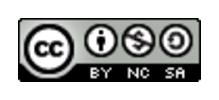
\includegraphics[width=0.15\hsize]{88x31.eps}
\end{flushright}

\section*{Acknowledgements}

Authors of this book would like to express special thanks to contributors to \XC{} implementation.
Among them, the following contributors work should be noted.

\subsection*{Mason Sharp}

Wrote initial version of backend global transaction management, planner and executor.

\subsection*{Pavan Deolasee}

Wrote initial GTM and GTM proxy.

\subsection*{Andrei Martsinchyk}

Wrote initial version of the pooler.

\subsection*{Abbas Butt}

Wrote online node addition/removal.
Also wrote many extensions including \texttt{RETURNING}, \texttt{LATERAL} and \texttt{CURSOR}.

\subsection*{Ashutosh Bapat}

Wrote most of the planner extension.

\subsection*{Amit Khandekar}

Wrote \texttt{TRIGGER}.

\subsection*{Ahsan Hadi}

Provided excellent project management in India and Pakistan side.

\subsection*{Michael Paquier}

Wrote various code including DDL propagation, DB2 and pgbench benchmark, among others.
He also contributed to clean up many bugs and codes.

\subsection*{Takayuki Sudo}

Built and maintained the buildfarm environment for \XC{} development, test and evaluation.

\subsection*{Nikhil Sontakke}

Contributed many GTM-related fixes.

\subsection*{Tetsuo Sakata}

Provided initial technical input to the project.

\subsection*{Hitoshi Hemmi}

Provided technical input and requirements to the project.

\subsection*{Masaki Hisada}

Provided technical input and requirements to the project.

%
% Change history referred by report.tex.
%

\chapter{Change History}

\paragraph*{\ReleaseDate}
Initial Document Release

% Repeat date and change contents.



%%%%%%%%%%%%%%%%%%%%%%%%%%%%%%%%%%%%%%%%%%%%%%%%%%%%%%%%%%%%%%%%%%%%%%%%%%%%%%%%%
%
% Main matter
%
%%%%%%%%%%%%%%%%%%%%%%%%%%%%%%%%%%%%%%%%%%%%%%%%%%%%%%%%%%%%%%%%%%%%%%%%%%%%%%%%%
\mainmatter

%%%%%%%%%%%%%%%%%%%%%%%%%%%%%%%%%%%%%%%%%%%%%%%%%%%%%%%%%%%%%%%%%%%%%%%%%%%%%%%%%
%
% PART 3: XC Technology Analysis
%
%%%%%%%%%%%%%%%%%%%%%%%%%%%%%%%%%%%%%%%%%%%%%%%%%%%%%%%%%%%%%%%%%%%%%%%%%%%%%%%%%
\newpage
\part{\label{part:analyzing}\XC{} Implementation}


%%%%%%%%% CHAPTER CHAPTER CHAPTER %%%%%%%%%%%%%%%%%%%%%%%%%%%%%%%%%%%%%%%%%%%%%%%%%%

% Postgres-XC Architecture: Koichi -- done.
\chapter{\label{chap:architecture}\XC{} Architecture}

%
% Architecture document comes here.
%

%
% Chapter/section, etc.  This section must exist in other file which includes archcontents.tex
% file.
%
\newcommand{\CHAP}[1]{\section{#1}}
\newcommand{\SEC}[1]{\subsection{#1}}
\newcommand{\SUBSEC}[1]{\subsubsection{#1}}
\newcommand{\ArchFig}{arch_doc/}

%%%%%%%%%%%%%%%%%%%%%%%%%%%%%%%%%%%%%%%%%%%%%%%%%%%%%%%%%%%%%%%%%%%%%%%%%%%%%%%%%%%%%%%%%%%%%%%%%%%
%
% Body of Postgres-XC architecture document
%
%%%%%%%%%%%%%%%%%%%%%%%%%%%%%%%%%%%%%%%%%%%%%%%%%%%%%%%%%%%%%%%%%%%%%%%%%%%%%%%%%%%%%%%%%%%%%%%%%%%
%
% \chapter or \section are macro here so that this is portable as separate document or as a part
% of other document.
%
%=================================================================================================



%%%%%%%%% CHAPTER CHAPTER CHAPTER %%%%%%%%%%%%%%%%%%%%%%%%%%%%%%%%%%%%%%%%%%%%%%%%%%

\CHAP{What is Postgres-XC?}

  Postgres-XC is an open source project to provide horizontal scalability including
  write-scalability, synchronous multi-master, and transparent PostgreSQL interface.
  It is a collection of tightly coupled database components which can be installed
  in more than one hardware or virtual machines.

  Write-scalability means Postgres-XC can be configured with as many database servers
  as you want and handle many more writes (updating SQL statements) than single
  database server can handle.
  Multi-master means you can have more than one data base servers which provides
  single database view.
  Synchronous means any database update from any database server is immediately visible
  to any other transactions running in different masters.
  Transparent means you don't have to worry about how your data is store
  in more than one database servers internally%
  \footnote{Of course, in order to get the most from Postgres-XC,
	you should consider when designing your schema where the table
	data will be physically stored.
  }.

  You can configure Postgres-XC to run on more than one physical or virtual servers.
  They store your data in a distributed way, that is,
  you can configure each table to be either partitioned or replicated%
  \footnote{
	To distinguish from \PG's partitioning, we call this ``\textbf{distributed}''.
	In distributed database textbooks, this is often referred to as a ``horizontal fragment''.
  }.
  When you issue queries, Postgres-XC determines where the target data
  is stored and issue appropriate SQL statements to servers which have the target
  data.
  This is shown in Figure~\ref{archfig:1}.

  % How XC looks like ... synchronous multi-master configuration
  \begin{figure}[htp]
    \begin{center}
      \includegraphics[width=\hsize]{\ArchFig ArchFig_01.eps}
      \caption{\label{archfig:1}\XC's synchronous multi-master configuration}
    \end{center}
  \end{figure}

  In typical web applications, you can use any number of web servers or application servers
  to handle your transactions.
  In general, you cannot do this for a database server because all the updates to the database
  have to be visible to all the transactions.
  Unlike other database cluster solution, Postgres-XC provides this capability.
  You can install as many database servers as you like. Each database server
  provides uniform data view to your applications.
  Any database update from any server is immediately visible
  to applications connecting the database from other servers.
  This feature is called ``synchronous multi master'' capability
  and this is the most significant feature of Postgres-XC,
  as illustrated in Figure~\ref{archfig:1}.

  Postgres-XC is based upon PostgreSQL database system and uses most of existing modules
  including interface to applications, parser, rewriter, planner and executor.
  In this way, \XC's application interface is compatible to existing PostgreSQL.
  (As described later, at present, \XC{} has some restrictions to SQL statements,
  mainly because of the distributed nature of the architecture.
  This will be improved in the future).



%%%%%%%%% CHAPTER CHAPTER CHAPTER %%%%%%%%%%%%%%%%%%%%%%%%%%%%%%%%%%%%%%%%%%%%%%%%%%

\CHAP{\XC's Goal}

  Ultimate goal of Postgres-XC is to provide synchronous multi-master \PG{} cluster
  with read/write scalability.
  That is, Postgres-XC should provide the following features:

  Postgres-XC should allow multiple servers to accept transactions and statements
  from applications,
  which is know as ``master'' server in general.
  In \XC, these components are called ``\textbf{coordinator}''.

  Any coordinator should provide consistent database view to applications.
  Any updates from any master must be visible in real time manner
  as if such updates are done in single PostgreSQL server.

  Tables should be able to be stored in the database in replicated or distributed way
  (known as fragment, shard or partition).
  Replication and distribution should be transparent to applications,
  that is, such replicated and distributed table are seen as single table
  and location or number of copies of each record/tuple is managed by
  \XC{} and is not visible to applications.

  \XC{} should provide compatible \PG{} API to applications.

  \XC{} should provide single and unified view of underlying \PG{} database servers
  so that SQL statements does not depend on how tables are stored in distributed way.

  So far, \XC's achievements are as follows:

  \begin{enumerate}

    \item Transaction management is almost complete.
		\PG{} provides complete ``Read Committed'' transaction isolation level
		which behaves exactly the same as single \PG{} server.
		Repeatable read, serializable and
		savepoint from the client should be added in the future.

    \item Major statement features are available.
		Some features, such as full cursor feature including \texttt{WHERE CURRENT OF},
		full constraint support in distributed table and savepoint are not supported.
		Background of some of them is the nature of table distribution and replication.
  
  \end{enumerate}


%%%%%%%%% CHAPTER CHAPTER CHAPTER %%%%%%%%%%%%%%%%%%%%%%%%%%%%%%%%%%%%%%%%%%%%%%%%%%

\CHAP{How To Scale Out Both Reads And Writes?}

  Simply put, parallelism is the key of the scalability.
  For parallelism, transaction control is the key technology.
  
  We'll compare \PG's transaction control with conventional replication clusters
  and show how \XC{} is safe to run update transactions in multiple nodes first,
  then shows major Postgres-XC components,
  and will finally show how to design the database to run transactions in parallel.

%========= SECTION SECTION ===================================================

\SEC{Parallelism In \XC}

  Parallelism is the key to achieve write scalability in \XC.
  
  Internally, \XC{} analyzes incoming SQL statement and chooses which server can handle it.
  It is done by a component called ``\textbf{coordinator}.''
  Actual statement processing is done by a component called ``\textbf{datanode}.''
  In typical transactional applications, each transaction reads/writes
  small number of tuples and lots of transactions has to be handled.
  In this situation, we can design the database so that one
  or a few datanodes are involved in handling each statement.
  
  In this way, as seen in Figure~\ref{archfig:2},
  statements are handled in parallel by Postgres-XC servers,
  which scales transaction throughput.
  As presented later in this document, with ten servers,
  the total throughput could be 6.4 compared with single server \PG.
  Please note that this is accomplished using conventional DBT-1 benchmark,
  which includes both read and write operation.
  Figure~\ref{archfig:2}  % Needs to refer to correct figure.
  shows that present \XC{} is suitable for transactional use case
  as described in \PG{} Wiki page.
  By improving supported SQL statements,
  we expect that \XC{} can be suitable for analytic use case.

  % Parallel statement handling in XC
  \begin{figure}[htp]
    \begin{center}
      \includegraphics[width=\hsize]{\ArchFig ArchFig_01_1.eps}
      \caption{\label{archfig:2}\XC{} can handle statements in parallel in multiple datanodes.}
    \end{center}
  \end{figure}

\SEC{Star Schema}

  There's a typical database schema structure called star schema%
  \footnote{
	  \url{http://www.ciobriefings.com/Publications/WhitePapers/DesigningtheStarSchemaDatabase/tabid/101/Default.aspx}
	  is a typical star schema description.
	  \url{https://www.youtube.com/watch?v=q77B-G8CA24} is a tutorial how to design start schema.
  }.
  It is found in many data warehouse and OLTP applications.
  Star schema consists of a few and big ``fact'' tables and many smaller ``dimension'' tables.
  For example, sales database may include ``sales fact'' as a fact table,
  as well as ``product dimension'' and ``store dimension'' table as dimension tables.
  Fact tables are big in size and updated frequently.
  On the other hand, dimension tables are small in size and more stable compared with fact tables.
  Figure~\ref{archfig:3} shows typical star schema%
  \footnote{The chart was taken from
	  \url{http://support.sas.com/documentation/cdl/en/spdsug/64018/HTML/default/viewer.htm#n0mlj75x9c4dtzn1ves84e1op3jt.htm}
  }.

  % Star schema example
  \begin{figure}[htp]
	  \begin{center}
		  \includegraphics[width=0.7\hsize]{\ArchFig star.eps}
		  \caption{\label{archfig:3}Typical star schema (See above for the source)}
	  \end{center}
  \end{figure}
 
  \XC{} architecture is build to leverage star schema characteristics.
  Usually, if there is more than one fact tables, they tend to share candidate keys.
  In \XC, it is desirable to shard fact tables using one of such common candidate key.
  In this way, we cay shard one (or few) big table into smaller pieces and store them
  in different server (datanode).
  The column used to determine what datanode each row goes is called a \textbf{distribution key}.
  
  Then updates by multiple transactions can be performed in more than one datanode in parallel.
  With more datanode, we can run more updates to fact tables in parallel.
  This is basically the background that Postgres-XC provides write scalability.
  Figure~\ref{archfig:4} illustrates this.
  
  % Updating smaller shards
  \begin{figure}[htp]
	  \begin{center}
		  \includegraphics[width=\hsize]{\ArchFig Arch_doc_fig_3_3.eps}
		  \caption{\label{archfig:4}Write scalability in \XC}
	  \end{center}
  \end{figure}
  
  As shown in Figure~\ref{archfig:5}, we replicate all the dimension tables to all the datanodes.
  Because most of the joins are done between a fact table and dimension tables,
  or among fact tables with distribution key involved,
  we can convert a big join to a union of smaller joins between each shard and replicated tables
  performed locally in each datanode in parallel.
  This is how \XC{} provides read scalability.

  % Join pushdown
  \begin{figure}[htp]
	  \begin{center}
		  \includegraphics[width=\hsize]{\ArchFig Arch_doc_fig_3_4.eps}
		  \caption{\label{archfig:5}Decomposing big statement into smaller shards}
	  \end{center}
  \end{figure}
  
  If a statement has additional predicates in \texttt{WHERE} clause which help to locate
  a datanode where the target rows are stored, then \XC{} can select only a few of
  datanode to perform such a query.
  This is found din many of OLTP workloads.
  
  Figure~\ref{archfig:5_1} illustrates this.
  
  % Join pushdown with WHERE clause
  \begin{figure}[htp]
	  \begin{center}
		  \includegraphics[width=\hsize]{\ArchFig Arch_doc_fig_3_5.eps}
		  \caption{\label{archfig:5_1}Statement can be optimized more
			  					      if \texttt{WHERE} clause determines the target}
	  \end{center}
  \end{figure}
  
  There could be exceptional case where an application needs a join between fact tables
  without distribution key involved.
  In this case, \XC{} pushes down as many operation as possible to each datanode
  and performs final join operation at the top level (coordinator).
  
  In other words, if an application cannot utilize this star schema, it is not suited to \XC.


%========= SECTION SECTION ===================================================

\SEC{Replicated table update: Primary node}

  Because of the delay in log-shipping replication,
  it is quite challenging to enforce consistent visibility
  and it is not practical to use log-shipping in replicated table update.
  
  To enforce data integrity in replicated tables, \XC{} uses a technique called
  ``\textbf{primary node}.''
  
  It is done in the following steps.
  
  % Replicated table update steps.
  \begin{enumerate}
	  \item Assign specific datanode as ``{\bf primary node}''.
	  \item Any write to replicated tables should go to the primary node first.
	  \item If there's any conflicting update, such update will be blocked at the primary node
	  		and conflicting update does not propagate to other datanode until current updating
			transaction is committed or aborted.
  \end{enumerate}
  
  Please note that this works with statement-based replication.
  This technique is similar to that used in pgpool-II's parallel mode.


%========= SECTION SECTION ===================================================

\SEC{\label{sec:ddlPropagation}DDL propagation}

  In \XC, most DDL should propagate to other coordinator and datanode as well.
  Exception is for node management DDL, such as \texttt{CREATE NODE} and \texttt{ALTER NODE}.  
  Node management DDL should run before each coordinator/datanode knows each other,
  automatic propagation was determined not practical.
  
  This restriction is not from the architecture but just an implementation issue.
  In the future, there could be an extension that the node management DDL propagates to
  other node automatically.


%========= SECTION SECTION ===================================================

\SEC{System catalog for shard and replica}

  In \XC, each table can be defined as ``distributed'' or ``replicated'' with \texttt{CREATE TABLE}
  \footnote{See \url{http://postgres-xc.sourceforge.net/docs/1_2_1/sql-createtable.html} for details}.
  and \texttt{ALTER TABLE}
  \footnote{See \url{http://postgres-xc.sourceforge.net/docs/1_2_1/sql-altertable.html} for details.}
  statements
  Distributed tables correspond to fact tables and replicated tables correspond to dimension tables
  in the star schema respectively.
  A distributed table is divided into shards using distribution key and stored in nodes as specified.
  You can specify how to locate each row, by hash, modulo or round-robin.
  A replicated table is copied to specified set of nodes and its content is maintained to be logically
  equivalent.
  
  \XC{} uses additional system catalog \file{pgxc_class}%
  \footnote{See \url{http://postgres-xc.sourceforge.net/docs/1_2_1/catalog-pgxc-class.html} for details.}
  to store sharding and replication information of each table.
  This can be an extension to \file{pg_class}.
  \XC{} chose to have this in a separate catalog so that changes in \PG{} and \XC{} can be maintained
  as separately as possible.


%========= SECTION SECTION ===================================================

\SEC{Limitations coming from sharding and replication}

  As described in section~\ref{archsec:3_5}, \XC{} uses SQL statement to instruct other nodes
  to do something.
  Because of this, \XC{} has following restrictions:
  
  % XC restriction on OID, CTID, global index and constraint due to XC architecture.
  \begin{enumerate}
	  \item Oid value may be different from node to node.
		    For example, you should not expect \file{pg_class} entry OID and other OID value
			in system catalogs are the same across the node.
			If you create a replicated table with OID, OID value will be different from node to node.
  
	  \item In replicated tables, CTIDs of given rows may be different from node to node.
  
	  \item Each shard of a distributed table has similar characteristics as inherited tables in \PG.
	  		Constraints across the shard is not simply supported.
			At present, \XC{} does not support unique index in a distributed table
			if the distribution column is not involved in index columns.
			For the same reason, referential integrity between distributed tables
			are not supported unless it is guaranteed to be maintained locally.
  \end{enumerate}
  
  Restrictions and remarks for specific SQL statement will be given in a separate material.


%========= SECTION SECTION ===================================================

\SEC{\label{archsec:3_5}\XC's Global Transaction Management}

  This section describes how transaction update and visibility are enforced in \XC.
  You may need to be familiar with internal of PostgreSQL transaction management
  infrastructure such as \texttt{XID}, snapshot, \texttt{xmin} and \texttt{xmax}.
  This information is found in ``MVCC revealed'' available at
  \url{http://momjian.us/main/writings/pgsql/mvcc.pdf}
  
  In replication clusters, you can run read transactions in parallel in multiple standby,
  or slave servers.
  Replication servers provide read scalability.
  However, you cannot issue write transactions to standby servers
  because they don't have means to propagate changes in slaves
  They cannot maintain consistent view of database to applications for write operations,
  unless you issue write transactions to single master server.
  
  \XC{} is different.
  
  \XC{} is equipped with global transaction management capability which provides
  cluster-wide transaction ordering and cluster-wide transaction status to transactions
  running on the coordinator (master) and the node which really stores the target data
  and runs statements, called datanode.
  This maintains ACID property for distributed transaction and provide atomic visibility%
  \footnote{
	  ``Scalable Atomic Visibility with RAMP Transactions,''
	  SIGMOD'14, June 22 -- 27, 2014, Snowbird, UT, USA,
	  \url{http://www.bailis.org/papers/ramp-sigmod2014.pdf}
  }
  to transactions reading more than one node.
  
%========= SECTION SECTION ===================================================

\SEC{Statement based replication and sharding}

  At present, Postgres-XC sends SQL statements to other nodes to read and write tables.
  There are many discussions if it is a right choice,
  or if we should use internal plan tree to transfer to other node.
  
  An internal analysis of dynamic behavior of PostgreSQL shows that
  around 30\% of CPU resource is consumed to parse and plan a statement for typical OLTP workloads.
  Saving this resource looks nice.
  On the other hand, serialized plan tree can be very big, which suffers network workload.
  We also need to maintain all the internal information such as Oids and ctids
  throughout \XC{} cluster, which are not simple.
  They are the main reason why Postgres-XC chose to send statement from node to node.
  
  Because of this and parallelism of transactions and statements,
  \XC{} does not maintain Oids and ctids of each object and row.


%%%%%%%%% CHAPTER CHAPTER CHAPTER %%%%%%%%%%%%%%%%%%%%%%%%%%%%%%%%%%%%%%%%%%%%%%%%%%

\CHAP{\XC{} Key Components}

  In this section, major components of \XC{} will be described.
  
  \XC{} is composed of three major components, called \textbf{GTM} (Global Transaction Manager),
  \textbf{Coordinator} and \textbf{Datanode} as shown in Figure~\ref{archfig:6}.
  Their features are given in the following sections.
  
  % Postgres-XC components
  \begin{figure}[htp]
	  \begin{center}
		  \includegraphics[width=\hsize]{\ArchFig ArchFig_03_6.eps}
		  \caption{\label{archfig:6}\XC{} Key Components}
	  \end{center}
  \end{figure}
  
  Figure~\ref{archfig:7} outlines how each key component interacts.
  
  % Interaction among Postgres-XC components
  \begin{figure}[htp]
	  \begin{center}
		  \includegraphics[width=\hsize]{\ArchFig ArchFig_03_7.eps}
		  \caption{\label{archfig:7}Interaction between \XC{} key components}
	  \end{center}
  \end{figure}


%========= SECTION SECTION ===================================================

\SEC{\label{arch:4_1}GTM (Global Transaction Manager)}

  GTM is a key component of \XC{} to provide consistent transaction management
  and tuple visibility control.
  First, we will give how \PG{} manages transactions and database update.

%------- Subsec Subsec -----------------------------------------------------

\SUBSEC{How PostgreSQL Manages Transactions}

  In \PG, each transaction is given unique ID called transaction ID (or XID).
  XID is given in ascending order to determine which transaction is older/newer%
  \footnote{
	  More precisely, XID is unsigned 32bit integer.
	  When XID reaches the max value,
	  it wraps around to the lowest value (3, as to the latest definition).
	  \PG{} has a means to handle this, as well as \XC.
	  For simplicity, it will not be described in this document
  }.
  Please let us describe a little in detail how it is done%
  \footnote{
	  Please note that this description is somewhat simplified for explanation.
	  You will find the precise rule in \file{tqual.c} file in \PG's source code.
  }.
  
  When a transaction tries to read a tuple, each tuple has a set of XIDs
  to indicate transactions which created and deleted the tuple.
  So if the target tuple is created by an active transaction,
  it is not committed or aborted and reading transaction should ignore such tuple.
  In such way (in practice, this is done by \file{tqual.c} module in \PG{} core),
  if we give each transaction a unique transaction Id throughout the system
  and maintain snapshot what transaction is active,
  not only in a single server but transaction in all the servers,
  we can maintain global consistent visibility of each tuple
  even when a server accepts new statement from other transactions running only on other servers.
  
  These information is stored in ``\texttt{xmin}'' and ``\texttt{xmax}'' fields of each row of table.
  When we \texttt{INSERT} rows, XID of inserting transaction is recorded at xmin field.
  When we update rows of tables (with \texttt{UPDATE} or \texttt{DELETE} statement),
  \PG{} does not simply overwrite the old rows.
  Instead, \PG{} ``marks'' old rows as ``deleted'' by writing updating transaction's XID
  to \texttt{xmax} field.
  In the case of \texttt{UPDATE} (just like \texttt{INSERT}),
  new rows are created whose \texttt{xmin} field is ``marked'' with XIDs of the creating transaction.
  
  These ``\texttt{xmin}'' and ``\texttt{xmax}'' are used to determine which row is visible
  to a transaction.
  To do this, \PG{} needs a data to indicate what transactions are running at specific time.
  This is called ``\textbf{snapshot}.''
  If a transaction is in a snapshot, it is regarded as \textbf{running} even though it has finished.

  You should understand that this specific time is not just \textbf{now}.
  If isolation level of a transaction is \texttt{read committed}, the transaction needs consistent
  visibility for some period of time, at least while an SQL statement is being executed.
  It is not preferable if SQL statements reads sone rows which are committed during this execution.
  Therefore, in the case of \texttt{read committed} isolation level, database should obtain a
  snapshot before the execution of a statement and continue to use it throughout the execution.

  % The above does not describe xmax precisely.   Each snapshot should include xmax, which is
  % the maximum xid every stated.  At visibility test, if a transaction is not found in the
  % snapshot and its xid is larger than xmax, the transaction started after the snapshot was
  % obtained so the transaction is not visible.
  % If xid is less than xmax, then the transaction should have started when the snapshot was
  % obtained so the visibility depends upon clog.
  %
  % Unfortunately, it has not been implemented at current GTM precisely.
  % Also, we need an improvement of recent xmin calculation.

  In the case of \texttt{repeatable read} and \texttt{serializable}, the transaction need
  consistent visibility throughout the transaction execution.
  In this case, the transaction should obtain the snapshot before statement execution and should
  continue to use it throughout the transaction execution, not single statement execution.
  
  If a transaction which created the row is not running,
  visibility of each row depends upon the fact if the creating transaction was
  committed or aborted.
  Suppose a row of a table which was created by some transaction and is not deleted yet.
  If the creating transaction is running, such row is visible to the transaction
  which created the row, but not visible to other transactions.
  If the creating transaction is not running and was committed the row is visible.
  If the transaction was aborted, this row is not visible.
  
  Therefore, \PG{} needs two kinds of information to determine
  ``{\it which transaction is running}'' and
  ``{\it if an old transaction was committed or aborted}.''
  
  The former information can be obtained as ``snapshot.''
  \PG{}  maintains the latter information as ``CLOG.''
  
  \PG{} uses all these information to determine which row is visible to a given transaction.


%------- Subsec Subsec -----------------------------------------------------

\SUBSEC{Making Transaction Management Global}

  In \XC, GTM provides the following feature for transaction management:
  
  % TXN management feature provided by GTM.
  \begin{enumerate}
  
	  \item Assigning XID globally to transactions (GXID, Global Transaction ID).
	  		With GXID, global transactions can be identified globally.
			If a transaction writes to more than one node, we can track such writes.`
  
	  \item Providing snapshot. GTM collects all the transaction's status
	  		(running, committed, aborted etc.~ to provide snapshot globally (global snapshot).
  			Please note that global snapshot includes GXID given to other servers as
			shown in Figure~\ref{archfig:7}.
  			This is needed because some older transaction may visit new server after a while.
  			In this case, if GXID of such a transaction is not included in the snapshot,
  			this transaction may be regarded as ``{\it old enough}'' and uncommitted
			rows may be read.
  			If GXID of such transaction is included in the snapshot from the beginning,
			such inconsistency does not occur.
  
  \end{enumerate}
  
  The reason why we need a global snapshot is as follows:
  
  2PC protocol enforces update of each distributed transaction.
  However, it does not enforce to maintain the consistent visibility of a distributed transaction
  updates to others.
  Depending upon the timing of commit at each node, the update may or may not be visible to
  the same transaction which reads these nodes.
  To maintain the consistent visibility, we need a global snapshot
  which includes all the running transaction information (GXID, global transaction id, in this case)
  in \XC{} cluster and use it in the same context of the read operation as found in \PG.
  
  To do this, \XC{} introduced a dedicated component called GTM (Global Transaction Manager).
  GTM runs as a separate component and provide unique and ordered transaction id to each transaction
  running on \XC{} servers%
  \footnote{
	  You can configure GTM in the same server as other components such as coordinator and datanode
  }.
  We call this GXID (Global Transaction Id) because this is globally unique ID,
  
  GTM receives GXID request from transactions and provide GXID.
  It also keep track of all the transactions when it started and finished to generate snapshot
  used to control each tuple visibility.
  Because snapshot here is also global property, it is called Global Snapshot.
  
  As long as each transaction runs with GXID and Global Snapshot,
  it can maintain consistent visibility throughout the system and it is safe to run transactions
  in parallel in any servers.
  On the other hand, a transaction, composed of multiple statements, can be executed
  using multiple servers maintaining both update and visibility consistently.
  Outline of this mechanism is illustrated in Figure~\ref{archfig:8}.
  Please note how transactions included in each snapshot changes according to global transaction.
  
  % Global Transaction Management Outline
  \begin{figure}[htp]
	  \begin{center}
		  \includegraphics[width=0.8\hsize]{\ArchFig ArchFig_04_2.eps}
		  \caption{\label{archfig:8}Outline of \XC's Global Transaction Management}
	  \end{center}
  \end{figure}
  
  GTM provides Global Transaction Id to each transaction and keeps track of the status of
  all the transactions, whether it is running, committed or aborted, to calculate global
  snapshot to maintain tuple visibility.
  
  Please note that each transaction reports when it starts and ends, as well as when it
  issues \texttt{PREPARE TRANSACTION} command in two-phase commit protocol.
  
  Please also note that global snapshot provided by GTM includes other transactions running
  on other components.
  
  Each transaction requests snapshot according to the transaction isolation level as done
  in PostgreSQL.
  If the transaction isolation level is ``\texttt{read committed}'', then transaction will request
  a snapshot for each statement%
  If it is ``\texttt{repeatable read},''
  \footnote{PostgreSQL has another isolation level ``\texttt{serializable}'', based upon SSI.
	 		Although it seems that global snapshot works well with SSI, this may need further
	  		discussion and study.
  }
  transaction will request a snapshot at the beginning of transaction and reuse it
  throughout the transaction.
  
  GTM also provides global value such as sequence.
  Other global properties such as timestamps and notification will be an extension
  in the following releases%
  \footnote{
	  GTM provides timestamp and is used to some extent at present.
  }.


%========= SECTION SECTION ===================================================

\SEC{Coordinator}

  Coordinator is an interface to applications.
  It acts like conventional PostgreSQL backend process.
  However, because tables may be replicated or distributed, coordinator does not store
  any actual data.
  Actual data is stored by Datanode as described below.
  Coordinator receives SQL statements, get Global Transaction Id and Global Snapshot as needed,
  determine which datanode is involved and ask them to execute (whole or a part of) the statement.
  When issuing statement to datanodes,
  coordinator propagates GXID and Global Snapshot to run the statement at datanodes in the same
  transaction context.


%========= SECTION SECTION ===================================================

\SEC{Datanode}

  Datanode actually stores user data.
  Tables may be distributed among datanodes, or replicated to all the datanodes.
  Datanode does not handle global view of the whole database and just takes
  care of local data.
  Coordinator builds the statement to run in the datanode locally.
  Incoming statement is examined by the coordinator as described next, and rebuilt
  to execute at each datanode involved.
  It is then transferred to each datanodes involved together with GXID and Global
  Snapshot as needed.
  Datanode may receive request from various coordinators.
  However, because each the transaction is identified uniquely and associated with
  consistent (global) snapshot, datanode doesn't have to worry what coordinator
  each transaction or statement came from.
  
  Overall diagram of transaction control and query processing is shown in Figure~\ref{archfig:9}.
  
  % Interaction among components.
  \begin{figure}[htp]
	  \begin{center}
		  \includegraphics[width=0.8\hsize]{\ArchFig ArchFig_04_3.eps}
		  \caption{\label{archfig:9}Interaction among \XC{} components}
	  \end{center}
  \end{figure}
  

%========= SECTION SECTION ===================================================

\SEC{Interaction Between Key Components}

  As explained in the previous section, \XC{} has three major components to provide
  global consistency of both multi-node reads and writes and to determine which datanode each
  statement should go and to handle the statement.
  
  Sequence of global transaction control and interaction among \XC{} components are
  given in Figure~\ref{archfig:10}.
  
  % Sequence of transaction control
  \begin{figure}[htp]
	  \begin{center}
		  \includegraphics[width=\hsize]{\ArchFig ArchFig_03.eps}
		  \caption{\label{archfig:10}Sequence of Global Transaction Control}
	  \end{center}
  \end{figure}
  
  As shown in the figure, when a coordinator begins a new transaction, it requests GTM
  for new transaction ID (GXID, global transaction id).
  GTM keeps track of such requirement to calculate global snapshot.
  
  If the transaction isolation mode is \texttt{REPEATED READ}, snapshot will be obtained and
  used throughout the transaction.
  When the coordinator accepts a statement from an application and the isolation mode is
  \texttt{READ COMMITTED}, snapshot will be obtained from the GTM.
  Then the statement is analyzed, determined what datanode to go, and converted for
  each datanode if necessary.
  
  Please note that statements will be passed to appropriate datanodes with GXID
  and global snapshot to maintain global transaction Identity and visibility of
  each rows of tables.
  Each result is be collected and calculated into the response to the application.
  
  At the end of the transaction, if multiple datanodes are involved in the update in
  the transaction, the coordinator issues \texttt{PREPARE TRANSACTION} for 2PC, then issue
  \texttt{COMMIT}.
  These steps will be reported to GTM as well to keeps track of each transaction
  status for the calculation of subsequent global snapshots.
  
  Please see the section~\ref{arch:4_1} for details of this background.



%%%%%%%%% CHAPTER CHAPTER CHAPTER %%%%%%%%%%%%%%%%%%%%%%%%%%%%%%%%%%%%%%%%%%%%%%%%%%

\CHAP{Isn't GTM A Performance Bottleneck}

  Because GTM can be regarded as ``serializing'' all the transaction processing,
  it could be a performance bottleneck.
  
  In fact, GTM can limit the whole scalability.
  GTM should not be used in very slow network environment such as wide area network.
  GTM architecture is intended to be used with Gigabit local network.
  For the network workload, please see section~\ref{Arch_Net_Workload}.
  Latency to send each packet may be a problem.
  We encourage to install \XC{} with local Gigabit network with minimum latency
  that is, use as fewer switches involved in the connection among GTM,
  coordinator and datanodes.
  Typical configuration is shown in Figure~\ref{archfig:11}.
  
  This chapter describes general performance issue of GTM in \XC{} along with
  GTM internal structure alternatives.
  
  % GTM configuration without GTM Proxy
  \begin{figure}[htp]
	  \begin{center}
		  \includegraphics[width=\hsize]{\ArchFig ArchFig_04.eps}
		  \caption{\label{archfig:11}GTM Configuration without GTM Proxy}
	  \end{center}
  \end{figure}
  

%========= SECTION SECTION ===================================================

\SEC{\label{archsec:5_1}GTM Implementation without proxy}
  
  Sequence in Figure~\ref{archfig:10}, can be implemented as shown in
  Figure~\ref{archfig:11}.
  Coordinator backend corresponds to \PG's backend process which handles
  a database connection from an application and handles each transaction.
  
  The outline of the structure and algorithm are as follows:
  
  % Outline of the structure and algorithm of GTM w/o proxy.
  \begin{enumerate}
	  \item Coordinator backend is provided with GTM client library to obtain GXID and
	  		snapshot and to report the transaction status.
	  \item GTM opens a port to accept connection from each coordinator backend.
	  		When GTM accepts a connection, it creates a thread (GTM Thread) to handle
			request to GTM from the connected coordinator backend.
	  \item GTM Thread receives each request, record it and returns GXID, snapshot and
	  		other response to the coordinator backend.
	  \item The above sequence is repeated until the coordinator backend requests
	  		disconnect.
  \end{enumerate}
  
  Each of the above interaction is done separately.
  For example, if the number of coordinator is ten and each coordinator has
  one hundred connection from applications, which is quite reasonable in
  single \PG{} in transactional applications, GTM has to have one thousand of
  GTM Threads.
  If each backend issues 25 transaction in a second and each transaction includes
  five statements and each coordinator runs one hundred backends,
  then the total number of the interaction between GTM and
  ten coordinators to provide global snapshot can be estimated as:
  $10\times 100\times 25\times 5 = 125,000$.
  Because we have one hundred backends in each coordinator, the length of snapshot
  (GXID is 32bit integer, as defined in \PG) will be $4 \times 100 \times 10 = 4,000$Bytes.
  Therefore, GTM has to send about 600Megabytes of data in a second to support this scale.
  It is quite larger than Gigabit network can support%
  \footnote{In later section, you will see this estimation is too large. However, this can
	  be a bottleneck anyway.
  }.
  In fact, the order of the amount of data sent from GTM is $O(N^2)$ where $N$ is
  the number of coordinators.
  
  Not only the amount of data is the issue.
  The number of interaction is an issue.
  Very simple test will show that Gigabit network provides up to $100,000$ interactions for
  each server.
  
  Network workload measurement in later section shows the amount of data is
  not that large, but it is obvious that we need some means to reduce both
  interaction and amount of data.
  
  The next section will explain how to reduce both the number of interaction and
  amount of data in GTM.


%========= SECTION SECTION ===================================================

\SEC{\label{arch:5_2}GTM Proxy Implementation}

  You may have been noticed that each transaction is issuing request to GTM so
  frequently and we can collect them into single block of requests in each
  coordinator to reduce the amount of interaction.
  
  This is the idea of GTM Proxy Implementation as shown in Figure~\ref{archfig:12}.
  
  % GTM configuration with GTM Proxy
  \begin{figure}[htp]
	  \begin{center}
		  \includegraphics[width=0.95\hsize]{\ArchFig ArchFig_05.eps}
		  \caption{\label{archfig:12}GTM Configuration with GTM Proxy}
	  \end{center}
  \end{figure}
  
  In this configuration, each coordinator backend does not connect to GTM directly.
  Instead, we have GTM Proxy between GTM and coordinator backend to group multiple
  requests and responses.
  GTM Proxy, like GTM explained in Section~\ref{archsec:5_1}, accepts connection from
  the coordinator backend.
  However, it does not create new thread.
  The following paragraphs explains how GTM Proxy is initialized and how it handles
  requests from coordinator backends.
  
  GTM Proxy, as well as GTM, is initialized as follows:
  
  % Initialization of GTM proxy and GTM
  \begin{enumerate}
	  \item GTM starts up just as described in section~\ref{archsec:5_1}.
	  		Now GTM can accept connections from GTM Proxies.
	  \item GTM Proxy starts up.
  			GTM Proxy creates GTM Proxy Threads.
  			Each GTM Proxy Threads connect to the GTM in advance.
  			The number of GTM Proxy Threads can be specified at the startup.
  			Typical number of threads is one or two so it can save the number of
			connections between GTM and Coordinators.
	  \item GTM Main Thread waits for the request connection from each backend.
  \end{enumerate}
  
  When each coordinator backend requests for connection, Proxy Main Thread assigns
  a GTM Proxy Thread to handle request.
  Therefore, one GTM Proxy Thread takes care of multiple coordinator backends.
  If a coordinator has one hundred coordinator backends and one GTM Proxy Thread,
  this thread takes care of one hundred coordinator backends.
  
  Then GTM Proxy Thread scans all the requests from coordinator backend.
  If coordinator is busier, it is expected to capture more requests in
  a single scan.
  Therefore, the proxy can group many requests into single block of requests,
  to reduce the number of interaction between GTM and the coordinator.
  
  Furthermore, in a single scan, we may have multiple request for snapshots.
  Because these requests can be regarded as received at the same time, we can
  represent multiple snapshots with single one.
  This will reduce the amount of data which GTM provides.
  
  Test result will be presented later but it is observed that the GTM Proxy is applicable to
  twenty coordinators at least in short transactional application such as DBT-1.
  
  It is not simple to estimate the order of interaction and amount of data in
  GTM Proxy structure.
  When the workload to \XC{} is quite light, the interaction will be as same as the case in
  Section~\ref{archsec:5_1}.
  On the other hand, when the workload is heavier, the amount of data is expected to be
  smaller than $O(N^2)$ and the number of interaction will be smaller than $O(N)$.


%%%%%%%%% CHAPTER CHAPTER CHAPTER %%%%%%%%%%%%%%%%%%%%%%%%%%%%%%%%%%%%%%%%%%%%%%%%%%

\CHAP{Performance And Stability}

%========= SECTION SECTION ===================================================

\SEC{\label{arch:dbt1}DBT-1-Based Benchmark}

  DBT-1 benchmark is used as a basis of performance and stability evaluation.
  We chose DBT-1 benchmark for the test because
  
  % Why we chose DBT-1 as PGXC benchmark?
  \begin{itemize}
	  \item It is a typical OLTP workload benchmark available in public for transactional use case.
	  \item Tables cannot be partitioned simply with single common distribution key.
	  		We need more than one distribution key.
  \end{itemize}
  
  The following describes how DBT-1 was modified to best tune to \XC.
  To localize each statement target, we modified DBT-1 tables as follows%
  \footnote{
  	Tables are designed so that it cannot simply be partitioned.
	We need more than one partitioning key.
  }.
  
  % Outline of DBT-1 modification
  \begin{enumerate}
	  \item Customer-ID is added to \file{ADDRESS} table because it is practically
	  		obvious that personal information belongs to each customer and
			it is common practice not to share such information among different customers.
	  \item Stock table is divided into two tables, item and stock, as in the latest
	  		TPC-W specification.
  \end{enumerate}
  
  Also, we changed connection from ODBC to libpq%
  \footnote{
  	This is because early \XC{} implementation did not support ODBC
  }.
  
  Table configuration of DBT-1 is illustrated in Figure~\ref{archfig:15} with
  modification for Postgres-XC.
  Tables with blue frame are distributed using customer ID, green with shopping
  cart ID and red with item ID.
  Tables with black frame are replicated over all the datanodes.
  
  % DBT-1 table structure
  \begin{figure}[htp]
	  \begin{center}
		  \includegraphics[width=\hsize]{\ArchFig ArchFig_14_1.eps}
		  \caption{\label{archfig:15}DBT-1-Based Table Structure Used in the Benchmark}
	  \end{center}
  \end{figure}
  
  Please note the distribution of \file{SHOPPPING_CART} cart and \file{SHOPPING_CART_LINE} tables.
  It is more favorable if shopping cart and shopping card ID can be distributed using
  customer ID.
  However, DBT-1 uses these table even while a customer is not assigned to the shopping cart.
  This is the reason they are distributed using shopping cart ID.
  
  We also found that current DBT-1 is not suitable for long-period test.
  DBT-1 does not maintain order and order line tables.
  From time to time, number of outstanding order increases while some of the
  transaction displays all such orders.
  Number of displayed order could be thousands and could reduce the throughput as we measure it
  for a long period as one week.
  
  To improve this, we modified the code to limit the number of displayed order.
  (the modification is available as a part of \XC{} release material).
  
  Test environment is shown in Figure~\ref{archfig:16}.
  We have one GTM, and up to ten database servers.
  Each server is configured with one coordinator and one datanode.
  Although we can install coordinator and datanode in separate servers, we used this
  configuration because it is simpler to balance the workload of coordinator and datanode.
  
  % DBT-1 Test Environment
  \begin{figure}[htp]
	  \begin{center}
		  \includegraphics[width=\hsize]{\ArchFig ArchFig_14_2.eps}
		  \caption{\label{archfig:16}\XC{} Test Environment}
	  \end{center}
  \end{figure}
  
  Additional four servers were used to generate DBT-1 workloads.
  
  Each servers are equipped with two NICs (1Gbps each).
  GTM and some of coordinator are equipped with Infiniband connection to be used when
  Gigabit network is not sufficient.
  Preliminary experiment showed that Infiniband is not required for this case.
  Infiniband is suitable for the workload to use giant packet.
  DBT-1 workload in \XC{} does not use giant packet.


%%%%%%%%% CHAPTER CHAPTER CHAPTER %%%%%%%%%%%%%%%%%%%%%%%%%%%%%%%%%%%%%%%%%%%%%%%%%%

\CHAP{Test Result}

  This section describes the benchmark test using DBT-1 based benchmark program and
  environment described in previous sections.
  
  We ran the benchmark program in the following configuration.
  
  % Configurations for DBT-1 benchmark
  \begin{enumerate}
	  \item Vanilla PostgreSQL for reference.
	  \item \XC{} with one server.
	  \item \XC{} with two servers.
	  \item \XC{} with three servers.
	  \item \XC{} with five servers.
	  \item \XC{} with ten servers.
  \end{enumerate}
  
  One coordinator and datanode were installed in each server.
  GTM was installed in a separate server.
  GTM-Proxy was optional to measure its effort to network workload.
  We ran the test with two kinds of workload as follows:
  
  % Benchmark workload
  \begin{enumerate}
	  \item Full load. Measured throughput and resource consumption with full workload, which is
	  		the maximum throughput available.
	  \item 90\% load. Arranged workload to get 90\% throughput of the full load.
  \end{enumerate}
  
  The following sections will explain the throughput, scale factor, resource consumption and
  network workload of the benchmark.


%========= SECTION SECTION ===================================================

\SEC{Throughput and Scalability}

  This subsection describes the measurement result of throughput and scale factor.
  
  Table~\ref{archtab:1} shows the result of full load throughput for various configurations.
  Figure~\ref{archfig:18} is the chart of Postgres-XC scale factor vs.~ number of servers,
  based on the result in Table~\ref{archtab:1}.
  
  % Full workload benchmark test result (throughput)
  \begin{table}[htp]
	  \begin{center}
		  \caption{\label{archtab:1} Summary of measurement (Full load)}
		  \begin{tabular}{|c|c|c|c|} \hline
			  Database & Num.of Servers&Throughput (TPS)&Scale Factor\\\hline
			  \PG&1&2,500&$1.0$\\\hline
			  \XC{}&1&1,900&$0.72$\\\hline
			  \XC{}&2&3,630&$1.45$\\\hline
			  \XC{}&3&5,568&$2.3$\\\hline
			  \XC{}&5&8,500&$3.4$\\\hline
			  \XC{}&10&16,000&$6.4$\\\hline
		  \end{tabular}
	  \end{center}
  \end{table}
  
  
  % DBT-1 Test Result
  \begin{figure}[htp]
	  \begin{center}
		  \includegraphics[width=0.8\hsize]{\ArchFig ArchFig_14_3.eps}
		  \caption{\label{archfig:18}\XC{} Full Load Throughput}
	  \end{center}
  \end{figure}
  
  From these table and figure, scale factor is quite reasonable, considering that each statements
  parsed and analyzed twice, by coordinator and datanode.
  
  We also ran \XC{} with five coordinators/datanodes for a week with 90\% workload of
  the full load with five coordinator/datanodes.
  In this period, GTM, coordinators and datanodes handled GXID wraparound and vacuum freeze successfully.%
  \footnote{
  	Because GXID, as well as TransactionID in PostgreSQL, is defined as 32bit unsigned integer,
	it reaches the maximum value some time (in this case, on 6th or 7th day) and GXID value has
	to return to the initial valid value.
  	Until then, all the tuples marked with the first half value of GXID has to be frozen to
	special XID value defined as \texttt{FrozenTransactionId}.
  }
  \footnote{
  	Please note that this measurement is a bit different from the official scaling chart used today.
  	The original document is based upon older measurement.
  	For more precise analysis, we need to rerun the benchmark again with the current hardware.
  }
  
  Figure~\ref{archfig:17} shows the throughput chart. At average, the throughput is quite stable,
  except that spikes are observed periodically and spike grows with time.
  
  % Postgres-XC 90% Load Throughput in One Week Test
  \begin{figure}[htp]
	  \begin{center}
		  \includegraphics[width=0.8\hsize]{\ArchFig ArchFig_14_4.eps}
		  \caption{\label{archfig:17}\XC{} 90\% Load Throughput in One Week Test}
	  \end{center}
  \end{figure}



%========= SECTION SECTION ===================================================

\SEC{CPU Consumption}

  We've measured CPU consumption in the benchmark test above to see if
  \XC{} reasonably uses hardware resource.
  Table~\ref{tab:ArchCPU} shows CPU usage ($100\% - \mbox{idle}$) for
  various configuration and nodes with full workload.
  
  % --- CPU Usage Table -----------------------------
  \begin{table}[htp]
	  \begin{center}
		  \caption{\label{tab:ArchCPU} \XC{} CPU Usage}
		  \begin{tabular}{|c|c|c|c|}
			  \hline
			  Configuration&GTM&CO/DN$^{*}$(Av.)&Loader(Av.)\\\hline
			  \PG$^{**}$&N/A&99.2\%&5.6\%\\\hline
			  \XC(1,2)$^{***}$&1.9\%&91.5\%&5.1\%\\\hline
			  \XC(2,2)$^{***}$&3.9\&&95.6\%&11.7\%\\\hline
			  \XC(3,2)$^{***}$&6.5\%&96.4\%&19.3\%\\\hline
			  \XC(5,2)$^{***}$&14.3\%&96.4\%&38.0\%\\\hline
			  \XC(10,4)$^{***}$&42.2\%&95.7\%&34.4\%\\\hline
		  \end{tabular}

		  {\footnotesize
			{}$^{*}$~Coordinator/Datanode\\
			{}$^{**}$~2 loaders were used.\\
			{}$^{***}$~Indicates number of Coordinator/Datanode and loader respectively.}
  
	  \end{center}
  \end{table}


%========= SECTION SECTION ===================================================

\SEC{\label{Arch_Net_Workload}Network Workload}

  We measured the network workload as well.
  
  Figure~\ref{Archfig:13_2} summarizes the data transfer rate among each component.
  
  This is also summarized in Table~\ref{Archtab:2}.
  
  % Network transfer rate
  \begin{figure}[htp]
	  \begin{center}
		  \includegraphics[width=\hsize]{\ArchFig ArchFig_13.eps}
		  \caption{\label{Archfig:13_2}Network Data Transfer Rate of Each Server}
	  \end{center}
  \end{figure}
  
  % Network Workload
  \begin{table}[htp]
	  \begin{center}
		  \caption{\label{Archtab:2} \XC{} Network Workload}
		  \begin{tabular}{|p{4.5cm}|c|c|c|c|} \hline
			  Server&Read(simple)&Read(proxy)&Write(simple)&Write(proxy)\\\hline
			  GTM $\Leftrightarrow$ Coordinator&3.3MB/s&1.7MB/s&59.3MB/s&28.6MB/s\\\hline
			  Loader $\Leftrightarrow$ Coordinator&14.0MB/s&16.8MB/s&2.5MB/s&2.6MB/s\\\hline
			  Coordinator/Datanode $\Leftrightarrow$ Loader/GTM&7.0MB/s&3.8MB/s&6.8MB/s&8.6MB/s\\\hline
			  Coordinator/Datanode $\Leftrightarrow$ Coordinator/Datanode&4.8MB/s&5.1MB/s&4.8MB/s&4.8MB/s\\\hline
		  \end{tabular}
	  \end{center}
  \end{table}
  
  This measurement indicates the following:
  
  \begin{enumerate}
	  \item GTM Proxy drastically reduces the amount of data transfer between GTM and coordinator.
	  		Considering the network transfer rate about 100GB/s (Gigabit network), GTM can
			take care of at least twenty coordinators at full load.
	  \item Other server's network workload is very light.   Conventional Gigabit network is
	  		sufficient.
  \end{enumerate}


%========= SECTION SECTION ===================================================

\SEC{Connection Handling}

  We want to avoid involving datanodes in a transaction
  that do not have target data.
  That is, we do not simply obtain a connection to every datanode for every client
  session connected to a coordinator.
  The connections are managed via a connection pooler process.
  
  For example, assume we have two tables each distributed across 10 nodes via a hash on one
  of their respective columns.
  If we have a two statement transaction (each an \texttt{UPDATE}) where the \texttt{WHERE}
  clause of each \texttt{UPDATE} contains the hash column being compared to a literal,
  for each of those statements we can determine the single node to execute on.
  When each of those statements is executed, we only send it down to the
  datanode involved. 
  
  Assume in our example, only 2 datanodes were involved, one for the
  first \texttt{UPDATE} statement, and one for the second one.
  This frees up more connections that can remain available in the pool. In addition,
  at commit time, we commit on only those nodes involved. 
  
  Again using this example, we implicitly commit the transaction in a two-phase commit
  transaction since more than one datanode is involved. 
  Note that if both of the \texttt{UPDATE}s went to the same data
  node, at commit time we detect this and do not bother using two phase
  commit, using a simple commit instead.


%========= SECTION SECTION ===================================================

\SEC{High-Availability Consideration}

  In High-Availability (HA, afterwords) solution, we need to integrate automatic
  failover system not only for \XC{} components but also for other system components
  such as server hardware, storage system and network.
  
  Because this integration deeply depends upon specific cases, it is determined that
  such HA integration/solution is outside \XC{} scope, as in the case of vanilla \PG.
  
  Instead, \XC's component provides each slave which is available in integrating
  into system-wide HA solution.
  
  So far, gtm proxy does not have any permanent data in it and it does not need
  specific consideration for HA.
  
  Coordinator and datanode uses vanilla \PG's log-shipping replication.  To minimize
  transaction loss chance, it is highly recommended to connect with slave using
  synchronous replication.
  
  GTM needs separate slave feature.
  In this case, GTM can copy all its status changes such as GXID and sequence values
  to the slave.
  



% Postgres-XC Source code tree structure: Koichi -- done.
\chapter{\label{chap:sourceTree}\XC{} source code tree structure}

  The rest of this part describes major implementation details of \XC.
  It is based upon the source code of \file{REL1_2_STABLE} branch of \XC{} git repository.
  
  In referring source file, directofy path may not be given or only a part of it may be
  given if there's no ambiguity.

%
% Chapter "Postgres-XC source code tree structure"
%

%========= SECTION SECTION ===================================================

\section{\label{sec:additionalDir}Additional source directories}

  \XC{} source file tree structure follows \PG.
  Additional directories are shown in table \ref{tab:dirlist}.
  
  \begin{table}[htp]
	  \begin{center}
		  \caption{\label{tab:dirlist}Additional source directories for \XC}
		  \begin{tabular}{p{0.4\hsize}p{0.55\hsize}}\hline
				Directory&Description\\ \hline
				\file{contrib/pgxc_clean} & {\raggedright Additional module to cleanup errors.}\\
				\file{contrib/pgxc_ctl} & {\raggedright Additional module for \XC{} cluster configuration and operation.}\\
				\file{contrib/pgxc_ddl} & {\raggedright Additional module to propagate DDL execution to other nodes. }\\
				\file{contrib/pgxc_monitor} & {\raggedright Additional module to monitor if each node is running. }\\
				\file{doc-xc} & {\raggedright \XC~reference document.
								See chapter \ref{chap:documentation} at page \pageref{chap:documentation} for details.}\\
				\file{src/backend/pgxc/barrier} & {\raggedright Barrier module.   See chapter \ref{chap:architecture} for details.}\\
				\file{src/backend/pgxc/copy} & {\raggedright Copy command module.}\\
				\file{src/backend/pgxc/locator} & {\raggedright Module to locate target datanode of given row and table.}\\
				\file{src/backend/pgxc/nodemgr} & {\raggedright Module to read/write \file{pgxc_node} catalog.}\\
				\file{src/backend/pgxc/pool} & {\raggedright Connection pooling module between a coordinator and other nodes.}\\
				\file{src/backend/pgxc/xc_maintenance_mode} & {\raggedright Module to handle \file{xc_maintenance_mode} GUC parameter.}\\
				\file{src/backend/pgxc} & {\raggedright \XC~specific modules for coordinator/datanode which cannot be classified into existing directory.}\\
				\file{src/bin/gtm_ctl} & {\raggedright GTM and GTM proxy launcher.}\\
				\file{src/gtm} & {\raggedright Global transaction manager}\\
				\file{src/include/gtm} & {\raggedright Header files for gtm.}\\
				\file{src/include/pgxc} & {\raggedright Additional header files which cannot be classified into existing directory.}\\
				\file{src/pgxc/tools/makesgml} & {\raggedright SGML generator.  See \ref{chap:documentation} for details.}\\
				\file{src/pgxc} & {\raggedright Commonly used \XC-specific modules.}\\ \hline
		  \end{tabular}
	  \end{center}
  \end{table}


%========= SECTION SECTION ===================================================

\section{\label{sec:additionalFile}Additional source file for \XC}

  Additional \XC~ source files at existing \PG~source directory are shown in table \ref{tab:filelist}.
  Files sown in section\ref{chap:sourceTree}.\ref{sec:additionalDir} are not listed in this table.
  
  \begin{table}[htp]
	  \begin{center}
		  \caption{\label{tab:filelist}Additional source files for \XC}
		  \begin{tabular}{p{0.5\hsize}p{0.45\hsize}}\hline
				File&Description\\ \hline
				\file{src/backend/access/rmgrdesc/pgxcdesc.c} & Additional resource manager routines specific to \XC.\\
				\file{src/backend/access/transam/gtm.c} & Global transaction manager at coordinator/datanode side.\\
				\file{src/backend/catalog/pgxc_class.c} & \file{pgxc_class} system catalog handler.\\
				\file{src/backend/optimizer/path/pgxcpath.c} & \XC~additional module to find possible remote query paths.\\
				\file{src/backend/optimizer/plan/pgxcplan.c} & \XC~additional module of distributed query planner.\\
				\file{src/backend/optimizer/util/pgxcship.c} & \XC~additional module to evaluate expression shippability to remote nodes.\\
				\file{src/include/catalog/pgxc_class.h} & Definition of \file{pgxc_class} system catalog.\\
				\file{src/include/catalog/pgxc_group.h} & Definition of \file{pgxc_group} system catalog.\\
				\file{src/include/catalog/pgxc_node.h} & Definition of \file{pgxc_node} system catalog.\\
				\file{src/include/optimizer/pgxcplan.h} & Additional definition for the planner.\\
				\file{src/include/optimizer/pgxcship.h} & Additional definition for evaluation of expression shippability to datanodes.\\
				\hline
		  \end{tabular}
	  \end{center}
  \end{table}


%========= SECTION SECTION ===================================================

\section{\label{sec:existingFiles}Modification to existing files}

  Modification of existing \PG~source files are made as follows:
  
  \begin{itemize}
	  \item For *{\tt.c} and *{\tt.h} files, \XC-specific lines are indicated by C-pre-compiler
	  		directive using {\tt PGXC} label.  An example is given in Figure \ref{fig:PGXCDirective}.
	  \item For *{\tt.l} and *{\tt.y} files, flex and bison does not provide directive as used in C
	  		source file.  Modifications were done directly to these files.
	  \item For document files, all existing sgml files are renamed into sgmlin files to include
	  		directives to indicate \XC~specific description.
	  		See Chapter \ref{chap:documentation} at page \pageref{chap:documentation}for details.
  \end{itemize}
  
  \begin{figure}
	  % Source listing ----------------------------------------------
	  \begin{lstlisting}[frame=single]
#ifdef PGXC
    while ((c = getopt_long(argc, argv,
					        "ih:knvp:dSNc:j:Crs:t:T:U:lf:D:F:M:",
							long_options, &optindex)) != -1)
#else
    while ((c = getopt_long(argc, argv,
					        "ih:nvp:dqSNc:j:Crs:t:T:U:lf:D:F:M:",
							long_options, &optindex)) != -1)
#endif
	  \end{lstlisting}
	  % End source listing ------------------------------------------
	  \begin{center}
		  \caption{\label{fig:PGXCDirective}Example of C source code modification}
	  \end{center}
  \end{figure}
  
%========= SECTION SECTION ===================================================

\section{\label{sec:numOfLines}Number of lines of the source}

    Source code size of \XC{} was estimated by counting lines of additional souce code of
    \XC{} to corresponding \PG{} source by using \texttt{diff}.
  
    In counting the lines of the code, the following directories and files are excluded:

    \begin{itemize}
  		\item Copy from \PG{}, such as libpq at gtm.
		\item Reference documents.
		\item Regression test source/expected result.
	\end{itemize}

	\XC{} source code commit is \file{REL1_2_STABLE}, while \PG{} source code commit
	is \file{f5f21315d25ffcbfe7c6a3fa6ffaad54d31bcde0}.

	As the result, additional source code lines from correponding \PG{} is about
	ninety-thousand lines.




%%%%%%%%% CHAPTER CHAPTER CHAPTER %%%%%%%%%%%%%%%%%%%%%%%%%%%%%%%%%%%%%%%%%%%%%%%%%%

% Postgres-XC reference document source structure: Koichi -- done.
\chapter{\label{chap:documentation}\XC{} Reference Document}

%
% Chapter "Documentation", description of how Postgres-XC reference document
% is composed.
%

	This chapter describes how \XC{} reference document is built.


\section{\XC{} Reference Document Source Structure}

	Because \XC{} inherits most of the spec from PostgreSQL, it is reasonable to prepare
	the reference manual using original PostgreSQL SGML files.
	With PostgreSQL document resource, we can build the following documents:

	\begin{enumerate}
		\item PDF (A4 and US Legal size)
		\item man pages
		\item html online document
		\item epub file (version 1.2 or later)
	\end{enumerate}

	Target should be as follows:

	\begin{enumerate}
		\item {\tt postgres-A4.pdf} or {\tt postgres-US.pdf}
		\item {\tt man}
		\item {\tt html}
		\item {\tt postgres.epub}
	\end{enumerate}

	In the case of {\tt html}, current \XC{} document handling framework allows
	to embed international characters like Japanese.

	We should be careful to make it easier to merge with later version of \PG{} SGML files.
	To achieve this, \XC{} reference document source allows to embed special "TAG" to distinguish
	what is common, what is \PG-specific and what is \XC-specific.
	Also, we may want to allow translations to different languages.
	To make it easier to handle as an external tool, \XC{} built dedicated (but somewhat general)
	tool to select what tags to be included.
	Tag is used to indicate what part of the original file should be taken or thrown away.
	Lines not enclosed with any such tags are common to all.
	So SGML file may look like...

	\begin{lstlisting}[frame=single]
...
<para>
<!## PG>
...
<!## end>
<!## XC>
...
<!## end>
</para>
	\end{lstlisting}

	You can nest this tag. With the nest, you can include different translations in a single file.

	This can be handled by a command {\tt makesgml}, which will be placed at
	\file{src/pgxc/tools/makesgml}.

	Makesgml can be invoked as follows:

	\begin{lstlisting}
makesgml -i inf -o outf -I include_tag ... -E exclude_tag ...
	\end{lstlisting}

	Each argument is optional and order of the argument is arbitrary.
	If you omit {\tt -i} option, it will read from stdin.
	If {\tt -o} is omitted, it will write to stdout.
	If input file include unspecified tags in the arguments, it will be treated as specified
	\file{-E}.

	All the sgml files from original PostgreSQL tarball will be renamed to sgmlin.
	Then it will be filtered by {\tt makesgml} and fed to original document build scripts.

\section{\XC{} Reference Documents}

	\XC{} reference document will be found in a separate PDF file.




%%%%%%%%% CHAPTER CHAPTER CHAPTER %%%%%%%%%%%%%%%%%%%%%%%%%%%%%%%%%%%%%%%%%%%%%%%%%%

% Node extension (parser/planner): Koichi
\chapter{\label{chap:internalnodes}Node Structure for Parser and Planner}

  In \PG, internal information used in the parser, planner and executor is called \textbf{node}.
  \PG{} defined many internal nodes for specific use to share internal status or information among
  various internal modules.  
  
  This chapter describes additional node definition in \XC.

%%%%%%%%%%%%%%%%%%%%%%%%%%%%%%%%%%%%%%%%%%%%%%%%%%%%%%%%%%%%%%%%%%%%%%%%%%%%%%%%
%
% Chapter "Node Structure for Parser and Planner
%
%%%%%%%%%%%%%%%%%%%%%%%%%%%%%%%%%%%%%%%%%%%%%%%%%%%%%%%%%%%%%%%%%%%%%%%%%%%%%%%%


%========= SECTION SECTION ===================================================

\section{\label{sec:newnodes}New nodes}

  Additional nodes specific to \XC~ is listed in Table \ref{tab:newnodes}.
  
  \begin{table}[htp]
  \begin{center}
  \caption{\label{tab:newnodes}Additional Internal Node Structures}\vspace{5pt}
  \begin{tabular}{llp{0.5\hsize}} \hline
  	Structure Name & Source File\footnote{Path is omitted if not ambiguous.} & Description\\ \hline
  	{\tt AlterNodeStmt} & {\tt parsenodes.h} & Parsed {\tt ALTER NODE} statement.\\
  	{\tt BarrierStmt} & {\tt parsenodes.h} & Parsed {\tt CREATE BARRIER} statement.\\
  	{\tt CreateGroupStmt} & {\tt parsenodes.h} & Parsed {\tt CREATE NODE GROUP} statement.\\
  	{\tt CreateNodeStmt} & {\tt parsenodes.h} & Parsed {\tt CREATE NODE} statement.\\
  	{\tt DistributeBy} & {\tt primnodes.h} & Represents {\tt DISTRIBUTE BY} clause.\\
  	{\tt DropGroupStmt} & {\tt parsenodes.h} & Parsed {\tt DROP NODE GROUP} statement.\\
  	{\tt DropNodeStmt} & {\tt parsenodes.h} & Parsed {\tt DROP NODE} statement.\\
  	{\tt ExecNodes} & {\tt locator.h} & A set of node to execute.\\
  	{\tt RemoteQueryPath} & {\tt relation.h} & Represents queries to be sent to datanodes.\\
  	{\tt RemoteQueryState} & {\tt execRemote.h} & Status of remote query execution.\\
  	{\tt RemoteQuery} & {\tt pgxcplan.h} & Represents whole remote query.
										   Output of the planner.\\
  	{\tt SimpleSort} & {\tt pgxcplan.h} & Represents remote sort.\\
  	\hline
  \end{tabular}
  \end{center}
  \end{table}
  
  Outline of each table is also given as follows.
  
  \StructMemberHdr{AlterNodeStmt}
	  \StructMember{type}{NodeTag}{Value \file{T_AlterNodeStmt} is used.}
	  \StructMember{node_name}{char *}{Node name to change attributes}
	  \StructMember{options}{List *}{List of options in the statement.}
  \StructMemberTrailor
  
  \StructMemberHdr{BarrierStmt}
	  \StructMember{type}{NodeTag}{Value \file{T_BarrierStmt} is used.}
	  \StructMember{id}{char *}{Name of the supplied barrier is set.}
  \StructMemberTrailor
  		  
  \StructMemberHdr{CreateGroupStmt}
	  \StructMember{type}{NodeTag}{Value \file{T_CreateGroupStmt} is used.}
	  \StructMember{group_name}{char *}{Name of the node group.}
	  \StructMember{nodes}{List *}{List of the nodes in the group}
  \StructMemberTrailor
  
  \StructMemberHdr{CreateNodeStmt}
	  \StructMember{type}{NodeTag}{Value \file{T_CreateNodeStmt} is used.}
	  \StructMember{node_name}{char *}{Node name.}
	  \StructMember{options}{List *}{List of the properties of the node.}
  \StructMemberTrailor
  
  \StructMemberHdr{DistributeBy}
	  \StructMember{type}{NodeTag}{Value \file{T_DistributeBy} is used.}
	  \StructMember{disttype}{DistributionType}{Type of distribution.
		  			\file{DISTTYPE_REPLICATION}, \file{DISTTYPE_HASH}, \file{DISTTYPE_ROUNDROBIN} or
					\file{DISTTYPE_MODULO} is used.}
	  \StructMember{colname}{char *}{Distribution column name.}
  \StructMemberTrailor
  
  \StructMemberHdr{DropGroupStmt}
	  \StructMember{type}{NodeTag}{Value \file{T_DropGroupStmt} is used.}
	  \StructMember{group_name}{char *}{Name of the group to drop.}
  \StructMemberTrailor
  
  \StructMemberHdr{ExecNodes}
	  \StructMember{type}{NodeTag}{Value \file{T_ExecNodes} is used.}
	  \StructMember{primarynodelist}{List *}{Primary node list.  Set to \file{NULL} if operation is
		  			not replicated write.}
	  \StructMember{nodelist}{List *}{List of the target nodes.}
	  \StructMember{baselocatortype}{char}{
					Locator type of the target relation.
					Definitions will be found in \file{locator.h}.\\
					\file{'R'} for replicated type.\\
					\file{'H'} for hash distribution type.\\
					\file{'G'} for range distribution type. This is for extension and not used at present.\\
					\file{'N'} for round-robin distribution type.\\
					\file{'C'} for custom distribution type. This is for extension and not used at present.\\
					\file{'M'} for modulo distribution type.\\
					\file{'O'} for non-distribution type.\\
					\file{'D'} for distribution type without specific scheme.  It is used as a result of JOIN
					of replicated and distributed table.
	  }
	  \StructMember{en_expr}{Expr}{
					Expression used to determine the target node at execution time.
					It is used when the planner cannot determine the execution nodes.
	  }
	  \StructMember{en_relid}{Oid}{Relation used to determine execution nodes using \file{en_expr}.}
	  \StructMember{accesstype}{RelationAccessType}{
					Access type used to determine execution nodes.
					The type \file{RelationAccessType} is defined in \file{locator.h}.
	  }
	  \StructMember{en_dist_vars}{List *}{
					This is a list of \file{Var} nodes defined in \file{primnodes.h} indicating a list of columns
					by which the relations or the result of query is distributed.
					If the distribution type is other than Hash or Modulo, this is ignored.
					\file{Var} structure has no \XC-specific modification.
	  }
  \StructMemberTrailor
  
  \StructMemberHdr{RemoteQueryPath}
	  \StructMember{path}{Path}{
					\file{T_RemoteQueryPath} should be set as the \file{type} member of this structure.
					No \XC-specific modification was made to \file{Path} structure.
	  }
	  \StructMember{rqpath_en}{ExecNodes}{List of datanodes to execute the query on.}
	  \StructMember{leftpath}{RemoteQueryPath *}{Outer relation when this represents a join relation.}
	  \StructMember{rightpath}{RemoteQueryPath *}{Inner relation when this represents a join relation.}
	  \StructMember{jointype}{JoinType}{Join type. Defined in \file{nodes.h}.}
	  \StructMember{join_restrictlist}{List *}{
					Restrict list correspond to JOINs.
					Effective only the rest of join information is available.
	  }
	  \StructMember{rqhas_unshippable_qual}{bool}{Indicates if there is at least one qual which cannot be shipped to the datanodes.}
	  \StructMember{rqhas_temp_rel}{bool}{Indicates if at least one of the base relations involved in this path is a temporary table.}
	  \StructMember{rqhas_unshippable_tlist}{bool}{Indicates if at least one target list entry is not completely shippable.}
	  \StructMemberTrailor
	  
	  \StructMemberHdr{RemoteQueryState}
	  \StructMember{ss}{ScanState}{
					\file{ScanState} structure of vanilla \PG.
					There is no \XC-specific modification to this structure.
					\file{type} member of this structure has to be set to \file{T_RemoteQueryState}.
	  }
	  \StructMember{node_count}{int}{Total count of participating nodes.}
	  \StructMember{connections}{PGXCNodeHandle **}{Datanode connections being combined.}
	  \StructMember{conn_count}{int}{Count of active connections.}
	  \StructMember{combine_type}{CombineType}{
					Type of combining each datanode result.
					Definition of \file{CombineType} is given in \file{pgxcplan.h} as follows:\\
					\file{COMBINE_TYPE_NONE}: known that no row count.  Do not parse.\\
					\file{COMBINE_TYPE_SUM}: Sum row counts.  In the case of distributed relation.\\
					\file{COMBINE_TYPE_SAME}: All the counts should be the same.   In the case of replicated write.
	  }
	  \StructMember{command_complete_count}{int}{Count of received CommandComplete messages.}
	  \StructMember{request_type}{RequestType}{
					Type of the response from the datanode.
					The enum \file{RequestType} is defined in \file{execRemote.h} as follows:\\
					\file{REQUEST_TYPE_COMMAND}: OK or no row count response.\\
					\file{REQUEST_TYPE_QUERY}: Row description response.\\
					\file{REQUEST_TYPE_COPY_IN}: Copy In response.\\
					\file{REQUEST_TYPE_COPY_OUT}: Copy Out response.
	  }
	  \StructMember{tuple_desc}{TupleDesc}{
					Tuple descriptor of emitted tuples.
					There is no \XC-specific modification to \file{TupleDesc} structure.
	  }
	  \StructMember{description_count}{int}{Count of received RowDescription messages.}
	  \StructMember{copy_in_count}{int}{Count of received CopyIn messages.}
	  \StructMember{copy_out_count}{int}{Count of received CopyOut messages.}
	  \StructMember{errorCode}{char[5]}{Error code sent back to the client.}
	  \StructMember{errorMessage}{char *}{Error message sent back to the client.}
	  \StructMember{errorDetail}{char *}{Error detail sent back to the client.}
	  \StructMember{currentRow}{RemoteDataRowData}{
					Next data ro to be wrapped into a tuple.
					Definition of this structure is given in \file{execRemote.h}.
	  }
	  \StructMember{rowBuffer}{List *}{
					Buffer storing rows.
					Used when the connection should be cleaned for reuse by other
					remote query.
	  }
  \StructMemberTrailor
  
  \StructMemberHdr{RemoteQuery}
	  \StructMember{scan}{Scan}{
					\file{Scan} structure for this remote query.
					\file{T_RemoteQuery} must be set to the node tag of this structure.
	  }
	  \StructMember{exec_direct_type}{ExecDirectType}{
					Type of \file{EXECUTE DIRECT} if the remote query is execute direct.
					\file{ExecDirectType} is an enum defined in \file{pgxcplan.h}.
	  }
	  \StructMember{combine_type}{CombineType}{See \file{RemoteQueryState} description for details.}
	  \StructMember{read_only}{bool}{Indicates not to use 2PC when committing read only steps.}
	  \StructMember{force_autocommit}{bool}{
					Enforces autocommit.
					Some commands like \file{VACUUM} require autocommit mode.
	  }
	  \StructMember{statement}{char *}{If specified, it is used as a parsed statement name on the remote node.}
	  \StructMember{cursor}{char *}{If specified, it is used as a portal name on the remote node.}
	  \StructMember{rq_num_params}{int}{Number of parameters present in the remote statement.}
	  \StructMember{rq_param_types}{Oid}{Parameter types for the remote statement.}
	  \StructMember{rq_params_internal}{bool}{Indicates to refer to the source data plan, as against user-supplied parameters.}
	  \StructMember{exec_type}{RemoteQueryExecType}{
					Indicates the type of nodes where this remote query should run.
					\file{RemoteQueryExecType} is an enum defined in \file{pgxcplan.h}.
					It can take one of \file{EXEC_ON_DATANODES}, \file{EXEC_ON_COORDS}, \file{EXEC_ON_ALL_NODES}, or \file{EXEC_ON_NONE}.
	  }
	  \StructMember{is_temp}{bool}{Indicates this remote node is based on a temporary objects.}
	  \StructMember{rq_finalise_aggs}{bool}{Indicates that the aggregate should be finalized at the datanode.}
	  \StructMember{rq_sortgroup_colno}{bool}{Indicates to use resno for sort group references instead of expressions.}
	  \StructMember{remote_query}{Query *}{\file{Query} structure representing the query to be sent to the remote node.}
	  \StructMember{base_tlist}{List *}{The target list representing the result of the query sent to the remote node.}
	  \StructMember{coord_var_tlist}{List *}{Reference target list of \file{Vars} in the plan node on coordinator.}
	  \StructMember{query_var_tlist}{List *}{Reference target list of \file{Vars} in the plan node on query.}
	  \StructMember{has_row_marks}{bool}{Indicates if \file{SELECT} has \file{FOR UPDATE} or \file{FOR SHARE}.}
	  \StructMember{rq_save_command_id}{bool}{Indicates to save the command ID used in some special cases.}
	  \StructMember{rq_use_pk_for_rep_change}{bool}{Indicates if primary key or unique index is used to perform update/delete on a replicated table.}
	  \StructMember{rq_max_param_num}{int}{Indicates the maximum number of parameters added in an delete operation on a replicated table.}
	  \StructMemberTrailor
	  
	  \StructMemberHdr{SimpleSort}
	  \StructMember{type}{NodeTag}{Value \file{T_SimpleSort} is used.}
	  \StructMember{numCols}{int}{Number of sort-key columns.}
	  \StructMember{sortColIdx}{AttrNumber}{Index of sort-key columns.}
	  \StructMember{SortOperations}{Oid}{Oid if operators used to sort.}
	  \StructMember{sortCollations}{Oid}{}
	  \StructMember{nullsFirst}{Oid}{determine to make \file{FIRST} or \file{LAST} directions effective.}
  \StructMemberTrailor


%========= SECTION SECTION ===================================================

\section{\label{sec:modifiednodes}Modified Nodes}

  Table \ref{tab:modifiednodes} shows existing internal node structures with \XC-specific modification.
  
  \begin{table}[htp]
	  \begin{center}
	  \caption{\label{tab:modifiednodes}Existing Internal Node Structures with \XC~ Modification}\vspace{5pt}
		  \begin{tabular}{llp{0.5\hsize}} \hline
				Structure Name & Source File \footnote{Path is omitted if not ambiguous.} & Description\\ \hline
				\file{AggState} & \file{execnodes.h} & Status of aggregate execution.\\
				\file{AlterSeqStmt} & \file{parsenodes.h} & Represents \file{ALTER SEQUENCE} statement.\\
				\file{CreateSeqStmt} & \file{parsenodes.h} & Represents \file{CREATE SEQUENCE} statement.\\
				\file{CreateStmt} & \file{parsenodes.h} & Represents \file{CREATE} statement.\\
				\file{EState} & \file{execnodes.h} & Master working state for an Executor invocation.\\
				\file{IntoClause} & \file{primnodes.h} & Represents \file{INTO} clause used in \file{SELECT INTO},
								   \file{CREATE TABLE AS} and \file{CREATE MATERIALIZED VIEW} commands.\\
				\file{JunkFilter} & \file{execnodes.h} & Store junk attributes, an attribute in a tuple that is
									needed only for storing intermediate information in the executor,
									and does not belong in emitted tuples.\\
				\file{ModifyTableState} & \file{execnodes.h} & Represent table modification status.\\
				\file{PlannerInfo} & \file{relation.h} & Per-query information for planning/optimization\\
				\file{Query} & \file{parsenodes.h} & Parsed statement.\\
				\file{RangeTblEntry} & \file{parsenodes.h} & Relation or clause(s) representing a kind of
										relation which can be materialized afterwords.\\
				\file{TupleTableSlot} & \file{tuptable.h} & Tuples stored by the executor.\\
				\hline
		  \end{tabular}
	  \end{center}
  \end{table}
  
  \AdditionalStructMemberHdr{AggState}
	  \StructMember{skip_trans}{bool}{Indicate to skip transition step for aggregates.}
  \StructMemberTrailor
  
  \AdditionalStructMemberHdr{AlterSeqStmt}
	  \StructMember{is_serial}{bool}{Indicate if this sequence is a part of SERIAL process.}
  \StructMemberTrailor
  
  \AdditionalStructMemberHdr{CreateSeqStmt}
	  \StructMember{distributeby}{DistributeBy *}{Distribution to use, or NULL.}
	  \StructMember{subcluster}{PGXCSubCluster *}{Subcluster of the table.}
  \StructMemberTrailor
  
  \AdditionalStructMemberHdr{EState}
	  \StructMember{es_result_remoterel}{PlanState *}{Currently active remote relation.}
  \StructMemberTrailor
  
  \AdditionalStructMemberHdr{IntoClause}
	  \StructMember{distributeby}{DistributeBy *}{Distribution to use, or NULL.}
	  \StructMember{subcluster}{PGXCSubCluster *}{Subcluster of the table.}
  \StructMemberTrailor
  
  \AdditionalStructMemberHdr{JunkFilter}
	  \StructMember{jf_xc_node_id}{AttrNumber}{Indicates nodeid when \file{jf_xc_wholerow} is used as ctid.}
	  \StructMember{jf_xc_wholerow}{AttrNumber}{ctid or whole row, just like \file{jf_junkAttNo}.}
  \StructMemberTrailor
  
  \AdditionalStructMemberHdr{ModifyTableState}
	  \StructMember{mt_remoterels}{PlanState **}{Remote query node per target.}
  \StructMemberTrailor
  
  \AdditionalStructMemberHdr{PlannerInfo}
	  \StructMember{rs_alias_index}{int}{Used to build the alias reference.}
	  \StructMember{xc_rowMarks}{List *}{List of \file{PlanRowMarks} of type
		  			\file{ROW_MARK_EXCLUSIVE} and \file{ROW_MARK_SHARE}.}
  \StructMemberTrailor
  
  \AdditionalStructMemberHdr{Query}
	  \StructMember{sql_statement}{char *}{Original statement.}
	  \StructMember{is_local}{bool}{
			Indicates to enforce query execution on local node.
			This is used by \file{EXECUTE DIRECT}.
	  }
	  \StructMember{has_to_save_cmd_id}{bool}{
			Indicates that command id has to be maintained.
			This is used when a statement is divided into more than one statements to be performed.
			For example, \file{INSERT SELECT} which inserts into a child by selecting from its parent,
			or a \file{WITH} clause that updates a table in main query and inserts a row to the same
			table in \file{WITH} clause.
	  }
  \StructMemberTrailor
  
  
  \AdditionalStructMemberHdr{RangeTblEntry}
	  \StructMember{relname}{char *}{Table name.}
  \StructMemberTrailor
  
  \AdditionalStructMemberHdr{TupleTableSlot}
	  \StructMember{tts_dataRow}{char *}{Tuple data in \file{DataRow} format.}
	  \StructMember{tts_dataLen}{int}{Actual length of the data row.}
	  \StructMember{tts_shouldFreeRow}{bool}{Indicates to free this \file{tts_dataRow}.}
	  \StructMember{tts_attinmeta}{struct AttInMetadata *}{
		  			Store info to extract values from
		  			\file{DataRow} here.}
	  \StructMember{tts_xcnodeoid}{Oid}{Oid of the node to fetch datarow.}
  \StructMemberTrailor


%========= SECTION SECTION ===================================================

\section{Additional structure used in nodes}

  Table \ref{tab:newStruct} shows additional structure used in the nodes as described in
  sections~\ref{sec:newnodes} and \ref{sec:modifiednodes}.
  
  
  \begin{table}[htp]
	  \begin{center}
	  \caption{\label{tab:newStruct}Additional New Structures used in Nodes}\vspace{5pt}
		  \begin{tabular}{llp{0.5\hsize}} \hline
			\file{Structure Name} & Source File \footnote{Path is omitted if not ambiguous.}
								 & Description\\ \hline
			\file{PGXCSubCluster} & \file{primnodes.h}
								 & Represents subcluster on which a table can be created .\\
			\file{PGXCNodeHandle} & \file{pgxcnode.h}
								 & Represent each node (coordinator or datanode) and status of
								   I/O to it.\\
			\file{RemoteDataRowData} & \file{execRemote.h}
									& Represent DataRow message received from a remote node.\\
			\hline
		  \end{tabular}
	  \end{center}
  \end{table}
  
  Details of them are as follows:
  
  \StructMemberHdr{PGXCSubCluster}
	  \StructMember{type}{NodeTag}{\file{T_PGXCSubCluster} should be set.}
	  \StructMember{clustertype}{PGXCSubClusterType}{
					Indicates the type of \file{members}.
					\file{SUBCLUSTER_NODE} is for individual nodes and \file{SUBCLUSTER_GROUP} is
					for node group.
	  }
	  \StructMember{member}{List *}{List of nodes or node groups}
  \StructMemberTrailor
  
  \StructMemberHdr{PGXCNodeHandle}
	  \StructMember{nodeoid}{Oid}{Oid of the node.}
	  \StructMember{sock}{int}{Connection file descriptor.}
	  \StructMember{transaction_status}{char}{
		  	Transaction state. \file{'I'} indicates initialized status.
		  	\file{'E'} indicates error status.
	  }
	  \StructMember{state}{DNConnectionState}{
			Connection status to remote node.
			This type is an enum defined in \file{pgxcnode.h}.\\
			\file{DN_CONNECTION_STATE_IDLE}: idle status.   Remote node is ready for query.\\
			\file{DN_CONNECTION_STATE_QUERY}: query is sent and waiting for response.\\
			\file{DN_CONNECTION_STATE_ERROR_FATAL}: fatal error.\\
			\file{DN_CONNECTION_STATE_COPY_IN}: copy in state.\\
			\file{DN_CONNECTION_STATE_COPY_OUT}: copy out state.
	  }
	  \StructMember{combiner}{RemoteQueryState}{Remote query state. See above for details.}
	  \StructMember{have_row_desc}{bool}{For debug.}
	  \StructMember{error}{char *}{Error message.}
	  \StructMember{outBuffer}{char *}{Output buffer.}
	  \StructMember{outSize}{size_t}{Output buffer size.}
	  \StructMember{outEnd}{size_t}{Used size of the output buffer.}
	  \StructMember{inBuffer}{char*}{Input buffer.}
	  \StructMember{inSize}{size_t}{Input buffer size.}
	  \StructMember{inStart}{size_t}{Index at the start of current input message.}
	  \StructMember{inEnd}{size_t}{Index at the end of current input message.}
	  \StructMember{inCursor}{size_t}{Cursor position of the current input message.}
	  \StructMember{ck_resp_rollback}{RESP_ROLLBACK}{
			Indicates response handling.
			Description of the enum \file{RESP_ROLLBACK} is given in \file{pgxcnode.h}.\\
			\file{RESP_ROLLBACK_IGNORE}: ignore response checking.\\
			\file{RESP_ROLLBACK_CHECK}: check whether the response was ROLLBACK.\\
			\file{RESP_ROLLBACK_RECEIVED}: response is ROLLBACK.\\
			\file{RESP_ROLLBACK_NOT_RECEIVED}: response is NOT ROLLBACK.
	  }
  \StructMemberTrailor
  
  \StructMemberHdr{RemoteDataRowData}
	  \StructMember{msg}{char *}{Last data row message.}
	  \StructMember{msglen}{int}{Length of the data row message.}
	  \StructMember{msgnode}{int}{Node number of the data row message.}
  \StructMemberTrailor


%========= SECTION SECTION ===================================================

\section{\label{sec:queryExplain}Query Explanation}

  To explain the built plan, \XC{} has to know how to convert \XC{} specific planner node into
  human readable expression.
  \XC{} specific planner nodes are shown in Table \ref{tab:newnodes} and \ref{tab:modifiednodes}.
  \XC{} query explain is added handling two nodes; \file{RemoteQuery} and \file{ModifyTable}.
  
  Converting logic is implemented in \file{src/backend/commands/explain.c}.
  We have no need to change the planner for explaining, what we have to do here is just formatting
  the given planned statement tree.
  \XC{} extended \file{ExplainNode()} function for \file{RemoteQuery} node, and modified it for
  \file{ModifyTable} to support remote table modification.
  \file{ExplainTargetRel()} is also extended for \file{RemoteQuery}.
  
  \XC{} introduced two options to EXPLAIN command.
  One is \file{NODES}, the other is \file{NUM_NODES}.
  Both options control whether the command displays involved nodes' information or not.
  These options are interpreted in \file{ExplainQuery()}.
  This change needless to touch the grammar.
  Please note that these additional options are documented at present, although it is very useful
  to build potable regression test suites.





%%%%%%%%% CHAPTER CHAPTER CHAPTER %%%%%%%%%%%%%%%%%%%%%%%%%%%%%%%%%%%%%%%%%%%%%%%%%%

% Additional core modules: Koichi
\chapter{\label{chap:additionalCoreModules}Additional Core Modules}

This chapter describes implementation of \XC{} specific additional core modules found in \file{src/backend} and \file{src/gtm}.

{%%%%%%%%%%%%%%%%%%%%%%%%%%%%%%%%%%%%%%%%%%%%%%%%%%%%%%%%%%%%%%%%%%%%%%%%%%%%%%%
%
% Chapter "Additional Core Module"
%
% Description of separate module in Postgres-XC source repository.
%
%%%%%%%%%%%%%%%%%%%%%%%%%%%%%%%%%%%%%%%%%%%%%%%%%%%%%%%%%%%%%%%%%%%%%%%%%%%%%%%


%========= SECTION SECTION ===================================================
%
% Locator =====================================================================
%
\section{\label{sec:locator}Locator}

  Locator is a new module to \XC{} to determine target datanode for each
  statement, row or whole table.
  The source code is found at \file{src/backend/pgxc/locator}.
  The module consists of two source files, \file{locator.c} and \file{redistrib.c}.
  The former provide fundamental features to determine nodes over which
  given table is replicated or distributed.
  The latter handles row redistribution as a part of \texttt{ALTER TABLE} command.


%------- Subsec Subsec -----------------------------------------------------

% locator.c -------------------------------------------------------------------
\subsection{\texttt{locator.c}}

  This module is quite independent and does not conflict with other module.
  Implementation is straightforward and is comprehensible.
  
  Features of the module are:
  
  \FUNC{GetPreferredReplicationNode()}	%-----------------------------------------
  
      Finds preferred node.
      Preferred node is a datanode which provides better performance.
      Preferred node can be configured using \texttt{CREATE NODE} or \texttt{ALTER NODE} statement.
      Please note that more than one preferred node can be configured.
      At the read from replicated tables, planner looks for a preferred nodes and
	  set one of them as the remote node to run the query.
      
      This function is called from the following codes:
      
	  % Function cross reference
      \FuncRefHdr
		  \FuncRef{CopyTo()}{backend/commands/copy.c}{
			  	Used to find a preferred node when \texttt{COPY} command is reading from
				a replicated table.}\\ \vspace{3pt}
		  \FuncRef{pgxc_FQS_find_datanodes}{pgxcship.c}{
			  	Used to find the target datanode when the whole statement reading from
				a replicated table can be shipped.}\\ \vspace{3pt}
		  \FuncRef{create_remotequery_plan()}{pgxcplan.c}{
			  	Used to find the target datanode in the standard planner for
				a replicated table.}\\ \vspace{3pt}
		  \file{RemoteCop_GetRelationLo()} & \parbox[t]{\hsize}{
				\file{remotecopy.c} \\
				Used to find the target datanode in {\tt COPY TO} operation.}\\ \hline
      \FuncRefTrailor
  
  \FUNC{GetRelationDistribColumn()}	%-----------------------------------------
  
      Finds distribution column of the given relation.
      
      This is called from the following codes:
  
	  % Function cross reference
      \FuncRefHdr
		  \FuncRef{pgxc_FQS_get_relation_nodes()}{pgxcship.c}{
			  Used to find the target datanode in handling {\tt INSERT} command.}\\ \vspace{3pt}
		  \FuncRef{distrib_delete_hash()}{redistrib.c}{
			  Used in table redistribution by {\tt ALTER TABLE} command.}\\ \hline
      \FuncRefTrailor
  
  \FUNC{IsDistribColumn()}	%-----------------------------------------
  
      Determines if the given column is the distribution column of the given table.
      
      This is called from the following codes:
      
	  % Function cross reference
      \FuncRefHdr
		  \FuncRef{ATCheckCmd()}{tablecmds.c}{
			  	Used to check \texttt{ALTER TABLE} command if it drops distribution column.
				This operation is not allowed.}\\ \vspace{3pt}
		  \FuncRef{transformFKConstraints()}{parse_utilcmd.c}{
      			Used to check if distribution column is involved in a foreign key
				constraint.}\\ \hline
      \FuncRefTrailor
  
  
  \FUNC{IsTypeDistributable()}	%-----------------------------------------
  
      Determines if the given column can be the distribution column.
      
      This is called from the following codes:
  
	  % Function cross reference
      \FuncRefHdr
		  \FuncRef{GetRelationDistributionItems()}{heap.c}{
			  	Used to find a distribution column in handling {\tt DISTRIBUTE BY} clause.
		  		}\\ \hline
      \FuncRefTrailor
  
  \FUNC{GetRoundRobinNode()}	%-----------------------------------------
  
      Determines the target datanode for the next row to go for a table with
	  round robin distribution.
      
      This is called from the following codes:
      
	  % Function cross reference
      \FuncRefHdr
		  \FuncRef{GetRelationNodes()}{locator.c}{
			  	Used in finding a list of the target datanode.}\\ \hline
      \FuncRefTrailor
  
  \FUNC{IsTableDistOnPrimary()}	%-----------------------------------------
  
      Checks if the given node list include the primary node.
      
      This is called from the following codes:
      
	  % Function cross reference
      \FuncRefHdr
		  \FuncRef{GetRelationNodes()}{locator.c}{
			  	Used in finding a list of primary node at update or insert operation.
				}\\ \hline
      \FuncRefTrailor
  
  \FUNC{IsLocatorInfoEqual()}	%-----------------------------------------
  
      Checks if given two locator information is equivalent.
      
      This is called from the following codes:
      
	  % Function cross reference
      \FuncRefHdr
		  \FuncRef{pgxc_check_fk_shippability()}{pgxcship.c}{
			  	Used to check if parent and child relation refers to the same node.
		  		}\\ \vspace{3pt}
		  \FuncRef{pgxc_redist_build_entry()}{redistrib.c}{
			  	Used to check if there's anything to do in row redistribution in
				\texttt{ALTER TABLE} command.}\\ \hline
      \FuncRefTrailor
  
  \FUNC{GetRelationNodes()}	%-----------------------------------------
  
      Obtains the list of relation nodes where the relation is defined over.
      
      This is called from the following codes:
      
	  % Function cross reference
      \FuncRefHdr
		  \FuncRef{CopyTo()}{backend/commands/copy.c}{
			  	Used to determine the target node to read a table in \texttt{COPY TO}
				statement handling.}\\ \vspace{3pt}
		  \FuncRef{CopyFrom()}{backend/commands/copy.c}{
			  	Used to determine the target node list to write to a table in
				\texttt{COPY FROM} statement handling.}\\ \vspace{3pt}
		  \FuncRef{pgxc_FQS_get_relation_nodes}{pgxcship.c}{
			  	Used to determine the target node list to execute a statement
				on.}\\ \vspace{3pt}
		  \FuncRef{create_remotedml_plan()}{pgxcplan.c}{
			  	Used to construct remote query plan for each node.}\\ \vspace{3pt}
		  \FuncRef{get_exec_connections()}{execRemote.c}{
			  	Used to get connections to the target datanodes.}\\ \vspace{3pt}
		  \FuncRef{distrib_copy_from()}{redistrib.c}{
			  	Used in performing \texttt{COPY FROM} in redistributing rows.
		  		}\\ \vspace{3pt}
		  \FuncRef{GetRelationNodesByQuals()}{locator.c}{
			  	Used to reduce the node list by looking at the quals.}\\
		  \hline
      \FuncRefTrailor
  
  \FUNC{GetRelationNodesByQuals()}	%-----------------------------------------
  
      Obtain the list of relation nodes which satisfy given quals.
      This functions tries to reduce the target node list.
      
      This is a wrapper around \texttt{GetRelationNodes()} and is called from
      the following codes:
      
	  % Function cross reference
      \FuncRefHdr
		  \FuncRef{create_plainrel_rqpath()}{pgxcpath.c}{
				Used to determine a target node list for plain relation path.
				}\\ \vspace{3pt}
		  \FuncRef{pgxc_FQS_get_relation_nodes()}{pgxcship.c}{
			  	Used to obtain a target node list in fast query shipping
				(see Section~\ref{sec:FQS}, page~\pageref{sec:FQS}).
		  		}\\ \hline
      \FuncRefTrailor
  
  \FUNC{GetLocatorType()}	%-----------------------------------------
  
      Gets the type of the locator of the given table (type of distribution or replication).
      
      This function is for future usage and is not used at present.
      

%------- Subsec Subsec -----------------------------------------------------

\subsection{\texttt{redistrib.c}}
      
  This module handles row redistribution as a part of \texttt{ALTER TABLE}
  operation.
  
  External functions defined in this module are:
  
  \FUNC{PGXCRedistribTable()}	%-----------------------------------------
  
      Top level function to perform row redistribution.
      
      This function is called from the following codes:
      
	  % Function cross reference
      \FuncRefHdr
		  \FuncRef{ATController()}{tablecmds.c}{
			  	Used to perform \texttt{ALTER TABLE} command to redistribute table rows.
		 		 }\\ \hline
      \FuncRefTrailor
  
  \FUNC{PGXCRedistribCreateCommandList()}	%-----------------------------------------
  
      Looks for the list of necessary commands to perform table
      redistribution.
      
      This function is called from the following codes:
      
	  % Function cross reference
      \FuncRefHdr
		  \FuncRef{BuildRedistribCommands()}{tablecmds.c}{
			  	Used to build operations needed to redistribute rows of the given table in
				\texttt{ALTER TABLE} execution.
		  		}\\ \hline
      \FuncRefTrailor
  
  \FUNC{makeRedistribState()}	%-----------------------------------------
  
      Makes redistribution state operator.
      
      This function is called from the following codes:
      
	  % Function cross reference
      \FuncRefHdr
		  \FuncRef{BuildRedistribCommands()}{tablecmds.c}{
			  	Used to build redistribution state used in \texttt{ALTER TABLE} execution.
		  		}\\ \hline
      \FuncRefTrailor
  
  \FUNC{FreeRedistribState()}	%-----------------------------------------
  
      Frees redistribution state operator.
      
      This function is called from the following codes:
      
	  % Function cross reference
      \FuncRefHdr
		  \FuncRef{ATController()}{tablecmds.c}{
			  	Used to clean table redistribution work resource.
		  		}\\ \hline
      \FuncRefTrailor
  
  \FUNC{makeRedistribCommand()}	%-----------------------------------------
  
      Builds a redistribution command structure.
      So far, this function is called only internally within
      \texttt{redistrib.c} module.
  
  \FUNC{FreeRedistribCommand()}	%-----------------------------------------
  
      Frees a redistribution command structure.
      So far, this function is called only internally within
      \texttt{redistrib.c} module.


%========= SECTION SECTION ===================================================

% Fast Query Shipping Module ==============================================
\section{\label{sec:FQS}FQS: Fast query shipping module}

  Fast query shipment became a topic when adding \XC{} query feature to
  the planner caused to slow down benchmark results.
  It is essentially a short cut to avoid all the planning on the
  coordinator (creating different join paths esp.),
  if we find that the query is completely shippable.
  The shippability is judged using the same techniques as above methods.
  
  FQS module is implemented at
  \texttt{pgxcship.c} and
  \texttt{pgxcplan.c} together with other planner utility functions
  used in \XC.
  
  In this section, major external functions defined in this module are listed and then
  outline of FQS handling is described.


%------- Subsec Subsec -----------------------------------------------------

% pgxcship.c -----------------------------------------------------------------------
\subsection{\label{pgxc:FQS}\texttt{pgxcship.c} file}

  \FUNC{pgxc_is_query_shippable()} %---------------------------------------------------
  
      This function analyze the query and determine if the whole statement can be
      shipped to datanodes.   If so, then it creates a plan and returns to the caller.
      If not, it just returns NULL.
      
      This function is called by \file{pgxc_FQS_planner()} in \file{pgxcplan.c}
      and by other functions internally in \file{pgxcship.c} file.
  
  \FUNC{pgxc_is_expr_shippable()} %-----------------------------------------------
  
      This function checks if the given expression can be shipped to datanodes.
      This is a utility function and is called by the following codes:
      
	  % Function cross reference
      \FuncRefHdr
		  \FuncRef{BeginCopyFrom()}{backend/commands/copy.c}{
			  	Used in preparing \texttt{COPY} command execution to check
				if a default value can be shipped to datanode.
		  		}\\ \vspace{3pt}
		  \FuncRef{create_remotequery_path()}{pgxcpath.c}{
			  	Used to build a remote query path.
		  		}\\ \vspace{3pt}
		  \FuncRef{create_joinrel_rqpath()}{pgxcpath.c}{
			  	Used to build a remote query path for the join if it is shippable.
		  		}\\ \vspace{3pt}
		  \FuncRef{pgxc_separate_quals()}{pgxcplan.c}{
			  	Used to separate quals into shippable and non-shippable ones.
		  		}\\ \vspace{3pt}
		  \FuncRef{pgxc_build_shippable_tlist()}{pgxcplan.c}{
			  	Used to build shippable target list.
		  		}\\ \vspace{3pt}
		  \FuncRef{pgxc_build_shippable_query_jointree()}{pgxcplan.c}{
			  	Used to build shippable join tree.
		  		}\\ \vspace{3pt}
		  \FuncRef{pgxc_process_grouping_targetlist()}{pgxcplan.c}{
			  	Used to build target list of \file{RemoteQuery} plan.
				Checks for aggregate shipping to datanodes.
		  		}\\ \vspace{3pt}
		  \FuncRef{pgxc_process_having_clause()}{pgxcplan.c}{
			  	Used to handle \texttt{HAVING} clause.
		  		}\\ \vspace{3pt}
		  \FuncRef{create_remotelimit_plan()}{pgxcplan.c}{
			  	Used to handle \texttt{LIMIT} clause.
		  		}\\ \vspace{3pt}
		  \FuncRef{RemoteCopy_BuildStatement()}{remotecopy.c}{
			  	Used to build \texttt{COPY} query for remote management.
		  		}\\ \hline
      \FuncRefTrailor
      
      This is also used internally in \file{pgxcship.c} file.
  
  \FUNC{pgxc_is_func_shippable()} %----------------------------------------------------
  
      This function determines if a given function is shippable.
      This is a utility function and is used only within \file{pgxcship.c} so far.
  
  \FUNC{pgxc_find_dist_equijoin_qual()} %-----------------------------------------
  
      This function checks equijoin condition on given relations.
      This is a utility function and is used only within \file{pgxcship.c} so far.
  
  \FUNC{pgxc_merge_exec_nodes()} %----------------------------------------------------
  
      This function combines the two \file{exec_node} if resultant \file{exec_node} corresponds to
      the join of respective relations.
      This is a utility function and is used only within \file{pgxcship.c} so far.
  
  \FUNC{pgxc_query_has_distcolgrouping()}	%-----------------------------------------
  
      This function determines if grouping clause is grouped with
      the distribution column.
      
      This function is a utility function and is called by
      \file{create_remotegrouping_plan()} function in \file{pgxcplan.c}
      to generate remote grouping plan with aggregate, group by or
      having clause.
      It is also called internally from other functions in \file{pgxcship.c}.
  
  \FUNC{pgxc_check_index_shippability()} %-----------------------------------------
  
      This function checks index shippability described by given conditions.
      This is a utility function and is called by the following codes:
  
	  % Function cross reference
      \FuncRefHdr
		  \FuncRef{DefineIndex()}{indexcmds.c}{
			  	Used in creating new index.
		  		}\\ \vspace{3pt}
		  \FuncRef{BuildRedistribCommands()}{tablecmds.c}{
			  	Used to build commands to redistribute rows.
		  		}\\ \hline
      \FuncRefTrailor
      
      This is also used internally in \file{pgxcship.c} file.
  
  \FUNC{pgxc_check_fk_shippability()} %--------------------------------------------
  
      This function checks a shippability of a parent and a child relation.
      This is based upon the distribution of each relation and the columns used to
      reference to parent and child relation.
      Used for inheritance or foreign key shippability evaluation.
      
      This function is called by \file{ATAddForeignKeyConstraint()} in \file{tablecmds.c}
      to add foreign key constraint to a table.
  
  \FUNC{pgxc_check_triggers_shippability()} %-------------------------------------
  
      This function checks if none of the triggers prevents the query from being FQS-ed.
      This is a utility function and is used only within \file{pgxcship.c} so far.
  
  \FUNC{pgxc_find_nonshippable_row_trig()}
  
      This function searches for a non-shippable ROW trigger for a given type.
      This is a utility function and is called by the following codes:
      
	  % Function cross reference
      \FuncRefHdr
		  \FuncRef{pgxc_should_exec_triggers()}{trigger.c}{
			  	Used in determining where the trigger should be fired.
		  		}\\ \vspace{3pt}
		  \FuncRef{pgxc_should_exec_br_trigger()}{trigger.c}{
			  	Used in determining if \texttt{BEFORE ROW} trigger should be executed in
				this node.
		  		}\\ \vspace{3pt}
		  \FuncRef{BeginCopyFrom()}{trigger.c}{
			  	Used in the beginning of \texttt{COPY FROM} command execution.
		  		}\\ \hline
      \FuncRefTrailor
      
      This is also used internally in \file{pgxcship.c} file.
      
      Fast query shipping (FQS) works  as follows:
      
	  % How FQS works
      \begin{enumerate}
		  \item When \file{planner()} is invoked, it invokes \file{pgxc_planner()} in
				\file{pgxcplan.c}.
		  \item \file{pgxc_planner()} invokes \file{pgxc_FQS_planner()} in \file{pgxcplan.c}
		  		which invokes \file{pgxc_is_query_shippable()} in \file{pgxcship.c}.
		  \item If the query is shippable, \file{pgxc_is_query_shippable()} returns the list
		  		of the node where the query should go.  \texttt{NULL} otherwise.
		  \item If the query is shippable, \file{pgxc_FQS_planner} builds and returns the plan.
		  		If not, it returns \texttt{NULL}
		  \item \file{pgxc_planner} checks the return value of the last step.
		  		If the query is shippable, returns this plan to \file{planner()}.
				Otherwise, call \file{standard_planner()} to build the plan and returns the plan
      			to \file{planner()}.
      \end{enumerate}


%========= SECTION SECTION ===================================================

% PGXC Planner =================================================================
\section{\label{sec:planner}\XC{} specific planner module}

  Planner module specific to \XC{} will be found at \file{pgxcpath.c} and
  \file{pgxcplan.c}.
  Provided functions are described in the following subsections.


%------- Subsec Subsec -----------------------------------------------------

% pgxcpath.c --------------------------------------------------------------------
\subsection{\label{additional:pgxcpath}\texttt{pgxcpath.c} module}

  This module provides following functions.
  
  \FUNC{create_plainrel_rqpath()}	%-----------------------------------------
  
      This function builds a \file{RemoteQuery} path for a plain relation and
      is called from \file{set_plain_rel_pathlist()} at \file{allpaths.c}
      to build access paths for a plain relation without subquery or
      inheritance.
  
  \FUNC{create_joinrel_rqpath()}	%-----------------------------------------
  
      This function builds a \file{RemoteQuery} path for joined relations.
      This function also checks if the join is shippable to the datanodes.
      If shippable, creates \file{RemoteQuery} path for this join.
      
      This is called from \file{add_paths_to_joinrel()} at \file{joinpath.c}
      to build the path for join operation, including deciding inner and
      outer relation.
    

%------- Subsec Subsec -----------------------------------------------------

% pgxcplan.c --------------------------------------------------------------------
\subsection{\texttt{pgxcplan.c} module}

  This module provides following functions.
  
  \FUNC{pgxc_planner}
  
      This function is the entry point to \XC's planner.
      It tests if entire query is shippable to datanodes with FQS module.
      If not, it invokes \verb|standard_planner|.
  
  \FUNC{AddRemoteQueryNode}
  
      This function adds a Remote Query node to launch on datanodes.
      This is called from the following codes:
      
	  % Function cross reference
      \FuncRefHdr
		  \FuncRef{ProcessUtilitySlow()}{utility.c}{
			  	Used in handling utility statements which may associate triggers.
		  		}\\ \hline
      \FuncRefTrailor
  
  \FUNC{pgxc_query_contains_temp_tables}
  
      This function checks if there is any temporary object used in given list of queries.
      This is called from the following codes:
      
	  % Function cross reference
      \FuncRefHdr
		  \FuncRef{fmgr_sql_validator()}{pg_proc.c}{
			  	Used to check if the list of queries contains temporary objects.
		  		}\\ \hline
      \FuncRefTrailor
  
  \FUNC{pgxc_query_contains_utility()}
  
      This function checks if there is any utility statement used in given list of queries.
      This is called from the following codes:
      
	  % Function cross reference
      \FuncRefHdr
      \FuncRef{fmgr_sql_validator()}{pg_proc.c}{
		  	Used to check if the list of queries contains utility statements.
	  		}\\ \hline
      \FuncRefTrailor
  
  \FUNC{pgxc_rqplan_adjust_tlist()}
  
      This function adjusts the target list of \verb|remote_query| in \verb|RemoteQuery| node
      according to the plan's target list.
      This is called from the following codes:
      
	  % Function cross reference
      \FuncRefHdr
		  \FuncRef{grouping_planner()}{planner.c}{
			  	Used in planning related to grouping or aggregate to add new top-level
				query plan.
		  		}\\
		  \FuncRef{pgxc_set_agg_references()}{setrefs.c}{
			  	Used in planning aggregates to adjust \file{Aggref} nodes.
		  		}\\ \hline
      \FuncRefTrailor
      
      This function is also called internally in \file{pgxcplan.c} module.


%========= SECTION SECTION ===================================================

% Connection pooler ===========================================
\section{\label{sec:pooler}Connection pooler}

  Connection pooler maintains connections from a coordinator to datanodes and assign this
  to a coordinator's backend when needed.
  This module saves the cost to establish connections to datanode backend each time
  coordinator backend needs such connection.
  
  Connection pooler runs as a separate backend as a child process of the postmaster.
  
  This module is implemented at \file{src/backend/pgxc/pool} directory, which consists of
  the following files: \file{poolmgr.c}, \file{poolutils.c}, \file{poolcomm.c}
  \footnote{
	  	This module handles message read/write between a coordinator backend and pooler process.
		It is very similar to libpq in \PG{} and the details will not be given in this report.
		Information on libpq protocol is available at
		\url{http://www.pgcon.org/2014/schedule/attachments/330_postgres-for-the-wire.pdf}.
  }, \file{pgxcnode.c} and \file{execRemote.c}.
  
  Sections below describes important functions defined in this module in
  file-by-file manner.


%------- Subsec Subsec -----------------------------------------------------

% poolmgr.c --------------------------------------------------------------------------
  \subsection{\texttt{poolmgr.c}}
  
  This file contains main module to run as pooler process.
  Pooler process is spawned by coordinator's postmaster.
  The sequence is as follows.
  
  % Need additional work to display ovalbox as wanted.
  % Calling sequence from postmaster to pooler.
  {\newcommand{\DA}{\textdownarrow}
  	\begin{center}
  	%\ovalbox{
  	\fbox{
  		\parbox{0.6\hsize}{
  			\center
  			\file{PostmasterMain()} \\ \DA\\
  			\file{StartPoolManageri()} \\ \DA\\
  			\file{StartChildProcess(PoolerProcess)} \\ \DA\\
  			\textit{(child process folked, child process flow follows)} \\ \DA\\
  			\file{PGXC_StartChildProcess()} \\ \DA\\
  			\file{AuxiliaryProcessMain()}\footnote{\file{bootstrap.c}} \\ \DA\\
  			\file{PoolManagerInit()}\\[10pt]
  		}
  	}
  	\end{center}
  }

% - - - - subsubsection - - - - - - -  - - - - - - - - - - - - - - - - - - - - -

\subsubsection*{\texttt{PoolManagerInit()}}	%--------------------------------------------

  \file{PoolManagerInit()} is the entry point of the pooler process.
  It initializes memory context, signal mask and signal handlers, allocates pool agents
  (\file{poolAgent} structure \footnote{\file{poolmgr.h}}) which accommodates each connection
  from the coordinator to a datanode.
  Then it calls \file{PoolerLoop()}, which is the main connection handler for
  coordinator backends.


% - - - - subsubsection - - - - - - -  - - - - - - - - - - - - - - - - - - - - -

\subsubsection*{\texttt{PoolerLoop()}} %---------------------------------------------

  \file{PoolerLoop()} handles connection and disconnection request from
  coordinator backends.
  The logic is very similar to postmaster's main loop and the detail is
  not provided here.
  
  When \file{PoolerLoop()} detects new connection request and establishes
  it, it then calls \file{agent_handle_input()} to handle messages from
  the coordinator backend.


% - - - - subsubsection - - - - - - -  - - - - - - - - - - - - - - - - - - - - -

\subsubsection*{\texttt{agent\_handle\_input()}} %---------------------------------------------

  This function receives message from a coordinator backend and handle it.
  Functions to send and receive messages are provided by \file{poolcomm.c} module.
  
  According to the input request, this function will do the following:
  
  \begin{itemize}
	  \item \textbf{Abort}\\
		  	Send \file{SIGTERM} signal to all the coordinator backends which is connected to
			the same database with the same user.
			Please note that the sender of the message will not be killed.
	  \item \textbf{Set transaction local command} \\
			Send transaction local \texttt{SET} command to specified coordinators (optional) and
			datanodes.
	  \item \textbf{Connect} \\
			Initialize the connection.
			Set senders information and options to pooler agent information (\file{poolAgent}).
	  \item \textbf{Disconnect} \\
			Handles disconnect request.
	  \item \textbf{Clean connection} \\
			Cleanup connection for specified database with specified user.
	  \item \textbf{Get connections} \\
			Transfer sockets for specified database and user back to the sender.
	  \item \textbf{Cancel} \\
			Cancel SQL command in progress on specified connections.
	  \item \textbf{Lock/Unlock} \\
			Lock and unlock the pooler.
	  \item \textbf{Reload} \\
			Reinitialize all the pooled connections.
			This is needed to deal with the change in the target node list, for example,
			by slave promotion and update in \file{pgxc_node} catalog.
	  \item \textbf{Check connection} \\
			Check if the connection is consistent with the system catalog.
	  \item \textbf{Release connection} \\
			Release the connection and make it available to another coordinator backend.
	  \item \textbf{Session command} \\
			Send session command.
			Session command is accumulated in the pooler to send this later to handle get
			connection.
			Sending these messages from a coordinator backend is handled by \file{execRemote.c}
			module.
  \end{itemize}


%------- Subsec Subsec -----------------------------------------------------

% execRemote.c ------------------------------------------------------
\subsection{\texttt{execRemote.c}}

  This module sends statement to other nodes.
  External functions used by other modules are as follows:
  
  \FUNC{HandleCmdComplete()}	%--------------------------------
  
      This function combines all the results for deparsed SQL statement
      execution results from different nodes.
      
      This is called from the following codes:
      
	  % Function cross reference
      \FuncRefHdr
      \FuncRef{PortalRunMulti()}{pquery.c}{
		  	Used in \texttt{INSERT} command handling.
	  		}\\ \hline
      \FuncRefTrailor
  
  \FUNC{BufferConnection()}	%--------------------------------
  
      Buffers all the unread result from the remote node.
      This is needed because the same connection can be used in multi-step
      statement execution and in such case, following step may read
      outstanding result of earlier statement.
      This function avoids such case.
      
      At present, this function is called only inside \file{execRemote.c} module.
  
  \FUNC{FetchTuple()}	%--------------------------------
  
      Fetch the next data from the combiner's buffer.
      If the statement was targeted to more than one node, all the results
      are combined by the combiner before this fetch.
      
      At present, this function is called only inside \file{execRemote.c} module.
  
  \FUNC{handle_response()}	%--------------------------------
  
      Handles response from the remote node.
      
      This is called from the following codes:
      
	  % Function cross reference
      \FuncRefHdr
		  \FuncRef{CheckBarrierCommandStatus()}{barrier.c}{
				Used to check the result of \texttt{CREATE BARRIER} command.
				}\\ \hline
      \FuncRefTrailor
      
      This function is also called internally in \file{execRemote.c} module.
  
  \FUNC{is_data_node_ready()}	%--------------------------------
  
      Checks if the datanode is ready to accept SQL statements.
      
      This is called from the following codes:
  
	  % Function cross reference
      \FuncRefHdr
		  \FuncRef{pgxc_node_flush_read()}{pgxcnode.c}{
				Used to drain all the outstanding messages from the datanode to
				prepare for sending the next command.
				}\\ \hline
      \FuncRefTrailor
  
  \FUNC{pgxcNodeCopyBegin()}	%--------------------------------
  
      Begins \texttt{COPY} command.
      
      This is called from the following codes:
      
	  % Function cross reference
      \FuncRefHdr
		  \FuncRef{pgxc_node_copybegin()}{backend/commands/copy.c}{
				Used in a wrapper around \file{DataNodeCopyBegin()}.
				}\\ \vspace{3pt}
		  \FuncRef{pgxc_send_matview_data()}{matview.c}{
				Used to send rows to be stored in the materialized view.
				}\\ \vspace{3pt}
		  \FuncRef{distrib_copy_to()}{redistrib.c}{
				Used to collect all the data to be redistributed.
				}\\ \vspace{3pt}
		  \FuncRef{distrib_copy_from()}{redistrib.c}{
				Used to distribute all the collected data to the target table.
				}\\ \hline
      \FuncRefTrailor
  
  \FUNC{DataNodeCopyIn()}	%--------------------------------
  
      Send a data row to the specified nodes.
      
      This is called from the following codes:
      
	  % Function cross reference
      \FuncRefHdr
		  \FuncRef{CopyFrom()}{backend/commands/copy.c}{
				Used to handle \texttt{COPY FROM} command.
			  	}\\ \vspace{3pt}
		  \FuncRef{pgxc_send_matview_data()}{matview.c}{
				Used to send rows in materialized view.
			  	}\\ \vspace{3pt}
		  \FuncRef{distrib_copy_from()}{redistrib.c}{
				Used to distribute all the collected data to the target table.
			  	}\\ \hline
      \FuncRefTrailor
  
  \FUNC{DataNodeCopyOut}	%--------------------------------
  
      Receives a data row from the specified nodes.
      
      This is called from the following codes:
      
	  % Function cross reference
      \FuncRefHdr
		  \FuncRef{CopyTo()}{backend/commands/copy.c}{
				Used to handle \texttt{COPY TO} command.
			  	}\\ \vspace{3pt}
		  \FuncRef{distrib_copy_to()}{redistrib.c}{
				Used to collect all the data to be redistributed.
		  		}\\ \hline
      \FuncRefTrailor
  
  \FUNC{pgxcNodeCopyFinish()}	%--------------------------------
  
      Finishes copy process on all connections.
      
      This is called from the following codes:
      
	  % Function cross reference
      \FuncRefHdr
		  \FuncRef{CopyFrom()}{backend/commands/copy.c}{
				Used to handle \texttt{COPY FROM} command.
			  	}\\ \vspace{3pt}
		  \FuncRef{pgxc_send_matview_data()}{matview.c}{
				Used to send rows for materialized view.
			  	}\\ \vspace{3pt}
		  \FuncRef{distrib_copy_from()}{redistrib.c}{
				Used to distribute all the collected data to the target table.
			  	}\\ \hline
      \FuncRefTrailor
      
      This function is also used internally in \file{execRemote.c} module.
  
  \FUNC{DataNodeCopyEnd()}	%--------------------------------
  
      Ends a copy process on a connection.
      
      This is called from the following codes:
      
	  % Function cross reference
      \FuncRefHdr
		  \FuncRef{cancel_query()}{pgxcnode.c}{
      			Used to cancel a query due to error while processing rows.
      			}\\ \hline
      \FuncRefTrailor
      
      This function is also used internally in \texttt{execRemote.c} module.
  
  \FUNC{ExecInitRemoteQuery()}	%--------------------------------
  
      Initializes for executing remote query (\texttt{remoteQuery} node).
      
      This is called from the following codes:
      
	  % Function cross reference
      \FuncRefHdr
		  \FuncRef{ExecInitNode()}{execProcnode.c}{
      			Used in initializing all the nodes in the plan tree.
      			Handles \file{RemoteQuery} plan tree.
      			}\\ \hline
      \FuncRefTrailor
  
  \FUNC{do_query()}	%--------------------------------
  
      Execute the remote query.
      
      At present, this function is called only inside \file{execRemote.c} module.
      
  \FUNC{ExecRemoteQuery()}	%--------------------------------
      
      This is a wrapper for \file{RemoteQueryNext()}.
      The result is materialized at the coordinator.
      
      This is called from the following codes:
      
	  % Function cross reference
      \FuncRefHdr
      \FuncRef{ExecProcNode()}{execProcnode.c}{
      	Used to execute \file{RemoteQueryState} node to return tuples.
      }\\ \hline
      \FuncRefTrailor
  
  \FUNC{RemoteQueryNext()}	%--------------------------------
  
      This is the executtion step of PGXC plan.
      
      At present, this function is called only inside \file{execRemote.c} module.
  
  \FUNC{ExecEndRemoteQuery()}	%--------------------------------
  
      Ends the remote query execution.
      
      This is called from the following codes:
      
	  % Function cross reference
      \FuncRefHdr
		  \FuncRef{ExecEndNode()}{execProcnode.c}{
			  	Used to clean up all the nodes in the plan.
				Handles \file{RemoteQueryState} node.
      			}\\ \hline
      \FuncRefTrailor
  
  \FUNC{SetDataRowForExtParams()}	%--------------------------------
  
      Encodes parameter values to format of DataRow message to prepare for
      sending down to datanodes.
      The data row is copied to \file{RemoteQueryState.paramval_data}.
      
      At present, this function is called only inside \file{execRemote.c} module.
  
  \FUNC{ExecRemoteQueryReScan()}	%--------------------------------
  
      Rescans the relation.
      
      This is called from the following codes:
      
	  % Function cross reference
      \FuncRefHdr
		  \FuncRef{ExecReScan()}{execAmi.c}{
			  	Used to reset a plan node so that its output can be re-scanned.
				Handles \file{RemoteQueryState} node.
      			}\\ \hline
      \FuncRefTrailor
  
  \FUNC{ExecRemoteUtility()}	%--------------------------------
  
      Executes utility statements on multipole datanodes.
      
      This is called from the following codes:
      
	  % Function cross reference
      \FuncRefHdr
		  \FuncRef{ExecuteTruncate()}{tablecmds.c}{
			  	Used in handling \texttt{TRUNCATE} command.
      			}\\ \vspace{3pt}
		  \FuncRef{standard_ProcessUtility()}{utility.c}{
      			Used to handle DDL commands in \file{standard_ProcessUtility()} function.
      			}\\ \vspace{3pt}
		  \FuncRef{distrib_execute_query()}{redistrib.c}{
      			Used to redistribute rows.
      			}\\ \vspace{3pt}
		  \FuncRef{ExecUtilityStmtOnNodes()}{utility.c}{
      			Used to propagate DDLs to coordinators and datanodes.
      			}\\ \hline
      \FuncRefTrailor
  
  \FUNC{PGXCNodeCleanAndRelease()}	%--------------------------------
  
      This is called at the end of the backend.
      %
      This is called from the following codes:
      
	  % Function cross reference
      \FuncRefHdr
		  \FuncRef{PostgresMain()}{postgres.c}{
				Used at coordinator backend exit.
			  	}\\ \hline
      \FuncRefTrailor
  
  \FUNC{ExecCloseRemoteStatement()}	%--------------------------------
  
      Closes the remote statement.
      
      This is called from the following codes:
      
	  % Function cross reference
      \FuncRefHdr
		  \FuncRef{DropDatanodeStatement()}{prepare.c}{
      			Used in handling \texttt{DROP NODE} command.
      			}\\ \hline
      \FuncRefTrailor
  
  \FUNC{DataNodeCopyInBinaryForAll()}	%--------------------------------
  
      In a \texttt{COPY TO}, send to all datanodes \file{PG_HEADER} for a \texttt{COPY TO}
	  in binary mode.
      
      This is called from the following codes:
      
	  % Function cross reference
      \FuncRefHdr
		  \FuncRef{CopyFrom()}{backend/commands/copy.c}{
      			Used in handling \texttt{COPY FROM} command.
      			}\\ \hline
      \FuncRefTrailor
  
  \FUNC{ExecSetTempObjectIncluded()}	%--------------------------------
  
      Remembers that we have accessed a temporary object.
      
      This is called from the following codes:
      
	  % Function cross reference
      \FuncRefHdr
		  \FuncRef{DefineView()}{view.c}{
				Used in handling \texttt{CREATE VIEW} command to record if the view is temporary.
		  		}\\ \vspace{3pt}
		  \FuncRef{DoCopy()}{backend/commands/copy.c}{
				Used in handling \texttt{COPY} command to record if the target table is temporary.
		  		}\\ \vspace{3pt}
		  \FuncRef{doDeletion()}{dependency.c}{
				Used in handling \texttt{DROP} command to record if the target object is temporary.
		  		}\\ \vspace{3pt}
		  \FuncRef{fmgr_sql_validator()}{pg_proc.c}{
				Used in SQL language validator to record if the statement contains temporary object.
		  		}\\ \vspace{3pt}
		  \FuncRef{transformTableLikeClause()}{parse_utilcmd.c}{
				Used in parsing \texttt{LIKE} clause in \texttt{CREATE TABLE} statement to record
				if the relation in \texttt{LIKE} clause is temporary.
		  		}\\ \vspace{3pt}
		  \FuncRef{CommitTransaction()}{xact.c}{
				Used to record if the transaction involves temporary object at commit.
				It is done only when 2PC is not enforced or the transaction is implicit 2PC.
		  		}\\ \hline
      \FuncRefTrailor
      
      This function is also used internally in \file{execRemote.c} module.
  
  \FUNC{ExecIsTempObjectIncluded()}	%--------------------------------
  
      Check if a temporary object has been accessed.
      
      This is called from the following codes:
      
	  % Function cross reference
      \FuncRefHdr
		  \FuncRef{CommitTransaction()}{xact.c}{
				Used to record if the transaction involves temporary object at commit.
				It is done only when 2PC is not enforced or the transaction is implicit 2PC.
		  		}\\ \vspace{3pt}
		  \FuncRef{ProcessUtilitySlow()}{utility.c}{
				Used in handling \texttt{CREATE VIEW} command.
				This command is propagated to all the other coordinators only when it is
				not temporary.
		  		}\\ \hline
      \FuncRefTrailor
  
      This function is also used internally in \file{execRemote.c} module.
  
  \FUNC{ExecProcNodeDMLInXC()}	%--------------------------------
  
      This function is used to execute
	  \texttt{Insert}/\texttt{Update}/\texttt{Delete} on the datanode using
	  \texttt{RemoteQuery} plan.
      
      This is called from the following codes:
      
	  % Function cross reference
      \FuncRefHdr
		  \FuncRef{ExecInsert()}{nodeModifyTable.c}{
				Used to handle \texttt{INSERT} command.
		  		}\\ \vspace{3pt}
		  \FuncRef{ExecDelete()}{nodeModifyTable.c}{
				Used to handle \texttt{DELETE} command.
		  		}\\ \vspace{3pt}
		  \FuncRef{ExecUpdate()}{nodeModifyTable.c}{
				Used to handle \texttt{UPDATE} command.
		  		}\\ \hline
      \FuncRefTrailor
  
  \FUNC{RegisterTransactionNodes()}	%--------------------------------
  
	  Adds a node to the set of nodes involved in the current transaction.
  
	  At present, this function is called only inside \file{execRemote.c} module.
  
  \FUNC{ForgetTransactionNodes()}	%--------------------------------
  
      Frees a list of nodes involved in the transaction.
      
      At present, this function is called only inside \file{execRemote.c} module.
  
  \FUNC{AtEOXact_Remote()}	%--------------------------------
  
      Clears per transaction remote information.
      
      This is called from the following codes:
      
	  % Function cross reference
      \FuncRefHdr
		  \FuncRef{CommitTransaction()}{xact.c}{
				Used to at the last step of \texttt{COMMIT} command handling.
		  		}\\ \vspace{3pt}
		  \FuncRef{AbortTransaction()}{xact.c}{
				Used to at the last step of \texttt{ABORT} command handling.
		  		}\\ \hline
      \FuncRefTrailor
  
  \FUNC{PreCommit_Remote()}	%--------------------------------
  
      Performs pre-commit processing for remote nodes which includes datanodes and
      coordinators.
      If more than one node are involved, 2PC commit protocol will be performed.
      
      This is called from the following codes:
      
	  % Function cross reference
      \FuncRefHdr
		  \FuncRef{CommitTransaction()}{xact.c}{
      			Used to perform implicit 2PC in handling \texttt{COMMIT} command.
      			}\\ \hline
      \FuncRefTrailor
  
  \FUNC{PreAbort_Remote()}	%--------------------------------
  
      Performs abort processing for the transaction.
      Internally this function performs abort on all the involved nodes.
      
      This is called from the following codes:
      
	  % Function cross reference
      \FuncRefHdr
		  \FuncRef{AbortTransaction()}{xact.c}{
				Used to abort transaction on all the involved nodes in handling \texttt{ABORT} command.
		  		}\\ \hline
      \FuncRefTrailor
  
  \FUNC{PrePrepare_Remote()}	%--------------------------------
  
      Perform \texttt{PREPARE} command on all the nodes involved.
      
      This is called from the following codes:
      
	  % Function cross reference
      \FuncRefHdr
		  \FuncRef{PrepareTransaction()}{xact.c}{
				Used to prepare transaction on all the involved nodes in handling \texttt{PREPARE} command.
		  		}\\ \hline
      \FuncRefTrailor
  
  \FUNC{PostPrepare_Remote()}	%--------------------------------
  
      After the prepare operation, if it is explicit \texttt{PREPARE}
      statement, this function reports involved nodes to GTM for later use.
      
      This is called from the following codes:
      
	  % Function cross reference
      \FuncRefHdr
		  \FuncRef{PrepareTransaction()}{xact.c}{
				Used to report 2PC status to GTM in handling \texttt{PREPARE} command.
		  		}\\ \hline
      \FuncRefTrailor
  
  \FUNC{IsTwoPhaseCommitRequired()}	%--------------------------------
  
      Checks if more than one node are involved in the transaction.
      
      This is called from the following codes:
      
      \FuncRefHdr
		  \FuncRef{CommitTransaction()}{xact.c}{
				Used to check if implicit 2PC is needed in \texttt{COMMIT} command handling.
		  		}\\ \hline
      \FuncRefTrailor
  
  \FUNC{FinishRemotePreparedTransaction()}	%--------------------------------
  
      This is a step to finish prepared transaction at all the remote node involved.
  
      This is called from the following codes:
      
	  % Function cross reference
      \FuncRefHdr
		  \FuncRef{standard_ProcessUtility()}{utility.c}{
				Used to finish prepared transaction at remote node in handling \texttt{COMMIT PREPARED} command.
		  		}\\ \vspace{3pt}
		  \FuncRef{standard_ProcessUtility()}{utility.c}{
				Used to finish prepared transaction at remote node in handling \texttt{ROLLBACK PREPARED} command.
		  		}\\ \hline
      \FuncRefTrailor
  
  \FUNC{pgxc_all_success_nodes()}	%--------------------------------
  
      Collects user-friendly message from coordinators and datanodes.
      
      This is called from the following codes:
      
	  % Function cross reference
      \FuncRefHdr`
		  \FuncRef{ExecUtilityWithMessage()}{utility.c}{
				Used in running a utility statement on remote nodes in a transaction block.
		  		}\\ \hline
      \FuncRefTrailor
  
  \FUNC{set_dbcleanup_callback()}	%--------------------------------
  
      Register a callback function which does some non-critical cleanup tasks
      on transaction success or abort.
      
      This is called from the following codes:
      
	  % Function cross reference
      \FuncRefHdr
		  \FuncRef{CreateTableSpace()}{tablespace.c}{
				Used to register \file{createtbspc_abort_callback()} function as cleanup
				in handling \texttt{CREATE TABLESPACE} command.
		  		}\\ \vspace{3pt}
		  \FuncRef{createdb()}{dbcommands.c}{
				Used to register \file{createdb_xact_callback()} function as cleanup
				in handling \texttt{CREATE DATABASE} command.
		  		}\\ \vspace{3pt}
		  \FuncRef{movedb()}{dbcommands.c}{
				Used to register \file{movedb_xact_callback()} function as cleanup
				in handling \texttt{ALTER DATABASE SET TABLESPACE} command.
		  		}\\ \hline
      \FuncRefTrailor
  
  \FUNC{AtEOXact_DBCleanup()}	%--------------------------------
  
      This is called at post-commit or pre-abort from the following codes:
      
	  % Function cross reference
      \FuncRefHdr
		  \FuncRef{CommitTransaction()}{xact.c}{
				Used as post-commit handling in \texttt{COMMIT} command.
		  		}\\ \vspace{3pt}
		  \FuncRef{AbortTransaction()}{xact.c}{
				Used as pre-abort handling in \texttt{COMMIT} command.
		  		}\\ \hline
      \FuncRefTrailor


%------- Subsec Subsec -----------------------------------------------------

% pgxcnode.c ------------------------------------------------------------
\subsection{\texttt{pgxcnode.c}}

  This module provides functions for the coordinator to communicate with
  datanodes and other coordinators.
  
  \FUNC{InitMultinodeExecutor()}	%--------------------------------------
  
      Allocates and initializes memory to store datanode and coordinator handles.
      This function is a global initializer of \XC{} executor for a process.
      
      This is called from the following codes:
      
	  % Function cross reference
      \FuncRefHdr
		  \FuncRef{pgxc_pool_reload()}{poolutils.c}{
				Used in \file{pgxc_poo_reload()} function.
				This function initializes whole executor because it refreshes
				all the node information from \file{pgxc_node} catalog.
		  		}\\ \vspace{3pt}
		  \FuncRef{HandlePoolerReload()}{poolutils.c}{
				Used in reinitialize all the pooler status when \file{PROCSIG_PGXCPOOL_RELOAD} is activated.
		  		}\\ \vspace{3pt}
		  \FuncRef{PostgresMain()}{postgres.c}{
				Called at coordinator backend initialization.
		  		}\\ \hline
      \FuncRefTrailor
  
  \FUNC{PGXCNodeConnStr()}	%--------------------------------------
  
      Builds up a connection string to the target node.
      
      This is called from the following codes:
      
	  % Function cross reference
      \FuncRefHdr
		  \FuncRef{build_node_conn_str()}{poolmgr.c}{
				Used to build a connection string for give node.
		  		}\\ \hline
      \FuncRefTrailor
  
  \FUNC{PGXCNodeConnect()}	%--------------------------------------
  
      Connects to the target node.
      
      This is called from the following codes:
      
	  % Function cross reference
      \FuncRefHdr
		  \FuncRef{grow_pool()}{poolmgr.c}{
				Used in growing pooled connection size.
		  		}\\ \hline
      \FuncRefTrailor
  
  \FUNC{PGXCNodeClose()}	%--------------------------------------
  
  Close the connection to the target node.
  
  This is called from the following codes:
  
      \FuncRefHdr
		  \FuncRef{destroy_slot()}{poolmgr.c}{
				Used in growing pooled connection size.
		  		}\\ \hline
      \FuncRefTrailor
  
  \FUNC{PGXCNodeSendSetQuery()}	%--------------------------------------
  
      Sends \texttt{SET} statement to the given connection.
      Session parameters set here are reused within the pooler to restore SET option setups later.
      
      This is called from the following codes:
      
      \FuncRefHdr
		  \FuncRef{agent_set_command()}{poolmgr.c}{
				Used to save a \texttt{SET} command and distribute it to the agent connections
				already in use.
		  		}\\ \vspace{3pt}
		  \FuncRef{agent_acquire_connections()}{poolmgr.c}{
				Used to propagate in-use \texttt{SET} commands to newly acquired connection pool.
		  		}\\ \vspace{3pt}
		  \FuncRef{send_local_commands()}{poolmgr.c}{
				Used to send transaction local commands.
		  		}\\ \vspace{3pt}
		  \FuncRef{agent_reset_session()}{poolmgr.c}{
				Used to reset the session status.
		  		}\\ \hline
      \FuncRefTrailor
  
  \FUNC{PGXCNodeConnected()}	%--------------------------------------
  
      Checks if the connection is active.
      
      This is called from the following codes:
      
      \FuncRefHdr
      \FuncRef{grow_pool()}{poolmgr.c}{
      		Used in growing pooled connection size.
      }\\ \hline
      \FuncRefTrailor
      
      \FUNC{pgxc_node_receive()}	%--------------------------------------
      
      Waits until at least one of specified connections has data available and read the data
	  into the buffer.
      
      This is called from the following codes:
      
      \FuncRefHdr
		  \FuncRef{CheckBarrierCommandStatus()}{barrier.c}{
				Used to check response from the nodes in \texttt{CREATE BARRIER} command handling.
		  		}\\ \vspace{3pt}
		  \FuncRef{BufferConnection()}{execRemote.c}{
				Used in buffering all the unread result from the remote node.
		  		}\\ \vspace{3pt}
		  \FuncRef{FetchTuple()}{execRemote.c}{
				Used in getting next row from the combiner's buffer.
		  		}\\ \vspace{3pt}
		  \FuncRef{pgxc_node_receive_responses()}{execRemote.c}{
				Used in handling responses from PGXC node connections.
		  				}\\ \vspace{3pt}
		  \FuncRef{do_query()}{execRemote.c}{
				Used in executing remote query in \file{RemoteQuery} node.
		  		}\\ \vspace{3pt}
		  \FuncRef{ExecEndRemoteQuery()}{execRemote.c}{
				Used in finishing the remote query.
		  		}\\ \vspace{3pt}
		  \FuncRef{close_node_cursors()}{execRemote.c}{
				Used in closing the node cursors.
		  		}\\ \vspace{3pt}
		  \FuncRef{ExecRemoteUtility()}{execRemote.c}{
				Used in executing a utility statement on multiple PGXC nodes.
		  		}\\ \vspace{3pt}
		  \FuncRef{ExecCloseRemoteStatement()}{execRemote.c}{
				Used in closing remote statement.
		  		}\\ \hline
      \FuncRefTrailor
  
  \FUNC{pgxc_node_is_data_enqueued()}	%--------------------------------------
  
      Checks if any data in the TCP input buffer from PGXC node connection is waiting to be read.
      
      This function is for future use.   It is not used in \XC{} so far.
  
  \FUNC{pgxc_node_read_data()}	%--------------------------------------
  
      Reads up incoming messages from the PGXC node connection.
      
      This is called from the following codes:
      
	  % Function cross reference
      \FuncRefHdr
		  \FuncRef{DataNodeCopyIn()}{execRemote.c}{
				Used in sending data row to the datanode to check if the datanode sent error messages.
		  		}\\ \vspace{3pt}
		  \FuncRef{DataNodeCopyOut()}{execRemote.c}{
				Used in receiving data row from the datanode to consume all the extra data.
		  		}\\ \hline
      \FuncRefTrailor
      
      This function is used within \file{pgxcnode.c} module as well.
  
  \FUNC{get_char()}	%--------------------------------------
  
      Gets one character from the connection buffer and advance the cursor.
      
      So far, this function is used only within \file{pgxcnode.c} module.
  
  \FUNC{get_int()}	%--------------------------------------
  
      Reads an integer from the connection buffer and advance the cursor.
      
      So far, this function is used only within \file{pgxcnode.c} module.
  
  \FUNC{get_message()}	%--------------------------------------
  
      Gets a message from the connection.
      
      This is called from the following codes:
      
	  % Function cross reference
      \FuncRefHdr
		  \FuncRef{handle_response()}{execRemote.c}{
				Used in handling response from PGXC node.
		  		}\\ \vspace{3pt}
		  \FuncRef{is_data_node_ready()}{execRemote.c}{
				Used in checking if the datanode is ready to receive commands.
		  		}\\ \hline
      \FuncRefTrailor
  
  \FUNC{release_handles()}	%--------------------------------------
  
      Releases all datanode and coordinator connections back to the pooler
      and release occupied memory.
      
      This is called from the following codes:
      
	  % Function cross reference
      \FuncRefHdr
		  \FuncRef{DataNodeCopyOut()}{execRemote.c}{
				Used at the last step in handling response from PGXC node.
		  		}\\ \vspace{3pt}
		  \FuncRef{PGXCNodeCleanAndRelease()}{execRemote.c}{
				Used when the coordinator backend is ending.
		  		}\\ \vspace{3pt}
		  \FuncRef{PreAbort_Remote()}{execRemote.c}{
				Used in handling abort.
		  		}\\ \hline
      \FuncRefTrailor
  
  \FUNC{cancel_query()}	%--------------------------------------
  
      Cancels a running query due to error while processing rows.
      
      This is called from the following codes:
      
	  % Function cross reference
      \FuncRefHdr
		  \FuncRef{PreAbort_Remote()}{execRemote.c}{
				Used in handling abort.
		  		}\\ \hline
      \FuncRefTrailor
  
  \FUNC{clear_all_data()}	%--------------------------------------
  
      Cleans all the data around all the communication handles.
      
      This is called from the following codes:
       
	  % Function cross reference
      \FuncRefHdr
		  \FuncRef{PreAbort_Remote()}{execRemote.c}{
				Used in handling abort.
		  		}\\ \hline
      \FuncRefTrailor
  
  \FUNC{ensure_in_buffer_capacity()}	%--------------------------------------
  
	  Ensures specified amount of data can fit to the incoming buffer and
	  increase it if necessary.
  
	  So far, this is used only within \file{pgxcnode.c} module.
  
  \FUNC{send_some()}	%--------------------------------------
  
      Sends specified amount of data from the outgoing buffer through the connection.
      
      This is called from the following codes:
  
	  % Function cross reference
      \FuncRefHdr
		  \FuncRef{DataNodeCopyIn()}{execRemote.c}{
				Used in sending data row to the datanode to check if the datanode sent error messages.
		  		}\\ \vspace{3pt}
		  \FuncRef{flushPGXCNodeHandleData()}{execRemote.c}{
				Used in flushing the cashed data to the datanode.
		  		}\\ \hline
      \FuncRefTrailor
      
      This function is used within \file{pgxcnode.c} module as well.
  
  \FUNC{pgxc_node_send_parse()}	%--------------------------------------
  
      Sends \textbf{PARSE} message with specified statement down to the target node.
      
      So far, this is used only within \file{pgxcnode.c} module.
  
  \FUNC{pgxc_node_send_bind()}	%--------------------------------------
  
      Sends \textbf{BIND} message down to the target node.
      
      So far, this is used only within \file{pgxcnode.c} module.
  
  \FUNC{pgxc_node_send_describe()}	%--------------------------------------
  
      Sends  \textbf{DESCRIBE} message (portal or statement) down to the target node.
      
      So far, this is used only within \file{pgxcnode.c} module.
  
  \FUNC{pgxc_node_send_close()}	%--------------------------------------
  
      Sends \textbf{CLOSE} message (portal or statement) down to the target node.
      
      This is called from the following codes:
      
	  % Function cross reference
      \FuncRefHdr
		  \FuncRef{close_node_cursors()}{execRemote.c}{
				Used in closing the node cursor.
				}\\ \vspace{3pt}
		  \FuncRef{ExecCloseRemoteStatement()}{execRemote.c}{
				Used in closing the remote statement.
				}\\ \hline
      \FuncRefTrailor
  
  \FUNC{pgxc_node_send_execute()}	%--------------------------------------
  
      Sends \textbf{EXECUTE} message down to the target node.
      
      This is called from the following codes:
      
	  % Function cross reference
      \FuncRefHdr
		  \FuncRef{FetchTuple()}{execRemote.c}{
				Used to execute a query when no tuple is available.
		  		}\\ \hline
      \FuncRefTrailor
      
      This function is used within \file{pgxcnode.c} module as well.
  
  \FUNC{pgxc_node_send_flush()}	%--------------------------------------
  
      Sends \textbf{FLUSH} message down to the target node.
      
      This function is for future use.   It is not used in \XC{} so far.
  
  \FUNC{pgxc_node_send_sync()}	%--------------------------------------
  
      Sends \textbf{SYNC} message down to the target node.
      
      This is called from the following codes:
      
	  % Function cross reference
      \FuncRefHdr
		  \FuncRef{FetchTuple()}{execRemote.c}{
				Used to execute a query when no tuple is available.
		  		}\\ \vspace{3pt}
		  \FuncRef{close_node_cursors()}{execRemote.c}{
				Used in closing a node cursor.
		  		}\\ \vspace{3pt}
		  \FuncRef{ExecCloseRemoteStatement()}{execRemote.c}{
				Used in closing remote statement.
		  		}\\ \hline
      \FuncRefTrailor
      
      This function is used within \file{pgxcnode.c} module as well.
  
  \FUNC{pgxc_node_send_query_extended()}	%--------------------------------------
  
      Sends \textbf{GXID} with query down to the target node.
      
      This is called from the following codes:
  
	  % Function cross reference
      \FuncRefHdr
		  \FuncRef{pgxc_start_command_on_connection()}{execRemote.c}{
				Used in sending GTM together with a statement.
		  		}\\ \hline
      \FuncRefTrailor
  
  \FUNC{pgxc_node_flush()}	%----------------------------------
  
      Sends all the outstanding data in the buffer to the target node.
      
      This is called from the following codes:
      
	  % Function cross reference
      \FuncRefHdr
		  \FuncRef{SendBarrierPrepareRequest()}{barrier.c}{
				Used in sending barrier request to PGXC node.
		  		}\\ \vspace{3pt}
		  \FuncRef{SendBarrierEndRequest()}{barrier.c}{
				Used in finishing barrier request to PGXC node.
		  		}\\ \vspace{3pt}
		  \FuncRef{DataNodeCopyEnd()}{execRemote.c}{
				Used in finishing a copy process.
		  		}\\ \hline
      \FuncRefTrailor
      
      This function is used within \file{pgxcnode.c} module as well.
  
  \FUNC{pgxc_node_flush_read()}	%----------------------------------
  
      Reads all the available data and waits until the target node is ready.
      
      So far, this is used only within \file{pgxcnode.c} module.
  
  \FUNC{pgxc_node_send_query()}	%----------------------------------
  
      Sends specified statement down to the PGXC node.
      %
      This is called from the following codes:
      
      \FuncRefHdr
		  \FuncRef{pgxc_node_begin()}{execRemote.c}{
				Used in sending \texttt{BEGIN} command and GXCID to PGXC node.
		  		}\\ \vspace{3pt}
		  \FuncRef{pgxc_node_remote_prepare()}{execRemote.c}{
				Used in preparing all nodes involved in the current transaction.
		  		}\\ \vspace{3pt}
		  \FuncRef{pgxc_node_remote_commit()}{execRemote.c}{
				Used in committing all the PGXC nodes involved.
		  		}\\ \vspace{3pt}
		  \FuncRef{pgxc_node_remote_abort()}{execRemote.c}{
				Used in aborting all the PGXC nodes involved.
		  		}\\ \vspace{3pt}
		  \FuncRef{pgxcNodeCopyBegin()}{execRemote.c}{
				Used in beginning \texttt{COPY} command.
		  		}\\ \vspace{3pt}
		  \FuncRef{pgxc_start_command_on_connection()}{execRemote.c}{
				Used in sending command to PGXC node.
		  		}\\ \vspace{3pt}
		  \FuncRef{ExecRemoteUtility()}{execRemote.c}{
				Used in executing utility command at remote node.
		  		}\\ \hline
      \FuncRefTrailor
  
  \FUNC{pgxc_node_send_gxid()}	%----------------------------------
  
      Sends \textbf{GXID} down to the PGXC node.
      %
      This is called from the following codes:
      
      \FuncRefHdr
		  \FuncRef{pgxc_node_begin()}{execRemote.c}{
				Used in sending \texttt{BEGIN} command and GXCID to PGXC node.
		  		}\\ \vspace{3pt}
		  \FuncRef{pgxc_node_remote_commit()}{execRemote.c}{
				Used in committing all the PGXC nodes involved.
		  		}\\ \vspace{3pt}
		  \FuncRef{pgxc_node_remote_abort()}{execRemote.c}{
				Used in aborting all the PGXC nodes involved.
		  		}\\ \hline
      \FuncRefTrailor
  
  \FUNC{pgxc_node_send_cmd_id()}	%----------------------------------
  
      Sends the Command ID down to the PGXC node.
      %
      This is called from the following codes:
      
      \FuncRefHdr
		  \FuncRef{pgxc_start_command_on_connection()}{execRemote.c}{
				Used in sending command to PGXC node.
		  		}\\ \hline
      \FuncRefTrailor
  
  \FUNC{pgxc_node_send_snapshot()}	%----------------------------------
  
      Sends the snapshot down to the PGXC node.
      %
      This is called from the following codes:
      
	  % Function cross reference
      \FuncRefHdr
		  \FuncRef{pgxcNodeCopyBegin()}{execRemote.c}{
				Used to push snapshot down to the remote PGXC node.
		  		}\\ \vspace{3pt}
		  \FuncRef{pgxc_start_command_on_connection()}{execRemote.c}{
				Used to push snapshot down to the remote PGXC node.
		  		}\\ \vspace{3pt}
		  \FuncRef{ExecRemoteUtility()}{execRemote.c}{
				Used to push snapshot down to the remote PGXC node.
		  		}\\ \hline
      \FuncRefTrailor
  
  \FUNC{pgxc_node_send_timestamp()}	%----------------------------------
  
      Sends the timestamp down to the PGXC node.
      %
      This is called from the following codes:
      
	  % Function cross reference
      \FuncRefHdr
		  \FuncRef{pgxc_node_begin()}{execRemote.c}{
				Used to send coordinator's timestamp down to remote PGXC node.
		  		}\\ \hline
      \FuncRefTrailor
  
  \FUNC{add_error_message()}	%----------------------------------
  
      Adds another message to the list of errors to be returned back to the client
      at a convenient time.
  
  \FUNC{get_handles()}	%----------------------------------
  
      Gets handles of all the nodes specified.
      This is called within \file{pgxcnode.c} module and \file{execRemote.c} module.
      The usage is straightforward and description of reference to this function is not given here.
  
  \FUNC{pfree_pgxc_all_handles()}	%----------------------------------
  
      Frees \file{PGXCNodeAllHandles} structure.
      %
      This is called from the following codes:
      
	  % Function cross reference
      \FuncRefHdr
		  \FuncRef{ExecuteBarrier()}{barrier.c}{}\\ \vspace{3pt}
		  \FuncRef{RequestBarrier()}{barrier.c}{}\\ \vspace{3pt}
		  \FuncRef{pgxcNodeCopyBegin()}{execRemote.c}{}\\ \vspace{3pt}
		  \FuncRef{RemoteQueryNext()}{execRemote.c}{
				Used to execute \XC{} plan.
		  		}\\ \vspace{3pt}
		  \FuncRef{ExecEndRemoteQuery()}{execRemote.c}{}\\ \vspace{3pt}
		  \FuncRef{ExecCloseRemoteStatement()}{execRemote.c}{}\\ \hline
      \FuncRefTrailor
  
  \FUNC{PGXCNodeGetNodeId()}	%----------------------------------
  
	  Looks at the data cached for handles and return node position.
	  %
	  This is called from the following codes:
	  
	  % Function cross reference
	  \FuncRefHdr
		  \FuncRef{BuildRedistribCommands()}{tablecmds.c}{
				Used to build commands to redistribute rows in \texttt{ALTER TABLE} command.
		  		}\\ \vspace{3pt}
		  \FuncRef{CopyFrom()}{backend/commands/copy.c}{
				Used to handle \texttt{COPY FROM} command.
		  		}\\ \vspace{3pt}
		  \FuncRef{transformExecDirectStmt()}{backend/parser/analyze.c}{
				Used in transforming \texttt{EXECUTE DIRECT} command.
		  		}\\ \vspace{3pt}
		  \FuncRef{CleanConnection()}{poolutils.c}{
				Used to execute \texttt{CLEAN CONNECTION} statement.
		  		}\\ \vspace{3pt}
		  \FuncRef{pgxc_node_begin()}{execRemote.c}{
		  		}\\ \vspace{3pt}
		  \FuncRef{pgxc_start_command_on_connection()}{execRemote.c}{
		  		}\\ \vspace{3pt}
		  \FuncRef{FinishRemotePreparedTransaction()}{execRemote.c}{
		  		}\\ \vspace{3pt}
		  \FuncRef{get_success_nodes()}{execRemote.c}{
				Used in print user-friendly message which nodes the query failed.
		  		}\\ \vspace{3pt}
		  \FuncRef{distrib_copy_from()}{redistrib.c}{
				Used in \texttt{COPY FROM} operation in row redistribution.
		  		}\\ \vspace{3pt}
		  \FuncRef{GetPreferredReplicationNode()}{locator.c}{
		  		}\\ \vspace{3pt}
		  \FuncRef{IsTableDistOnPrimary()}{locator.c}{
		  		}\\ \vspace{3pt}
		  \FuncRef{GetRelationNodes()}{locator.c}{
		  		}\\ \vspace{3pt}
		  \FuncRef{RelationBuildLocator()}{locator.c}{
		  		}\\ \hline
	  \FuncRefTrailor
	  
	  This function is also used internally in \file{pgxcnode.c} as well.
  
  \FUNC{PGXCNodeGetNodeOid()}	%----------------------------------
  
      Looks at the data cached for handles and return node Oid.
      %
      This is called from the following codes:
      
	  % Function cross reference
      \FuncRefHdr
		  \FuncRef{ExplainRemoteQuery()}{explain.c}{
				Used in explaining remote query.
		  		}\\ \vspace{3pt}
		  \FuncRef{GetRelationDistributionNodes()}{heap.c}{
				Used in transforming subcluster information into sorted array of node OIDs.
		  		}\\ \hline
      \FuncRefTrailor
  
  \FUNC{pgxc_node_str()}	%----------------------------------
  
      Gets the name of the node.
      %
      This is called from the following codes:
      
	  % Function cross reference
      \FuncRefHdr
		  \FuncRef{fetch_ctid_of()}{pgxcplan.c}{
				Used in adding ctid used in \texttt{WHERE CURRENT OF} clause.
		  		}\\ \vspace{3pt}
		  {(\textit{Function entry})} & {\raggedright \file{fmgrtab.c}\\{
				Defined as a builtin function.
		  		}}\\ \hline
      \FuncRefTrailor
  
  \FUNC{PGXCNodeGetNodeIdFromName()}	%----------------------------------
  
	  Returns node position in handles array.
  	  %
	  This function is for future use.   It is not used in \XC{} so far.
  
  

%------- Subsec Subsec -----------------------------------------------------

% poolutils.c --------------------------------------------------------
\subsection{\texttt{poolutils.c}}
  
  This module is utilities for \XC{} pooler.
  
  Provided functions are as follows:
  
  \FUNC{pgxc_pool_check()}	%----------------------------
  
      Checks if pooler information in catalog is consistent with cached one.
      
      This is called from the following codes:
      
      \FuncRefHdr
		  {(\textit{Function entry})}&{\raggedright \file{fmgrtab.c}\\{
				Defined as a builtin function.
		  		}}\\ \hline
      \FuncRefTrailor
  
  \FUNC{pgxc_pool_reload()}	%----------------------------
  
      Reloads data cached with pooler and reload node connection information from the catalog
      for reinitialization.
      Needed to reflect node configuration changes brought by \texttt{CREATE NODE}, \texttt{ALTER NODE},
      or \texttt{DROP NODE}.
      
      This is called from the following codes:
      
      \FuncRefHdr
		  {(\textit{Function entry})}&{\raggedright \file{fmgrtab.c}\\{
				Defined as a builtin function.
		  		}}\\ \hline
      \FuncRefTrailor
  
  \FUNC{CleanConnection()}	%----------------------------
  
      Executes \texttt{CLEAN CONNECTION} statement.
      %
      This is called from the following codes:
      
      \FuncRefHdr
		  \FuncRef{standard_ProcessUtility()}{utility.c}{
				Used to handle \texttt{CLEAN CONNECTION} statement.
		  		}\\ \hline
      \FuncRefTrailor
  
  \FUNC{DropDBCleanConnection()}	%----------------------------
  
      Cleans connection for given database before dropping it.
      %
      This is called from the following codes:
      
      \FuncRefHdr
		  \FuncRef{standard_ProcessUtility()}{utility.c}{
				Used to handle \texttt{DROP DATABASE} statement.
		  		}\\ \hline
      \FuncRefTrailor
  
  \FUNC{HandlePoolerReload()}	%----------------------------
  
      This function is called when \file{PROCSIG_PGXCPOOL_RELOAD} is activated.
      It aborts the current transaction if any, then reconnects to the pooler
      and reinitializes the session connection information.
      
      This is called from the following codes:
      
      \FuncRefHdr
		  \FuncRef{procsignal_sigusr1_handler()}{procsignal.c}{
				Used in \file{SIGUSR1} signal handler.
		  		}\\ \hline
      \FuncRefTrailor
  
%
% ---- GTM ---------------------
%

%========= SECTION SECTION ===================================================

\section{\label{sec:gtm}GTM: Global Transaction Manager}

  This module supplies external transaction management and cluster-wide sequence infrastructure.
  Please refer to section \ref{arch:4_1} for the functional details.
  
  GTM is implemented as a independent process to the postmaster.
  It means that GTM has own binary, configuration file,
  log file and pid file, and we need to start the process separately.


%------- Subsec Subsec -----------------------------------------------------

\subsection{Source tree structure}

  Table \ref{tab:gtmsourcetree} shows source code tree of GTM.
  
  \begin{table}[htp]
	  \begin{center}
	  \caption{\label{tab:gtmsourcetree}Utility Functions Forked From \PG}\vspace{5pt}
		  \begin{tabular}{lp{0.8\hsize}} \hline
			  \texttt{Directory} & Description \\ \hline
			  \file{src/include/gtm/} & Header files for GTM functions \\
			  \file{src/gtm/client/} & Library functions for GTM client \\
			  \file{src/gtm/config/} & Scanner for the configuration file \\
			  \file{src/gtm/main/} & GTM main program \\
			  \file{src/gtm/proxy/} & GTM Proxy main program described in section \ref{sec:gtmProxy}. \\
			  \file{src/gtm/recovery/} & PGXC node register functions on GTM and GTM Proxy, and utility
			  					  functions for global variable of GTM standby \\
			  \file{src/gtm/common/} & Common functions shared among GTM and GTM Proxy and GTM clients.
			  					A part of files in this directory is forked from \PG. \\
			  \file{src/gtm/libpq/} & libpq protocol functions forked from \PG. \\
			  \file{src/gtm/path/} & Portable path handling routines forked from \PG. \\
			  \hline
		  \end{tabular}
	  \end{center}
  \end{table}



%------- Subsec Subsec -----------------------------------------------------

\subsection{Utility functions}


% - - - - subsubsection - - - - - - -  - - - - - - - - - - - - - - - - - - - - -

\subsubsection{Forked Utility Functions}

  GTM uses utility functions of \PG, while GTM is based upon the thread model, in constrast to \PG.
  Because GTM can't use \PG's utility functions implicitly using process-wide
  global variables,
  GTM forked them and customized.
  They are found in \file{src/gtm/libpq/}, \file{src/gtm/common/} and \file{src/gtm/path/}.
  
  Table \ref{tab:gtmforkedcommon} lists utility functions forked from \PG{} and
  describes major changes.
  
  {
	  \footnotesize
	  \begin{longtable}{llp{0.4\hsize}}
		  \caption{\label{tab:gtmforkedcommon}Utility functions forked from \PG}\vspace{5pt}\\
		  \hline
		  Function Name & Source File & \\ \hline
		  \file{*} & \file{src/gtm/libpq/ip.c}
				   & Removed support for UNIX domain socket, SSL and Win32. \\
		  \file{*} & \file{src/gtm/libpq/pqcomm.c} & Removed support of UNIX domain socket. \\
		  \file{StreamServerPort} & \file{src/gtm/libpq/pqcomm.c}
							      & Changed \# of backlogs to fixed value. \\
		  \file{pq_*} & \file{src/gtm/libpq/pqcomm.c}
				      & Changed to take target \file{Port} as argument. \\
		  \file{pq_*} & \file{src/gtm/libpq/pqcomm.c} & Removed codes for complexed usecase. \\
		  \file{pq_*} & \file{src/gtm/libpq/pqformat.c} & Removed encoding conversion. \\
		  \file{*} & \file{src/gtm/common/elog.c} & Removed support for syslog, csv and Win32. \\
		  \file{*} & \file{src/gtm/common/elog.c}
				   & Removed PostmasterEnvironment and interrupt related code. \\
		  \file{*} & \file{src/gtm/common/elog.c}
				   & Removed many unused error information structure field and related functions. \\
		  \file{*} & \file{src/gtm/common/elog.c}
				   & Changed to use \file{pthread_exit()} if it is not the main thread. \\
		  \file{EmitErrorReport} & \file{src/gtm/common/elog.c}
							     & Changed to take target \file{Port} as argument. \\
		  \file{send_message_to_server_log} & \file{src/gtm/common/elog.c}
										    & Changed to add detailed information always. \\
		  \file{send_message_to_frontend} & \file{src/gtm/common/elog.c}
										  & Changed to take target \file{Port} as argument. \\
		  \file{send_message_to_frontend} & \file{src/gtm/common/elog.c}
										  & Shrinked to just propagate a message severity and text.
											Other information,
										  	for example source code function name,
										    SQL status and so on, are omitted. \\
		  \file{log_line_prefix} & \file{src/gtm/common/elog.c}
								 & Changed to include the thread information into the lvog prefix. \\
		  \file{*} & \file{src/gtm/common/aset.c}
				   & Introduced a lock into the memory context shared among threads. \\
		  \file{*} & \file{src/gtm/common/mcxt.c}
				   & Removed \texttt{NodeTag} from the memory context and introduced a lock into the memory
				  context shared among threads. \\
		  \file{*} & \file{src/gtm/path/path.c} & Removed support for Win32 and unused functions. \\
		  \file{*} & \file{src/gtm/common/gtm_list.c}
				   & This file is forked from \file{list.c}. Almost or function names, arguments and
				     variables appended prefix \file{gtm_}, but they are essentially the same function
				     of \file{list.c}. \\
		  \hline
		  \file{pq_send_ascii_string} & \file{src/gtm/libpq/pqformat.c}
									  & \file{pq_send_ascii_string} appends a null-terminated text
									  	string with bypassesing encoding conversion, instead just silently
										replacing any non-7-bit-ASCII characters with question marks. \\
		  \file{pq_getmsgunreadlen} & \file{src/gtm/libpq/pqformat.c}
								    & \file{pq_getmsgunreadlen} returns the length of the unread data in the
								      message buffer \\
		  \file{current_memory_context} & \file{src/gtm/common/mcxt.c} & Alias to \texttt{CurrentMemoryContext}. \\
		  \file{allocTopMemContext} & \file{src/gtm/common/mcxt.c}
								    & Allocate new memory context in \texttt{TopMemoryContext}. \\
		  \file{make_absolute_path} & \file{src/gtm/path/path.c}
								    & If the given path name isn't absolute, make it so, assuming it is
								      relative to the current working directory.\\
		  \file{join_path_components} & \file{src/gtm/path/path.c}
									  & Join two path components, inserting a slash.\\
		  \file{dupStringInfo} & \file{src/gtm/common/stringinfo.c}
							   & Get new \texttt{StringInfo} and copy the original to it \\
		  \file{copyStringInfo} & \file{src/gtm/common/stringinfo.c}
							    & Copy \texttt{StringIinto} target \texttt{StringInfo}.
							      Cursor of the destination is initialized. \\
		  \hline
	  \end{longtable}
  }


% - - - - subsubsection - - - - - - -  - - - - - - - - - - - - - - - - - - - - -

\subsubsection{gtm\_serialize.c}

  This module is for the serialization and deserialization of GTM data
  
  \FUNC{gtm_get_snapshotdata_size()}	%--------------------------------------
  
	Gets a serialized size of \file{GTM_SnapshotData} structure.
	%
	This function is used by only the functions in the same file.
  
  \FUNC{gtm_serialize_snapshotdata()}	%--------------------------------------
  
	Serializes a \file{GTM_SnapshotData} structure
	%
	This function is used by only the functions in the same file.
  
  \FUNC{gtm_deserialize_snapshotdata()}	%--------------------------------------
  
	Deserializes a \file{GTM_SnapshotData} structure
	%
	This function is used by only the functions in the same file.
  
  \FUNC{gtm_get_transactioninfo_size()}	%--------------------------------------
  
	Gets a serialized size of \file{GTM_TransactionInfo} structure
	%
	This function is used by only the functions in the same file.
  
  \FUNC{gtm_serialize_transactioninfo()}	%--------------------------------------
  
	Serializes a \file{GTM_TransactionInfo} structure
	%
	This function is used by only the functions in the same file.
  
  \FUNC{gtm_deserialize_transactioninfo()}	%--------------------------------------
  
	Deserializes a \file{GTM_TransactionInfo} structure
	%
	This function is used only the functions in the same file.
  
  \FUNC{gtm_get_transactions_size()}	%--------------------------------------
  
	Gets a serialized size of \file{GTM_Transactions} structure
	%
	This is called from the following codes:
  
	\FuncRefHdr
	  \FuncRef{gtm_serialize_transactions()}{gtm_serialize.c}{
		\vspace{3pt}
	  }\\
	  \FuncRef{ProcessGXIDListCommand()}{gtm_txn.c}{
		Used in processing \file{MSG_TXN_GXID_LIST} message.
	  }\\ \hline
	\FuncRefTrailor
  
  \FUNC{gtm_serialize_transactions()}	%--------------------------------------
  
	This is called from the following codes:
	
	\FuncRefHdr
	  \FuncRef{ProcessGXIDListCommand()}{gtm_txn.c}{
		Used in processing \file{MSG_TXN_GXID_LIST} message.
	  }\\ \hline
	\FuncRefTrailor
  
  \FUNC{gtm_deserialize_transactions()}	%--------------------------------------
  
	Returns a number of deserialized transactions.
	%
	This is called from the following codes:
	
	\FuncRefHdr
	  \FuncRef{get_txn_gxid_list()}{gtm_client.c}{
		Used in restoring the GXID list from the GTM active.
	  }\\ \hline
	\FuncRefTrailor
  
  \FUNC{gtm_get_pgxcnodeinfo_size()}	%--------------------------------------
  
	Returns size of PGXC node information.
	%
	This is called from the following codes:
	
	\FuncRefHdr
	  \FuncRef{gtm_serialize_pgxcnodeinfo}{gtm_serialize.c}{
		\vspace{3pt}
	  }\\
	  \FuncRef{ProcessPGXCNodeList()}{register_gtm.c}{
		Used in processing \file{MSG_NODE_LIST} message.
	  }\\ \hline
	\FuncRefTrailor
  
  \FUNC{gtm_serialize_pgxcnodeinfo()}	%--------------------------------------
  
	Returns a serialize number of PGXC node information.
	%
	This is called from the following codes:
	
	\FuncRefHdr
	  \FuncRef{ProcessPGXCNodeList()}{register_gtm.c}{
		Used in processing \file{MSG_NODE_LIST} message.
	  }\\ \hline
	\FuncRefTrailor
  
  \FUNC{gtm_deserialize_pgxcnodeinfo()}	%--------------------------------------
  
	Returns a deserialize number of PGXC node information
	%
	This is called from the following codes:
	
	\FuncRefHdr
	  \FuncRef{gtmpqParseSuccess()}{fe-protocol.c}{
		Used to parse \file{NODE_LIST_RESULT} type result from GTM.
	  }\\ \hline
	\FuncRefTrailor
  
  
  \FUNC{gtm_get_sequence_size()}	%--------------------------------------
  
	Returns size of sequence information.
	%
	This is called from the following codes:
	
	\FuncRefHdr
	  \FuncRef{gtm_serialize_sequence()}{gtm_serialize.c}{
		\vspace{3pt}
	  }\\
	  \FuncRef{ProcessSequenceListCommand()}{gtm_seq.c}{
		Used in processing \file{MSG_SEQUENCE_LIST} message.
	  }\\ \hline
	\FuncRefTrailor
  
  \FUNC{gtm_serialize_sequence()}	%--------------------------------------
  
	Returns number of serialized sequence information.
	%
	This is called from the following codes:
	
	\FuncRefHdr
	  \FuncRef{ProcessSequenceListCommand()}{gtm_seq.c}{
		Used in processing \file{MSG_SEQUENCE_LIST} message.
	  }\\ \hline
	\FuncRefTrailor
  
  \FUNC{gtm_deserialize_sequence()}	%--------------------------------------
  
	Returns number of deserialized sequence information
	%
	This is called from the following codes:
	
	\FuncRefHdr
	  \FuncRef{gtmpqParseSuccess()}{fe-protocol.c}{
		Used to parse \file{SEQUENCE_LIST_RESULT} type result from GTM.
	  }\\ \hline
	\FuncRefTrailor
  

% - - - - subsubsection - - - - - - -  - - - - - - - - - - - - - - - - - - - - -

\subsubsection{gtm\_serialize\_debug.c}
  
  This module provides debug functionalities of serialization management
  
  \FUNC{dump_transactions_elog()}	%--------------------------------------
  
	Dumps \file{GTM_TransactionInfo} structure to elog.
	%
	This is a debug supporting function and not called by the release code.
  
  \FUNC{dump_transactioninfo_elog()}	%--------------------------------------
  
	Dumps \file{GTM_Transactions} structure to elog.
	%
	This is a debug supporting function and not called by the release code.



% - - - - subsubsection - - - - - - -  - - - - - - - - - - - - - - - - - - - - -

\subsubsection{gtm\_utils.c}

  This module supplies utility functions of GTM

  \FUNC{gtm_util_init_nametabs()}	%--------------------------------------

	Initializes mapping table value to value name table.
	%
	This function is used only by the functions in the same file.

  \FUNC{gtm_util_message_name()}	%--------------------------------------

	Returns mapped type name. 
	%
	This is called from the following codes:

	\FuncRefHdr
	  \FuncRef{ProcessCommand}{main.c}{
		Output received message name for debug.
	  }\\ \hline
	\FuncRefTrailor

  \FUNC{gtm_util_result_name()}	%--------------------------------------

	Returns mapped result name.
	%
	This function never used.



% - - - - subsubsection - - - - - - -  - - - - - - - - - - - - - - - - - - - - -

\subsubsection{gtm\_lock.c}

  This module provide locking infrastructure for GTM


  \FUNC{GTM_RWLockAcquire()}	%--------------------------------------

	Requests to acquire read-write lock in specified mode.

	This function is implemented with POSIX-thread functions.

	This function is called from various functions that requires exclusive operations.
	The caller list is not shown here because it is too large and does not look useful.

  \FUNC{GTM_RWLockRelease()}	%--------------------------------------

	Releases a read-write lock previously acquired using \file{GTM_RWLockAcquire}.

	This function is implemented with POSIX-thread functions.

	This function is called from various functions that requires exclusive operations.
	The caller list is not shown here because it is too large and does not look useful.

  \FUNC{GTM_RWLockInit()}	%--------------------------------------

	Initializes a read-write lock object.

	This function is implemented with POSIX-thread functions.

	This function is called from various functions that initializes objects which requires
	exclusive operations.
	The caller list is not shown here because it is too large and does not look useful.

  \FUNC{GTM_RWLockDestroy()}	%--------------------------------------

	Destroys a read-write lock object initialized using \file{GTM_RWLockDestroy}.

	This function is implemented with POSIX-thread functions.

	This function is called from various functions that releases objects which requires
	exclusive operations.
	The caller list is not shown here because it is too large and does not look useful.

  \FUNC{GTM_RWLockConditionalAcquire()}	%--------------------------------------

	Conditionally acquires a read-write lock without blocking.

	This function is implemented with POSIX-thread functions.

	This function is not used at present.

  \FUNC{GTM_MutexLockAcquire()}	%--------------------------------------

	Acquires a mutex lock.

	This is called from the following codes:

	\FuncRefHdr
	  \FuncRef{GTMProxy_ThreadMain}{proxy_main.c}{
		Locking thread information object.
	  }\\
	  \FuncRef{GTMProxy_ThreadAddConnection}{proxy_thread.c}{
		Locking thread information object.
	  }\\
	  \FuncRef{GTMProxy_ThreadRemoveConnection}{proxy_thread.c}{
		Locking thread information object.
	  }\\
	  \hline
	\FuncRefTrailor

  \FUNC{GTM_MutexLockRelease()}	%--------------------------------------

	Releases previously acquired lock.
	%
	This is called from the following codes:

	\FuncRefHdr
	  \FuncRef{GTMProxy_ThreadMain}{proxy_main.c}{
		Releasing a thread information object
	  }\\
	  \FuncRef{GTMProxy_ThreadAddConnection}{proxy_thread.c}{
		Releasing a thread information object
	  }\\
	  \FuncRef{GTMProxy_ThreadAddConnection}{proxy_thread.c}{
		Releasing a thread information object
	  }\\
	  \FuncRef{GTMProxy_ThreadAddConnection}{proxy_thread.c}{
		Releasing a thread information object
	  }\\
	  \FuncRef{GTMProxy_ThreadRemoveConnection}{proxy_thread.c}{
		Releasing a thread information object
	  }\\
	  \FuncRef{GTMProxy_ThreadRemoveConnection}{proxy_thread.c}{
		Releasing a thread information object
	  }\\
	  \hline
	\FuncRefTrailor

  \FUNC{GTM_MutexLockInit()}	%--------------------------------------

	Initializes a mutex lock
	%
	This is called from the following codes:

	\FuncRefHdr
	  \FuncRef{GTMProxy_ThreadCreate}{proxy_thread.c}{
		Creating a thread information object
	  }\\
	  \hline
	\FuncRefTrailor

  \FUNC{GTM_MutexLockDestroy()}	%--------------------------------------

	Destroys a mutex lock.
	%
	This function is not called at present.

  \FUNC{GTM_MutexLockConditionalAcquire()}	%--------------------------------------

	Conditionally acquires a lock without locking.

	This function is not called at present.


%------- Subsec Subsec -----------------------------------------------------

\subsection{Common modules}

  Some modules are shared with GTM and GTM Proxy.
  This subsection describes about them.


% - - - - subsubsection - - - - - - -  - - - - - - - - - - - - - - - - - - - - -

\subsubsection{\texttt{register\_common.c}}

  This module supplies PGXC Node Register on GTM and GTM Proxy, node registering functions

  \FUNC{pgxcnode_get_all()}	%--------------------------------------

	Returns all node information into target array.
	%
	This is called from the following codes:

	\FuncRefHdr
	  \FuncRef{ProcessPGXCNodeList}{register_gtm.c}{
		Used in processing \file{MSG_NODE_LIST} message.
	  }\\ \hline
	\FuncRefTrailor

  \FUNC{pgxcnode_find_by_type()}	%--------------------------------------

	Returns node information into target array filterd by specified node type.
	%
	This is called from the following codes:

	\FuncRefHdr
	  \FuncRef{find_standby_node_info}{gtm_standby.c}{
		Used to find standby node information.
	  }\\ \hline
	\FuncRefTrailor

  \FUNC{Recovery_PGXCNodeRegister()}	%--------------------------------------

	Adds node information to registered node list.

	This function also saves node information to ``\file{register.node}'' file if it is not in recovery mode.

	This is called from the following codes:

	\FuncRefHdr
	  \FuncRef{gtm_standby_restore_node}{gtm_standby.c}{
		Used in the process of recovery node information from the GTM active.
	  }\\
	  \FuncRef{ProcessPGXCNodeRegister}{register_gtm.c}{
		Used in processing \file{MSG_NODE_REGISTER} / \file{MSG_BKUP_NODE_REGISTER} message
	  }\\
	  \FuncRef{ProcessPGXCNodeCommand}{proxy_main.c}{
		Used in processing \file{MSG_NODE_REGISTER} message
	  }\\
	  \FuncRef{Recovery_RestoreRegisterInfo}{register_common.c}{
		Used in the process of recovery node information from ``\file{register.node}'' file.
	  }\\ \hline
	\FuncRefTrailor

  \FUNC{Recovery_PGXCNodeUnregister()}	%--------------------------------------

	Unregisters the given node.
	%
	This is called from the following codes:

	\FuncRefHdr
	  \FuncRef{ProcessPGXCNodeRegister}{register_gtm.c}{
		Used to remove existing standby node information in processing \file{MSG_NODE_REGISTER} message.
	  }\\
	  \FuncRef{ProcessPGXCNodeUnregister}{register_gtm.c}{
		Used in processing \file{MSG_NODE_UNREGISTER} / \file{MSG_BKUP_NODE_UNREGISTER} message
	  }\\
	  \FuncRef{ProcessPGXCNodeCommand}{proxy_main.c}{
		Used in processing \file{MSG_NODE_UNREGISTER} message
	  }\\
	  \FuncRef{Recovery_RestoreRegisterInfo}{register_common.c}{
		Used in the process of recovery node information from ``\file{register.node}'' file.
	  }\\ \hline
	\FuncRefTrailor

  \FUNC{Recovery_PGXCNodeBackendDisconnect()}	%--------------------------------------

	Updates node information to be disconnected.
	%
	This is called from the following codes:

	\FuncRefHdr
	  \FuncRef{ProcessPGXCNodeBackendDisconnect}{register_common.c}{
		Used in processing \file{MSG_BACKEND_DISCONNECT} message.
	  }\\ \hline
	\FuncRefTrailor

  \FUNC{Recovery_RecordRegisterInfo()}	%--------------------------------------

	Adds a Register or Unregister record on PGXC Node file on disk.
	%
	This is called from the following codes:

	\FuncRefHdr
	  \FuncRef{Recovery_PGXCNodeUnregister}{register_common.c}{
		Used in unregistering node information. 
	  }\\
	  \FuncRef{Recovery_PGXCNodeRegister}{register_common.c}{
		Used in registering node information.
	  }\\ \hline
	\FuncRefTrailor

  \FUNC{Recovery_RestoreRegisterInfo()}	%--------------------------------------

	Restores node information from ``\file{register.node}'' file.

	This is called from the following codes:

	\FuncRefHdr
	  \FuncRef{main}{main.c}{
		Used in start up sequence to restore registered node information if it is not standby mode.
	  }\\
	  \FuncRef{main}{proxy_main.c}{
		Used in start up sequence to restore registered node information.
	  }\\ \hline
	\FuncRefTrailor

  \FUNC{Recovery_SaveRegisterInfo()}	%--------------------------------------

	Rewrites only data of currently registered nodes stored in
	on-disk register information.
	%
	This is called from the following codes:

	\FuncRefHdr
	  \FuncRef{GTM_SigleHandler}{main.c}{
		Used in a part of shutdown sequence
	  }\\
	  \FuncRef{GTMProxy_SigleHandler}{proxy_main.c}{
		Used in a part of shutdown sequence
	  }\\ \hline
	\FuncRefTrailor

  \FUNC{Recovery_PGXCNodeDisconnect()}	%--------------------------------------

	Disconnects node whose master connection has been disconnected with GTM.
	%
	This is called from the following codes:

	\FuncRefHdr
	  \FuncRef{GTM_ThreadMain}{main.c}{
		Used in the message loop when it detects EOF or unknown query type.
	  }\\
	  \FuncRef{GTMProxy_HandleDisconnect}{proxy_main.c}{
		Used when the message loop detects EOF or unknown query type.
	  }\\ \hline
	\FuncRefTrailor

  \FUNC{Recovery_SaveRegisterFileName()}	%--------------------------------------

	Returns the path of the file stored registered node information.

	This is called from the following codes:

	\FuncRefHdr
	  \FuncRef{BaseInit}{main.c}{
		Used in start up sequence
	  }\\
	  \FuncRef{BaseInit}{proxy_main.c}{
		Used in start up sequence
	  }\\ \hline
	\FuncRefTrailor




%------- Subsec Subsec -----------------------------------------------------

\subsection{Main program}


% - - - - subsubsection - - - - - - -  - - - - - - - - - - - - - - - - - - - - -

\subsubsection{main.c}

  This file contains main module of GTM process.

  The GTM active is initialized as following sequence in \file{main()}.
  It's very simple: Setup configuration, initialize the main thread, restore information
  from files and accept connections.

  {\newcommand{\DA}{\textdownarrow}
	  \begin{center}
	  % Ovalbox needs a fix.
	  %\ovalbox{
	  \fbox{
		  \parbox{0.6\hsize}{
			  \center
			  \file{InitializeGTMOptions()} \\ \DA\\
			  \textit{(Parse command line options and load configuration file)} \\ \DA\\
			  \file{BaseInit()} \\ \DA\\
			  \file{GTM_RestoreTxnInfo()} \\ \DA\\
			  \file{GTM_RestoreSeqInfo()} \\ \DA\\
			  \file{GTM_Recovery_RestoreRegisterInfo()} \\ \DA\\
			  \textit{(Establish input sockets)} \\ \DA\\
			  \textit{(Setup signal handlers)} \\ \DA\\
			  \file{ServerLoop()}\\[10pt]
		  }
	  }
	  \end{center}
  }

  The GTM standby is initialized as following sequence in \file{main()}.
  It's made so complexed to restore information from GTM active, but please notice that basically these sequence similar to active.

  {\newcommand{\DA}{\textdownarrow}
	  \begin{center}
	  % This ovalbox needs a fix.
	  %\ovalbox{
	  \fbox{
		  \parbox{0.6\hsize}{
			  \center
			  \file{InitializeGTMOptions()} \\ \DA\\
			  {\it (Parse command line options and load configuration file)} \\ \DA\\
			  \file{BaseInit()} \\ \DA\\
			  \file{gtm_standby_start_startup()} \\ \DA\\
			  \file{gtm_standby_begin_backup()} \\ \DA\\
			  \file{gtm_standby_restore_next_gxid()} \\ \DA\\
			  \file{gtm_standby_restore_gxid()} \\ \DA\\
			  \file{gtm_standby_restore_sequence()} \\ \DA\\
			  \file{GTM_SetNeedBackup()} \\ \DA\\
			  \file{GTM_WriteRestorePoint()} \\ \DA\\
			  \file{gtm_standby_register_self()} \\ \DA\\
			  \file{gtm_standby_restore_node()} \\ \DA\\
			  \file{gtm_standby_end_backup()} \\ \DA\\
			  \textit{(Establish input sockets)} \\ \DA\\
			  \textit{(Setup signal handlers)} \\ \DA\\
			  \file{gtm_standby_activate_self()} \\ \DA\\
			  \file{gtm_standby_finish_startup()} \\ \DA\\
			  \file{ServerLoop()}\\[10pt]
		  }
	  }
	  \end{center}
  }

  \file{ServerLoop()} is brought from same name function of \file{postmaster.c}.
  It waits for new connection, connects to standby if needed, then calls \file{GTMAddConnection()}
  to create a thread to process the connection.
  If it detects a signal to abort, it saves information to the control file and exit.

  \file{GTM_ThreadMain()} is a main function with the message loop.
  This function seems to be copied from \file{postmaster.c:BackendRun()}.
  First it initialized many things; for example a memory context, the connection,
  a message buffer and an exception stack.
  As in the case of \PG, a signal and an exception in child functions is propagted with long jump, so an
  exception handler is registered using \file{sigsetjmp()}.

  \file{GTM_ThreadMain()} calls \file{ProcessCommand()} to process the ``command'' message
  from GTM clients.
  \file{ProcessCommand()} dispatches the message as shown in Table \ref{tab:gtmdispmsg}.
  It also saves transaction and sequence information after it process a message if needed.

  The processing function dispatches a command message while processing the message, sends
  a backup message to GTM slave and sends a response message to assigned GTM client.
  If the client is a backend, the response message is sent immediately.
  But if it is GTM proxy, the function just places the response message to libpq buffer,
  and flushes the buffer when it receives a message with type ``F'' (flush).
  This basis are common to all the processing function, so these functions are not explained
  unless it has anything significant.

  {
	  \scriptsize
	  % \setlength\LTleft{-0.5in}
	  \setlength\LTright{0pt}
	  \begin{longtable}{p{0.25\hsize}p{0.3\hsize}p{0.35\hsize}}
		  \caption{\label{tab:gtmdispmsg}GTM Message Dispatcher} \\
		  \hline
		  Message & Dispatcher & Processing function \\ \hline
		  \file{MSG_SYNC_STANDBY} & - & \file{ProcessSyncStandbyCommand()} \\
		  \hline
		  \file{MSG_NODE_REGISTER} & \file{ProcessPGXCNodeCommand()} & \file{ProcessPGXCNodeRegister()} \\
		  \file{MSG_BKUP_NODE_REGISTER} & & \file{ProcessPGXCNodeRegister()} \\
		  \file{MSG_NODE_UNREGISTER} & & \file{ProcessPGXCNodeUnregister()} \\
		  \file{MSG_BKUP_NODE_UNREGISTER} & & \file{ProcessPGXCNodeUnregister()} \\
		  \file{MSG_NODE_LIST} & & \file{ProcessPGXCNodeList()} \\
		  \hline
		  \file{MSG_BEGIN_BACKUP} & - & \file{ProcessGTMBeginBackup()} \\
		  \file{MSG_END_BACKUP} & - & \file{ProcessGTMEndBackup()} \\
		  \hline
		  \file{MSG_NODE_BEGIN_REPLICATION_INIT} & \file{ProcessTransactionCommand()} & \file{ProcessBeginReplicationInitialSyncRequest()} \\
		  \file{MSG_NODE_END_REPLICATION_INIT} & & \file{ProcessEndReplicationInitialSyncRequest()} \\
		  \file{MSG_TXN_BEGIN} & & \file{ProcessBeginTransactionCommand()} \\
		  \file{MSG_BKUP_TXN_BEGIN} & & \file{ProcessBkupBeginTransactionCommand()} \\
		  \file{MSG_TXN_BEGIN_GETGXID} & & \file{ProcessBeginTransactionGetGXIDCommand()} \\
		  \file{MSG_BKUP_TXN_BEGIN_GETGXID} & & \file{ProcessBkupBeginTransactionGetGXIDCommand()} \\
		  \file{MSG_TXN_BEGIN_GETGXID_AUTOVACUUM} & & \file{ProcessBeginTransactionGetGXIDAutovacuumCommand()} \\
		  \file{MSG_BKUP_TXN_BEGIN_GETGXID_AUTOVACUUM} & & \file{ProcessBkupBeginTransactionGetGXIDAutovacuumCommand()} \\
		  \file{MSG_TXN_BEGIN_GETGXID_MULTI} & & \file{ProcessBeginTransactionGetGXIDCommandMulti()} \\
		  \file{MSG_BKUP_TXN_BEGIN_GETGXID_MULTI} & & \file{ProcessBkupBeginTransactionGetGXIDCommandMulti()} \\
		  \file{MSG_TXN_START_PREPARED} & & \file{ProcessStartPreparedTransactionCommand()} \\
		  \file{MSG_BKUP_TXN_START_PREPARED} & & \file{ProcessStartPreparedTransactionCommand()} \\
		  \file{MSG_TXN_PREPARE} & & \file{ProcessPrepareTransactionCommand()} \\
		  \file{MSG_BKUP_TXN_PREPARE} & & \file{ProcessPrepareTransactionCommand()} \\
		  \file{MSG_TXN_COMMIT} & & \file{ProcessCommitTransactionCommand()} \\
		  \file{MSG_BKUP_TXN_COMMIT} & & \file{ProcessCommitTransactionCommand()} \\
		  \file{MSG_TXN_COMMIT_PREPARED} & & \file{ProcessCommitPreparedTransactionCommand()} \\
		  \file{MSG_BKUP_TXN_COMMIT_PREPARED} & & \file{ProcessCommitPreparedTransactionCommand()} \\
		  \file{MSG_TXN_ROLLBACK} & & \file{ProcessRollbackTransactionCommand()} \\
		  \file{MSG_BKUP_TXN_ROLLBACK} & & \file{ProcessRollbackTransactionCommand()} \\
		  \file{MSG_TXN_COMMIT_MULTI} & & \file{ProcessCommitTransactionCommandMulti()} \\
		  \file{MSG_BKUP_TXN_COMMIT_MULTI} & & \file{ProcessCommitTransactionCommandMulti()} \\
		  \file{MSG_TXN_ROLLBACK_MULTI} & & \file{ProcessRollbackTransactionCommandMulti()} \\
		  \file{MSG_BKUP_TXN_ROLLBACK_MULTI} & & \file{ProcessRollbackTransactionCommandMulti()} \\
		  \file{MSG_TXN_GET_GXID} & & \file{ProcessGetGXIDTransactionCommand()} \\
		  \file{MSG_TXN_GET_GID_DATA} & & \file{ProcessGetGIDDataTransactionCommand()} \\
		  \file{MSG_TXN_GET_NEXT_GXID} & & \file{ProcessGetNextGXIDTransactionCommand()} \\
		  \file{MSG_TXN_GXID_LIST} & & \file{ProcessGXIDListCommand()} \\
		  \hline
		  \file{MSG_SNAPSHOT_GET} & \file{ProcessSnapshotCommand()} & \file{ProcessGetSnapshotCommand()} \\
		  \file{MSG_SNAPSHOT_GXID_GET} & & \file{ProcessGetSnapshotCommandMulti()} \\
		  \file{MSG_SNAPSHOT_GET_MULTI} & & \file{ProcessGetSnapshotCommand()} \\
		  \hline
		  \file{MSG_SEQUENCE_INIT} & ProcessSequenceCommand() & \file{ProcessSequenceInitCommand()} \\
		  \file{MSG_BKUP_SEQUENCE_INIT} & & \file{ProcessSequenceInitCommand()} \\
		  \file{MSG_SEQUENCE_ALTER} & & \file{ProcessSequenceAlterCommand()} \\
		  \file{MSG_BKUP_SEQUENCE_ALTER} & & \file{ProcessSequenceAlterCommand()} \\
		  \file{MSG_SEQUENCE_GET_NEXT} & & \file{ProcessSequenceGetNextCommand()} \\
		  \file{MSG_BKUP_SEQUENCE_GET_NEXT} & & \file{ProcessSequenceGetNextCommand()} \\
		  \file{MSG_SEQUENCE_SET_VAL} & & \file{ProcessSequenceSetValCommand()} \\
		  \file{MSG_BKUP_SEQUENCE_SET_VAL} & & \file{ProcessSequenceSetValCommand()} \\
		  \file{MSG_SEQUENCE_RESET} & & \file{ProcessSequenceResetCommand()} \\
		  \file{MSG_BKUP_SEQUENCE_RESET} & & \file{ProcessSequenceResetCommand()} \\
		  \file{MSG_SEQUENCE_CLOSE} & & \file{ProcessSequenceCloseCommand()} \\
		  \file{MSG_BKUP_SEQUENCE_CLOSE} & & \file{ProcessSequenceCloseCommand()} \\
		  \file{MSG_SEQUENCE_RENAME} & & \file{ProcessSequenceRenameCommand()} \\
		  \file{MSG_BKUP_SEQUENCE_RENAME} & & \file{ProcessSequenceRenameCommand()} \\
		  \file{MSG_SEQUENCE_LIST} & & \file{ProcessSequenceListCommand()} \\
		  \hline
		  \file{MSG_TXN_GET_STATUS} & \file{ProcessQueryCommand()} & \textit{Not implemented} \\
		  \file{MSG_TXN_GET_ALL_PREPARED} & & \textit{Not implemented} \\
		  \hline
		  \file{MSG_BARRIER} & - & \file{ProcessBarrierCommand()} \\
		  \file{MSG_BKUP_BARRIER} & - & \file{ProcessBarrierCommand()} \\
		  \hline
		  \file{MSG_BACKEND_DISCONNECT} & - & \file{GTM_RemoveAllTransInfos()} \\
		  & & \file{ProcessPGXCNodeBackendDisconnect()} \\
		  \hline
	  \end{longtable}
  }


% - - - - subsubsection - - - - - - -  - - - - - - - - - - - - - - - - - - - - -

\subsubsection{\texttt{gtm\_txn.c}}

  This module supplies transaction handling functionality, this is one of the most importarnt
  part of GTM.
  
  Figure \ref{fig:addgtmtxn} shows how transaction information is held within GTM.
  As the figure shows, each transaction information is refered by two pointers, one is an
  array and the other is a linked list.
  And the index of the array is called ``handle.''
  This will help your understanding.
  
  \begin{figure}[htp]
	  \begin{center}
		  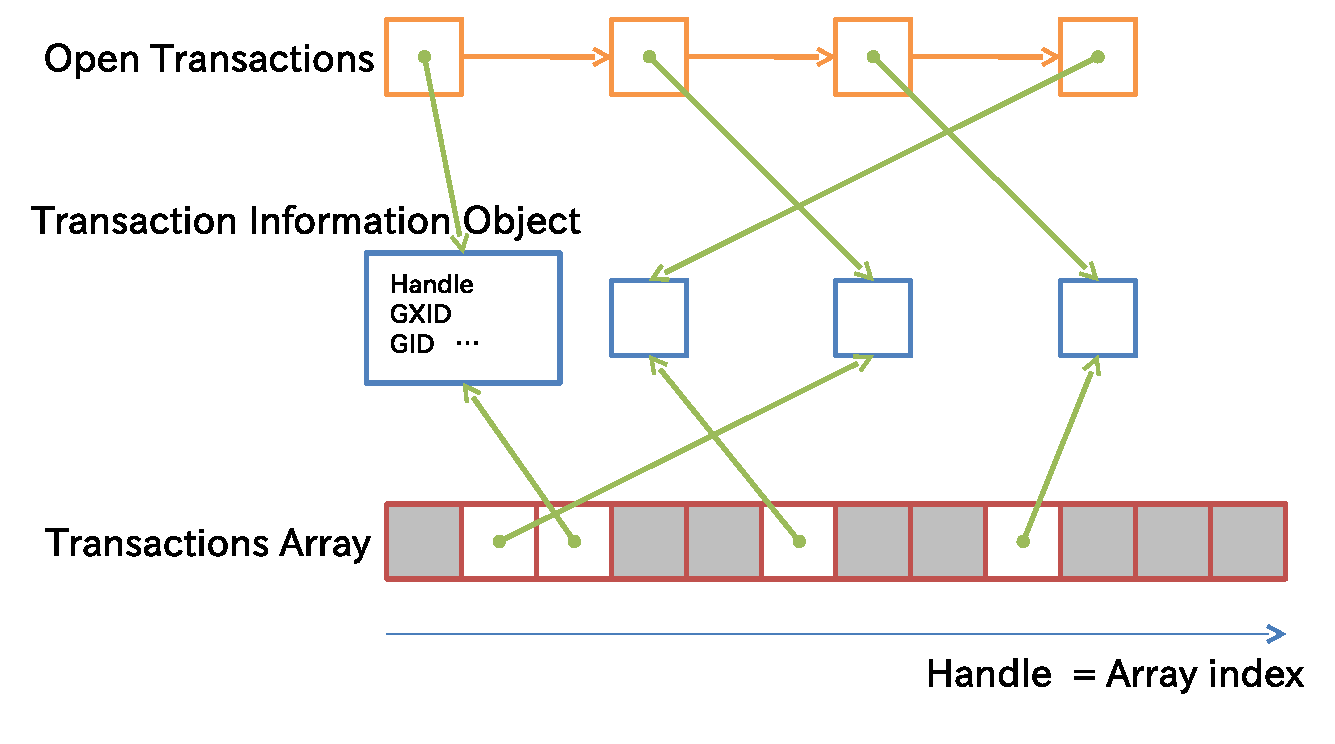
\includegraphics[width=0.8\hsize]{add_gtmtxn.eps}
		  \caption{\label{fig:addgtmtxn}Transaction management in GTM}
	  \end{center}
  \end{figure}
  
  Note: Some codes seems to be copied from \file{transam.c}.
  
  
  \FUNC{GTM\_HandleToTransactionInfo()}	%--------------------------------------
  
    Finds the corresponding transaction info structure by the transaction handle.
    %
    This is called from the following codes:
    
    \FuncRefHdr
		\FuncRef{-}{gtm_txn.c}{
		  \vspace{3pt}
		}\\
		\FuncRef{GTM_GetTransactionSnapshot}{gtm_snap.c}{
		  Used in taking the transaction snapshot to check and store information with given handles.
		}\\ \hline
    \FuncRefTrailor
  
  \FUNC{GTM_GXIDToHandle()}	%--------------------------------------
  
	Finds the transaction handle corresponding to given GXID.
    %
    This is called from the following codes:
    
    \FuncRefHdr
		\FuncRef{-}{gtm_txn.c}{
		  \vspace{3pt}
		}\\
		\FuncRef{ProcessGetSnapshotCommand}{gtm_snap.c}{
			Used in processing \file{MSG_SNAPSHOT_GET} command to obtain the handle from given
			GXID for querying the transaction information.
		}\\
		\FuncRef{ProcessGetSnapshotCommandMulti}{gtm_snap.c}{
			Used in processing \file{MSG_SNAPSHOT_GET_MULTI} command to obtain the handle from
			given GXID for querying the transaction information.
		}\\ \hline
    \FuncRefTrailor
  
  \FUNC{GTM_GIDToHandle()}	%--------------------------------------
  
	Finds the transaction handle corresponding to the 
    given the GID (for a prepared transaction).
    %
    This function is used by only the functions in the same file.
  
  \FUNC{GTM_InitTxnManager()}	%--------------------------------------
  
    Initializes global variables of the transaction manager.
    %
    This is called from the following codes:
    
    \FuncRefHdr
		\FuncRef{BaseInit}{main.c}{
		  Used in start up sequence.
		}\\ \hline
    \FuncRefTrailor
  
  \FUNC{GTM_BeginTransaction()}	%--------------------------------------
  
    Begins a new transaction and return assigned handle.
    
    This function creates new transaction object and register it into opend transaction list.
    
    This is called from the following codes:
    
	{
		\footnotesize
		\FuncRefHdr
			\FuncRef{ProcessBeginTransactionCommand}{gtm_txn.c}{
			  Used in processing \file{MSG_TXN_BEGIN} message
			}\\
			\FuncRef{ProcessBeginTransactionGetGXIDCommand}{gtm_txn.c}{
			  Used in processing \file{MSG_TXN_BEGIN_GETGXID} message
			}\\
			\FuncRef{ProcessBeginTransactionGetGXIDAutovacuumCommand}{gtm_txn.c}{
			  Used in processing \file{MSG_TXN_BEGIN_GETGXID_AUTOVACUUM} message
			}\\
			\FuncRef{ProcessGetGIDDataTransactionCommand}{gtm_txn.c}{
			  Used in processing \file{MSG_TXN_GET_GID_DATA} message
			}\\ \hline
		\FuncRefTrailor
	}
  
  
  \FUNC{GTM_BeginTransactionMulti()}	%--------------------------------------
  
    Begins a new transactions and returns number of new transactions began.
    
    This function delegates internal logic to \file{GTM_BeginTransaction}.
    
    This is called from the following codes:
    
	{
		\footnotesize
		\FuncRefHdr
			\FuncRef{GTM_BeginTransaction}{gtm_txn.c}{
			  Delegates internal logic
			}\\
			\FuncRef{ProcessBeginTransactionGetGXIDCommandMulti}{gtm_txn.c}{
			  Used in processing \file{MSG_TXN_BEGIN_GETGXID_MULTI} message
			}\\ \hline
		\FuncRefTrailor
	}
  
  \FUNC{GTM_RollbackTransaction()}	%--------------------------------------
  
	  Rolls back a transaction by handle.
	  
	  This function delegates internal logic to \file{GTM_RollbackTransactionMulti}.
	  
	  This is called from the following codes:
	  
	  {
		  \footnotesize
		  \FuncRefHdr
			  \FuncRef{GTM_RollbackTransactionGXID}{gtm_txn.c}{
				Convert GXID to handle and delegates internal logic
			  }\\
			  \FuncRef{ProcessRollbackTransactionCommand}{gtm_txn.c}{
				Used in processing \file{MSG_TXN_ROLLBACK} / \file{MSG_BKUP_TXN_ROLLBACK} message
			  }\\ \hline
		  \FuncRefTrailor
	  }
  
  \FUNC{GTM_RollbackTransactionMulti()}	%--------------------------------------
  
    Rolls back transactions by handles.
    
    This function marks transactions as ``rollback in progress'' and removes them from opend transaction list.
    
    This is called from the following codes:
    
    \FuncRefHdr
		\FuncRef{GTM_RollbackTransaction}{gtm_txn.c}{
		  Delegates internal logic
		}\\
		\FuncRef{ProcessRollbackTransactionCommandMulti}{gtm_txn.c}{
		  Used in processing \file{MSG_TXN_ROLLBACK_MULTI} or \file{MSG_BKUP_TXN_ROLLBACK_MULTI} message
		}\\
		\hline
    \FuncRefTrailor
  
  \FUNC{GTM_RollbackTransactionGXID()}	%--------------------------------------
  
    Rolls back transaction by GXID
    
    This function converts GXID to the handle and delegates internal logic to  \file{GTM_RollbackTransaction}.
    
    This function is never used.
  
  \FUNC{GTM_CommitTransaction()}	%--------------------------------------
  
    Commits a transaction by handle.
    
    This function delegates internal logic to \file{GTM_CommitTransactionMulti}.
    
    This is called from the following codes:
    
    \FuncRefHdr
		\FuncRef{GTM_CommitTransactionGXID}{gtm_txn.c}{
		  Convert GXID to handle and delegates internal logic
		}\\
		\FuncRef{ProcessCommitTransactionCommand}{gtm_txn.c}{
		  Used in processing \file{MSG_TXN_COMMIT} message
		}\\ \hline
    \FuncRefTrailor
  
  \FUNC{GTM_CommitTransactionMulti()}	%--------------------------------------
  
    Commits transactions by handles.
    
    This function marks transactions as ``commit in progress'' and removes them from opend transaction list.
    
    This is called from the following codes:

	{
		\footnotesize
		\FuncRefHdr
			\FuncRef{GTM_CommitTransaction}{gtm_txn.c}{
			  Delegates internal logic
			}\\
			\FuncRef{ProcessCommitPreparedTransactionCommand}{gtm_txn.c}{
			  Used in processing \file{MSG_TXN_COMMIT_PREPARED} / \file{MSG_BKUP_TXN_COMMIT_PREPARED} message
			}\\
			\FuncRef{ProcessCommitTransactionCommandMulti}{gtm_txn.c}{
			  Used in processing \file{MSG_TXN_COMMIT_MULTI} / \file{MSG_BKUP_TXN_COMMIT_MULTI} message
			}\\ \hline
		\FuncRefTrailor
	}
  
  \FUNC{GTM_CommitTransactionGXID()}	%--------------------------------------
  
    Commits a transaction by GXID.
    
    This function converts GXID to the handle and delegates internal logic to  \file{GTM_CommitTransaction}.
    
    This function is not used at present.
  
  \FUNC{GTM_PrepareTransaction()}	%--------------------------------------
  
    Prepares a transaction by the handle.
    
    This function marks transaction as ``prepared''.
    
    This is called from the following codes:
    
	{
		\footnotesize
		\FuncRefHdr
			\FuncRef{ProcessPrepareTransactionCommand}{gtm_txn.c}{
			  Used in processing \file{MSG_TXN_PREPARE} / \file{MSG_BKUP_TXN_PREPARE} message
			}\\ \hline
		\FuncRefTrailor
	}
  
  \FUNC{GTM_StartPreparedTransaction()}	%--------------------------------------
  
    Starts to prepare a transaction by the handle.
    
    This function save GID and marks transactions as ``prepare in progress''.
    
    This is called from the following codes:
    
	{
		\footnotesize
		\FuncRefHdr
			\FuncRef{GTM_StartPreparedTransactionGXID}{gtm_txn.c}{
			  Converts GXID to the handle and delegates internal logic
			}\\
			\FuncRef{ProcessStartPreparedTransactionCommand}{gtm_txn.c}{
			  Used in processing \file{MSG_TXN_START_PREPARED} / \file{MSG_BKUP_TXN_START_PREPARED} message
			}\\ \hline
		\FuncRefTrailor
	}
  
  \FUNC{GTM_StartPreparedTransactionGXID()}	%--------------------------------------
  
    Starts to prepare a transaction by GXID.
    
    This function converts GXID to the handle and delegates internal logic to  \file{GTM_StartPreparedTransaction}.
    
    This function is not used at present.
  
  \FUNC{GTM_GetGIDData()}	%--------------------------------------
  
    Gets information of a prepared transaction.
    %
    This is called from the following codes:
    
	{
		\footnotesize
		\FuncRefHdr
			\FuncRef{ProcessGetGIDDataTransactionCommand}{gtm_txn.c}{
			  Used in processing \file{MSG_TXN_GET_GID_DATA} message
			}\\ \hline
		\FuncRefTrailor
	}
  
  \FUNC{GTM_GetAllPrepared()}	%--------------------------------------
  
    \textbf{Not implemented yet}
  
  \FUNC{GTM_GetStatus()}	%--------------------------------------
  
    Gets transaction status.
    %
    This is called from the following codes:
    
    \FuncRefHdr
		\FuncRef{GTM_GetStatusGXID}{gtm_txn.c}{
		  Convert GXID to handle and delegates internal logic
		}\\
		\hline
    \FuncRefTrailor
  
  \FUNC{GTM_GetStatusGXID()}	%--------------------------------------
  
    Gets transaction status by GXID.
    
    This function converts GXID to handle and delegates internal logic to  \file{GTM_GetStatus}.
    
    This function is never used.
  
  \FUNC{GTM_GetAllTransactions()}	%--------------------------------------
  
    \textbf{Not implemented yet}
  
  \FUNC{GTM_RemoveAllTransInfos()}	%--------------------------------------
  
    Removes all the transaction information associated with the caller thread and the given backend.
    
    This function removes all the transaction information associated with the caller thread and the given backend from opened transaction list.
    This also calculates \texttt{latestCompletedXid}.
    
    This function is used to clear implicitly aborted transactions when a backend or a GTM proxy disconnect without committing, aborting and preparing.
    
    This is called from the following codes:
    
    \FuncRefHdr
		\FuncRef{GTM_ThreadMain}{main.c}{
		  Called when the message loop detected a backend disconnection.
		}\\
		\FuncRef{ProcessCommand}{main.c}{
		  Used in processing \file{MSG_BACKEND_DISCONNECT}
		}\\
		\hline
    \FuncRefTrailor


% - - - - subsubsection - - - - - - -  - - - - - - - - - - - - - - - - - - - - -

\subsubsection{gtm\_snap.c}

  This module supplies snapshot handling functions on GTM.
  
  \FUNC{GTM_GetSnapshotData()}	%--------------------------------------
  
    \textbf{Not implemented yet}
  
  \FUNC{GTM_GetTransactionSnapshot()}	%--------------------------------------
  
    Gets snapshot for the given transactions.
    
    This function takes transaction snapshots and saves to transaction information object.
    
    Although this function looks supporting \texttt{SERIALIZABLE} isolation level, the code is not complete.
    It doesn't a matter as long as \texttt{READ COMMITTED} isolation level is used.
    
    This is called from the following codes:
    
    \FuncRefHdr
		\FuncRef{ProcessGetSnapshotCommand}{gtm_snap.c}{
		  Used in processing \file{MSG_SNAPSHOT_GET}
		}\\
		\FuncRef{ProcessGetSnapshotCommandMulti}{gtm_snap.c}{
		  Used in processing \file{MSG_SNAPSHOT_GET_MULTI}
		}\\ \hline
    \FuncRefTrailor
  
  \FUNC{GTM_FreeCachedTransInfo()}	%--------------------------------------
  
    \textbf{Not implemented yet}
  
  \FUNC{GTM_BkupBeginTransactionMulti()}	%--------------------------------------
  
    Updates global transaction information to given ones.
    %
    This is called from the following codes:
    
    \FuncRefHdr
		\FuncRef{GTM_BkupBeginTransaction}{gtm_txn.c}{
		  Delegate internal logic
		}\\ \hline
    \FuncRefTrailor
  
  \FUNC{ProcessBeginTransactionCommandMulti()}	%--------------------------------------
  
    \textbf{Not implemented yet}
  
  
  \FUNC{GTM_SaveTxnInfo()}	%--------------------------------------
  
    Saves next GXID to the control file.
    %
    This is called from the following codes:
    
    \FuncRefHdr
		\FuncRef{GTM_MakeBackup}{gtm_backup.c}{
		  Used to save next GXID to the backup file
		}\\
		\FuncRef{ServerLoop}{main.c}{
		  Used in shutdown sequence
		}\\ \hline
    \FuncRefTrailor
  
  \FUNC{GTM_RestoreTxnInfo()}	%--------------------------------------
  
    Restores the next GXID from the control file.
    
    This function also sets \file{latestCompletedXid}.
    If the control file is not available, it uses given value
	from a \texttt{gtm} command line option.
    
    This is called from the following codes:
    
    \FuncRefHdr
		\FuncRef{gtm_standby_restore_next_gxid}{gtm_standby.c}{
		  \file{GTM_RestoreTxnInfo(NULL, next_gxid);}
		}\\
		\FuncRef{main}{main.c}{
		  Used in start up sequence
		}\\ \hline
    \FuncRefTrailor
  
  \FUNC{GTM_BkupBeginTransaction()}	%--------------------------------------
  
    Updates global transaction information to given one.
    
    This function delegates internal logic to  \file{GTM_BeginTransaction}.
    
    This is called from the following codes:
    
	{
		\footnotesize
		\FuncRefHdr
			\FuncRef{ProcessBkupBeginTransactionCommand}{gtm_txn.c}{
			  Used in processing \file{MSG_BKUP_TXN_BEGIN} message
			}\\ \hline
		\FuncRefTrailor
	}
  
  
  \FUNC{GTM_FreeSnapshotData()}	%--------------------------------------
  
    Releases the snapshot data
    
    This function releases the snapshot data.
    Please note that the snapshot itself is not freed by this function.
    
    This function is not used at present.



% - - - - subsubsection - - - - - - -  - - - - - - - - - - - - - - - - - - - - -

\subsubsection{\texttt{gtm\_seq.c}}

  This module supplies Sequence handling infrastructure.
  This is one of the most importarnt part of GTM.
  
  An instance of {\file{struct} \file{GTM_SeqInfo}} is created corresponding to a sequence in a database.
  The structure is shown in Table \ref{tab:gtmseqinfo}.
  Most of the member variables has corresponding \PG's sequence attribute.
  \file{gs_ref_count} is a GTM specific variable which manages reference to automatic
  destruction of the sequence, but there's no case that the sequence is destroyed by
  the reference count.
  
  The sequence information is stored into \file{GTMSequences} global hash table.
  Sequence information is distributed by the hash value of their name 
  so that character string comparison is not needed afterwords.
  
  \begin{table}[htp]
	  \begin{center}
		  \caption{\label{tab:gtmseqinfo}{Members of \texttt{struct GTM\_SeqInfo}}}\vspace{5pt}
		  \begin{tabular}{lp{0.6\hsize}} \hline
			Member variable & Description \\ \hline
			\file{gs_key} & Same as \file{sequence_name} of the sequence in \PG. \\
			\file{gs_value} & Same as \file{last_value} of the sequence in \PG. \\
			\file{gs_backedUpValue}
				& The last value of the sequence which is backuped to the control file. \\
			\file{gs_init_value} & Same as \file{start_value} of the sequence in \PG. \\
			\file{gs_last_value} & \textit{Updated but not used at present}. \\
			\file{gs_increment_by} & Same as \file{increment_bu} of the sequence in \PG. \\
			\file{gs_min_value} & Same as \file{min_value} of the sequence in \PG. \\
			\file{gs_max_value} & Same as \file{max_value} of the sequence in \PG. \\
			\file{gs_cycle} & Same as \file{is_cycled} of the sequence in \PG. \\
			\file{gs_called} & Same as \file{is_called} of the sequence in \PG. \\
			\file{gs_ref_count} & The reference count of the sequence object. \\
			\file{gs_state} & The state of the sequence. This variable could take
							  \file{SEQ_STATE_ACTIVE | SEQ_STATE_DELETED}.\\
			\file{gs_lock} & The lock for the sequence object.\\
			\hline
		  \end{tabular}
	  \end{center}
  \end{table}
  
  
  \FUNC{GTM_InitSeqManager()}	%--------------------------------------
  
    Initializes global variable for the sequence manager.
    %
    This is called from the following codes:
    
    \FuncRefHdr
		\FuncRef{BaseInit}{main.c}{
		  Used in start up sequence
		}\\ \hline
    \FuncRefTrailor
  
  \FUNC{GTM_SeqOpen()}	%--------------------------------------
  
    Initializes a new sequence.
    
    This function initializes a new sequence.
    Optionally set the initial value of the sequence.
    
    This is called from the following codes:
    
    \FuncRefHdr
		\FuncRef{ProcessSequenceInitCommand}{gtm_seq.c}{
		  Used in processing \file{MSG_SEQUENCE_INIT} message
		}\\ \hline
    \FuncRefTrailor
  
  \FUNC{GTM_SeqAlter()}	%--------------------------------------
  
    Alter a sequence.
    
    This function alternates current sequence parameters and given one.
    This function can't rename the sequence.
    
    This is called from the following codes:
    
    \FuncRefHdr
		\FuncRef{ProcessSequenceAlterCommand}{gtm_seq.c}{
		  Used in processing Process \file{MSG_SEQUENCE_ALTER} / \file{MSG_BKUP_SEQUENCE_ALTER} / \file{MSG_BKUP_SEQUENCE_ALTER} message
		}\\ \hline
    \FuncRefTrailor
  
  \FUNC{GTM_SeqClose()}	%--------------------------------------
  
    Destroys the given sequence depending on the type of given key
    
    This function can take a sequence name or a database name.
    If a sequence name is given, it destroys the sequence.
    If database name is given, it destroys all of the sequences belogs to the database using prefix of full quolified sequence name.
    Latter functionarity is used when dropping a database.
    
    This is called from the following codes:
    
    \FuncRefHdr
		\FuncRef{GTM_SeqRename}{gtm_seq.c}{
		  Used in renaming sequence to destroy old sequence info.
		}\\
		\FuncRef{ProcessSequenceCloseCommand}{gtm_seq.c}{
		  Used in processing \file{MSG_SEQUENCE_CLOSE} / \file{MSG_BKUP_SEQUENCE_CLOSE} / \file{MSG_BKUP_SEQUENCE_CLOSE} message
		}\\ \hline
    \FuncRefTrailor
  
  \FUNC{GTM_SeqRename()}	%--------------------------------------
  
    Rename an existing sequence with a new name
    
    This function creates a new sequence object and copies parameters from old one,
	which is destroyed then.
    
    This is called from the following codes:
    
    \FuncRefHdr
		\FuncRef{ProcessSequenceRenameCommand}{gtm_seq.c}{
		  Used in processing \file{MSG_SEQUENCE_RENAME} / \file{MSG_BKUP_SEQUENCE_RENAME} / \file{MSG_BKUP_SEQUENCE_RENAME} message
		}\\ \hline
    \FuncRefTrailor
  
  \FUNC{GTM_SeqGetNext()}	%--------------------------------------
  
    Gets the next value for the sequence.
    %
    This is called from the following codes:
    
    \FuncRefHdr
		\FuncRef{ProcessSequenceGetNextCommand}{gtm_seq.c}{
		  Used in processing \file{MSG_SEQUENCE_GET_NEXT} / \file{MSG_BKUP_SEQUENCE_GET_NEXT} / \file{MSG_BKUP_SEQUENCE_GET_NEXT} message.
		}\\ \hline
    \FuncRefTrailor
  
  \FUNC{GTM_SeqSetVal()}	%--------------------------------------
  
    Sets values for the sequence.
    %
    This is called from the following codes:
    
    \FuncRefHdr
		\FuncRef{ProcessSequenceSetValCommand}{gtm_seq.c}{
		  Used in processing \file{MSG_SEQUENCE_SET_VAL} / \file{MSG_BKUP_SEQUENCE_SET_VAL} /
		  \file{MSG_BKUP_SEQUENCE_SET_VAL} message.
		}\\ \hline
    \FuncRefTrailor
  
  \FUNC{GTM_SeqReset()}	%--------------------------------------
  
    Resets the sequence.
    %
    This is called from the following codes:
    
    \FuncRefHdr
		\FuncRef{ProcessSequenceResetCommand}{gtm_seq.c}{
		  Used in processing \file{MSG_SEQUENCE_RESET} / \file{MSG_BKUP_SEQUENCE_RESET} /
		  \file{MSG_BKUP_SEQUENCE_RESULT} message.
		}\\ \hline
    \FuncRefTrailor
  
  \FUNC{GTM_SaveSeqInfo()}	%--------------------------------------
  
    Saves all the sequence information.
    
    This is called from the following codes:
    
    \FuncRefHdr
		\FuncRef{GTM_MakeBackup}{gtm_backup.c}{
		  Used in making a backup file.
		  This function is never used.
		}\\
		\FuncRef{ServerLoop}{main.c}{
		  Used in shutting down sequence to save sequence information for next run.
		}\\ \hline
    \FuncRefTrailor
  
  \FUNC{GTM_RestoreSeqInfo()}	%--------------------------------------
  
    Restores sequence information from the control file.
    
	\begin{itemize}
		\item This function is used only by the functions in the same file.
		\item This is also called from the following codes:
	\end{itemize}
    
    \FuncRefHdr
		\FuncRef{main}{main.c}{
		  \file{GTM_RestoreSeqInfo(ctlf);}`
		}\\
		\hline
    \FuncRefTrailor
  
  \FUNC{GTM_SeqRestore()}	%--------------------------------------
  
    Restores a sequence.
    %
    This is called from the following codes:
    
    \FuncRefHdr
		\FuncRef{GTM_RestoreSeqInfo}{gtm_seq.c}{
		  Used in restoring sequences information from a file, which is typically the control file
		}\\
		\FuncRef{gtm_standby_restore_sequence}{gtm_standby.c}{
		  Used in restoring sequences information from a GTM master
		}\\ \hline
    \FuncRefTrailor
  
  \FUNC{GTM_NeedSeqRestoreUpdate()}	%--------------------------------------
  
    Tests if backup data needs update after the given sequence is touched.
    
    This function is not used at present.
  
  \FUNC{GTM_WriteRestorePointSeq()}	%--------------------------------------
  
    Writes the restoration point of all the sequences.
    
    This function saves restore point of all sequences to the file, which is typically the control file.
    The restore point is saved to deal with abnormal termination of GTM, they are advanced 2000 count to
	current value at maximum to avoid frequent disk write.
    
    This is called from the following codes:
    
    \FuncRefHdr
		\FuncRef{GTM_WriteRestorePoint}{gtm_backup.c}{
		  Used in making the control file to write sequences information
		}\\
		\FuncRef{GTM_WriteBarrierBackup}{gtm_backup.c}{
		  Used in making a barrier file to write sequences information
		}\\ \hline
    \FuncRefTrailor



% - - - - subsubsection - - - - - - -  - - - - - - - - - - - - - - - - - - - - -

\subsubsection{\texttt{gtm\_thread.c}}

  This module supplies thread handling functions.
  
  The things to note here is thread-specific data is stored in \file{GTM_ThreadInfo}
  structure.
  It is allocated in thread-local storage and we can access it using \file{GetMyThreadInfo} macro.
  \file{GetMyThreadInfo} uses pthread function to obtain the pointer and the key
  \file{threadinfo_key} is created in \file{main.c} and \file{main_proxy.c}.
  
  \file{MyPort} macro is implicitly used in libpq functions to determine what connection to use.
  This macro is redefined in GTM to refer to variables in thread-specific data.
  This change reduces much effort to port libpq into thread model.
  
  Memory contexts are similar to the case of \file{MyPort}.
  Many memory contexts such as \file{TopMemoryContext}, \file{ErrorContext}, \file{MessageContext} and
  \file{CurrentMemoryContext}, are stored in \file{GTM_ThreadInfo} for each thread and
  corresponding macros are also redefined.
  All of the memory allocated with these context are freed by thread cleanup function when the thread exits.
  
  \FUNC{GTM_ThreadAdd()}	%--------------------------------------
  
    Adds the given thrinfo structure to the global array.
    
    This function adds the given thrinfo structure to the global array.
    If the array is full, it expands it automatically.
    
    This is called from the following codes:
    
    \FuncRefHdr
		\FuncRef{GTM_ThreadCreate}{gtm_thread.c}{
		  Used in creating a new thread for a GTM client.
		}\\
		\FuncRef{BaseInit}{main.c}{
		  Used in the initialization of the main thread.
		}\\ \hline
    \FuncRefTrailor
  
  \FUNC{GTM_ThreadRemove()}	%--------------------------------------
  
    Removes given \file{GTM_ThreadInfo} structure from the global array.
    
    This is called from the following codes:
    
    \FuncRefHdr
		\FuncRef{GTM_ThreadCleanup}{gtm_thread.c}{
		  Used in cleaning up of a thread
		}\\ \hline
    \FuncRefTrailor
  
  \FUNC{GTM_ThreadJoin()}	%--------------------------------------
  
    Waits for exitting of given thread.
    
    This function is not used at present.
  
  \FUNC{GTM_ThreadExit()}	%--------------------------------------
  
    Exits this thread immediately.
    
    This function is not used at present.
  
  \FUNC{GTM_LockAllOtherThreads()}	%--------------------------------------
  
    Locks all the thread information objects of all other threads.
    
    This function is not used at present.
  
  \FUNC{GTM_UnlockAllOtherThreads()}	%--------------------------------------
  
    Unlocks all the information objects of all the other threads.
    
    This function is not used at present.
  
  \FUNC{GTM_DoForAllOtherThreads()}	%--------------------------------------
  
    Invokes callback function function for each of other thread information objects.
    %
    This is called from the following codes:
    
    \FuncRefHdr
		\FuncRef{ProcessPGXCNodeRegister}{register_gtm.c}{
		  Used in processing \file{MSG_NODE_REGISTER} message to disconnect connections to GTM slave in all threads when new GTM standby is registered.
		}\\ \hline
    \FuncRefTrailor
  
  \FUNC{GTM_ThreadCreate()}	%--------------------------------------
  
    Creates a new thread and assigns the given connection to it.
    
    This function creates a new thread, thread local memory contexts and a thread information object, and assign the given connection to the thread.
    
    This is called from the following codes:
    
    \FuncRefHdr
		\FuncRef{GTMAddConnection}{main.c}{
		  Used in adding new connection from a GTM client.
		}\\ \hline
    \FuncRefTrailor
  
  \FUNC{GTM_GetThreadInfo()}	%--------------------------------------
  
    \textit{Not implemented yet.}
  
  

% - - - - subsubsection - - - - - - -  - - - - - - - - - - - - - - - - - - - - -

\subsubsection{\texttt{gtm\_backup.c}}
  
  This module supplies backup functions on GTM.
  
  \FUNC{GTM_WriteRestorePoint()}	%--------------------------------------
  
    Writes restoration point.
    
    This function saves restoration point of GXID and sequences to the control file.
    The restore point is saved to deal with abnormal termination of GTM.
   	They are advanced 2000 count to current value at maximum.
    
    This is called from the following codes:
    
    \FuncRefHdr
		\FuncRef{main}{main.c}{
		  Used in start up sequence after all the data are restored.
		}\\
		\FuncRef{ProcessCommand}{main.c}{
		  Used in main loop when backup is needed.
		}\\
		\FuncRef{PromoteToActive}{main.c}{
		  Used in promoting to activate.
		}\\ \hline
    \FuncRefTrailor
  
  \FUNC{GTM_MakeBackup()}	%--------------------------------------
  
    Saves the next GXID and sequence information to given backup file.
    
    This function is not used at present.
  
  \FUNC{GTM_SetNeedBackup()}	%--------------------------------------
  
    Set \textbf{need backup} flag to true
    
    This function sets \textbf{need backup} flag to true.
    This flag means transaction or sequence information are need to be saved.
    
    This is called from the following codes:
    
    \begin{itemize}
      \item When the sequence value is created or jumped or removed.
      \item When the sequence value is incremented and it catches up with backed-up value.
      \item When GXID is incremented and it catches up with backed-up value.
    \end{itemize}
  
  \FUNC{GTM_NeedBackup()}	%--------------------------------------
  
    Tests \textbf{need backup} flag.
    %
    This is called from the following codes:
    
    \FuncRefHdr
		\FuncRef{ProcessCommand}{main.c}{
		  Used in message loop to decide whether do backup or not.
		}\\ \hline
    \FuncRefTrailor
  
  \FUNC{GTM_WriteBarrierBackup()}	%--------------------------------------
  
    Creates GTM restration point file corresponding to a barrier.
    %
    This is called from the following codes:
    
    \FuncRefHdr
		\FuncRef{ProcessBarrierCommand}{main.c}{
		  Used in processing \file{MSG_BARRIER} / \file{MSG_BKUP_BARRIER} message
		}\\ \hline
    \FuncRefTrailor



% - - - - subsubsection - - - - - - -  - - - - - - - - - - - - - - - - - - - - -

\subsubsection{\texttt{gtm\_standby.c}}

  This module supplies functionalities of GTM Standby.
  
  \FUNC{gtm_is_standby()}	%--------------------------------------
  
    \textbf{Not implemented yet.}
  
  \FUNC{gtm_set_standby()}	%--------------------------------------
  
    \textbf{Not implemented yet.}
  
  \FUNC{gtm_set_active_conninfo()}	%--------------------------------------
  
    \textbf{Not implemented yet.}
  
  \FUNC{gtm_standby_start_startup()}	%--------------------------------------
  
    Initializes GTM standby startup.
    
    This function connects to GTM active and initialize locks for standby mode.
    
    This is called from the following codes:
    
    \FuncRefHdr
		\FuncRef{main}{main.c}{
		  Used in start up sequence of GTM standby
		}\\ \hline
    \FuncRefTrailor
  
  \FUNC{gtm_standby_finish_startup()}	%--------------------------------------
  
    Finishes GTM standby startup
    
    This function closes connection to GTM active for connect-back from master.
    
    This is called from the following codes:
    
    \FuncRefHdr
		\FuncRef{main}{main.c}{
		  Used in start up sequence of GTM standby
		}\\ \hline
    \FuncRefTrailor
  
  \FUNC{gtm_standby_restore_next_gxid()}	%--------------------------------------
  
    Gets the next GXID value from GTM active.
    %
    This is called from the following codes:
    
    \FuncRefHdr
		\FuncRef{main}{main.c}{
		  Used in start up sequence of GTM standby
		}\\ \hline
    \FuncRefTrailor
  
  \FUNC{gtm_standby_restore_gxid()}	%--------------------------------------
  
    Restores global transaction information from GTM active.
    %
    This is called from the following codes:
    
    \FuncRefHdr
		\FuncRef{main}{main.c}{
		  Used in start up sequence of GTM standby
		}\\ \hline
    \FuncRefTrailor
  
  \FUNC{gtm_standby_restore_sequence()}	%--------------------------------------
  
    Restores sequence information from GTM active.
    %
    This is called from the following codes:
    
    \FuncRefHdr
		\FuncRef{main}{main.c}{
		  Used in start up sequence of GTM standby
		}\\ \hline
    \FuncRefTrailor
  
  \FUNC{gtm_standby_restore_node()}	%--------------------------------------
  
    Restores node information from GTM active.
    %
    This is called from the following codes:
    
    \FuncRefHdr
		\FuncRef{main}{main.c}{
		  Used in start up sequence of GTM standby
		}\\ \hline
    \FuncRefTrailor
  
  \FUNC{gtm_standby_register_self()}	%--------------------------------------
  
    Registers itself to the GTM active as a ``disconnected'' node.
    
    This function registers myself to the GTM active as a ``disconnected'' node before restore starts.
    This status would be updated later after restoring completion.
    
    This function's comment saids above, but \file{PorcessPGXCNodeRegister()} which processes \file{MSG_NODE_REGISTER} message ignores the status ``disconnected''.
    
    This is called from the following codes:
    
    \FuncRefHdr
		\FuncRef{main}{main.c}{
		  Used in start up sequence of GTM standby
		}\\ \hline
    \FuncRefTrailor
  
  \FUNC{gtm_standby_activate_self()}	%--------------------------------------
  
    Update node status of itself from "disconnected" to "connected" in GTM active.
    
    This function unregisters myself once, after that it registers myself again as ``connected'' node.
    
    This is called from the following codes:
    
    \FuncRefHdr
		\FuncRef{main}{main.c}{
		  Used in start up sequence of GTM standby
		}\\ \hline
    \FuncRefTrailor
  
  \FUNC{gtm_standby_connect_to_standby()}	%--------------------------------------
  
    Makes a connection to the GTM standby.
    
    This is called from the following codes:
    
    \FuncRefHdr
		\FuncRef{ServerLoop}{main.c}{
		  Used in GTM active accept loop when a GTM client connected.
		}\\
		\FuncRef{GTM_ThreadMain}{main.c}{
		  Used in GTM active message loop when a GTM slave newly registered.
		}\\ \hline
    \FuncRefTrailor
  
  \FUNC{gtm_standby_disconnect_from_standby()}	%--------------------------------------
  
    Disconnects connection from GTM standby.
    
    This function disconnects given connection if it is not in standby mode.
    
    This is called from the following codes:
    
    \FuncRefHdr
		\FuncRef{gtm_standby_reconnect_to_standby}{gtm_standby.c}{
		  Used in reconnection to GTM standby to close old connection.
		}\\
		\FuncRef{ServerLoop}{main.c}{
		  Used in accept loop to cancel connection to GTM standby when GTM can't accept more connection.
		}\\
		\FuncRef{GTM_ThreadMain}{main.c}{
		  Used in message loop to close existing connection to GTM standby when GTM standby is unregistered.
		}\\ \hline
    \FuncRefTrailor
  
  \FUNC{gtm_standby_reconnect_to_standby()}	%--------------------------------------
  
    Reconnects to GTM standby.
    
    This function closes old connection and reconnects to GTM standby if it is not in standby mode.
    
    This is called from the following codes:
    
    \FuncRefHdr
		\FuncRef{gtm_standby_check_communication_error}{gtm_standby.c}{
		  Used in checking communication error with standby when it detects an error.
		}\\ \hline
    \FuncRefTrailor
  
  \FUNC{gtm_standby_check_communication_error()}	%--------------------------------------
  
    Checks if communication with standby made an error.
    
    This function checks whether the communication with standby made an error.
	If an error is detected, it reconnects to GTM standby.
    
    This is called from everywhere which makes interaction with GTM standby.
  
  \FUNC{find_standby_node_info()}	%--------------------------------------
  
    Finds ``one'' GTM standby node info.
    
    This function returns node information of GTM standby.
    Please note that GTM cannot have multiple GTM standby nodes.
    
    This is called from the following codes:
    
    \FuncRefHdr
		\FuncRef{gtm_standby_connect_to_standby_int}{gtm_standby.c}{
		  Used in connecting to GTM standby
		}\\
		\FuncRef{ProcessPGXCNodeRegister}{register_gtm.c}{
		  Used in processing \file{MSG_NODE_REGISTER} message to check the standby node has not been registered yet.
		}\\ \hline
    \FuncRefTrailor
  
  \FUNC{gtm_standby_begin_backup()}	%--------------------------------------
  
    Notifies GTM standby is beginning backup of GTM active.
    %
    This is called from the following codes:
    
    \FuncRefHdr
		\FuncRef{main}{main.c}{
		  Used in start up sequence of GTM standby
		}\\ \hline
    \FuncRefTrailor
  
  \FUNC{gtm_standby_end_backup()}	%--------------------------------------
  
    Notifies GTM standby is ending backup of GTM active.
    %
    This is called from the following codes:
    
    \FuncRefHdr
		\FuncRef{main}{main.c}{
		  Used in start up sequence of GTM standby
		}\\ \hline
    \FuncRefTrailor
  
  \FUNC{gtm_standby_closeActiveConn()}	%--------------------------------------
  
    \textit{Not implemented yet.}
  
  \FUNC{gtm_standby_finishActiveConn()}	%--------------------------------------
  
    Unregisters itself from GTM active.
    
    This function is not used at present.
  
  \FUNC{ProcessGTMBeginBackup()}	%--------------------------------------
  
    Handler of \file{MSG_BEGIN_BACKUP}.
    
    This function sets thread status to \file{GTM_THREAD_BACKUP} and locks all of other thread information objects.
    This function also sends a result immediately to GTM standby.
    
    This is called from the following codes:
    
    \FuncRefHdr
		\FuncRef{ProcessCommand}{main.c}{
		  Used in processing \file{MSG_BEGIN_BACKUP}
		}\\ \hline
    \FuncRefTrailor
  
  \FUNC{ProcessGTMEndBackup()}	%--------------------------------------
  
    Processes \file{MSG_END_BACKUP}.
    
    This function resets thread status to \file{GTM_THREAD_RUNNING} from \file{GTM_THREAD_BACKUP} and unlocks all of other thread information objects.
    This function also sends a result immediately to GTM standby.
    
    This is called from the following codes:
    
    \FuncRefHdr
		\FuncRef{ProcessCommand}{main.c}{
		  Used in processing \file{MSG_END_BACKUP}
		}\\ \hline
    \FuncRefTrailor


% - - - - subsubsection - - - - - - -  - - - - - - - - - - - - - - - - - - - - -

\subsubsection{\texttt{gtm\_time.c}}

  This module supplies timestamp handling functions on GTM.
  
  \FUNC{GTM_TimestampGetCurrent()}	%--------------------------------------
  
    Gets the current timestamp.
    %
    This is called from the following codes:
    
	{
		\footnotesize
		\FuncRefHdr
			\FuncRef{ProcessBeginTransactionCommand}{gtm_txn.c}{
			  Used to get transaction start timew
			}\\
			\FuncRef{ProcessBeginTransactionGetGXIDCommand}{gtm_txn.c}{
			  Used to get transaction start timew
			}\\
			\FuncRef{ProcessBeginTransactionGetGXIDCommandMulti}{gtm_txn.c}{
			  Used to get transaction start timew
			}\\ \hline
		\FuncRefTrailor
	}



% - - - - subsubsection - - - - - - -  - - - - - - - - - - - - - - - - - - - - -

\subsubsection{\texttt{replication.c}}

  This module supplies controlling the initialization and end of replication process of GTM data.
  These function is implemented but never used in \XC, so explanations are omitted.



% - - - - subsubsection - - - - - - -  - - - - - - - - - - - - - - - - - - - - -

\subsubsection{\texttt{gtm\_stat.c}}

  This module is not implemented yet.



% - - - - subsubsection - - - - - - -  - - - - - - - - - - - - - - - - - - - - -

\subsubsection{\texttt{gtm\_stats.c}}

  This module is not implemented yet.



%------- Subsec Subsec -----------------------------------------------------

\subsection{Configuration Modules}

  Since many part of configuration related functions seem to be copied from \PG{} and these are not point of the GTM.
  The explanations of these files listed in Table \ref{tab:omitgtmconf} are omitted.
  
  \begin{table}[htp]
	  \begin{center}
	  \caption{\label{tab:omitgtmconf}Source files related to configuration}\vspace{5pt}
		  \begin{tabular}{l} \hline
			  Path \\ \hline
			  \file{src/gtm/main/gtm_opt.c} \\
			  \file{src/gtm/config/gtm_opt_handler.c} \\
			  \file{src/gtm/config/gtm_opt_scanner.l} \\
			   \hline
		  \end{tabular}
	  \end{center}
  \end{table}




%
% ---- GTM Proxy ---------------------
%

%========= SECTION SECTION ===================================================

\section{\label{sec:gtmProxy}GTM Proxy}


  This module supplies proxy function of GTM to reduce the network traffic to GTM.
  Please refer to section \ref{arch:5_2} for the functional details.
  
  GTM Proxy is implemented as a independent process to the postmaster and the GTM.
  It means that GTM Proxy has its own binary, configuration file, log file and pid file, and we need to start the process separately.
  
  Many codes are shared with GTM, and codes specific only to GTM Proxy are described here.
  

%------- Subsec Subsec -----------------------------------------------------

\subsection{Utility functions}
  

% - - - - subsubsection - - - - - - -  - - - - - - - - - - - - - - - - - - - - -

\subsubsection{\texttt{proxy\_utils.c}}
  
  This module provides utility functions in GTM Proxy.
  
  \FUNC{gtm_standby_check_communication_error()}	%--------------------------------------
  
    No operation.
    
    This function is a dummy function of GTM Proxy to avoid object link problem.
    
    Most of command processing functions are existing only in GTM, but a few are both in
	GTM and GTM Proxy, which consist of same binary objects.
    All the command processing functions require calling
    \file{gtm_standby_check_communication_error()} for GTM.



%------- Subsec Subsec -----------------------------------------------------

\subsection{Main Program}


% - - - - subsubsection - - - - - - -  - - - - - - - - - - - - - - - - - - - - -

\subsubsection{\texttt{proxy\_main.c}}

  This file contains main module to run GTM Proxy process.
  
  The GTM Proxy is initialized as following sequence in \file{main()}.
  It's very simple: Setup configuration, initialize the main thread, restore information from
  files, create worker threads and accept connections.
  
  {\newcommand{\DA}{\textdownarrow}
  	\begin{center}
  	%\ovalbox{
  	\fbox{
  		\parbox{0.6\hsize}{
  			\center
  			\file{InitializeGTMOptions()} \\ \DA\\
  			\textit{(Parse command line options and load configuration file)} \\ \DA\\
  			\file{BaseInit()} \\ \DA\\
  			\file{GTM_Recovery_RestoreRegisterInfo()} \\ \DA\\
  		    \textit{(Establish input sockets)} \\ \DA\\
  			\textit{(Setup signal handlers)} \\ \DA\\
  			\textit{(Create worker threads)} \\ \DA\\
  			\file{ServerLoop()}
  		}
  	}
  	\end{center}
  }
  
  \file{ServerLoop()} is brought from same name function of \file{postmaster.c}.
  It registers itself to GTM, waits for new connections and calls \file{GTMProxyAddConnection()}
  to assign them to worker threads.
  If it detects a signal to abort, the process just exits.
  
  \file{GTMProxy_ThreadMain()} is a main function and includes the message loop.
  This function seems to be copied from \file{postmaster.c:BackendRun()}.
  First it initializes many things such as a memory context, the connection to GTM,
  buffer strings and an exception stack.
  As in the case of \PG{}, a signal and an error in child functions is notified with long jump, so
  an exception handler is registered using \file{sigsetjmp()}.
  But the long jump is allowed in very narrow block in \file{GTMProxy_ThreadMain} because
  a worker thread handles multiple backends and handles multiple message simultaneously.
  The block allowed to jump is surrounded \file{Enable_Longjmp()} and \file{Disable_Longjmp()}
  
  \file{GTM_ThreadMain()} reads messages from backends with \file{ReadCommand()} and calls
  \file{ProcessCommand()} for each message to process the ``command'' message from GTM clients.
  \file{ProcessCommand()} dispatches the message as shown in Table \ref{tab:gtmpxyproc}.
  The processing function dispatched a command message processes the message.
  Most of the messages are passed to GTM as is, with a proxy header using
  \file{GTMProxy_ProxyCommand()}.
  Some messages are pended to pack into single message using \file{GTMProxy_CommandPending()},
  and \file{GTMProxy_ProcessPendingCommands()} called after all of the backends are read and
  handled by \file{ProcessCommand()} which handles these pended messages.
  Exceptions are messages \file{MSG_NODE_REGISTER} and \file{MSG_NODE_UNREGISTER}.
  These messages are passed to GTM with the host name of the GTM Proxy using
  \file{GTMProxy_ProxyPGXCNodeCommand()}.
  So the proxy functions just put the message into libpq buffer.
  After all messages are ready to send, GTM Proxy append \file{MSG_DATA_FLUSH} message that
  has type ``F'' and flush the buffer.
  
  The messages sent by the proxy functions are stored into a linked list, GTM Proxy handles
  the response for each message in the list.
  The response is read from GTM with \file{GTMPQgetResult()}, and it is handled by
  \file{ProcessResponse()}.
  \file{ProcessResponse()} finds appropriate connection to the sent message and sends back the
  response message.
  If the sent message is packed message, unpacks it and sends corresponding response to
  each backend.
  
  If the message loop detects disconnection of a backend, it sends \file{MSG_BACKEND_DISCONNECT}
  message to GTM with \file{GTMProxy_CommandPending()}.
  The connection information is removed from the thread after the end of the message loop.
  
  In an opposite case that a new connection is assigned to the thread, the connection handshaked and
  reading socket array is reconstructed at the beginning of the message loop.
  It means that there's no traffic in existing connection, the new connection spoils one
  second passes at maximum.
  
  {
	  \scriptsize
	  \begin{longtable}{p{0.25\hsize}ll}
		  \caption{\label{tab:gtmpxyproc}GTM Proxy message processing functions} \\
		  \hline
		  Message & Processing function & Proxy function \\ \hline
		  \file{MSG_NODE_REGISTER} & \file{ProcessPGXCNodeCommand()} & \file{GTMProxy_ProxyPGXCNodeCommand()} \\
		  \file{MSG_NODE_UNREGISTER} & & \file{GTMProxy_ProxyPGXCNodeCommand()} \\
		  \hline
		  \file{MSG_TXN_BEGIN_GETGXID} & \file{ProcessTransactionCommand()} & \file{GTMProxy_CommandPending()} \\
		  \file{MSG_TXN_COMMIT} & & \file{GTMProxy_CommandPending()} \\
		  \file{MSG_TXN_ROLLBACK} & & \file{GTMProxy_CommandPending()} \\
		  \file{MSG_TXN_BEGIN} & & {\it Not supported} \\
		  \file{MSG_TXN_GET_GXID} & & {\it Not supported} \\
		  \file{MSG_TXN_BEGIN_GETGXID_AUTOVACUUM} & & \file{GTMProxy_ProxyCommand()} \\
		  \file{MSG_TXN_PREPARE} & & \file{GTMProxy_ProxyCommand()} \\
		  \file{MSG_TXN_START_PREPARED} & & \file{GTMProxy_ProxyCommand()} \\
		  \file{MSG_TXN_GET_GID_DATA} & & \file{GTMProxy_ProxyCommand()} \\
		  \file{MSG_TXN_COMMIT_PREPARED} & & \file{GTMProxy_ProxyCommand()} \\
		  \hline
		  \file{MSG_SNAPSHOT_GET} & \file{ProcessSnapshotCommand()} & \file{GTMProxy_CommandPending()}\footnote{If the message does not allow grouping, \file{GTMProxy_ProxyCommand()} is called.} \\
		  \file{MSG_SNAPSHOT_GXID_GET} & & {\it Not supported} \\
		  \hline
		  \file{MSG_SEQUENCE_INIT} & \file{ProcessSequenceCommand()} & \file{GTMProxy_ProxyCommand()} \\
		  \file{MSG_SEQUENCE_ALTER} & & \file{GTMProxy_ProxyCommand()} \\
		  \file{MSG_SEQUENCE_GET_NEXT} & & \file{GTMProxy_ProxyCommand()} \\
		  \file{MSG_SEQUENCE_SET_VAL} & & \file{GTMProxy_ProxyCommand()} \\
		  \file{MSG_SEQUENCE_RESET} & & \file{GTMProxy_ProxyCommand()} \\
		  \file{MSG_SEQUENCE_CLOSE} & & \file{GTMProxy_ProxyCommand()} \\
		  \file{MSG_SEQUENCE_RENAME} & & \file{GTMProxy_ProxyCommand()} \\
		  \hline
		  \file{MSG_BARRIER} & \file{ProcessBarrierCommand()} & \file{GTMProxy_ProxyCommand()} \\
		  \hline
	  \end{longtable}
  }



% - - - - subsubsection - - - - - - -  - - - - - - - - - - - - - - - - - - - - -

\subsubsection{\texttt{proxy\_thread.c}}

  This module supplies thread handling function in GTM Proxy.
  This module is similar to \file{gtm_thread.c}, but please note that GTM Proxy doesn't create new thread per GTM client.
  GTM Proxy adopts worker thread model, a worker thread handles multiple backends.
  
  \FUNC{GTMProxy_ThreadAdd()}	%--------------------------------------
  
    Adds the given thrinfo structure to the global array
    
    This function adds the given thrinfo structure to the global array.
    If the array is full, it is expanded automatically.
    
    This is called from the following codes:
    
    \FuncRefHdr
		\FuncRef{GTMProxy_ThreadCreate}{proxy_thread.c}{
		  Used in creating new thread
		}\\
		\FuncRef{BaseInit}{proxy_main.c}{
		  Used in start up sequence to register the main thread.
		}\\ \hline
    \FuncRefTrailor
  
  \FUNC{GTMProxy_ThreadRemove()}	%--------------------------------------
  
    Removes the given thrinfo structure from the global array.
    
    This function is not used at present.
  
  \FUNC{GTMProxy_ThreadJoin()}	%--------------------------------------
  
    Waits given thread to exit.
    
    This function is not used at present.
  
  \FUNC{GTMProxy_ThreadExit()}	%--------------------------------------
  
    Exits this thread immediately.
    
    This function is not used at present.
  
  \FUNC{GTMProxy_ThreadCreate()}	%--------------------------------------
  
    Creates a new thread and assigns it to the given thread information slot.
    
    This function creates a new thread, thread local memory contexts and a thread information object,
	and then assigns the thread to the given thread information slot.
    
    Please note that the comment says that the function assigns connection to thread, it's bogus.
    
    This is called from the following codes:
    
    \FuncRefHdr
		\FuncRef{main}{proxy_main.c}{
		  Used in start up sequence to create worker threads.
		}\\ \hline
    \FuncRefTrailor
  
  \FUNC{GTMProxy_GetThreadInfo()}	%--------------------------------------
  
    \textit{Not implemented yet.}
  
  \FUNC{GTMProxy_ThreadAddConnection()}	%--------------------------------------
  
    Adds a connection to a worker thread.
    
    This function adds the given connection to the thread selected by a round-robin manner.
    The caller is responsible only for accepting the connection.
    Other things including the authentication is done by the worker thread when it finds a new entry in the connection list.
    
    This function also assigns the connection to the connection ID.
    It is thread local ID and it is distinct from index of the connection information array.
    
    This is called from the following codes:
    
    \FuncRefHdr
		\FuncRef{GTMProxyAddConnection}{proxy_main.c}{
		  Used in adding new connection from a GTM client.
		}\\ \hline
    \FuncRefTrailor
  
  \FUNC{GTMProxy_ThreadRemoveConnection()}	%--------------------------------------
  
    This function removes the given connection from the assignment of a worker thread.
    It chinks a gap in connection information array made by removing the connection.
    The index of connections may change.
    
    This function also releases the connection ID assigned to given connection.
    
    This is called from the following codes:
    
    \FuncRefHdr
		\FuncRef{GTMProxy_ThreadMain}{proxy_main.c}{
		  Used in the message loop when it detects disconnection of a GTM client.
		}\\ \hline
    \FuncRefTrailor



% - - - - subsubsection - - - - - - -  - - - - - - - - - - - - - - - - - - - - -

\subsection{Configuration Modules}

  Since many part of configuration related functions seem to be copied from \PG{} and these are not point of the GTM Proxy.
  The explanations of these files listed in Table \ref{tab:omitgtmpxyconf} are omitted.
  
  \begin{table}[htp]
	  \begin{center}
		  \caption{\label{tab:omitgtmpxyconf}Source files related to configuration}\vspace{5pt}
		  \begin{tabular}{l} \hline
			  Path \\ \hline
			  \file{src/gtm/proxy/gtm_proxy_opt.c} \\
			   \hline
		  \end{tabular}
	  \end{center}
  \end{table}
  


%========= SECTION SECTION ===================================================

%
% ---- pgxc_ctl ---------------------
%
\section{\label{sec:pgxcCtl}\texttt{Pgxc\_ctl} module}

%%%%%%%%%%%%%%%%%%%%%%%%%%%%%%%%%%%%%%%%%%%%%%%%%%%%%%%%%%%%%%%%%%%%%%%%%%%%%%%%
%
%  pgxc_ctl module description
%
%%%%%%%%%%%%%%%%%%%%%%%%%%%%%%%%%%%%%%%%%%%%%%%%%%%%%%%%%%%%%%%%%%%%%%%%%%%%%%%%

  This section describes internal structure of \file{pgxc_ctl} module.
  
  For the usage and tutorial of this module, see Part~\ref{part:pgxcCtl} of this report.


%------- Subsec Subsec -----------------------------------------------------

\subsection{Outline of the module}

  Source material of this module will be found in the directory \file{contrib/pgxc_ctl}
  
  This module provide the following feature:
  
  % Pgxc_ctl module feature
  \begin{itemize}
	  \item Configure \XC{} cluster including gtm master/slave, gtm\_proxies, coordinator
	  		master/slave and datanode master/slave.
	  \item Initialize \XC{} cluster based upon the configuration definition.
	  \item Start and stop \XC{} cluster.
	  \item Failover each component if the slave is configured and running.
	  \item Monitor if each component is running.
	  \item Add and remove components.
	  \item Other command interface needed for \XC{} cluster operation.
  \end{itemize}
  
  \file{pgxc_ctl} is essentially a \file{ssh} wrapper to run shell script at remote nodes
  to perform each of the above operations.
  
  The following section describes outline of \file{pgxc_ctl} source code structure, its
  general flow and each component's structure.


%------- Subsec Subsec -----------------------------------------------------

\subsection{\texttt{pgxc\_ctl} source code structure}

  Table~\ref{tab:pgxcCtl:src} (page~\pageref{tab:pgxcCtl:src}) is the list of \file{pgxc_ctl}
  source file.
  
  % pgxc_ctl source file list
  \begin{table}[htp]
	  \begin{center}
		  \caption{\label{tab:pgxcCtl:src}\texttt{pgxc\_ctl} source file list}
		  \begin{tabular}{lp{0.7\hsize}} \hline
				Source File & Description \\ \hline
				\file{bash_handler.c} & {\file{bash} script handler module of \XC{} configuration and
											operation tool.} \\
				\file{bash_handler.h} & {Header file to define \file{bash_handler.c} interface.} \\
				\file{config.c} & {Handles \file{pgxc_ctl} configuration.} \\
				\file{config.h} & {Header file to define \file{config.c} interface.} \\
				\file{coord_cmd.c} & {Coordinator operation module.} \\
				\file{coord_cmd.h} & {\file{coord_cmd.c} interface definition.} \\
				\file{datanode_cmd.c} & {Datanode operation module} \\
				\file{datanode_cmd.h} & {\file{datanode_cmd.c} interface definition.} \\
				\file{do_command.c} & {High level command handler.} \\
				\file{do_command.h} & {\file{do_command.c} interface definition.} \\
				\file{do_shell.c} & {Infrastructure for \file{ssh} command preparation and execution.} \\
				\file{do_shell.h} & {\file{do_shell.c} interface definition.} \\
				\file{gtm_cmd.c} & {GTM operation module.} \\
				\file{gtm_cmd.h} & {\file{gtm_cmd.c} interface definition.} \\
				\file{gtm_util.c} & {Command handler with GTM.} \\
				\file{gtm_util.h} & {\file{gtm_util.c} interface definition.} \\
				\file{make_signature} & {Shell script to build signature file and configuration
											file template embedded in \file{pgxc_ctl_bash.c}.} \\
				\file{mcxt.c} & {Memory handler.} \\
				\file{monitor.c} & {Monitoring \XC{} components.} \\
				\file{monitor.h} & {\file{monitor.c} interface definition.} \\
				\file{pgxc_ctl.bash} & {Original \file{pgxc_ctl} module in \file{bash} script.  This is useful to
										   understand \file{pgxc_ctl} behavior.} \\
				\file{pgxc_ctl_bash.c} & {This file contains default configuration values and
											\file{bash} script to read the configuration file.
											Generated by \file{make_signature}.} \\
				\file{pgxc_ctl.c} & {Main module.} \\
				\file{pgxc_ctl.h} & {Main module interface definition.} \\
				\file{pgxc_ctl_bash.c} & {Module holds configuration template.
											  Generated by \file{make_signature}.} \\
				\file{pgxc_ctl_bash_2} & {Original template to be embedded into \file{pgxc_ctl_bash.c}} \\
				\file{pgxc_ctl_conf_part} & {Original template to be embedded into \file{pgxc_ctl_bash.c}} \\
				\file{pgxc_ctl_log.c} & {Logging module.} \\
				\file{pgxc_ctl_log.h} & {\file{pgxc_ctl_log.c} interface definition.} \\
				\file{signature.h} & {Holds signature information to test if working environment
										matches \file{make_signature} generation.} \\
				\file{utils.c} & {Miscellaneous utility functions.} \\
				\file{utils.h} & {\file{utils.c} interface definition.} \\
				\file{variables.c} & {Variable module.} \\
				\file{variables.h} & {\file{variable.c} interface definition.} \\
				\file{varnames.h} & {Definition of variable symbol and variable name string.} \\
				\hline
		  \end{tabular}
	  \end{center}
  \end{table}


%------- Subsec Subsec -----------------------------------------------------

\subsection{Outline of {\tt pgxc\_ctl} behavior}

  The outline of \file{pgxc_ctl} is as follows:
  
  {
  	  \raggedright
	  \begin{enumerate}
		  \item Handles command line options (\file{main():pgxc_ctl.c}) and environment
				file options (\file{setup_my_env():pgxc_ctl.c}).
		  \item Begins logging (\file{startLog():pgxc_ctl.c}).
		  \item Reads and check configuration.
				\begin{enumerate}
				\item Loads default configuration file (bash script)
					(\file{prepare_pgxc_ctl_bash():pgxc_ctl.c)}.
				\item Loads configuration file (\file{build_configuration_path():pgxc_ctl.c}).
				\item Reads configuration variables (\file{read_configuration():pgxc_ctl.c}).
				\item Checks configuration variables (\file{check_configuration():config.c}).
				\end{enumerate}
		  \item Reads one line of command and handles it. (\file{do_command():do_command.c}).
	  \end{enumerate}
  }


%------- Subsec Subsec -----------------------------------------------------

\subsection{Inside each program files}

  This section describes entries in each program files.
  Header file description may not be given if it contains only function entry declarations.
  
  In each function description, you will find that sometimes execution is
  divided into two steps,
  \textbf{preparation} and \textbf{execution}.
  This allows to run similar \file{ssh} script in parallel at more than one servers.
  
  This saves much time for configuration, start and stop whole \XC{} cluster.
  
  % ==== NOTICE =====
  % Below, we use \FUNC, \FuncRecHdr, \FunRef and \FuncRefTrailor command.   They are
  % defined in additionalCoreModules.tex file.


% - - - - subsubsection - - - - - - -  - - - - - - - - - - - - - - - - - - - - -

\subsubsection{\texttt{bash\_handler.c}}

  This module consists of the following functions.
  
  \FUNC{install_pgxc_ctl_bash()}  %--------------------------------
  
      Builds shell script which contains default configuration parameters
  	  (variable \file{pgxc_ctl_conf_prototype}) and bash functions to extract configuration
  	  variables (variable \file{pgxc_ctl_bash_script}).
      
      This function is called from the following codes:
      
  	  % Function cross reference
      \FuncRefHdr
  		\FuncRef{read_configuration()}{pgxc_ctl.c}{
  			Used to read configuration variables.
  			}\\ \vspace{3pt}
  		\FuncRef{prepare_pgxc_ctl_bash()}{pgxc_ctl.c}{
  			Used to extract \file{bash} script for default configuration and bash functions.
  			}\\ \hline
      \FuncRefTrailor
  
  \FUNC{uninstall_pgxc_ctl_bash()}  %--------------------------------
  
      Removes \file{bash} script installed by \file{instal_pgxc_ctl_bash()}.
      
      This is called from the following code:
      
	  % Function cross reference
      \FuncRefHdr
		  \FuncRef{read_configuration()}{pgxc_ctl.c}{
				Used to read configuration variables.
		  		}\\ \hline
      \FuncRefTrailor
  
  
  \FUNC{read_config_file()}  %--------------------------------
  
      Runs configuration file as \file{bash} script and reads configuration variables.
      
      This is for work and is not used by other codes now.


% - - - - subsubsection - - - - - - -  - - - - - - - - - - - - - - - - - - - - -

\subsubsection{\texttt{config.c}}

  This is configuration parser module.
  
  As defined in \file{pgxc_ctl_bash_script[]} variable defined in \file{pgxc_ctl_bash.c}.
     \file{pgxc_ctl} will read one variable value in one line as
  
  \textit{varname} \textit{value} \textit{value} ...
  
  More than one value may be defined if the variable is an array.
  If the variable is defined as a scalar, only the first value will be taken.
  
  \FUNC{get_word()} %-------------------------------------------
  
      This function takes line buffer, scans it, sets a token found and returns the next scanning point.
      This function destroys input line string and returns the token address within the original line buffer.
	  The caller must must copy the found token for
      later use.
      
      This function is used in various place to parse configuration variable output.
      Macro \file{GetToken()} may be defined in several module for the shortcut to 
      this function.
  
  \FUNC{parse_line()} %-------------------------------------------
  
      Parses a line of configuration script output and sets the variable and its value
      to internal variable infrastructure.
      
      This is used only within \file{config.c} module.
  
  \FUNC{parse_line_selet()} %-------------------------------------------
  
      This function checks if the configuration script output line is one of the specified set of variable value
      and set it to internal variable infrastructure.
      Used within \file{config.c} module.
  
  \FUNC{read_vars()} %-------------------------------------------
  
      Reads configuration  script output and sets all the variables and their name
      to internal variable infrastructure.
  
  \FUNC{read_selected_vars()} %-------------------------------------------
  
      Reads configuration script output and sets variables and their values to the
      internal variable infrastructure only those matches specified set of variables.
      
      This is called from the following code:
      
	  % Function cross reference
      \FuncRefHdr
      \FuncRef{setup_my_env()}{pgxc_ctl.c}{
      	Used to setup environmental variables.
      }\\ \hline
      \FuncRefTrailor
  
  \FUNC{install_conf_prototype()} %-------------------------------------------
  
      This function builds the configuration file prototype.
      
      This is for the future usage and is not used at present.
  
  \FUNC{addServer()} %-------------------------------------------
  
      This function checks if the given server has already been in
      the server list and add it if it is new to the list.
      
      This is called from the following code:
      
	  % Function cross reference
      \FuncRefHdr
		  \FuncRef{makeServerList}{config.c}{
				Used to build list of servers of the cluster.
			  	}\\ \hline
      \FuncRefTrailor
  
  \FUNC{makeSererList()} %-------------------------------------------
  
      This function builds \XC{} server list in internal variable infrastructure.
      
      This is called from the following codes:
      
	  % Function cross reference
      % For coordinator and datanode, these check is done
      % using resource specific conflict test.
      \FuncRefHdr
		  \FuncRef{check_configuration()}{config.c}{
				Used in initial configuration check and build server list.
				}\\ \vspace{3pt}
		  \FuncRef{add_gtmSlave()}{gtm_cmd.c}{
				Used in adding gtm slave.
				}\\ \vspace{3pt}
		  \FuncRef{add_gtmProxy()}{gtm_cmd.c}{
				Used in adding gtm proxy.
				}\\ \vspace{3pt}
		  \FuncRef{remove_gtmProxy()}{gtm_cmd.c}{
				Used in removing gtm proxy.
				}\\ \hline
      \FuncRefTrailor
  
  \FUNC{is_none()} %-------------------------------------------
  
      This function is used to check if a given name (node name, server name, etc.) is \file{NULL}.
      So far, ``\file{none}'' and ``\file{N/A}'' are interrupted as \file{NULL}.
      
      This is very common function and called from various functions.
      The usage is quite obvious and no caller information is given here.
  
  \FUNC{emptyGtmSlave()} %-------------------------------------------
  
      Initializes gtm slave information to \file{NULL}.
      
      This is called from the following codes:
      
	  % Function cross reference
      \FuncRefHdr
		  \FuncRef{handle_no_slaves()}{config.c}{
				Used in initial configuration check to handle \file{NULL} values.
				}\\ \hline
      \FuncRefTrailor
  
  \FUNC{checkConfiguredAndSize()} %-------------------------------------------
  
      Checks if all the specified variable has same number of array member.
      
      Used inside \file{config.c} module.
  
  \FUNC{checkSPecificResourceConflict()} %-------------------------------------------
  
      Checks resource conflict in the configuration.
      Component name, port and work directory are checked.
      
      This is called from the following codes:
      
	  % Function cross reference
      \FuncRefHdr
		  \FuncRef{add_gtmSlave()}{gtm_cmd.c}{
				Used in adding gtm slave.
			  	}\\ \vspace{3pt}
		  \FuncRef{add_gtmProxy()}{gtm_cmd.c}{
				Used in adding a gtm proxy.
			  	}\\ \hline
      \FuncRefTrailor
  
  \FUNC{checkNameConflict()} %-------------------------------------------
  
      Tests if a given name does not conflict with others.
      
      This is called from the following codes:
      
	  % Function cross reference
      \FuncRefHdr
		  \FuncRef{add_coordinatorMaster()}{coord_cmd.c}{
				Used in adding a coordinator master.
			  	}\\ \vspace{3pt}
		  \FuncRef{checkSPecificResourceConflict()}{config.c}{
				Used in checking all the resource conflict.
			  	}\\ \vspace{3pt}
		  \FuncRef{add_datanodeMaster()}{datanode_cmd.c}{
				Used in adding a datanode master.
			  	}\\ \hline
      \FuncRefTrailor
  
  \FUNC{checkPortConflict()} %-------------------------------------------
  
      Tests if a given port at the given host conflicts with other ports in the host.
      
      This is called from the following codes:
      
	  % Function cross reference
      \FuncRefHdr
		  \FuncRef{add_coordinatorMaster()}{coord_cmd.c}{
				Used in adding a coordinator master.
				}\\ \vspace{3pt}
		  \FuncRef{add_coordinatorSlave()}{coord_cmd.c}{
				Used in adding a coordinator slave.
				}\\ \vspace{3pt}
		  \FuncRef{checkSPecificResourceConflict()}{config.c}{
				Used in checking all the resource conflict.
				}\\ \vspace{3pt}
		  \FuncRef{add_datanodeMaster()}{datanode_cmd.c}{
				Used in adding a datanode master.
				}\\ \vspace{3pt}
		  \FuncRef{add_datanodeSlave()}{datanode_cmd.c}{
				Used in adding a datanode slave.
				}\\ \hline
      \FuncRefTrailor
  
  \FUNC{checkDirConflict()} %-------------------------------------------
  
      Tests if a given directory at the given host conflicts with other directories in the host.
      
      This is called from the following codes:
      
	  % Function cross reference
      \FuncRefHdr
		  \FuncRef{add_coordinatorMaster()}{coord_cmd.c}{
			Used in adding a coordinator master.
		  	}\\ \vspace{3pt}
		  \FuncRef{add_coordinatorSlave()}{coord_cmd.c}{
			Used in adding a coordinator slave.
		  	}\\ \vspace{3pt}
		  \FuncRef{checkSPecificResourceConflict()}{config.c}{
			Used in checking all the resource conflict.
		  	}\\ \vspace{3pt}
		  \FuncRef{add_datanodeMaster()}{datanode_cmd.c}{
			Used in adding a datanode master.
		  	}\\ \vspace{3pt}
		  \FuncRef{add_datanodeSlave()}{datanode_cmd.c}{
			Used in adding a datanode slave.
		  	}\\ \hline
      \FuncRefTrailor
  
  \FUNC{checkResourceConflict()} %-------------------------------------------
  
      Tests if there's any conflict among source and destination checks duplicate in names, ports and rectories.
      
      This is called from the following codes:
      
	  % Function cross reference
      \FuncRefHdr
		  \FuncRef{verifyResource()}{config.c}{
			Used in verifying resource conflict at running.
		  	}\\ \hline
      \FuncRefTrailor
  
  \FUNC{verifyResource()} %-------------------------------------------
  
      This checks whole \XC{} resource is configured to run as a cluster.
      
	  % Function cross reference
      \FuncRefHdr
		  \FuncRef{check_configuration()}{config.c}{
			Used in checking if minimum components are configured as \XC{} cluster.
		  	}\\ \hline
      \FuncRefTrailor
  
  \FUNC{check_configuration()} %-------------------------------------------
  
      Checks if minimum components are configured as \XC{} cluster.
      
      Called from the following codes:
      
      \FuncRefHdr
		  \FuncRef{main()}{pgxc_ctl.c}{
			Used in initial configuration read.
		  	}\\ \hline
      \FuncRefTrailor
  
  \FUNC{backup_configuration()} %-------------------------------------------
  
      This function backs up configuration file to a remote site as specified.
      \file{pgxc_ctl} adds updated configuration line at the last of the configuration file when
      the cluster changes by failover, adding and removing nodes.
      This feature helps to maintain \file{pgxc_ctl} configuration file safely.
      
      It is called by the following codes:
      
	  % Function cross reference
      \FuncRefHdr
		  \FuncRef{add_coordinatorMaster()}{coord_cmd.c}{
			Used in adding a coordinator master.
		  }\\ \vspace{3pt}
		  \FuncRef{add_coordinatorSlave()}{coord_cmd.c}{
			Used in adding a coordinator slave.
		  }\\ \vspace{3pt}
		  \FuncRef{remove_coordinatorMaster()}{coord_cmd.c}{
			Used in removing a coordinator master.
		  }\\ \vspace{3pt}
		  \FuncRef{remove_coordinatorSlave()}{coord_cmd.c}{
			Used in removing a coordinator slave.
		  }\\ \vspace{3pt}
		  \FuncRef{add_datanodeMaster()}{datanode_cmd.c}{
			Used in adding a datanode master.
		  }\\ \vspace{3pt}
		  \FuncRef{add_datanodeSlave()}{datanode_cmd.c}{
			Used in adding a datanode slave.
		  }\\ \vspace{3pt}
		  \FuncRef{remove_datanodeMaster()}{datanode_cmd.c}{
			Used in adding a datanode master.
		  }\\ \vspace{3pt}
		  \FuncRef{remove_datanodeSlave()}{datanode_cmd.c}{
			Used in adding a datanode slave.
		  }\\ \vspace{3pt}
		  \FuncRef{add_gtmSlave()}{gtm_cmd.c}{
			Used in adding gtm slave.
		  }\\ \vspace{3pt}
		  \FuncRef{remove_gtmSlave()}{gtm_cmd.c}{
			Used in adding gtm slave.
		  }\\ \vspace{3pt}
		  \FuncRef{failover_gtm()}{gtm_cmd.c}{
			Used in gtm failover.
		  }\\ \vspace{3pt}
		  \FuncRef{remove_gtmProxy()}{gtm_cmd.c}{
			Used in removing a gtm proxy.
		  }\\ \hline
      \FuncRefTrailor
  
  \FUNC{getNodeType()} %-------------------------------------------
  
      Returns node type (gtm, gtm\_proxy, coordinator, datanode, or server name).
      
      It is called by the following codes:
      
	  % Function cross reference
      \FuncRefHdr
		  \FuncRef{monitor_something()}{monitor.c}{
			Used in getting the type of the given name to determine how to monitor the target.
		  }\\ \vspace{3pt}
		  \FuncRef{kill_something()}{do_command.c}{
			Used in determining what is going to be killed.
		  }\\ \vspace{3pt}
		  \FuncRef{show_config_something()}{do_command.c()}{
			Used in determining what configuration to show about.
		  }\\ \vspace{3pt}
		  \FuncRef{do_clean_command()}{do_command.c}{
			Used in determining what kind of resource going to cleanup.
		  }\\ \hline
      \FuncRefTrailor
  
  \FUNC{getDefaultWalSender()} %-------------------------------------------
  
      Determine maximum number of WAL sender process.
      
      It is called by the following codes:
      
      \FuncRefHdr
		  \FuncRef{add_coordinatorSlave()}{coord_cmd.c}{
			Used in adding coordinator slave.
		  }\\ \vspace{3pt}
		  \FuncRef{add_datanodeSlave()}{datanode_cmd.c}{
			Used in adding datanode slave.
		  }\\ \hline
      \FuncRefTrailor


% - - - - subsubsection - - - - - - -  - - - - - - - - - - - - - - - - - - - - -

\subsubsection{\texttt{coord\_cmd.c}}

  This module performs operation on coordinators and consists of the following functions.
  
  \FUNC{init_coordinator_master_all()} %-----------------------------
  
      This is a wrapper function for \file{init_coordinator_master()} to initialize all the coordinator master
      defined in the configuration file.
      
      It is called by the following codes:
      
	  % Function cross reference
      \FuncRefHdr
		  \FuncRef{init_all()}{do_command.c}{
			Used in initializing everything defined in the configuration file.
		  }\\ \vspace{3pt}
		  \FuncRef{do_init_command()}{do_command.c}{
			Used in handling \texttt{init coordinator all} command and
			\texttt{init coordinator master all} command.
		  }\\ \hline
      \FuncRefTrailor
  
  \FUNC{prepare_initCoordinatorMaster()} %-----------------------------
  
      This function prepares internal \file{cmd_t} structure to describe the step for the initialization
      of one coordinator master.
      
      The step includes the following:
      
	  % prepare_initCoordinatorMaster() steps.
      \begin{enumerate}
		  \item Checks if the target coordinator master is not running.
		  \item Cleans up the work directory.
		  \item Run \file{initdb}.
		  \item Determines which gtm\_proxy to use, or to use gtm directly.
		  \item Constructs \file{postgresql.conf}.
		  \item Constructs WAL shipping replication if the slave is configured.
		  \item Constructs \file{pg_hba.conf} file.
      \end{enumerate}.
      
      It is called from \file{init_coordinator_master} in \file{coord_cmd.c}
      to initialize one or more than one coordinator masters.
  
  \FUNC{init_coordinator_master()} %-----------------------------
  
      This function initializes specified coordinator masters, which can be one or more than one.
      
      The step is as follows:
      
	  % steps
      \begin{enumerate}
		  \item Prepares initialization steps for all the coordinator masters specified using
				\file{prepare_initCoordinatorMaster()}.
		  \item Performs the steps using \file{doCmdList()} function defined in \file{do_shell.c}
      \end{enumerate}
  
  \FUNC{init_coordinator_slave_all()} %-----------------------------
  
      This function initializes all the coordinator slaves defined in the configuration file.
      
      It is a wrapper of \file{init_coordinator_slave()} function described below.
      
      It is called from the following codes;
      
	  % Function cross reference
      \FuncRefHdr
		  \FuncRef{init_all()}{do_command.c}{
			Used in initializing everything defined in the configuration file.
		  }\\ \vspace{3pt}
		  \FuncRef{do_init_command()}{do_command.c}{
			Used in handling \texttt{init coordinator all} command and
			\texttt{init coordinator slave all} command.
		  }\\ \hline
      \FuncRefTrailor
  
  \FUNC{prepare_initCoordinatorSlave()} %-----------------------------
  
      This function prepares internal \file{cmd_t} structure to describe the step for the initialization
      of one coordinator slave.
      
      The step includes the following:
      
	  % steps
      \begin{enumerate}
		  \item Checks if corresponding coordinator master is configured.
		  \item Cleans up and reinitialize the work directory.
		  \item Checks if the coordinator master is running.
		  		It is necessary to build the base backup of the master using \file{pg_basebackup} utility.
		  \item Builds the base backup.
		  		The source code has additional codes to build the base backup with primitive way.
		  \item Builds \file{recovery.conf} file at the slave.
		  \item Configures \file{postgresql.conf} file at the slave.
      \end{enumerate}.
      
      It is called from \file{init_coordinator_slave()} in \file{coord_cmd.c}
      to initialize one or more than one coordinator slaves.
  
  \FUNC{init_coordinator_slave()} %-----------------------------
  
      This function initializes specified coordinator slaves, which can be one or more than one.
      
      The step is as follows:
      
      \begin{enumerate}
		  \item Checks if coordinator slave is configured.
		  \item Prepares initialization steps for all the coordinator slaves specified
		  		using \file{prepare_initCoordinatorSlave()}.
		  \item Performs the steps using \file{doCmdList()} function defined in \file{do_shell.c}
      \end{enumerate}
  
  \FUNC{configure_nodes_all()} %-----------------------------
  
      This is a wrapper function for \file{configure_nodes()} and is called form \file{init_all()}
      function to perform \texttt{init all} command.
  
  \FUNC{configure_nodes_all()} %-----------------------------
  
      This function issues \texttt{CREATE NODE} and \texttt{ALTER NODE} statement at all the coordinators
      to configure \XC{} cluster at each coordinator.
      
      This function is a wrapper of \file{configure_nodes()} and is called from
	  \file{init_all()} function at \file{do_command.c} module to perform
	  \texttt{init all} command.
  
  \FUNC{configure_nodes()} %-----------------------------
  
      This function runs \texttt{CREATE NODE} and \texttt{ALTER NODE} statement at give coordinators
      to configure \XC{} cluster at each coordinator.
      
      This function uses \file{prepare_configureNode()} to set up needed steps for each coordinator.
      It is called from \file{do_configure_command()} at \file{do_command.c} module.
  
  \FUNC{prepare_configureNode()} %-----------------------------
  
      This function prepares necessary step to configure one coordinator with
	  \texttt{CREATE NODE} and \texttt{ALTER NODE} statement.
      It is called from \file{configure_nodes()} at \file{coord_cmd.c}.
      
      \texttt{ALTER NODE} statement is used to update own coordinator information.
  
  \FUNC{kill_coordinator_master_all()} %-----------------------------
  
      This is a wrapper for \file{kill_coordinator_master()}.
      It is for the future usage and is not used now.
      \file{kill_coordinator_master()} is used instead.
  
  \FUNC{prepare_killCoordinatorMaster()} %-----------------------------
  
      Build necessary step to kill one coordinator master.
      It is called by \file{kill_coordinator_master()} described below.
  
  \FUNC{kill_coordinator_master()} %-----------------------------
  
      This function kills specified coordinator masters, which can be one or more than one,
	  using \file{prepare_killCoordinatorMaster()} in \file{coord_cmd.c}.
  
  \FUNC{kill_coordinator_slave_all()} %-----------------------------
  
      This is a wrapper for \file{kill_coordinator_slave()}.
      It is for the future usage and is not used now.
      \file{kill_coordinator_slave()} is used instead.
  
  \FUNC{prepare_killCoordinatorSlave()} %-----------------------------
  
      Build necessary step to kill one coordinator slave.
      It is called by \file{kill_coordinator_slave()} described below.
  
  \FUNC{kill_coordinator_slave()} %-----------------------------
  
      This function kills specified coordinator slaves, which can be one or more than one,
	  using \file{prepare_killCoordinatorSlave()} in \file{coord_cmd.c}.
  
  \FUNC{prepare_cleanCoordinatorMaster()} %-----------------------------
  
      This function prepares necessary step to cleanup the working directory of a given coordinator master.
      
      It is called from the following codes:
      
	  % Function cross reference
      \FuncRefHdr
		  \FuncRef{clean_coordinator_master()}{coord_cmd.c}{
			Used to clean the work directory of one or more than one coordinator masters.
		  }\\ \vspace{3pt}
		  \FuncRef{do_clean_command()}{docommand.c}{
			Used in performing \texttt{clean} command.
		  }\\ \hline
      \FuncRefTrailor
  
  \FUNC{clean_coordinator_master()} %-----------------------------
  
      This function cleans up working directory of one or more than one coordinator master specified.
      Necessary steps are build using \file{prepare_cleanCoordinatorMaster()} in \file{coord_cmd.c}.
      
      It is called from the following codes:
      
	  % Function cross reference
      \FuncRefHdr
		  \FuncRef{clean_coordinator_master_all()}{coord_cmd.c}{
			Used to clean the work directory of all the coordinator masters.
		  }\\ \vspace{3pt}
		  \FuncRef{do_clean_command()}{docommand.c}{
			Used in performing \texttt{clean} command.
		  }\\ \hline
      \FuncRefTrailor
  
  \FUNC{clean_coordinator_master_all()} %-----------------------------
  
      This is a wrapper for \file{clean_coordinator_master()} and is called from
	  \file{do_clean()} in \file{do_command.c} to cleanup all the coordinator master's
	  work directories.
  
  \FUNC{prepare_cleanCoordinatorSlave()} %-----------------------------
  
      This function prepares necessary step to cleanup the working directory of a given
	  coordinator slave.
      
      It is called from the following codes:
      
	  % Function cross reference
      \FuncRefHdr
		  \FuncRef{clean_coordinator_slave()}{coord_cmd.c}{
			Used to clean the work directory of one or more than one coordinator masters.
		  }\\ \vspace{3pt}
		  \FuncRef{do_clean_command()}{docommand.c}{
			Used in performing \texttt{clean} command.
		  }\\ \hline
      \FuncRefTrailor
  
  \FUNC{clean_coordinator_slave()} %-----------------------------
  
      This function cleans up working directory of one or more than one coordinator
	  master specified.
      Necessary steps are build using \file{prepare_cleanCoordinatorSlave()} in \file{coord_cmd.c}.
      
      It is called from the following codes:
      
      \FuncRefHdr
		  \FuncRef{clean_coordinator_slave_all()}{coord_cmd.c}{
			Used to clean the work directory of all the coordinator masters.
		  }\\ \vspace{3pt}
		  \FuncRef{do_clean_command()}{docommand.c}{
			Used in performing \texttt{clean} command.
		  }\\ \hline
      \FuncRefTrailor
  
  \FUNC{clean_coordinator_slave_all()} %-----------------------------
  
      This is a wrapper for \file{clean_coordinator_slave()} and is called from
	  \file{do_clean()} in \file{do_command.c} to cleanup all the coordinator slave's
	  work directories.
  
  \FUNC{add_coordinatorMaster()} %-----------------------------
  
      This function adds coordinator master to \XC{} cluster.
      
      Because coordinator master would be added one after another, handling to add more than
	  one coordinator masters may not make a good sense.
      It is done in series with separate \file{pgxc_ctl} command.
      
      For steps done, see section~\ref{pgxcCtl:addCoordMaster} in part~\ref{part:pgxcCtl} on
	  page~\pageref{pgxcCtl:addCoordMaster}.
  
  \FUNC{add_coordinatorSlave()} %-----------------------------
  
      This function adds a coordinator slave to specified coordinator master.
      
      Because a coordinator slave would be added one after another, adding more than
	  one coordinator slaves may not make a good sense.
      It is done in series with separate \file{pgxc_ctl} command.
      
      For steps done, see section~\ref{pgxcCtl:addCoordSlave} in part~\ref{part:pgxcCtl} on
	  page~\pageref{pgxcCtl:addCoordSlave}.
  
  \FUNC{remove_coordinatorMaster()} %-----------------------------
  
      This function removes one coordinator master from \XC{} cluster.
      
      For steps done, see section~\ref{pgxcCtl:removeCoordMaster} in part~\ref{part:pgxcCtl} on
	  page~\pageref{pgxcCtl:removeCoordMaster}.
  
  \FUNC{remove_coordinatorSlave()} %-----------------------------
  
      This function removes one coordinator slave from \XC{} cluster.
      
      For steps done, see section~\ref{pgxcCtl:removeCoordSlave} in part~\ref{part:pgxcCtl} on
	  page~\pageref{pgxcCtl:removeCoordSlave}.
  
  \FUNC{start_coordinator_master_all()} %-----------------------------
  
      This function is a wrapper to the function \file{start_coordinator_master()} in
	  \file{coord_cmd.c} to start all the coordinator master.
      
      This is called from the following codes:
      
	  % Function cross reference
      \FuncRefHdr
		  \FuncRef{init_all()}{do_command.c}{
			Used in starting everything after the whole cluster initialization.
		  }\\ \vspace{3pt}
		  \FuncRef{start_all()}{do_command.c}{
			Used in starting everything.
		  }\\ \vspace{3pt}
		  \FuncRef{do_start_command()}{do_command.c}{
			Used in handling \texttt{start coordinator all} command and \texttt{start coordinator master
			all} command.
		  }\\ \hline
      \FuncRefTrailor
  
  \FUNC{prepare_startCoordinatorMaster()} %-----------------------------
  
      Prepares necessary steps to start one coordinator master.
      
      This is called from \file{start_coordinator_master()} in \file{coord_cmd.c} to start one or more than
	  one coordinator master.
  
  \FUNC{start_coordinator_master()} %-----------------------------
  
      Starts one ore more than one coordinator master in parallel.
      
      This is called from the following codes;
      
	  % Function cross reference
      \FuncRefHdr
		  \FuncRef{add_coordinatorMaster()}{coord_cmd.c}{
			Used in starting added coordinator master.
		  }\\ \vspace{3pt}
		  \FuncRef{start_coordinator_master_all()}{coord_cmd.c}{
			Used in starting every coordinator master.
		  }\\ \vspace{3pt}
		  \FuncRef{do_start_command()}{do_command.c}{
			Used in handling \texttt{start coordinator master all} command and
			\texttt{start coordinator} command.
		  }\\ \hline
      \FuncRefTrailor
  
  
  \FUNC{start_coordinator_slave_all()} %-----------------------------
  
      This function is a wrapper to the function \file{start_coordinator_slave()} in
	  \file{coord_cmd.c} to start all the coordinator master.
      
      This is called from the following codes:
      
      \FuncRefHdr
		  \FuncRef{init_all()}{do_command.c}{
			Used in starting everything after the whole cluster initialization.
		  }\\ \vspace{3pt}
		  \FuncRef{start_all()}{do_command.c}{
			Used in starting everything.
		  }\\ \vspace{3pt}
		  \FuncRef{do_start_command()}{do_command.c}{
			Used in handling \texttt{start coordinator all} command and \texttt{start coordinator slave all}
			command.
		  }\\ \hline
      \FuncRefTrailor
  
  \FUNC{prepare_startCoordinatorSlave()} %-----------------------------
  
      Prepares necessary steps to start one coordinator master.
      %
      This is called from \file{start_coordinator_slave()} in \file{coord_cmd.c} to start one or more
	  than one coordinator master.
  
  \FUNC{start_coordinator_slave()} %-----------------------------
  
      Starts one or more than one coordinator slaves in parallel.
      %
      This is called from the following codes;
      
	  % Function cross reference
      \FuncRefHdr
		  \FuncRef{add_coordinatorSlave()}{coord_cmd.c}{
			Used in starting added coordinator slave.
		  }\\ \vspace{3pt}
		  \FuncRef{start_coordinator_slave_all()}{coord_cmd.c}{
			Used in starting every coordinator slave.
		  }\\ \vspace{3pt}
		  \FuncRef{do_start_command()}{do_command.c}{
			Used in handling \texttt{start coordinator slave all} command and \texttt{start coordinator}
			command.
		  }\\ \hline
      \FuncRefTrailor
  
  \FUNC{stop_coordinator_master_all()} %-----------------------------
  
      This function is a wrapper to the function \file{stop_coordinator_master()} in
	  \file{coord_cmd.c} to stop all the coordinator master.
      %
      This is called from the following codes:
      
      \FuncRefHdr
		  \FuncRef{stop_all()}{do_command.c}{
			Used in stopping everything.
		  }\\ \vspace{3pt}
		  \FuncRef{do_stop_command()}{do_command.c}{
			Used in handling \texttt{stop coordinator all} command and \texttt{stop coordinator master all}
			command.
		  }\\ \hline
      \FuncRefTrailor
  
  
  \FUNC{prepare_stopCoordinatorMaster()} %-----------------------------
  
      Prepares necessary steps to stop one coordinator master.
      %
      This is called from \file{stop_coordinator_master()} in \file{coord_cmd.c} to stop one or
	  more than one coordinator master.
  
  \FUNC{stop_coordinator_master()} %-----------------------------
  
      Stops one ore more than one coordinator masters in parallel.
      %
      This is called from the following codes;
      
	  % Function cross reference
      \FuncRefHdr
		  \FuncRef{stop_coordinator_master_all()}{coord_cmd.c}{
			Used to stop every coordinator master.
		  }\\ \vspace{3pt}
		  \FuncRef{do_stop_command()}{do_command.c}{
			Used in handling \texttt{stop coordinator master all} command and \texttt{stop coordinator}
			command.
		  }\\ \hline
      \FuncRefTrailor
      
  
  \FUNC{stop_coordinator_slave_all()} %-----------------------------
  
      This function is a wrapper to the function \file{stop_coordinator_slave()} in
	  \file{coord_cmd.c} to stop all the coordinator slaves.
      %
      This is called from the following codes:
      
	  % Function cross reference
      \FuncRefHdr
		  \FuncRef{stop_all()}{do_command.c}{
			Used in stopping everything.
		  }\\ \vspace{3pt}
		  \FuncRef{do_stop_command()}{do_command.c}{
			Used in handling \texttt{stop coordinator all} command and \texttt{stop coordinator slave all}
			command.
		  }\\ \hline
      \FuncRefTrailor
  
  
  \FUNC{prepare_stopCoordinatorSlave()} %-----------------------------
  
      Prepares necessary steps to stop one coordinator slave.
      %
      This is called from \file{stop_coordinator_slave()} in \file{coord_cmd.c} to stop one or more than
	  one coordinator slave.
  
  \FUNC{stop_coordinator_slave()} %-----------------------------
  
      Stops one ore more than one coordinator slaves in parallel.
      %
      This is called from the following codes;
      
      \FuncRefHdr
		  \FuncRef{stop_coordinator_slave_all()}{coord_cmd.c}{
			Used to stop all the coordinator slaves.
		  }\\ \vspace{3pt}
		  \FuncRef{do_stop_command()}{do_command.c}{
			Used in handling ``\texttt{stop coordinator slave all}'' command and
			``\texttt{stop coordinator}''
			command.
		  }\\ \hline
      \FuncRefTrailor
  
  
  \FUNC{failover_coordinator()} %-----------------------------
  
      This function promotes specified coordinator slave to master.
      This can handle more than one coordinator failover but is done in series, not in parallel.
      
      \file{failover_oneCoordinator()} takes care of each coordinator failover as described next.
      
      This is called from \file{do_failover_command()} in \file{do_command.c} to handle
	  \texttt{failover coordinator} command.
  
  \FUNC{failover_oneCoordinator()} %-----------------------------
  
      Performs one coordinator slave promotion to master.
      %
      This is called from \file{failover_coordinator()} in \file{do_command.c}.
      
      The steps done in this function is described in section~\ref{pgxcCtl:promoteCoordSlave} of
	  part~\ref{part:pgxcCtl} on page~\pageref{pgxcCtl:promoteCoordSlave}.
  
  \FUNC{show_config_coordMasterSlaveMulti()} %-----------------------------
  
      Shows coordinator master and slave configuration for given names.
      
      This is called from \file{show_configuration} in \file{do_command.c} to handle
      \texttt{show configuration} command.
  
  \FUNC{show_config_coordMasterMulti()} %-----------------------------
  
      Shows configuration of one or more than one coordinator master.
      %
      This is called by the following codes:
      
	  % Function cross reference
      \FuncRefHdr
		  \FuncRef{show_config_coordMasterSlaveMulti()}{coord_cmd.c}{
			Used to stop every coordinator slave.
		  }\\ \vspace{3pt}
		  \FuncRef{show_configuration()}{do_command.c}{
			Used in handling \texttt{show configuration} command.
		  }\\ \hline
      \FuncRefTrailor
  
  \FUNC{show_config_coordMaster()} %-----------------------------
  
      Shows configuration of given coordinator master.
      %
      This is called from the following codes:
      
	  % Function cross reference
      \FuncRefHdr
		  \FuncRef{show_config_coordMasterSlaveMulti()}{coord_cmd.c}{
		  
		  }\vspace{-10pt} \\
		  \FuncRef{show_config_coordMasterMulti()}{coord_cmd.c}{
		  
		  }\vspace{-10pt} \\
		  \FuncRef{show_config_something()}{do_command.c}{
		  
		  }\vspace{-10pt} \\
		  \FuncRef{show_config_host()}{do_command.c}{
		  
		  }\vspace{-10pt} \\ \hline
      \FuncRefTrailor
  
  \FUNC{show_config_coordSlave()} %-----------------------------
  
      Shows configuration of given coordinator slave.
      %
      This is called from the following codes:
      
	  % Function cross reference
      \FuncRefHdr
		  \FuncRef{show_config_coordMasterSlaveMulti()}{coord_cmd.c}{
		  
		  }\vspace{-10pt} \\
		  \FuncRef{show_config_coordSlaveMulti()}{coord_cmd.c}{
		  
		  }\vspace{-10pt} \\
		  \FuncRef{show_config_something()}{do_command.c}{
		  
		  }\vspace{-10pt} \\
		  \FuncRef{show_config_host()}{do_command.c}{
		  
		  }\vspace{-10pt} \\ \hline
      \FuncRefTrailor
  
  
  \FUNC{check_AllCoordRunning()} %-----------------------------
  
      Checks if all the coordinator masters are running.
      %
      This is called from \file{add_coordinatorMaster()} in \file{coord_cmd.c} to check if
	  coordinator master can be added to \XC{} cluster.



% - - - - subsubsection - - - - - - -  - - - - - - - - - - - - - - - - - - - - -

\subsubsection{\texttt{datanode\_cmd.c}}

  \file{datanode_cmd.c} structure is very similar to \file{coord_cmd.c}.
  There will be no difficulty to understand the implementation with the last section's description.
  

% - - - - subsubsection - - - - - - -  - - - - - - - - - - - - - - - - - - - - -

\subsubsection{\texttt{do\_command.c}}
  
  \file{do_command.c} performs most of \file{pgxc_ctl} command.
  
  \FUNC{do_echo_command()}
  
      Performs \texttt{echo} command.
      This is called from \file{do_singleLine()} in \file{do_command.c}.
  
  \FUNC{do_prepareConfFile()}
  
      Builds template of \file{pgxc_ctl} configuration file.
      This is called from \file{do_singleLine()} in \file{do_command.c} to perform \file{prepare} command.
  
  \FUNC{do_deploy()}
  
      Performs \texttt{deploy} command.
      %
      This is called from \file{do_singleLine()} in \file{do_comamnd.c} to perform \texttt{deploy} command.
  
  \FUNC{deploy_xc()}
  
      Performs \texttt{deploy} command.
      %
      This is called from \file{do_deploy()} in \file{do_command.c}.
  
  \FUNC{do_set()}
  
      Sets (set of) value to specified variable.
      This functions sets up any variable even if it is not pre-defined in the configuration file.
      %`
      This is called from \file{do_singleline()} in \file{do_command.c} to perform \texttt{set} command.
  
  \FUNC{do_failover_command()}
  
      Performs \file{failover} command and called from \file{do_singleline()} in \file{do_command.c}
  
  \FUNC{do_reconnect_command()}
  
      Performs \texttt{reconnect} command and called from \file{do_singleline()} in \file{do_command.c}.
  
  \FUNC{do_kill_command()}
  
      Performs \texttt{kill} command and called from \file{do_singleline()} in \file{do_command.c}.
  
  \FUNC{init_all()}
  
      Performs \texttt{init all} command and called from \file{do_init()} command in \file{do_command.c}.
  
  \FUNC{do_init_command()}
  
      Performs \texttt{init} command and called from \file{do_singleline()} in \file{do_command.c}.


% - - - - subsubsection - - - - - - -  - - - - - - - - - - - - - - - - - - - - -

\subsubsection{\texttt{do\_shell.c}}

  This module is a basic infrastructure to run various shell script.
  
  Many functions in this module use two structures called \file{cmd_t} and \file{cmdList_t} as interfaces
  to the caller.
  
  \file{cmd_t} defines series of shell script which can run either locally or at remote servers.
  Shell commands defined in this structure are executed in series.
  
  \file{cmdList_t} consists of one or more than one \file{cmd_t} structures, which are executed in parallel.
  
  Definition of these structures are given in \file{do_shell.h}.
  
  Functions in this module are as follows:
  
  \FUNC{do_shell_SigHandler()}
  
      Signal handler during command execution.
  
  \FUNC{createLocalFileName()}
  
      Creates path to stdin, stdout, or stderr file for each piece of local shell command.
      %
      This is called from the following codes;
      
      \FuncRefHdr
		  \FuncRef{doImmediate()}{do_shell.c}{
		  }\vspace{-10pt} \\ 
		  \FuncRef{prepareStdout()}{do_shell.c}{
		  }\vspace{-10pt} \\ 
		  \FuncRef{show_Resource()}{do_command.c}{
		  }\vspace{-10pt} \\
		  \FuncRef{do_stop_command()}{do_command.c}{
			Used in performing ``\texttt{show resource}'' command.
		  }\\ \hline
      \FuncRefTrailor
  
  \FUNC{createRemoteFileName()}
  
      Creates path to stdin, stdout, or stderr file for each piece of remote shell command.
      %
      This is called from the following codes;
      
      \FuncRefHdr
		  \FuncRef{doImmediate()}{do_shell.c}{
		  }\vspace{-10pt} \\ 
		  \FuncRef{prepareStdout()}{do_shell.c}{
		  }\vspace{-10pt} \\ \hline
      \FuncRefTrailor
  
  \FUNC{doImmediateRaw()}
  
      This function runs any command foreground locally.
      %
      Argument to this function is same as \texttt{printf()} so that caller do not have to prepare
      command string using \texttt{spirntf()}.
      
      This is called from the following codes:
      
      \FuncRefHdr
		  \FuncRef{add_coordinatorMaster()}{coord_cmd.c}{
		  }\vspace{-10pt} \\ 
		  \FuncRef{doImmediate()}{do_shell.c}{
		  }\vspace{-10pt} \\ 
		  \FuncRef{touchStdout()}{do_shell.c}{
		  }\vspace{-10pt} \\ 
		  \FuncRef{doCmdEl()}{do_shell.c}{
		  }\vspace{-10pt} \\ 
		  \FuncRef{doCmdList()}{do_shell.c}{
		  }\vspace{-10pt} \\ 
		  \FuncRef{do_cleanCmdEl()}{do_shell.c}{
		  }\vspace{-10pt} \\ 
		  \FuncRef{doConfigBackup()}{do_shell.c}{
		  }\vspace{-10pt} \\ 
		  \FuncRef{show_Resource()}{do_command.c}{
		  }\vspace{-10pt} \\ 
		  \FuncRef{do_singleLine()}{do_command.c}{
		  }\vspace{-10pt} \\ 
		  \FuncRef{add_datanodeMaster()}{datanode_cmd.c}{
		  }\vspace{-10pt} \\ \hline
      \FuncRefTrailor
  
  \FUNC{pgxc_popen_wRaw()}
  
      Begins local shell command using \file{popen()} so that the caller can write data to
	  the shell as \file{stdin}.
      
      Argument to this function is same as \file{printf()} so that caller do not have to prepare
      command string using \file{spirntf()}.
      
      This is a utility function called from various codes.
  
  \FUNC{pgxc_popen_w()}
  
      Begins remote shell command using \file{popen()} so that the caller can write data to
	  the shell as \file{stdin}.
      
      Argument to this function is same as \file{printf()} with remote host name so that
	  caller do not have to prepare command string using \file{spirntf()}.
      
      This is a utility function called from various codes.
  
  \FUNC{doImmediate()}
  
      This function executes one remote shell command at foreground.
      
      Argument to this function is same as \file{printf()} with additional host name and
	  \file{stdin} file name.
      Caller must prepare the contents of \file{stdin} file before calling.
      
      This is a utility function called from various codes.
  
  \FUNC{initCmdList()}
  
      Allocates and initializes \file{cmdList_t} structure.
      
      This is a utility function called from various codes.
  
  \FUNC{initCmd()}
  
      Allocates and initializes \file{cmd_t} structure.
      
      This is a utility function called from various codes.
  
  \FUNC{clearStdin()}
  
      Removes \file{stdin} file defined in \file{cmd_t} structure and cleans its entry in \file{cmd_t} structure.
      
      This is a utility function called from various codes.
  
  \FUNC{doCmd()}
  
      Executes shell commands defined in \file{cmd_t} structure one after another.
      
      This is a utility function called from various codes.
  
  \FUNC{allocActualCmd()}
  
      Allocates a buffer to store actual shell command to run into \file{cmd_t} structure.
      This is used to launch actual shell command with redirection of \file{stdin},
	  \file{stdout} and \file{stderr} as needed.
      
      This is a utility function called from various codes.
  
  \FUNC{doCmdEl()}
  
      Executes one remote or local shell command defined in \file{cmd_t} structure.
      This function resolves \file{stdin}, \file{stdout} and \file{stderr} redirection as needed.
      
      This is a utility function called from various codes.
  
  \FUNC{doCmdList()}
  
      Executes shell commands defined in \file{cmdList_t} structure in parallel.
      
      This is a utility function called from various codes.
  
  \FUNC{appendCmdEl()}
  
      Appends given \file{cmd_t} structure at the end of specified \file{cmd_t} structure.
      
      This is a utility function called from various codes.
  
  \FUNC{do_cleanCmdEl()}
  
      Releases given \file{cmd_t} structure.
      Please note that this function does not take care of internal \file{cmd_t} structure chain.
      This is handled by \file{do_cleanCmd()} function described below.
      Before freeing all the memory allocated, this removes \file{stdin} and \file{stdout} file
	  defined in this structure.
      
      This is a utility function called from various codes.
  
  \FUNC{do_cleanCmd()}
  
      Releases all the shell command chain in the given \file{cmd_t} structure.
      Each command chain element is released by \file{do_cleanCmdEl()}.
      
      This is a utility function called from various codes.
  
  \FUNC{do_cleanCmdList()}
  
      Releases all the shell command defined in the given \file{cmdList_t} structure.
      Each \file{cmd_t} structure defined in it is released by \file{do_cleanCmd()} function
	  described above.
      
      This is a utility function called from various codes.
  
  \FUNC{addCmd()}
  
      Adds \file{cmd_t} structure to \file{cmdList_t} structure.
  
  \FUNC{cleanLastCmd()}
  
      Releases the mast \file{cmd_t} structure in the given \file{cmd_t} shell command chain.
      
      This is a utility function and is called from various codes.
  
  \FUNC{nextSize()}
  
      Calculates new buffer size when it is enlarged.
      
      This is a utility function and is called from various codes.
  
  \FUNC{getCleanHostname()}
  
      Gets host name without domain qualification.
      
      This is a utility function and is called from various codes.
  
  \FUNC{prepareStdout()}
  
      Scans each shell command defined in \file{cmdList_t} structure.
      If \file{stdout} is not set, set it.
      
      This is a utility function and is called from various codes.
  
  \FUNC{makeConfigBackupCmd()}
  
      Builds \file{cmd_t} structure to perform configuration file backup.
      
      This is for future use and is not used yet.
  
  \FUNC{doConfigBackup()}
  
      Backs up configuration file.
      
      This is called from \file{failover_oneDatanode()} in \file{datanode_cmd.c}  to promote one datanode.
  
  \FUNC{dump_cmdList()}
  
      Prints content of given \file{cmdList_t} structure.
      This is for debug and is called from \file{doCmdList()} in \file{do_shell.c}.
  

% - - - - subsubsection - - - - - - -  - - - - - - - - - - - - - - - - - - - - -

\subsubsection{\texttt{gtm\_cmd.c}}
  
  This module performs configuration, initialization and operation of gtm and gtm\_proxy.
  
  Functions defined in this module are as follows:
  
  \FUNC{prepare_initGtmMaster()}
  
      Builds \file{cmd_t} structure to initialize gtm master.
      %
      This is called from \file{init_gtm_master()} in \file{gtm_cmd.c} to initialize gtm master.
  
  \FUNC{init_gtm_master()}
  
      Initializes gtm master.
      %
      This is called from \file{init_all()} and \file{do_init_command()} in \file{do_command.c}.
  
  \FUNC{add_gtmSlave()}
  
      Adds gtm slave.
      This is called from \file{do_add_command()} in \file{do_command.c}.
  
  \FUNC{remove_gtmSlave()}
  
      Removes gtm slave.
      This is called from \file{do_remove_command()} in \file{do_command.c}.
  
  \FUNC{prepare_initGtmSlave()}
  
      Builds \file{cmd_t} structure to initialize gtm slave.
      This is called from \file{init_gtm_slave()} in \file{gtm_cmd.c}.
  
  \FUNC{init_gtm_slave()}
  
      Initializes gtm slave.
      %
      This is called from the following codes:
      
      \FuncRefHdr
		  \FuncRef{init_all()}{do_command.c}{
		  }\vspace{-10pt} \\ 
		  \FuncRef{do_init()}{do_command.c}{
		  }\vspace{-10pt} \\ 
		  \FuncRef{add_gtmSlave()}{gtm_cmd.c}{
		  }\vspace{-10pt} \\ \hline
      \FuncRefTrailor
  
  \FUNC{prepare_startGtmMaster()}
  
      Builds \file{cmd_t} structure to start gtm master.
      %
      This is called from \file{start_gtm_master()} in \file{gtm_cmd.c}.
  
  
  \FUNC{start_gtm_master()}
  
      Starts gtm master.
      This is called from the following codes:
      
      \FuncRefHdr
		  \FuncRef{init_all()}{do_command.c}{
		  }\vspace{-10pt} \\ 
		  \FuncRef{start_all()}{do_command.c}{
		  }\vspace{-10pt} \\ 
		  \FuncRef{add_gtmSlave()}{gtm_cmd.c}{
		  }\vspace{-10pt} \\ 
		  \FuncRef{init_all()}{do_command.c}{
		  }\vspace{-10pt} \\ 
		  \FuncRef{start_all()}{do_command.c}{
		  }\vspace{-10pt} \\ 
		  \FuncRef{do_start()}{do_command.c}{
		  }\vspace{-10pt} \\ \hline
      \FuncRefTrailor
  
  \FUNC{prepare_startGtmSlave()}
  
      Builds \file{cmd_t} structure to start gtm slave.
      This is called from \file{start_gtm_slave()} in \file{gtm_cmd.c}.
  
  \FUNC{start_gtm_slave()}
  
      Starts gtm slave.
      This is called from the following codes:
      
      \FuncRefHdr
		  \FuncRef{init_all()}{do_command.c}{
		  }\vspace{-10pt} \\ 
		  \FuncRef{start_all()}{do_command.c}{
		  }\vspace{-10pt} \\ 
		  \FuncRef{do_start()}{do_command.c}{
		  }\vspace{-10pt} \\ 
		  \FuncRef{add_gtmSlave()}{gtm_cmd.c}{
		  }\vspace{-10pt} \\ \hline
      \FuncRefTrailor
  
  \FUNC{prepare_stopGtmMaster()}
  
      Builds \file{cmd_t} structure to stop gtm master.
      This is called from \file{stop_gtm_master()} in \file{gtm_cmd.c}.
  
  \FUNC{stop_gtm_master()}
  
      Stops gtm master.
      %
      This is called from the following codes:
      
      \FuncRefHdr
		  \FuncRef{stop_all()}{do_command.c}{
		  }\vspace{-10pt} \\ 
		  \FuncRef{do_stop_command()}{do_command.c}{
		  }\vspace{-10pt} \\ \hline
      \FuncRefTrailor
  
  \FUNC{prepare_stopGtmSlave()}
  
      Builds \file{cmd_t} structure to stop gtm slave.
      This is called from \file{stop_gtm_slave} in \file{gtm_cmd.c}.
  
  \FUNC{stop_gtm_slave()}
  
      Stops gtm slave.
      This is called from \file{stop_all()} and \file{do_stop_command()} in \file{do_command.c}.
  
  \FUNC{prepare_killGtmMaster()}
  
      Builds \file{cmd_t} structure to kill gtm master.
      This is called from \file{kill_gtm_master} in \file{gtm_cmd.c}.
  
  \FUNC{kill_gtm_master()}
  
      Kills gtm master process.
      This is called from \file{do_kill_command()} in \file{do_command.c}.
  
  \FUNC{prepare_killGtmSlave()}
  
      Builds \file{cmd_t} structure to kill gtm master.
      This is called from \file{kill_gtm_master()} in \file{gtm_cmd.c}.
  
  
  \FUNC{kill_gtm_master()}
  
      Kills gtm master.
      This is called from \file{do_kill_command()} in \file{do_command.c}.
  
  \FUNC{prepare_killGtmSlave()}
  
      Builds \file{cmd_t} structure to kill gtm slave.
      This is called from \file{kill_gtm_slave()} in \file{gtm_cmd.c}.
  
  \FUNC{kill_gtm_slave()}
  
      Kills gtm slave.
      This is called from \file{do_kill_command()} in \file{do_command.c}.
  
  \FUNC{failover_gtm()}
  
      Promotes a gtm slave and run it as the new master.
      This is called from \file{do_failover_command()} in \file{do_command.c}.
  
  \FUNC{prepare_cleanGtmMaster()}
  
      Builds \file{cmd_t} structure to cleanup gtm master resources.
      This is called from \file{clean_gtm_master()} in \file{gtm_cmd.c}.
  
  \FUNC{clean_gtm_master()}
  
      Cleans up gtm master resources.
      This is called from \file{do_clean_command()} in \file{do_command.c}
  
  \FUNC{prepare_cleanGtmSlave()}
  
      Build \file{cmd_t} structure to cleanup gtm slave resources.
      %
      This is called from the following codes:
      
      \FuncRefHdr
		  \FuncRef{do_clean_command()}{do_command.c}{
		  }\vspace{-10pt} \\ 
		  \FuncRef{clean_gtm_slave()}{gtm_cmd.c}{
		  }\vspace{-10pt} \\ \hline
      \FuncRefTrailor
  
  \FUNC{clean_gtm_slave()}
  
      Cleans up gtm slave resources.
      
      \FuncRefHdr
		  \FuncRef{do_clean_command()}{do_command.c}{
		  }\vspace{-10pt} \\ 
		  \FuncRef{remove_gtmSlave}{gtm_cmd.c}{
		  }\vspace{-10pt} \\ \hline
      \FuncRefTrailor
  
  \FUNC{add_gtmProxy()}
  
      Adds gtm proxy.
      Please note that \file{postgresql.conf} of affected coordinator and datanode will be
	  updated and they will be restarted.
      
      This is called from \file{do_add_command()} in \file{do_command.c}.
  
  \FUNC{remove_gtmProxy()}
  
      Removes gtm proxy.
      Please note that \file{postgresql.conf} of affected coordinator and datanode will be
	  updated and they will be restarted.
      
      This is called from \file{do_remove_command()} in \file{do_command.c}.
  
  \FUNC{prepare_initGtmProxy()}
  
      Builds \file{cmd_t} structure to initialize gtm proxy.
      This is called from \file{init_gtm_proxy()} in \file{gtm_cmd.c}.
  
  \FUNC{init_gtm_proxy()}
  
      Initializes gtm proxy.
      This is called from \file{add_gtmProxy()} and \file{init_gtm_proxy_all()} in \file{gtm_cmd.c}.
  
  \FUNC{init_gtm_proxy_all()}
  
      Initializes all the gtm proxies defined in the configuration file.
      This is called from \file{init_all()} and \file{do_init_command()} in \file{do_command.c}.
  
  \FUNC{prepare_startGtmProxy()}
  
      Builds \file{cmd_t} structure to start gtm proxy.
      This is called form \file{start_gtm_proxy()} in \file{gtm_cmd.c}.
  
  \FUNC{start_gtm_proxy()}
  
      Starts gtm proxy.
      This is called from the following codes:
      
      \FuncRefHdr
		  \FuncRef{do_start_command()}{do_command.c}{
		  }\vspace{-10pt} \\ 
		  \FuncRef{rdd_gtmProxy()}{gtm_cmd.c}{
		  }\vspace{-10pt} \\ 
		  \FuncRef{start_gtm_proxy_all()}{gtm_cmd.c}{
		  }\vspace{-10pt} \\ \hline
      \FuncRefTrailor
  
  \FUNC{start_gtm_proxy_all()}
  
      Starts all the gtm proxies.
      This is called from \file{init_all()}, \file{start_all()} and \file{do_start_command()} in
	  \file{do_command.c}.
  
  \FUNC{prepare_stopGtmProxy()}
  
      Builds \file{cmd_t} structure to stop gtm proxy.
      This is called from \file{stop_gtm_proxy()} in \file{gtm_cmd.c}.
  
  \FUNC{stop_gtm_proxy()}
  
      Stops gtm proxies.
      This is called from the following codes:
      
      \FuncRefHdr
		  \FuncRef{do_stop_command()}{do_command.c}{
		  }\vspace{-10pt} \\ 
		  \FuncRef{stop_gtm_proxy_all()}{gtm_cmd.c}{
		  }\vspace{-10pt} \\ \hline
      \FuncRefTrailor
  
  \FUNC{stop_gtm_proxy_all()}
  
      Stops all the gtm proxies.
      This is called from \file{stop_all()} and \file{do_stop_command()} in \file{do_command.c}.
  
  \FUNC{prepare_killGtmProxy()}
  
      Builds \file{cmd_t} structure to kill a gtm proxy.
      This is called from \file{kill_gtm_proxy()} in \file{gtm_cmd.c}.
  
  \FUNC{kill_gtm_proxy()}
  
      Kills gtm proxies.
      This is called from the following codes:
      
      \FuncRefHdr
		  \FuncRef{do_kill_command()}{do_command.c}{
		  }\vspace{-10pt} \\ 
		  \FuncRef{kill_something()}{do_command.c}{
		  }\vspace{-10pt} \\ 
		  \FuncRef{kill_gtm_proxy_all()}{gtm_cmd.c}{
		  }\vspace{-10pt} \\ \hline
      \FuncRefTrailor
  
  \FUNC{kill_gtm_proxy_all()}
  
      Kills all the gtm proxies.
      It is for the future use and is not used now.
  
  \FUNC{prepare_reconnectGtmProxy()}
  
      Builds \file{cmd_t} structure to perform \texttt{reconnect} command.
      This is called from \file{reconnect_gtm_proxy()} in \file{gtm_cmd.c}.
  
  \FUNC{reconnect_gtm_proxy()}
  
      Reconnects gtm proxies to new gtm master.
      This is called from the following codes:
      
      \FuncRefHdr
		  \FuncRef{do_reconnect_command()}{do_command.c}{
		  }\vspace{-10pt} \\ 
		  \FuncRef{reconnect_gtm_proxy_all()}{gtm_cmd.c}{
		  }\vspace{-10pt} \\ \hline
      \FuncRefTrailor
  
  \FUNC{prepare_cleanGtmProxy()}
  
      Builds \file{cmd_t} structure to clean up gtm proxy resources.
      This is called from \file{clean_gtm_proxy()} in \file{gtm_cmd.c}.
  
  \FUNC{clean_gtm_proxy()}
  
      Cleans up gtm proxy resources.
      This is called from the following codes:
      
      \FuncRefHdr
		  \FuncRef{do_clean_command()}{do_command.c}{
		  }\vspace{-10pt} \\ 
		  \FuncRef{remove_gtmProxy()}{gtm_cmd.c}{
		  }\vspace{-10pt} \\ 
		  \FuncRef{clean_gtm_proxy_all()}{gtm_cmd.c}{
		  }\vspace{-10pt} \\ \hline
      \FuncRefTrailor
  
  \FUNC{show_config_gtmMaster()}
  
      Shows gtm master configuration.
      This is called from the following codes:
      
      \FuncRefHdr
		  \FuncRef{show_config_something()}{do_command.c}{
		  }\vspace{-10pt} \\ 
		  \FuncRef{show_configuration()}{do_command.c}{
		  }\vspace{-10pt} \\ 
		  \FuncRef{show_config_host()}{do_command.c}{
		  }\vspace{-10pt} \\ \hline
      \FuncRefTrailor
  
  \FUNC{show_config_gtmSlave()}
  
      Shows gtm slave configuration.
      This is called from the following codes:
      
      \FuncRefHdr
		  \FuncRef{show_config_something()}{do_command.c}{
		  }\vspace{-10pt} \\ 
		  \FuncRef{show_configuration()}{do_command.c}{
		  }\vspace{-10pt} \\ 
		  \FuncRef{show_config_host()}{do_command.c}{
		  }\vspace{-10pt} \\ \hline
      \FuncRefTrailor
  
  \FUNC{show_config_gtmProxies()}
  
      Shows configuration of gtm proxies..
      This is called from \file{show_configuration()} from \file{do_command.c}.
  
  \FUNC{show_config_gtmProxy()}
  
      Shows configuration of a gtm proxy.
      This is called from the following codes:
      
      \FuncRefHdr
		  \FuncRef{show_config_something()}{do_command.c}{
		  }\vspace{-10pt} \\ 
		  \FuncRef{show_config_host()}{do_command.c}{
		  }\vspace{-10pt} \\ 
		  \FuncRef{show_config_gtmProxies()}{gtm_cmd.c}{
		  }\vspace{-10pt} \\ \hline
      \FuncRefTrailor



% - - - - subsubsection - - - - - - -  - - - - - - - - - - - - - - - - - - - - -

\subsubsection{\texttt{gtm\_util.c}}

  This module handles direct communication with gtm and gtm proxies internally.
  
  Functions defined in this module are as follows:
  
  \FUNC{inputError()}
  
      Internal input error handler.
      This is a utility function and called from various codes inside \file{gtm_util.c}.
  
  \FUNC{unregisterFromGtm()}
  
      Handles \texttt{unregister} command to unregister specified node from GTM.
      This is called from \file{do_singleLine()} in \file{do_command.c}.
  
  \FUNC{connectGTM()}
  
      Establish connection to gtm.
      This is a utility function and called from various codes inside \file{gtm_util.c}.
  
  \FUNC{process_unregister_command()}
  
      Handles unregistration from GTM.
      This code uses gtm module from \file{src/gtm}.
      
      This function is called from \file{unregisterFromGtm()} in \file{gtm_util.c} and also used
      inside macros \file{unregister_gtm_proxy()}, \file{unregister_coordinator()} and
	  \file{unregister_detanode()} defined in \file{gtm_util.h}.


% - - - - subsubsection - - - - - - -  - - - - - - - - - - - - - - - - - - - - -

\subsubsection{\texttt{make\_signature}}

  This is a bash script which creates signature file to build following files:
  
  \begin{itemize}
	  \item Signature file used to check if runtime bash script matches \file{pgxc_ctl} binary.
	  \item Source code which contains runtime bash script to provide default configuration
	  		values and to read predefined configuration variable values.
  \end{itemize}


% - - - - subsubsection - - - - - - -  - - - - - - - - - - - - - - - - - - - - -

\subsubsection{\texttt{mcxt.c}}

  This is abstract memory handling module.
  Some \XC{} modules depend upon \file{palloc()}, \file{pfree()} and other postmaster-specific
  memory allocation, which should be replaced with bare malloc() and free() in \file{pgxc_ctl}.
  This modules handles such difference.
  
  Implementation is straightforward and the detailed description of functions are not given
  here, except for major function interfaces.
  
  It is for the future use and is not used at present.


% - - - - subsubsection - - - - - - -  - - - - - - - - - - - - - - - - - - - - -

\subsubsection{\texttt{monitor.c}}

  This module monitors if specified component is running.
  Structure of the module is very straightforward and detailed description of all
  the functions will not be given, except for important ones.
  
  Monitoring itself for gtm/gtm proxy and coordinator/datanode are done in different manners.
  
  Monitoring gtm and gtm proxy is implemented in the function \file{do_gtm_ping()}, which
  establishes connection to specified gtm or gtm proxy by using \file{PQconnectGTM()} function
  provided at \file{src/gtm}.
  
  Monitoring coordinator and datanode is done by the function \file{pingNode()} function in \file{utils.c}.
  In this function, \file{PQPing()} is used to check if the target coordinator or datanode is running.


% - - - - subsubsection - - - - - - -  - - - - - - - - - - - - - - - - - - - - -

\subsubsection{\texttt{pgxc\_ctl.bash}}

  This is the original bash script used to write current \file{pgxc_ctl}.
  The script is helpful to learn what steps are taken in \file{pgxc_ctl} and is here
  because of this reason.


% - - - - subsubsection - - - - - - -  - - - - - - - - - - - - - - - - - - - - -

\subsubsection{\texttt{pgxc\_ctl.c}}

  This is the main \file{pgxc_ctl} utility.
  
  This handles bash command option when \file{pgxc_ctl} is invoked, reads configuration file,
  sets up working environment and handles each command line by line.
  
  This section will give general steps how \file{pgxc_ctl} runs.
  
  % pgxc_ctl general steps
  \begin{enumerate}
	  \item \file{main()} handles its own command line options.
	  		If help or version printing is specified, do them and quit.
	  \item  Reads environment file from \file{/etc/pgxc_ctl} and \file{$HOME/.pgxc_ctl} using
			\file{setup_my_env()} in \file{pgxc_ctl.c}.
	  		This function reads environment parameters from these files such as \file{pgxc_ctl} home
			directory, prompt, verbosity, log directory, log file name, and configuration file name
			among others.
	  \item Starts logging with \file{sgtartLog()} in \file{pgxc_ctl.c}.
	  \item \label{pgxcCtl:step:4}Installs \file{bash} script file which contains bash scripts to read
	  		final bash variables defining \XC{} configuration, as well as default value of the configuration.
			\file{prepare_pgxc_ctl_bash()} in \file{pgxc_ctl.c} handles this.
	  		All the scripts will be found in \file{pgxc_ctl_bash.c}.
	  \item Builds a path to the configuration file using \file{build_configuration_path()} in \file{pgxc_ctl.c}.
	  \item Reads configuration variable values using \file{read_configuration()} in \file{pgxc_ctl.c}.
	  		This function invokes the bash script installed in the step~ \ref{pgxcCtl:step:4} with
			options to read the configuration file.
	  		The script will read all the predefined bash script variables to construct \XC{} cluster
			configuration.
	  		This way, DBAs can write any bash shortcuts for their needs to make configuration more
			comprehensible.
	  \item Checks the configuration.
	  		If there's no conflict, then \file{pgxc_ctl} begins to read a command line by line by
			\file{do_command()} in \file{do_command.c}.
  \end{enumerate}
  
  \file{pgxc_ctl} accepts its command as \file{pgxc_ctl} command arguments.
  In this case, only these commands are handled and \file{pgxc_ctl} exists then.


% - - - - subsubsection - - - - - - -  - - - - - - - - - - - - - - - - - - - - -

\subsubsection{\texttt{pgxc\_ctl\_bash.c}}

  This module holds configuration template.
  It is generated by \file{make_signature}.


% - - - - subsubsection - - - - - - -  - - - - - - - - - - - - - - - - - - - - -

\subsubsection{\texttt{pgxc\_ctl\_bash.c}}

  This module contains default configuration values and bash script to read the configuration file.
  It is generated by \file{make_signature}.


% - - - - subsubsection - - - - - - -  - - - - - - - - - - - - - - - - - - - - -

\subsubsection{\texttt{pgxc\_ctl\_bash\_2}}

  This module is \file{bash} script which holds bash functions to read \file{pgxc_ctl} configuration file.
  This is read by \file{make_signature} and included into \file{pgxc_ctl_bash.c}.


% - - - - subsubsection - - - - - - -  - - - - - - - - - - - - - - - - - - - - -

\subsubsection{\texttt{pgxc\_ctl\_conf\_part}}

  This module is \file{bash} script which holds default configuration variables.
  This is read by \file{make_signature} and included into \file{pgxc_ctl_bash.c}.


% - - - - subsubsection - - - - - - -  - - - - - - - - - - - - - - - - - - - - -

\subsubsection{\texttt{pgxc\_ctl\_log.c}}

  This is \file{pgxc_ctl}'s logging module.
  Functions in this modules are simplified version of \file{elog} module in the postmaster and gtm.
  
  Detailed description of this module will not be given here.


% - - - - subsubsection - - - - - - -  - - - - - - - - - - - - - - - - - - - - -

\subsubsection{\texttt{signature.h}}

  This holds signature information generated by \file{make_signature} script used to check if
  internal bash script matches \file{pgxc_ctl} binary.
  It is for the future use and is not used at present.


% - - - - subsubsection - - - - - - -  - - - - - - - - - - - - - - - - - - - - -

\subsubsection{\texttt{utils.c}}

  This module contains miscellaneous utility functions.
  
  Most of them are wrapper function for general library.
  Non-wrapper function description will be given.
  Because they are general utility functions, their caller may no be given unless needed.
  
  \FUNC{appendFiles()}
  
      Appends contents of the specified file path to specified file descriptor.
      It is used to collect more than one optional files.
  
  \FUNC{prepareLocalStdin()}
  
      Collects contents of one or more than one file into a single one as \file{stdin} and returns its
      file descriptor.
  
  \FUNC{makeActualNodeList()}
  
      Checks list of the node, suppress \file{NULL} value (as the string ``\file{none}'' or ``\file{N/A}'')
      and return the list with valid node list.
  
  \FUNC{gtmProxyIdx()}
  
      Finds gtm proxy local to the given component.
  
  \FUNC{coordIdx()}
  
      Finds internal index of the given coordinator.
  
  \FUNC{datanodeIdx()}
  
      Finds internal index of the given datanode.
  
  \FUNC{getEffectiveGtmProxyIdxFromServerName()}
  
      Finds gtm proxy available at given server.
  
  \FUNC{get_prog_pid()}
  
      Finds the process ID of given component.
  
  \FUNC{pingNode()}
  
      Monitors if specified coordinator or datanode is running.
      It uses \file{PQPing()} API of libpq.
  
  \FUNC{getChPidList()}
  
      Gets a list of child processes of given PID at given host.
  
  \FUNC{getIpAddress()}
  
      Finds IP address of the given host.
  
  \FUNC{myUsleep()}
  
      Sleeps in microsecond.


% - - - - subsubsection - - - - - - -  - - - - - - - - - - - - - - - - - - - - -

\subsubsection{variables.c}

  \file{pgxc_ctl} depends upon \file{bash} variable values read from the configuration file.
  To make source code more comprehensible and maintain clear relation to the original
  configuration file, most of \file{pgxc_ctl} modules depends upon variable system
  provided by this module.
  
  \file{varnames.h} defines macros to translate C language symbols into real parameter values.
  See below for details.
  
  \file{variables.h} gives some internal structure of the variable system, as well as
  convenient macros.
  
  First of all, \file{pgxc_ctl}'s variable system does not distinguish arrays from scalars.
  Each variable is internally treated as an array.
  
  If application (other code in \file{pgxc_ctl}) need to handle some variable as scalar, it
  just takes first member of the array.
  Shortcut macros are provided to handle this simply.
  
  All the variables are represented as single list, as defined in \file{pgxc_ctl_var} structure
  in \file{variables.h}, as well as the head and tail defined as \file{var_head} and \file{var_tail}
  respectively.
  
  To improve the performance, variables are organized into hash index.
  Hash bucket structure is defined as \file{pgxc_var_hash} structure in \file{variables.h}.
  
  External functions and macros defined in \file{variable.c} and \file{variable.h} are as follows:
  
  \FUNC{init_var_hash()}
  
      Initializes has table.
  
  \FUNC{add_var_hash()}
  
      Adds new variable to the hash.
  
  \FUNC{new_var()}
  
      Adds new variable.
  
  \FUNC{remove_var()}
  
      Removes the variable from the list and hash table, then free it.
  
  \FUNC{add_val()}
  
      Adds a value to the variable as a new array element.
  
  \FUNC{add_val_name()}
  
      Adds a value to the variable with a given name.
  
  \FUNC{find_var()}
  
      Finds variable structure with a given name.
  
  \FUNC{svar()} 
  
      Returns the value of the variable as a scalar.
  
  \FUNC{aval()}
  
      Returns the value of the variable as an array.
  
  \FUNC{reset_value()}
  
      Resets the value of the variable to NULL.
  
  \FUNC{assign_val()}
  
      Copys the source variable values to the destination.
  
  \FUNC{reset_var()}
  
      Similar to \file{reset_value()} but variable is specified by name, not structure address.
  
  \FUNC{reset_var_val()}
  
      Resets specified variable value and assign specified value to it.
  
  \FUNC{confirm_var()}
  
      Finds the address of specified variable.
      If not found, allocate it.
  
  \FUNC{pirnt_vars()}
  
      Prints all the variables.
  
  \FUNC{print_var()}
  
      Prints specified variable.
  
  \FUNC{log_var()}
  
      Prints specified variable to the log.
  
  \FUNC{arraySizeName()}
  
      Returns array size of the variable specified by name.
  
  \FUNC{arraySize()}
  
      Returns array size of the variable specified by address.
  
  \FUNC{add_member()}
  
      Appends the specified array value to specified variable array.
  
  \FUNC{clean_array()}
  
      Frees specified array value.
  
  \FUNC{var_assign()}
  
      Frees the destination and assign the source to the destination.
  
  \FUNC{listValue()}
  
      Returns string representation of the variable value.
  
  \FUNC{ifExists()}
  
      Returns if the variable exists and valid value is assigned to it.
  
  \FUNC{extendVar()}
  
      Extends the size of the array of the variable and add specified value to it.
      Extended array element value is initialized with specified padding string.
  
  \FUNC{assign_arrayEl()}
  
      Assigns a string scalar value to specified element of the array.
      If specified element index is larger than existing value, then
      the size will be extended and additional element is initialized
      with the padding string before the specified element value is set.
  
  \FUNC{doesExist()}
  
      Tests if specified array element of the specified variable name exists.
  
  \FUNC{AddMember(a, b)}
  
      This is a macro defined in \file{variables.h}.
      Appends specified array \file{a} to the variable specified by the name \file{b} and replace
	  the value \file{a}  with the new array.
  
  \FUNC{CleanArray(a)}
  
      Cleans the array \file{a} and assign \file{NULL} to \file{a}.
  
  \FUNC{VAR(a)}
  
      Returns address of the variable with the name \file{a}.


% - - - - subsubsection - - - - - - -  - - - - - - - - - - - - - - - - - - - - -

\subsubsection{\texttt{varnames.h}}

  Defines variable symbol for the name.
  The symbol \texttt{VAR\_}\textit{name} is defined as the variable name ``\textit{name}.''
  
  % {Variable module.} \\
  	%{\tt variables.h} & {{\tt variable.c} interface definition.} \\
  	%{\tt varnames.h} & {Definition of variable symbol and variable name string.} \\



%========= SECTION SECTION ===================================================

%
% ---- pgxc_clean ---------------------
%
\section{\label{sec:pgxcClean}Pgxc\_clean module}

%%%%%%%%%%%%%%%%%%%%%%%%%%%%%%%%%%%%%%%%%%%%%%%%%%%%%%%%%%%%%%%%%%%%%%%%%%%%%%%
%
% Description of pgxc_clean module.
%
%%%%%%%%%%%%%%%%%%%%%%%%%%%%%%%%%%%%%%%%%%%%%%%%%%%%%%%%%%%%%%%%%%%%%%%%%%%%%%%

  \file{pgxc_clean} is \XC{} utility to cleanup transaction commit state inconsistency due to
  the crash of any coordinator or datanode.
  
  \file{pgxc_clean} visits all two-phase commit (2PC, afterwords) transactions of all the
  nodes and check if there's any outstanding 2PC transactions, which are not
  prepared/committed/aborted, and see if the status is consistent.
  If there's any conflict, \file{pgxc_clean} cleans up the status.
  For 2PC transactions which need application intervention or cannot resolve conflict,
  \file{pgxc_clean} prints a message so that DBA can determine how to fix these conflicts.
  
  Reference document of \file{pgxc_clean} will be found at
  \url{http://postgres-xc.sourceforge.net/docs/1_2_1pgxcclean.html}.
  
  Source code is located at \file{contrib/pgxc_clean}.


%------- Subsec Subsec -----------------------------------------------------

\subsection{Two-Phase Commit Transactions in \XC}

  \XC{} has two kinds of 2PC transactions as follows:
  
  \paragraph*{{\bf Implicit 2PC}:}
    	Implicit 2PC transaction is the one where more than one nodes are updated.
    	2PC commit protocol is needed
    	to maintain transaction integrity.
    	When to commit, ``\texttt{PREPARE TRANSACTION}'' statement is issued to all the involved node and then
    	``\texttt{COMMIT PREPARED}'' statement is issued immediately.
    	When to abort, no ``\texttt{PREPARE TRANSACTION}'' statement is needed.
    	\texttt{ABORT} statement is issued to all the target node instead.
    	Implicit 2PC should not survive a session and if its
    	status is ``{\bf PREPARED}'', this transaction is intended to be committed.
    
    	Transaction id for implicit 2PC transaction is ``\file{__XC[0-9]+}''.
  	
  \paragraph*{{\bf Explicit 2PC}:}
    	Explicit 2PC transaction is the one where \texttt{PREPARE TRANSACTION} statement is
    	issued by the application.
    	When more than one node are involved in the transaction,
    	\texttt{PREPARE TRANSACTION}, \texttt{COMMIT PREPARED} and \texttt{ABORT} command are propagated to all
    	the involved node\footnote{
    		In implementation, \XC{} needs to maintain involved nodes in 2PC information, which has not been done yet.
    		\XC{} needs extension so that \file{pg_prepared_xacts} includes a set of nodes involved
		}.
    	Explicit 2PC transaction survives a session and node restart, that is,
    	even if 2PC transaction's status is ``{\bf PREPARED}'', we cannot determine
    	if it should be committed or aborted.
    	Only application can tell this.


%------- Subsec Subsec -----------------------------------------------------

\subsection{Transaction Commit Steps}

  In \XC, if a transaction is involved by more than one node, successful implicit 2PC transaction are handled as follows:
  
  % Implicit 2PC flow
  {\newcommand{\DA}{\textdownarrow}
  	\begin{center}
  	%\ovalbox{
  	\fbox{
  		\parbox{0.6\hsize}{
  			\center
  			Handles SQL statement from application \\ \DA\\
  			Receives {\tt COMMIT} or end of transaction block \\ \DA\\
  			Issues {\tt PREPARE TRANSACTION} to all the involved nodes \\ \DA\\
  			Issues {\tt COMMIT PREPARED} to all the involved nodes \\[8pt]
  		}
  	}
  	\end{center}
  }
  
  Successful explicit 2PC transaction are handled as follows:
  
  % Explicit 2PC flow
  {\newcommand{\DA}{\textdownarrow}
  	\begin{center}
  	%\ovalbox{
  	\fbox{
  		\parbox{0.8\hsize}{
  			\center
  			Handles SQL statement from application \\ \DA\\
  			Receives {\tt PREPARE TRANSACTION} from application \\ \DA\\
  			Propagates {\tt PREPARE TRANSACTION} to all the involved nodes \\ \DA\\
  			Receives {\tt COMMIT PREPARED} and propagate it to involved nodes.\\[8pt]
  		}
  	}
  	\end{center}
  }
  
  Please note that final {\tt COMMIT PREPARED} is not included in explicit 2PC transaction handling.
  This has to be done when \XC{} receives {\tt COMMIT PREPARED} statement.


%------- Subsec Subsec -----------------------------------------------------

\subsection{Possible Transaction Status Conflicts}

  Transaction status conflict may occur only with system failure, including node crash or
  hardware crash.
  
  Here, we analyze possible crash/failure point and transaction status conflict among nodes.
  
  In this section, we may use a term {\bf root transaction}, which is the one taking care of
  connection form an application directly.
  Other piece of transaction created by the root transaction may be called {\bf child transaction}.


% - - - - subsubsection - - - - - - -  - - - - - - - - - - - - - - - - - - - - -

\subsubsection{Implicit 2PC}

  \paragraph*{Before receiving \texttt{COMMIT}}
  
    If root transaction fails, connections to all the child transactions fail.
    In this case, when transaction recovery is done, all the transactions are
    marks as ``aborted'' in CLOG and we don't need to do any more cleanup work.
  
  \paragraph*{While handling \texttt{PREPARE TRANSACTION}}
  
    If any failure occurs in each \texttt{PREPARE TRANSACTION} handling, \texttt{ABORT} will be issued to all the node.
    If any node crashes and cannot receive \texttt{ABORT}, transaction will remain {\bf prepared} in failed nodes
    while it is aborted in other nodes.
    This is one possible conflict visible when this node recovers and joins the cluster again.
  
  \paragraph*{While handling \texttt{COMMIT PREPARED}}
  
    Because {\tt PREPARE TRANSACTION} is successful in all the involved nodes, subsequent
    {\tt COMMIT PREPARED} must be successful to if there's no system failure, such as crash
    storage failure.
    
    After failed node is back, their transaction status is ``prepared'' while others are ``committed''.


% - - - - subsubsection - - - - - - -  - - - - - - - - - - - - - - - - - - - - -

\subsubsection{Explicit 2PC}

  \paragraph*{Before receiving \texttt{PREPARE TRANSACTION}}
  
    Same as implicit 2PC before receiving \texttt{COMMIT}.
    All the transaction at all nodes fail and they are marked ``aborted'' in each local CLOG.
  
  \paragraph*{While propagating \texttt{PREPARE TRANSACTION}}
  
    If some node crashes before \texttt{PREPARE TRANSACTION} is propagated, their status will
	eventually become ``aborted'', while others are ``prepared''.
  
  \paragraph*{While propagating \texttt{COMMIT PREPARED}}
  
    If some of the involved node fail, their transaction status will remain ``prepared'',
	while others are ``committed''.


% - - - - subsubsection - - - - - - -  - - - - - - - - - - - - - - - - - - - - -

\subsubsection{Possible status conflicts and their cleaning-up}

  Possible status will be summarized as follows:
  
  \begin{itemize}
	  \item ``Committed'' at some node, ``prepared'' at others.
	  		In both implicit and explicit 2PC,  it is obvious that this transaction is
			to be committed.
	  \item ``Aborted'' at some node, ''prepared'' at others.
		In both implicit and explicit 2PC, it is obvious the transaction should be aborted.
	  \item All ``prepared''.
		In implicit 2PC, it is obvious that it should be committed.
		In explicit 2PC, application should determine if this is to be aborted or committed.
  \end{itemize}
  
  \file{pgxc_clean} visits datanodes/coordinators and obtains any piece of transactions which
  remain ``prepared'', then test this transaction at other nodes to find the above conflicts and
  cleans them up.
  
  To obtain all the prepared transaction information, \file{pgxc_clean} uses \texttt{EXECUTE DIRECT}
  statement to read \file{pg_prepared_xacts} system view.
  
  To obtain status of prepared transaction at other nodes, it visits \file{pg_prepared_xacts} to
  obtain locally prepared transaction.
  It uses \file{pgxc_is_committed()} system function to obtain committed or aborted
  transaction status.
  
  In cleaning-up, \file{pgxc_clean} need to issue \texttt{COMMIT PREPARED} or
  \texttt{ROLLBACK PREPARED} statement to target node using \texttt{EXECUTE DIRECT} statement.
  Usually \texttt{EXECUTE DIRECT} statement allow only read operation.
  To override this, \file{pgxc_clean} turns on \file{xc_maintenance_mode} connection parameter to ON.
  This is \XC-specific GUC parameter only DBA can turn it on to allow \texttt{EXECUTE DIRECT} to
  perform update operation as well.
  This is actually a GUC parameter which cannot turn on in \file{postgresql.conf}.




%========= SECTION SECTION ===================================================

%
% ---- pgxc_monitor ---------------------
%
\section{\label{sec:pgxcMonitor}Pgxc\_monitor module}

%%%%%%%%%%%%%%%%%%%%%%%%%%%%%%%%%%%%%%%%%%%%%%%%%%%%%%%%%%%%%%%%%%%%%%%%%%%%%%%%
%
% pgxc_monitor module description
%
%%%%%%%%%%%%%%%%%%%%%%%%%%%%%%%%%%%%%%%%%%%%%%%%%%%%%%%%%%%%%%%%%%%%%%%%%%%%%%%%

  {\tt pgxc\_monitor} is \XC{} utility to check if specified node is running.
  
  Reference document will be found at
  \url{http://postgres-xc.sourceforge.net/docs/1_2_1/pgxcmonitor.html}.
  
  Its source code is located at \file{contrib/pgxc_monitor}.
  
  General description how to monitor each component is given below.
  Please note that \file{pgxc_monitor} does not include retry if it couldn't determine
  the target is running.
  Applications should do it.


%------- Subsec Subsec -----------------------------------------------------

\subsection{Monitoring GTM and GTM Proxy}

  It is performed by connecting to specified GTM and GTM proxy using GTM client library
  function \file{PQconnectGTM()}.
  It determines that specified GTM or GTM Proxy is running if connection is established.


%------- Subsec Subsec -----------------------------------------------------

\subsection{Monitoring Coordinator and Datanode}

  It is performed by issuing ``\texttt{SELECT 1;}'' SQL statement through \file{psql}.





%========= SECTION SECTION ===================================================

%
% ---- pgxc_ddl ---------------------
%
\section{\label{sec:pgxcDdl}Pgxc\_ddl module}

%%%%%%%%%%%%%%%%%%%%%%%%%%%%%%%%%%%%%%%%%%%%%%%%%%%%%%%%%%%%%%%%%%%%%%%%%%%%%%%%
%
% pgxc_ddl description
%
%%%%%%%%%%%%%%%%%%%%%%%%%%%%%%%%%%%%%%%%%%%%%%%%%%%%%%%%%%%%%%%%%%%%%%%%%%%%%%%%

  \file{pgxc_ddl} is \XC{} utility to propagate coordinator's catalog update to other nodes.
  
  Reference document will be found at
  \url{http://postgres-xc.sourceforge.net/docs/1_2_1/pgxcddl.html} and the code,
  it is a \file{bash} script in fact,
  is found at \file{src/contrib/pgxc_ddl}.
  
  
  
  \file{pgxc_ddl} was needed when \XC{} didn't propagate its DDL handling automatically,
  version 0.9 or earlier, and it is not needed at present releases later than 1.0.

}


%%%%%%%%% CHAPTER CHAPTER CHAPTER %%%%%%%%%%%%%%%%%%%%%%%%%%%%%%%%%%%%%%%%%%%%%%%%%%

\chapter{\label{chap:configureDatabase}Configure Database}

%
% Chapter "Configure Database"
%
% Description of initialization and configuring database.
%


%========= SECTION SECTION ===================================================

\section{\label{sec:initdb}Changes in initdb}

  Essentially, we have two extension/modification to \file{initdb} utility:
  
  \begin{itemize}
	  \item Setting up its own node name to \file{pgxc_node} catalog.
	  \item Vacuum freeze every template and intial database: \file{template0}, \file{template1} and
			\file{postgres}.
  \end{itemize}
  
  Other extensions in the catalog, built-in functions and other embedded database objects specific to
  \XC{} are in catalog initialization and initdb does not need specific change for this.
  
  The background of the need of complete vacuum freeze comes from dynamic node addition.
  
  In original initdb, it comsumes some XIDs locally.
  Although initdb cannot run with GTM so far, it was not an issue if all the nodes are
  initialized at the same time.
  When GTM works for the first time, it can begin with a GXID larger than the last XID
  value consumed by initdb.
  \file{-x} option worked to deal with this situation.
  
  When a new node should be added dynamically, current GXID could be of any value.
  It can be just before GXID wraps around!
  To enable new node (initialized with \file{initdb}) to be added to running cluster,
  it was essential to vacuum freeze the database completeley before joining \XC{} clusetr
  so that it can begin with any GXID value.
  
  Following shows inddividual extension to \file{initdb}.
  Please note that \file{initdb} source file is essentially one.
  \file{findtimezone.c} and \file{po} directory are common to \XC{} which does not need any
  modification.


%------- Subsec Subsec -----------------------------------------------------

\subsection{New option}

  \file{--nodename} option specifies its node name.
  \file{initdb} itself does not require if the new node should be a coordinator or a datanode.
  It is specified with \file{-Z} option of \file{pg_ctl} utility, although it is not a good idea
  to switch between coordinator and datanode while the node is already in use.
  
  You will find this change in \file{main()} and \file{setup_config()} functions.


%------- Subsec Subsec -----------------------------------------------------

\subsection{Vacuum freeze}

  Vacuum freeze feature is implemented as \file{vacuumfreeze()} function.
  This is done by running postgres binary against new initialized database cluster and issue
  \texttt{VACUUM FREEZE} command.

  Please note that postgres binary need to run with local XID in this case because GTM might
  not have configured and running yet.
  For this purpose, \file{initdb} runs \file{postgres} binary against the new database
  with ``\file{--single}'' and ``\file{--localxid}'' options.
  Former option specifies \file{postgres} to run as a single user mode and the latter
  specifies to run with local XID, which is \XC-specific extension to \file{postgres}
  binary.

  \file{vacuumfreeze()} function is called from \file{main()} function.


%========= SECTION SECTION ===================================================

\section{\label{sec:pgconf}Extension of postgresql.conf}


%------- Subsec Subsec -----------------------------------------------------

\subsection{List of additional GUC parameters}

  All the GUC parameters specific to \XC{} will be found at \file{guc.c} module.
  
  \GUC{enable_remotejoin}{boolean}{true}
  
    Enables join push-down to remote node.
    This should be turned on all the time unless you are debugging \XC{} planner or executor.
  
  \GUC{enable_remotejoin}{boolean}{true}
  
    Enables fast query shipping.
    This should be turned on all the time unless you are debugging \XC{} planner or executor.
  
  \GUC{enable_remotegroup}{boolean}{true}
  
    Enables \texttt{GROUP BY} pushdown.
    This shoudl be turned on all the time unless you are debugging \XC{} planner or executor.
  
  \GUC{enable_remotesort}{boolean}{true}
  
    Enables \texttt{ORDER BY} pushdonw.
    This should be turned on all the time unless you are debugging \XC{} planner or executor.
  
  \GUC{enable_remotelimit}{boolean}{true}
  
    Enables \texttt{LIMIT} clause pushdown.
    This should be turned on all the time unless you are debugging \XC{} planner or executor.
  
  \GUC{gtm_backup_barrier}{boolean}{false}
  
    Controls if GTM backs up restart point for each \texttt{BARRIER}.
  
  \GUC{persistent_datanode_connections}{boolean}{false}
  
    If on, the pooler will not release the acquired connec tion.
  
  \GUC{enforce_two_phase_commit}{boolean}{true}
  
    This is mainly for the compatibility and consistency in the regression test.
    If set to \file{false}, implicit two phase commit will not be used.
  
  \GUC{xc_maintenance_mode}{boolean}{false}
  
    When \file{true}, it enables \texttt{EXECUTE DIRECT} to perform write operation.
    This cannot be turned on in \texttt{postgresql.conf}.
    Only a superuser can tur this on using \texttt{SET} command.
    It is intended to be used to maintain cluster-wide data consistency.
    It is used in \file{pgxc_clean}.
  
  \GUC{require_replicated_table_pkey}{boolean}{true}
  
    This congtrols replicated table update.
    If no primary key or other unique constraint is not available in replicated table update and
	needs ctid for update, this option make such statment to fail, when turned on.
    To maintain replicated table consisiten, you should not turn this off unless you fully
	understand its outcome and you intend to do so.
  
  \GUC{min_pool_size}{integer}{1}
  
    Specifies minimum number of pooled connection to datanodes.
  
  \GUC{max_pool_size}{integer}{100}
  
    Specifies maximum number of pooled connection to datanodes.
  
  \GUC{pooler_port}{integer}{6667}
  
    Port number for pooler to listen.
  
  \GUC{gtm_port}{integer}{6666}
  
    Port number of GTM or GTM proxy to connect to.
    If the node (coordinator or datanode) is connecting to GTM directly, specify GTM port number.
    If conneted through GTM proxy, specify GTM proxy port number.
  
  \GUC{max_datanodes}{integer}{16}
  
    Maximum number of datanodes.
  
  \GUC{max_coordinators}{integer}{16}
  
    Maximum number of coordinators.
  
  \GUC{gtm_host}{string}{none}
  
    Host name of GTM or GTM proxy connecting.
  
  \GUC{pgxc_node_name}{string}{none}
  
    GTM node name.
  
  \GUC{remotetype}{enum}{``application''}
  
    Not used at present.


%------- Subsec Subsec -----------------------------------------------------

\subsection{Additional functions to handle GUC parameters}

  \file{check_pgxc_maintenance_mode()} function was added to disable \file{xc_maintenance_mode}
  GUC turned on at \file{postgresql.conf} file.
  This function checks if the parameter value was set to \file{true} in \file{postgresql.conf}.



%%%%%%%%% CHAPTER CHAPTER CHAPTER %%%%%%%%%%%%%%%%%%%%%%%%%%%%%%%%%%%%%%%%%%%%%%%%%%

\chapter{\label{chap:maintenanceDatabase}Database Maintenance}

%
% Chapter "Database Maintenance"
%
% Description of maintenance related commands.
%


\section{\label{sec:vacuum}Vacuum}

  Vacuum has two major classes: \texttt{VACUUM} and \texttt{Auto Vacuum} (\texttt{LAZY VACUUM}).
  There is a significant difference of Vacuum behavior from other statment.
  Datanodes obtain GXID and the snapshot for Vacuum directly from GTM by themselves.

  \texttt{VACUUM} is issed by DBA to collect garbages and analyze a database.
  Basically, \texttt{VACUUM} maintains the database just like \PG.
  But there's a bit difference to support \XC{} specific situation.
  
  \texttt{VACUUM} checks that the XID doesn't go backward after last vacuum to protect the database.
  But the XID could go out-of-sync in \XC{} when the datanode switch to global XID
  from local XID or it has been idle for a long time
  (and other nodes have been worked hard.)
  To fix this case, \XC{} allows rewinding XID in standalone mode.
  
  \texttt{Auto Vacuum} is invoked periodically specified by \file{autovacuum_naptime} GUC parameter.

  In \PG{}, \texttt{Auto Vacuum} is also performed each 65k transactions,
  but this feature does not work well in \XC{},
  because if the node does not involved in milestone transaction, he doesn't start \texttt{Auto Vacuum}.

  As \texttt{VACUUM} and \texttt{Auto Vacuum} shares the code, changes to \texttt{Auto Vacuum}
  are almost same as \texttt{VACUUM}.
  But please not that \texttt{Auto Vacuum} inquires special GXID that is not listed in global snapshot.
  \PG{} excludes \texttt{Auto Vacuum} transaction too.
  To do so, \texttt{Auto Vacuum} inquires a GXID to a GTM using dedicated message \file{TXN_BEGIN_GETGXID_AUTOVACUUM}.


\section{\label{sec:pgdump}Changes in \texttt{pg\_dump}}

  \XC{} has three extension/modification to \file{pg_dump} and \file{pg_dumpall} utility:
  
  \begin{itemize}
	  \item Including node definitions. (\file{pg_dumpall} only)
	  \item Including table distribution parameters into table definitions.
	  \item Obtain sequence values not only from sequence relations
            but GTM.
  \end{itemize}
  
  With \file{--dump-nodes} option, \file{pg_dump_all} includes nodes' definitions to
  dumped data by scanning \file{pg_catalog.pgxc_node} and \file{pg_catalog.pgxc_group}.
  
  Table distribution parameters mean \texttt{DISTRIBUTE BY} and \texttt{TO NODE} clauses.
  If a user want to include \texttt{TO NODE} clause into the dump file, \file{--include-nodes}
  option makes that clause.
  
  In \XC, locally cached values in sequence relations might not be latest values because
  the sequence values could have been modified by other coordinators.
  To backup the latest sequence values,
  \file{pg_dump} calls \file{pg_catalog.nextval}.

\section{\label{sec:redistrib}Table Redistribution}

  When we make a change in a distribution rule or the distribution target of a table,
  \XC{} redistribute existing data in the table.
  To redistribute data, the coordinator collects all the data from relevant datanodes,
  and then redistributes the data according to the new rule.
  
  The data redistribution is performed automatically by \texttt{ALTER TABLE} command.
  When \texttt{ALTER NODE} command detects the need of redistribution, it calls \file{BuildRedistribCommands()}
  to build redistribution state object.
  The redistribution state object includes SQL commands to redistribute,
  they are consist of \texttt{COPY TO}, \texttt{TRUNCATE} and \texttt{COPY FROM}.
  And \texttt{ALTER TABLE} calls \texttt{PGXCRedistribTable()} to  perform redistruibution.
  This function called twice: before and after update the catalog.
  Please visit \file{redistrib.c} for the logic of the redistribution.



%%%%%%%%% CHAPTER CHAPTER CHAPTER %%%%%%%%%%%%%%%%%%%%%%%%%%%%%%%%%%%%%%%%%%%%%%%%%%

\chapter{\label{chap:nodeManagement}Cluster Management}

%%%%%%%%%%%%%%%%%%%%%%%%%%%%%%%%%%%%%%%%%%%%%%%%%%%%%%%%%%%%%%%%%%%%%%%%%%%%%%%%
% Chapter "Cluster Management"
%
% Description of cluster management SQL commands and related tables.
%
%%%%%%%%%%%%%%%%%%%%%%%%%%%%%%%%%%%%%%%%%%%%%%%%%%%%%%%%%%%%%%%%%%%%%%%%%%%%%%%%


%========= SECTION SECTION ===================================================

\section{\label{sec:clusterNodeInfo}Cluster Node}


%------- Subsec Subsec -----------------------------------------------------

\subsection{Cluster management statement}

  To manage the cluster node, there are \texttt{CREATE NODE}, \texttt{ALTER NODE}, and
  \texttt{DROP NODE} statements.
  
  \XC{} added the symtax to implement these cluster management statement.
  The grammar is defined in \file{src/backend/parser/gram.y}.
  Additional changes were made to
  support these statements.
  The changes are listed in Table \ref{tab:chgnodemgmtstmt}.
  
  {
	  \footnotesize
	  \begin{table}[htp]
		  \begin{center}
			  \caption{\label{tab:chgnodemgmtstmt}Changes to support node management statements}
			  \begin{tabular}{llp{0.4\hsize}} \hline
				  File & Function name & Description \\ \hline
				  \file{utility.c} & \file{standard_ProcessUtility()} & {\raggedright
							Changed to recognize \file{CreateNodeStmt}, \file{AlterNodeStmt} and \file{DropNodeStmt}
							type statements as utility statements and call appropriate functions. }\\ 
				  \file{copyfunc.c} & \file{CopyObject()} & {\raggedright
							Added support for \file{CreateNodeStmt}, \file{AlterNodeStmt} and \file{DropNodeStmt}.}\\
				  \file{equalfunc.c} & \file{equal()} & {\raggedright
							Added support for \file{CreateNodeStmt}, \file{AlterNodeStmt} and \file{DropNodeStmt}.}\\
				  \file{utility.c} & \file{IsStmtAllowedInLockMode()} & {\raggedright
							Allowed to execute \file{CreateNodeStmt}, \file{AlterNodeStmt} and \file{DropNodeStmt} in lock mode.}\\
				  \file{utility.c} & \file{CreateCommandTag()} & {\raggedright
							Added support for \file{CreateNodeStmt}, \file{AlterNodeStmt} and \file{DropNodeStmt}.}\\
				  \hline
			  \end{tabular}
		  \end{center}
	  \end{table}
  }
  
  Changes are simple: add new case branches to \file{switch}-\file{case} block for node tags and write a code for them.
  
  % Program Listing ----------------------------------------
  \begin{lstlisting}
case T_CheckPointStmt:
	retval = (void *) makeNode(CheckPointStmt);
	break;
#ifdef PGXC
case T_BarrierStmt:
	retval = _copyBarrierStmt(from);
	break;
case T_AlterNodeStmt:
	retval = _copyAlterNodeStmt(from);
	break;
case T_CreateNodeStmt:
  \end{lstlisting}
  % End program listing ----------------------------------
  
  The implementation of cluster management statement functions is described later.


% - - - - subsubsection - - - - - - -  - - - - - - - - - - - - - - - - - - - - -

\subsection{Node information catalog}

  Node management statements manipulates the system catalog \file{pgxc_node}.
  The definition of the system catalog is given below.
  You can find the column in the catalog corresponding to the options of node management statements.
  
  % Prigram Listing ----------------------------------------
  \begin{lstlisting}
                         Table "pg_catalog.pgxc_node"
      Column      |  Type   | Modifiers | Storage | Stats target | Description 
------------------+---------+-----------+---------+--------------+-------------
 node_name        | name    | not null  | plain   |              | 
 node_type        | "char"  | not null  | plain   |              | 
 node_port        | integer | not null  | plain   |              | 
 node_host        | name    | not null  | plain   |              | 
 nodeis_primary   | boolean | not null  | plain   |              | 
 nodeis_preferred | boolean | not null  | plain   |              | 
 node_id          | integer | not null  | plain   |              | 
Indexes:
    "pgxc_node_id_index" UNIQUE, btree (node_id), tablespace "pg_global"
    "pgxc_node_name_index" UNIQUE, btree (node_name), tablespace "pg_global"
    "pgxc_node_oid_index" UNIQUE, btree (oid), tablespace "pg_global"
Has OIDs: yes
Tablespace: "pg_global"
  \end{lstlisting}
  % End program listing ----------------------------------
  
  This system catalog is defined in \file{src/include/catalog/pgxc_node.h},
  which is created by \file{initdb} through the BKI file.
  To get the node's attribute easily, utility functions listed in Table
  \ref{tab:nodeattrfunc} are implemented in \file{src/backend/utils/cache/lsyscache.c}.
  For the more high level use, please see the following \textbf{Node Manager} subsection.
  
  \begin{table}[htp]
	  \begin{center}
		  \caption{\label{tab:nodeattrfunc}Node attribute query functions}
		  \begin{tabular}{lp{0.5\hsize}} \hline
			  Function name & Description \\ \hline
			  \file{get_pgxc_nodeoid()} & Get the node OID by node name. \\
			  \file{get_pgxc_nodename()} & Get the node name by OID. \\
			  \file{get_pgxc_node_id()} & Get the node ID by OID. \\
			  \file{get_pgxc_nodetype()} & Get the node type by OID. \\
			  \file{get_pgxc_nodehost()} & Get the node host by OID. \\
			  \file{get_pgxc_nodeport()} & Get the node port by OID. \\
			  \file{is_pgxc_nodepreferred()} & Get whether the node is preferred by OID. \\
			  \file{is_pgxc_nodeprimary()} & Get whether the node is primary by OID. \\
			  \hline
		  \end{tabular}
	  \end{center}
  \end{table}



%------- Subsec Subsec -----------------------------------------------------

\subsection{Node manager}

  The node manager is implemented in \file{nodemgr.c}.
  This subsection describes the APIs of the node manager.
  
  The node manager consists of two types functions as follows:

  \begin{itemize}
	  \item Gets node information from the shared memory where the information in
			\file{pgxc_node} catalog are copied.
	  \item Manipulates node information in the \file{pgxc_node} catalog.
  \end{itemize}
  
  Please note that information in the shared memory and the system catalog are not
  always synchronized.
  To update information in the shared memory, a program need to call specific API.
  The pooler uses the shared memory only and both information are used by the
  database/tablespace size calculator and the advisory lock.
  
  \FUNC{NodeTablesShmemInit()}	%--------------------------------------
  
    Creates or attaches the shared memory for the node table.
    
    This function creates or attaches the shared memory for the node table.
    The shared memory for the node table has fixed size.
    It means that the maximum size of the memory is allocated when it is initialized.
    
    This function is called in the initialization sequence of the process.
    It is needed both for \file{postmaster} and other various processes like backends etc.
    
    This is called from the following codes:
    
    \FuncRefHdr
		\FuncRef{CreateSharedMemoryAndSemaphores}{ipci.c}{
		  Used in creating and attaching various shared memories.
		}\\ \hline
    \FuncRefTrailor
  
  \FUNC{NodeTablesShmemSize()}	%--------------------------------------
  
    Calcurates the size of shared memory for the node table.
    
    This function calcurates the maximum memory size required for the node talbe.
    
    This is called from the following codes:
    
    \FuncRefHdr
		\FuncRef{CreateSharedMemoryAndSemaphores}{ipci.c}{
		  Used in estimating the size of the shared memory required in total.
		}\\ \hline
    \FuncRefTrailor
  
  \FUNC{PgxcNodeListAndCount()}	%--------------------------------------
  
    Updates node definitions in the shared memory tables with the system catalog data.
    
    This is called from the following codes:
    
    \FuncRefHdr
		\FuncRef{InitMultinodeExecutor}{pgxcnode.c}{
		  Called prior to calling \file{PgxcNodeGetOids()}
		}\\
		\FuncRef{PoolManagerCheckConnectionInfo}{poolmgr.c}{
		  Called before request to check the pooled connection.
		}\\
		\FuncRef{PoolManagerReloadConnectionInfo}{poolmgr.c}{
		  Called before request to reload the connection info.
		}\\
		\hline
    \FuncRefTrailor
  
  \FUNC{PgxcNodeGetOids()}	%--------------------------------------
  
    Builds a list of OIDs of coordinators and data nodes.
    
    This function creates a list of Oids of Coordinators and Datanodes currently exist in the shared memory,
	as well as number of Coordinators and Datanodes.
    
    This is called from the following codes (excluding call from pooler):
    
    \FuncRefHdr
		\FuncRef{pgxc_tablespace_size}{dbsize.c}{
		  Used in calcurating tablespace size
		}\\
		\FuncRef{pgxc_database_size}{dbsize.c}{
		  Used in calcurating database size
		}\\
		\FuncRef{pgxc_advisory_lock}{lockfuncs.c}{
		  Used in inquiring advisory locks
		}\\
		\hline
    \FuncRefTrailor
  
  \FUNC{PgxcNodeGetDefinition()}	%--------------------------------------
  
    Find node definition in the shared memory node table by oid.
    
    This function is called from the pooler.
  
  \FUNC{PgxcNodeAlter()}	%--------------------------------------
  
    Alter a PGXC node.
    
    This function is utility function which directly processes \texttt{ALTER NODE} statement as follows:
    
	\begin{enumerate}
		\item Opens the heap using \file{open_heap()},
	    \item Obtains a copy of current tuple of the target node from the system cache using \file{SearchSysCacheCopy1()},
		\item Updates it using \file{heap_modify_tuple()} and \file{simple_heap_update()},
		\item Updates the index of the system catalog using \file{CatalogUpdateIndexes()},
		\item Closes the heap using \file{close_heap()}.
	\end{enumerate}
    
    This is called from the following codes:
    
    \FuncRefHdr
		\FuncRef{standard_ProcessUtility}{utility.c}{
		  Used to process the {\tt AlterNodeStmt} type statement
		}\\ \hline
    \FuncRefTrailor
  
  \FUNC{PgxcNodeCreate()}	%--------------------------------------
  
    Adds a PGXC node.
    
    This function is a utility function which directly handles \texttt{CREATE NODE} statement as follows:
    
	\begin{enumerate}
		\item Generates new node id,
		\item Opens the heap using \file{open_heap()},
		\item Creates new tuple for the target node using \file{heap_from_tuple()},
		\item Insert it using \file{simple_heap_insert()},
		\item Updates index of the catalog using \file{CatalogUpdateIndexes()} and
		\item Closes the heap using \file{close_heap()}.
	\end{enumerate}
    
    This is called from the following codes:
    
    \FuncRefHdr
		\FuncRef{standard_ProcessUtility}{utility.c}{
		  Used to process the \file{CreateNodeStmt} type statement
		}\\ \hline
    \FuncRefTrailor
  
  \FUNC{PgxcNodeRemove()}	%--------------------------------------
  
    Remove a PGXC node
    
    This function is a utility function which directly processes \texttt{DROP NODE} statement as follows:
    
	\begin{enumerate}
		\item Opens the heap using \file{open_heap()},
		\item Obtains current tuple for the target node from the system cache using \file{SearchSysCache1()},
		\item Delete it using \file{simple_heap_delete()},
		\item Release the cached tuple using \file{ReleaseSysCache()()}
		\item and Closes heap using \file{close_heap()}.
	\end{enumerate}
    
    This is called from the following codes:
    
    \FuncRefHdr
		\FuncRef{standard_ProcessUtility}{utility.c}{
		  Used to process the \file{DropNodeStmt} type statement
		}\\ \hline
    \FuncRefTrailor



%========= SECTION SECTION ===================================================

\section{\label{sec:nodeGroup}Node Group}


%------- Subsec Subsec -----------------------------------------------------

\subsection{Node group management statement}

  To manage the cluster node group, there are \texttt{CREATE NODE GROUP} and
  \texttt{DROP NODE GROUP} statements.
  
  \XC{} extends the grammar to implement these statement. The grammar is defined in
  \file{src/backend/parser/gram.y}. And some changes made to support these statements.
  The changes are listed in Table \ref{tab:chggroupmgmtstmt}.
  
  \begin{table}[htp]
	  \begin{center}
		  \caption{\label{tab:chggroupmgmtstmt}Changes to support node group management statements}
		  \begin{tabular}{llp{0.5\hsize}} \hline
			  File & Function name & Description \\ \hline
			  \file{utility.c} & \file{standard\_ProcessUtility()} & {\raggedright
				  Changed to recognize the \file{CreateGroupStmt} and \file{DropGroupStmt} type statement
				  as a utility function and call appropriate function.} \\
			  \file{copyfunc.c} & \file{CopyObject()} & {\raggedright
				  Added support for \file{CreateGroupStmt} and \file{DropGroupStmt}.} \\
			  \file{equalfunc.c} & \file{equal()} & {\raggedright
				  Added support for \file{CreateGroupStmt} and \file{DropGroupStmt}.} \\
			  \file{utility.c} & \file{CreateCommandTag()} & {\raggedright
				  Added support for \file{CreateGroupStmt} and \file{DropGroupStmt}.} \\
			  \hline
			  \end{tabular}
	  \end{center}
  \end{table}
  
  The implementation of the statement function is described later.



%------- Subsec Subsec -----------------------------------------------------

\subsection{Group information catalog}

  These statements manipulates the system catalog \file{pgxc_group} internally.
  The definition of the table follows.
  You can find the column in the catalog corresponding to the options of the group
  management statement.
  
  % Program Listing -----------------------------------------------------------
  \begin{lstlisting}
                        Table "pg_catalog.pgxc_group"
    Column     |   Type    | Modifiers | Storage | Stats target | Description 
---------------+-----------+-----------+---------+--------------+-------------
 group_name    | name      | not null  | plain   |              | 
 group_members | oidvector | not null  | plain   |              | 
Indexes:
    "pgxc_group_name_index" UNIQUE, btree (group_name), tablespace "pg_global"
    "pgxc_group_oid" UNIQUE, btree (oid), tablespace "pg_global"
Has OIDs: yes
Tablespace: "pg_global"
  \end{lstlisting}
  % End program  Listing -------------------------------------------------------
  
  This catalog is defined in \file{src/include/catalog/pgxc_group.h},
  which are created by \file{initdb} through the BKI file.
  To get the node's attribute easily, utility functions listed in Table~
  \ref{tab:groupattrfunc} are implemented in \file{rc/backend/utils/cache/lsyscache.c}.
  For the more high level use, please see the following \textbf{Group Manager} subsection.
  
  \begin{table}[htp]
	  \begin{center}
		  \caption{\label{tab:groupattrfunc}Node group attribute query functions}
		  \begin{tabular}{lp{0.5\hsize}} \hline
			  Function name & Description \\ \hline
			  \file{get_pgxc_groupoid()} & Get the group OID by group name. \\
			  \file{get_pgxc_groupmembers()} & Get node OIDs of the group members by group OID. \\
			  \hline
		  \end{tabular}
	  \end{center}
  \end{table}


% - - - - subsubsection - - - - - - -  - - - - - - - - - - - - - - - - - - - - -

\subsection{Group manager}

  The group manager is implemented in \file{groupmgr.c}. This subsection describes
  APIs of the group manager.
  
  The group manager has following function:

  \begin{itemize}
  \item Manipulate node information in the \file{pgxc_group} catalog.
  \end{itemize}
  
  
  \FUNC{PgxcGroupCreate()}	%--------------------------------------
  
    Creates a PGXC node group.
    
    This function is a utility function which handles \texttt{CREATE NODE GROUP} statement directly as follows:
    
	\begin{enumerate}
		\item Builds a OID list of new group member node and converts the list to oid vector with \file{buildoidvector()},
		\item Opens the heap with \file{open_heap()},
		\item Creates new tuple for the target group with \file{heap_from_tuple()},
		\item Insert it with \file{simple_heap_insert()},
		\item Updates index of the catalog with \file{CatalogUpdateIndexes()},
	    \item and Closes heap with \file{close_heap()}.
	\end{enumerate}
    
    This is called from the following codes:
    
    \FuncRefHdr
		\FuncRef{standard_ProcessUtility}{utility.c}{
		  Used to process the \file{CreateGroupStmt} type statement
		}\\ \hline
    \FuncRefTrailor
  
  \FUNC{PgxcGroupRemove()}	%--------------------------------------
  
    Removes a PGXC node group.
    
    This function is a utility function which handles \texttt{DROP NODEnGROUP} statement directly as follows:
    
	\begin{enumerate}
		\item Opens the heap with \file{open_heap()},
		\item Obtains current tuple for the target node from the system cache with \file{SearchSysCache1()},
		\item Delete it with \file{simple_heap_delete()},
		\item Release the cached tuple with \file{ReleaseSysCache()}
		\item Closes heap with \file{close_heap()}.
	\end{enumerate}
    
    This is called from the following codes:
    
    \FuncRefHdr
  	  \FuncRef{standard_ProcessUtility}{utility.c}{
  		Used to process the \file{DropGrouptmt} type statement
  	  }\\
  	  \hline
    \FuncRefTrailor


%========= SECTION SECTION ===================================================

\section{\label{sec:extraTableAttr}Table Distribution Attributes}


%------- Subsec Subsec -----------------------------------------------------

\subsection{Table distribution statement}

  \XC{} stores extended table information around distribution, it is given in the table definition
  like ``\texttt{CREATE TABLE} .. \texttt{DISTRIBUTED BY} .. \texttt{NODE} ..''.
  Extended statements are listed below.
  
  \begin{itemize}
	  \item \texttt{CREATE TABLE}
	  \item \texttt{CREATE TABLE AS}
	  \item \texttt{ALTER TABLE}
  \end{itemize}
  
  To implement these extension, \XC{} extends the grammar.
  The grammar is defined in \file{src/backend/parser/gram.y}.
  
  \begin{table}[htp]
	  \begin{center}
		  \caption{\label{tab:}Changes of statements manipulates distribution information}
		  \scriptsize
		  \begin{tabular}{lllp{0.45\hsize}} \hline
			  Statement & File name & Function name & Description \\ \hline
			  \texttt{CREATE TABLE} & \file{tablecmds.c} & \file{DefineRelation()} &
			  		Changed to create \file{pgxc_class} entry using parsed tree node. \\
			  \texttt{CREATE TABLE AS} & - & - & Same as \texttt{CREATE TABLE} \\
			  \texttt{ALTER TABLE} & \file{tablecmd.c} & \file{AlterTableGetLockLevel()} &
			  		Set lock level for \file{AT_DistributeBy}, \file{AT_SubCluster}, \file{AT_AddNodeList}
					and \file{AT_DeleteNodeList} to exclusive \\
			  & \texttt{tablecmd.c} & \file{ATExecCmd()} &
			  		Adds support for \file{AT_DistributeBy}, \file{AT_SubCluster}, \file{AT_AddNodeList}
					and \file{AT_DeleteNodeList} \\
			  & & \file{ATPrepCmd()} &
			  		Adds support for \file{AT_DistributeBy}, \file{AT_SubCluster}, \file{AT_AddNodeList}
					and \file{AT_DeleteNodeList} \\
			  & \file{tablecmd.c} & \file{ATController()} &
			  		Changed to build redistribution commands and execute it. \\
			  \texttt{DROP TABLE} & \file{dependency.c}& \file{doDeletion()} &
			  		Added support for deletion of \file{OCLASS_PGXC_CALSS} object \\
			  \hline
		  \end{tabular}
	  \end{center}
  \end{table}
  
  
  
%------- Subsec Subsec -----------------------------------------------------

\subsection{Table distribution information catalog}
  
  These table distribution/redistribution statements manipulates the system catalog \file{pgxc_class} internally.
  The definition of the table follows. You can find the column in the catalog corresponding
  to the options of the extended statement.
  
  % Program listing -----------------------------------------------------------
  \begin{lstlisting}
                         Table "pg_catalog.pgxc_class"
     Column      |   Type    | Modifiers | Storage | Stats target | Description 
-----------------+-----------+-----------+---------+--------------+-------------
 pcrelid         | oid       | not null  | plain   |              | 
 pclocatortype   | "char"    | not null  | plain   |              | 
 pcattnum        | smallint  | not null  | plain   |              | 
 pchashalgorithm | smallint  | not null  | plain   |              | 
 pchashbuckets   | smallint  | not null  | plain   |              | 
 nodeoids        | oidvector | not null  | plain   |              | 
Indexes:
    "pgxc_class_pcrelid_index" UNIQUE, btree (pcrelid)
Has OIDs: no
  \end{lstlisting}
  % End program listing -------------------------------------------------------
  
  This catalog is defined in \file{src/include/catalog/pgxc_class.h}, 
  which are created by \file{initdb} through the BKI file.
  To get the node's attribute easily, utility functions listed in Table \ref{tab:xcclsattrfunc}
  are implemented in \file{src/backend/utils/cache/lsyscache.c}.
  Other high level functions are described in next section.
  
  \begin{table}[htp]
	  \begin{center}
		  \caption{\label{tab:xcclsattrfunc}Extended class attribute query functions}
		  \begin{tabular}{lp{0.5\hsize}} \hline
			  Function name & Description \\ \hline
			  \file{get_pgxc_classnodes()} & Gets the target node OIDs by table OID. \\
			  \hline
		  \end{tabular}
	  \end{center}
  \end{table}



%------- Subsec Subsec -----------------------------------------------------

\subsection{High-level functions for distributed table}


% - - - - subsubsection - - - - - - -  - - - - - - - - - - - - - - - - - - - - -

\subsubsection{\texttt{pgxc\_class.c}}

  This module supplies functions to manipulate \file{pgxc_class}.
  
  \FUNC{PgxcClassCreate()}	%--------------------------------------
  
    Creates a \file{pgxc_class} entry.
    
    This function manipulates \file{pgxc_class} system catalog information.
    
    This is called from the following codes:
    
    \FuncRefHdr
		\FuncRef{AddRelationDistribution}{heap.c}{
		  Used in adding to \file{pgxc_class} table
		}\\ \hline
    \FuncRefTrailor
  
  \FUNC{PgxcClassAlter()}	%--------------------------------------
  
    Modifies a \file{pgxc_class} entry with given data.
    
    This function manipulates \file{pgxc_class} system catalog information.
    
    This is called from the following codes:
    
    \FuncRefHdr
		\FuncRef{AtExecDistributeBy}{tablecmds.c}{
		  \vspace{3pt}
		}\\
		\FuncRef{AtExecSubCluster}{tablecmds.c}{
		  \vspace{3pt}
		}\\
		\FuncRef{AtExecAddNode}{tablecmds.c}{
		  \vspace{3pt}
		}\\
		\FuncRef{AtExecDeleteNode}{tablecmds.c}{
		  \vspace{3pt}
		}\\
		\hline
    \FuncRefTrailor
  
  \FUNC{RemovePgxcClass()}	%--------------------------------------
  
    Removes extended PGXC information.
    
    This function manipulates \file{pgxc_class} system  catalog information.
    
    This is called from the following codes:
    
    \FuncRefHdr
		\FuncRef{doDeletion}{dependency.c}{
		  Used in removing \file{pgxc_class} table
		}\\ \hline
    \FuncRefTrailor
  





%%%%%%%%% CHAPTER CHAPTER CHAPTER %%%%%%%%%%%%%%%%%%%%%%%%%%%%%%%%%%%%%%%%%%%%%%%%%%

% Database Object and DDL: Koichi
\chapter{\label{chap:DDL}Database Object and DDL}

%%%%%%%%%%%%%%%%%%%%%%%%%%%%%%%%%%%%%%%%%%%%%%%%%%%%%%%%%%%%%%%%%%%%%%%%%%%%%
%
% Databae Object and DDL
%
%%%%%%%%%%%%%%%%%%%%%%%%%%%%%%%%%%%%%%%%%%%%%%%%%%%%%%%%%%%%%%%%%%%%%%%%%%%%%

%========= SECTION SECTION ===================================================

\section{DDL Propagation to Other Nodes}
  
  As mentioned in the architecture section~\ref{sec:ddlPropagation} at page~\pageref{sec:ddlPropagation},
  \XC{} propagates DDL execution to other
  node except for node management statements:
  \texttt{CREATE NODE}, \texttt{ALTER NODE}, \texttt{DROP NODE}, 
  \texttt{CREATE NODE GROUP}, and \texttt{DROP NODE GROUP}.
  
  In \PG, functions handling DDL statements start with those in
  \file{backend/tcop/utility.c}.
  Parsed DDL statements are fist handled by functions \file{ProcessUtility()}.
  If no hook is defined, then it is passed to \file{standard_ProcessUtility()}.
  If target object supports event triggers, then they are passed to
  \file{ProcessUtilitySlow()}.
  
  DDL propagation to other nodes is implemented in each DDL execution code.
  
  The following list shows an example for handling \texttt{CREATE TABLESPACE} statement
  in \file{standard_ProcessUtility()}.

  % Source list of the example: DDL propagation to other node
  \lstset{tabsize=4, xleftmargin=20pt, basicstyle=\ttfamily\scriptsize, breaklines=true}
  \begin{lstlisting}[frame=single, tabsize=4, language=C]
        case T_CreateTableSpaceStmt:
#ifdef PGXC
            if (IS_PGXC_COORDINATOR && !IsConnFromCoord())
#endif
            /* no event triggers for global objects */
            PreventTransactionChain(isTopLevel, "CREATE TABLESPACE");
            CreateTableSpace((CreateTableSpaceStmt *) parsetree);
#ifdef PGXC
            if (IS_PGXC_COORDINATOR && !IsConnFromCoord())
                ExecUtilityWithMessage(queryString, sentToRemote, false);
#endif
            break;
  \end{lstlisting}
  % End program listing -------------------------------------------------------

  The first block of the directive ``\file{# ifdef PGXC}'' tests if the current node is coordinator and
  the DDL is not from another coordinator.
  If so, then this is the root and has to check transaction chain.
  
  The second block of the directive ``\file{# ifdef PGXC}'' again tests if it the current node is a coordinator and
  the DDL is not from another coordinator.
  If so, this node has to take care of DDL propagation.
  Otherwise, it just concentrate on local handling.
  
  DDL propagation is handled in the same manner for other DDSs as well.


%========= SECTION SECTION ===================================================

\section{Additional Error Handling}

  If all the DDL can be handled within a transaction block and can handle abort correctly in vanilla \PG,
  \XC{} can use implicit 2PC to handle errors in other nodes.
  Unfortunately, some DDL such as \texttt{CRETE TABLESPACE} cannot be issued inside transaction block.
  \XC{} has to propagate such DDL too and has to complete the statement in atomic way.
  In other words, \XC{} has to guarantee that the DDL cannot be successful only partly in some nodes.
  \XC{} needs separate feature to maintain cluster-wide
  data integrity in such case, without using 2PC.
  
  To make this cleanup work, \XC{} defines internal structure \file{dbcleanup_info} of the type
  \file{abort_callback_type} inside \file{execRemote.c}.
  
  \file{set_dbcleanup_callback()} function registers cleanup function and cleanup data specific to each
  DDL which run only outside a transaction block.
  If this is registered, then \file{AtEOXact_DBCleanup()} will invoke it at the end of a transaction.


%========= SECTION SECTION ===================================================

\section{Additional Functions to handle DDL}

  \file{utility.c} is an entry point of most of the DDL handlers.
  To propagate DDL to other nodes, \XC{} implements several utility functions in this module.


%------- Func ----------------------------------------------------------

\FUNC{IsStmtAllowedInLockedMode()}

  Determines if a given statement can run within a transaction block.
  It is used to determine if dedicated error handling is needed.


%------- Func -----------------------------------------------------

\FUNC{ExecUtilityWithMessage()}

  This function performs a statement in a remote node within a transaction block.
  This handles error by attaching failed node name and by rethrowing it.


%------- Func -----------------------------------------------------

\FUNC{ExecUtilityStmtOnNodes()}

  This function executes a utility statement on nodes, including coordinators.


%------- Func -----------------------------------------------------

\FUNC{ExecUtilityFindNodes()}

  Determines the list of nodes to launch query on.


%------- Func -----------------------------------------------------

\FUNC{ExecUtilityFindNodesRelkind()}

  Determines which node a statement should be executed on the given relation.


%------- Func -----------------------------------------------------

\FUNC{GetNodesForCommentUtility()}

  Returns Object ID of object commented.


%------- Func -----------------------------------------------------

\FUNC{GetNodesForRulesUtility()}

  Gets the nodes to execute the given RULE related to a utility statement.


%------- Func -----------------------------------------------------

\FUNC{DropStmtPreTreatment()}

  Performs a pre-treatment of \texttt{DROP} statement on a remote coordinator.


%========= SECTION SECTION ===================================================

\section{\label{sec:tablespace}Tablespace}

%%%%%%%%%%%%%%%%%%%%%%%%%%%%%%%%%%%%%%%%%%%%%%%%%%%%%%%%%%%%%%%%%%%%%%%%%%%%%%%%%%%%%%%%%
%
% Tablespace Description
%
%%%%%%%%%%%%%%%%%%%%%%%%%%%%%%%%%%%%%%%%%%%%%%%%%%%%%%%%%%%%%%%%%%%%%%%%%%%%%%%%%%%%%%%%

This section describes \XC's tablespace implementation.

%------- Subsec Subsec -----------------------------------------------------

\subsection{Creating Tablespace}

  To create a tablespace, we need to specify an absolute directory path.
  In \XC, the tablespace need to be propagated to all the nodes, hence the directory path too.
  To maintain this syntax, \XC{} uses all this absolute path in all the nodes.
  
  This sounds reasonable if each node is configured in different server.
  There's no resource conflict.
  However, standard \XC{} configuration advises to install both coordinator and datanode
  at the same server and we need to resolve this conflict.
  
  Simple rule introduced here is to qualify tablespace directory path with the node name
  which does not conflict.
  It is safe enough because node name has to be unique throughout \XC{} cluster.
  
  The following shows additional code to do this in the function \file{CreateTableSpace()} in
  \file{tablespace.c}.

% Tablespace directory is qualified with the node name.
\lstset{tabsize=8, xleftmargin=20pt, basicstyle=\ttfamily\scriptsize, breaklines=true}
\begin{lstlisting}[frame=single, tabsize=4, language=C]
    /*
     * Check that location isn't too long. Remember that we're going to append
     * 'PG_XXX/<dboid>/<relid>.<nnn>'.  FYI, we never actually reference the
     * whole path, but mkdir() uses the first two parts.
     */
    if (strlen(location) + 1 + strlen(TABLESPACE_VERSION_DIRECTORY) + 1 +
#ifdef PGXC
        /*
         * In Postgres-XC, node name is added in the tablespace folder name to
         * insure unique names for nodes sharing the same server.
         * So real format is PG_XXX_<nodename>/<dboid>/<relid>.<nnn>''
         */
        strlen(PGXCNodeName) + 1 +
#endif
        OIDCHARS + 1 + OIDCHARS + 1 + OIDCHARS > MAXPGPATH)
        ereport(ERROR,
                (errcode(ERRCODE_INVALID_OBJECT_DEFINITION),
                 errmsg("tablespace location \"%s\" is too long",
                        location)));

\end{lstlisting}

  Node name is added to each tablespace directory so that it does not conflict if coordinator and
  datanode are configured in the same server and even if more than one coordinator or datanode is
  configured in the same saver.
  
  Before WAL records are written for this operation, \file{CreateTableSpace()} registers its
  cleanup function like:

 % Callback registration for additional DDL error handling to deal with
 % ones at remote nodes.
\begin{lstlisting}[frame=single, tabsize=4, language=C]
#ifdef PGXC
    /*
     * Even if we have succeeded, the transaction can be aborted because of
     * failure on other nodes. So register for cleanup.
     */
    set_dbcleanup_callback(createtbspc_abort_callback,
                          &tablespaceoid, sizeof(tablespaceoid));
#endif
\end{lstlisting}

  \file{createtbspc_abort_callback()} is implemented in \file{tablespace.c()} as well, where
  created subdirectory under the tablespace path is removed for cleanup.


%------- Subsec Subsec -----------------------------------------------------

\subsection{Modifying Tablespace}

  \file{AlterTableSpaceOptions()} is the handler of \texttt{ALTER TABLESPACE} statement.
  
  This can be performed within transaction block and there's no \XC-specific modification
  to this implementation.
  
  \subsection{Dropping Tablespace}
  
  \texttt{DROP TABLESPACE} cannot run within a transaction block.
  
  \file{DropTableSpace()} is the handler of this statement and there's no
  \XC-specific modification
  \footnote{
  	The reporter is not sure if this implementation is reasonable.
  	If \texttt{DROP TABLESPACE} fails in any of the nodes while propagating,
  	the operation has to be cleaned up, if vanilla \PG{} is doing so.
  	It may need more in-depth analysis of DROP TABLE failure handling in vanilla \PG.
  }.
  



%========= SECTION SECTION ===================================================

\section{\label{sec:mview}Materialized View}

%%%%%%%%%%%%%%%%%%%%%%%%%%%%%%%%%%%%%%%%%%%%%%%%%%%%%%%%%%%%%%%%%%%%%%%%%%%%%%%%%%%%
%
% Materialized View handling description
%
%%%%%%%%%%%%%%%%%%%%%%%%%%%%%%%%%%%%%%%%%%%%%%%%%%%%%%%%%%%%%%%%%%%%%%%%%%%%%%%%%%%%

  Just like usual views, materialized view is created at coordinator level, not datanode level,
  and is replicated among all the coordinators.
  When materialized view is created, originating coordinator collects all the rows and
  replicate them.
  
  When materialized view is refreshed, originating coordinator corrects all the rows,
  drops all the existing rows and then replicates new ones.
  

%------- Subsec Subsec -----------------------------------------------------

\subsection{Creating Materialized View}
  
  Materialized view is created by \texttt{CREATE MATERIALIZED VIEW} statement.
  Internally, this statement is handled as a variant of \texttt{CREATE TABLE AS} statement and
  handled by \file{ExecCreateTableAs()} in \file{createas.c}.
  
  The following is how this is handled in \file{utility.c}.

  % Materialized view DDL handling in XC ----------------------------------
  \lstset{tabsize=4, xleftmargin=20pt, basicstyle=\ttfamily\scriptsize, breaklines=true}
  \begin{lstlisting}[frame=single, tabsize=4, language=C]
            case T_CreateTableAsStmt:
                ExecCreateTableAs((CreateTableAsStmt *) parsetree,
                                  queryString, params, completionTag);
#ifdef PGXC
                /* Send CREATE MATERIALIZED VIEW command to all coordinators. */
                Assert(((CreateTableAsStmt *) parsetree)->relkind == OBJECT_MATVIEW);
                if (!((CreateTableAsStmt *) parsetree)->into->skipData && !IsConnFromCoord())
                    pgxc_send_matview_data(((CreateTableAsStmt *) parsetree)->into->rel,
                                            queryString);
                else
                    ExecUtilityStmtOnNodes(queryString, NULL, sentToRemote, false, EXEC_ON_COORDS, false);

#endif /* PGXC */
                break;
  \end{lstlisting}
  % End program listing ------------------------------------------------------

  Please note that \XC{} does not support \texttt{CREATE TABLE AS} statement and the above
  code is just for \texttt{CREATE MATERIALIZED VIEW} statement at present.
  
  Piece of the code at the parser (\file{gram.y}) is as follows:

  % Program Listing ----------------------------------------------------------
  \begin{lstlisting}[frame=single, tabsize=4, language=C]
/*****************************************************************************
 *
 *      QUERY :
 *              CREATE MATERIALIZED VIEW relname AS SelectStmt
 *
 *****************************************************************************/

CreateMatViewStmt:
        CREATE OptNoLog MATERIALIZED VIEW create_mv_target AS SelectStmt opt_with_data
                {
                    CreateTableAsStmt *ctas = makeNode(CreateTableAsStmt);
                    ctas->query = $7;
                    ctas->into = $5;
                    ctas->relkind = OBJECT_MATVIEW;
                    ctas->is_select_into = false;
                    /* cram additional flags into the IntoClause */
                    $5->rel->relpersistence = $2;
                    $5->skipData = !($8);
                    $$ = (Node *) ctas;
                }
        ;
  \end{lstlisting}
  % End Program Listing ------------------------------------------------------

  You will see that parse tree for \texttt{CREATE MATERIALIZED VIEW} statement is the same as
  \texttt{CREATE TABLE AS} statement.
  
  \texttt{CREATE TABLE AS} statement is blocked at present at \file{gram.y}.
  Therefore, \file{CreateTableAsStmt} node is used only for \texttt{CREATE MATERIALIZED VIEW}
  at present.


%------- Subsec Subsec -----------------------------------------------------

\subsection{Refreshing Materialized View}

  Contents of materialized views are refreshed by \texttt{REFRESH MATERIALIZED VIEW} statement.
  In \XC, materialized view refreshment causes all the old data are replaced with all the
  present data.
  
  This is handled by \PG~ backend function \file{ExecRefreshMatView()}.
  Its code is almost the same as vanilla \PG.
  Only one difference is if it is from another coordinator, that is, if new row data comes
  from originating coordinator, the data is handled using \texttt{COPY} protocol, not by
  running queries.
  
  Code snip in \file{ExecRefreshMatView()} is as follows:

% Code snip in Materialized View DDl handling.
\begin{lstlisting}[frame=single, tabsize=4, language=C]
#ifdef PGXC
    /*
	 * If the REFRESH command was received from other coordinator, it will also send
	 * the data to be filled in the materialized view, using COPY protocol.
	*/
    if (IsConnFromCoord())
	{
		Assert(IS_PGXC_COORDINATOR);
		pgxc_fill_matview_by_copy(dest, stmt->skipData, 0, NULL);
	}
    else
#endif /* PGXC */
\end{lstlisting}

  At the originating coordinator, \texttt{REFRESH MATERIALIZED VIEW} statement is handled locally
  first, and then the rows are propagated to other coordinators by using
  \file{pgxc_send_matview_data()} function.
  
  Implementation of two \XC-specific functions is as follows:

%- - - - - - - Func - - - - - - - - - - - - - - - - - - - - - - - - -

\FUNC{pgxc_send_matview_data()}

  This function is implemented in \file{matview.c}.
  It  opens specified materialized view, collect all the rows and send them to other
  coordinators using \texttt{COPY} command protocol.


%- - - - - - - Func - - - - - - - - - - - - - - - - - - - - - - - - -

\FUNC{pgxc_fill_matview_by_copy()}

  This function is implemented in \file{matview.c}.
  It receives table rows sent by \file{pgxc_send_matview_data()} and stores them in
  the target materialized view.


%- - - - - - - Subsubsection - - - - - - - - - - - - - - - - - - - - - - - - -

\subsection{Dropping Materialized View}

  It is handled by \file{ExecDropStmt()} function in \file{utility.c}.
  Additions in \XC{} is as follows:
  
  \begin{itemize}
	  \item Before removing local materialized view, \XC{} checks objects to be dropped.
	  		In materialized view, we don't have this yet.
	  \item After materialized view was removed locally, and if it is done in originating
	  		coordinator, then the DDL is propagated to other coordinators using
			\file{ExecUtilityStmtOnNodes()}, implemented in \file{utility.c}.
  \end{itemize}
  



%========= SECTION SECTION ===================================================

\section{\label{sec:updatableView}Automatic Updatable View}

%%%%%%%%%%%%%%%%%%%%%%%%%%%%%%%%%%%%%%%%%%%%%%%%%%%%%%%%%%%%%%%%%%%%%%%%%%%%%%%
%
% Automatic Updatable View description
%
%%%%%%%%%%%%%%%%%%%%%%%%%%%%%%%%%%%%%%%%%%%%%%%%%%%%%%%%%%%%%%%%%%%%%%%%%%%%%%

  An issue to support automatic updatable views is determining if a statement is
  updating distribution key, which is not allowed in \XC.
  
  Code changed a bit to handle this in view update.
  
  When a statement is rewritten which updates an updatable view, the result may
  include all the columns including distribution column, which is not updating anyway.
  
  The change determines this more strictly to allow such case.



%========= SECTION SECTION ===================================================

\section{\label{sec:trigger}Trigger}


%------- Subsec Subsec -----------------------------------------------------

\subsection{Trigger Syntax}

  Trigger syntax is defined in \file{gram.y}.
  There is no \XC-specific change in trngger syntax.


%------- Subsec Subsec -----------------------------------------------------

\subsection{Creating Trigger}

  \texttt{CREATE TRIGGER} statement is parsed into \file{CreateTrigStmt} structure and passed to
  \file{ProcessUtilitySlow()} function in \file{utility.c}.
  Here, after local handling has been done, the statement is propagated to other nodes where the base
  relation is defined.
  
  \file{commands/trigger.c} implements most of trigger DDL handler.
  \file{CreateTrigger()} is the main handler of {\tt C\tt REATE TRIGGER} statement.
  They have no \XC-specific changes.


%------- Subsec Subsec -----------------------------------------------------

\subsection{Changing Trigger definition}

  It is handled by \file{ExecRenameStmt()} in \file{alter.c}.
  Before this, the statement is propagated to other nodes where the base relation is defined
  \footnote{
	  We need to check if \texttt{ALTER TABLE} ... \texttt{ADD NODE} handle this correctly.
  }.
  
  In the case of \texttt{ALTER TRIGGER}, it is then passed to \file{remanetrig()} in \file{trigger.c}.
  
  They have no \XC-specific change.


%------- Subsec Subsec -----------------------------------------------------

\subsection{Dropping Trigger}

  This statement is handled by \file{ExecDropStmt()} in \file{utility.c} and then passed to
  \file{RemoveObjects()} in \file{dropcmds.c} before it is propagated to other nodes.
  
  \file{RemoveObjects()} does not have \XC-specific changes.


%------- Subsec Subsec -----------------------------------------------------

\subsection{Firing Trigger}

  Most of the changes needed to support triggers are in firing triggers, implemented in
  \file{trigger.c}.
  
  This section describes \XC-specific utility functions in this module and then describes
  changes to existing trigger firing functions.


% - - - - Func - - - - - - -  - - - - - - - - - - - - - - - - - - - - -

\FUNC{pgxc_should_exec_triggers()}

  Determines if all of the triggers for the relation should be executed
  here, on this node.
  On a coordinator, returns true if there is at least one non-shippable trigger for the relation
  that matches the given event, level and timing.
  (or for any local-only table for that matter), returns false if all of the matching triggers
  are shippable.
  
  PG behaviour is such that the triggers for the same table should be executed in
  alphabetical order.
  This make it essential to execute all the triggers on the same node, be it coordinator or
  datanode.
  So the idea used here is: if all matching triggers are shippable, they should be executed on local
  tables (i.e. on datanodes).
  Even if there is at least one single trigger that is not shippable, all the triggers should be fired on remote
  tables (i.e. on the coordinator).
  This ensures that either all the triggers are executed on coordinator, or all are executed on
  datanodes.


% - - - - Func - - - - - - -  - - - - - - - - - - - - - - - - - - - - -

\FUNC{pgxc_is_trigger_firable()}

This function is defined only to handle the special case if the trigger is an internal trigger.
Once we support global constraints, we should not handle this as a special case:
global constraint triggers would be executed just like normal triggers.
Internal triggers are internally created triggers for constraints such as foreign key or
unique constraints.
Currently we always execute an internal trigger on datanodes, assuming that the constraint
trigger function is always shippable to datanodes.
We can safely assume so because we disallow constraint creation for scenarios where the
constraint needs access to records on other nodes.


% - - - - Func - - - - - - -  - - - - - - - - - - - - - - - - - - - - -

\FUNC{pgxc_is_internal_trig_firable()}

  This function determines if a given internal trigger is firable at this node.


% - - - - Func - - - - - - -  - - - - - - - - - - - - - - - - - - - - -

\FUNC{pgxc_get_trigger_tuple()}

  Obtains tuple of the trigger target.


% - - - - Func - - - - - - -  - - - - - - - - - - - - - - - - - - - - -

\FUNC{pgxc_check_distcol_update()}

  Compares the distribution column values given to the function and error out if they
  are different.
  This is called to make sure triggers have not updated the distribution column.


% - - - - subsubsection - - - - - - -  - - - - - - - - - - - - - - - - - - - - -

\subsubsection{Other Trigger-firing Functions}

Other trigger-firint functions are modofied to determine if the trigger should be fired
in this node.
Fire it if yes.




%========= SECTION SECTION ===================================================

\section{\label{sec:eventTrigger}Event Trigger}

There are no \XC-specific changes in event trigger firing.

Changes a made to propagate all the DDLs to handle event trigger.

The changes are similar to other DDLs.




%========= SECTION SECTION ===================================================

\section{\label{sec:tempObject}Temporary Objects}

  The change has been made to allow temporary object usage in explicit 2PC transactions.
  
  The background that temporary object is not allowed in 2PC is that \textbf{PREPARED} transaction survives
  the session, while temporary objects do not.
  
  In contrary, implicit 2PCs do not survive the session.
  Even with crashes, \file{pgxc_clean} cleans up implicit 2PC transactions so that they do not
  survive.
  It is safe to allow temporary objects to be used in implicit 2PCs.
  
  Changes are done in \file{CommitTransaction()} in \file{xact.c}.
  
  The patch is as follows:

  % Patch to support temporary objects.
  \lstset{tabsize=4, xleftmargin=20pt, basicstyle=\ttfamily\scriptsize, breaklines=true}
  \begin{lstlisting}[frame=single, tabsize=4, language=C]
--- a/src/backend/access/transam/xact.c
+++ b/src/backend/access/transam/xact.c
@@ -2117,6 +2117,9 @@ CommitTransaction(void)
 {
	TransactionState s = CurrentTransactionState;
	TransactionId latestXid;
+#ifdef PGXC
+       bool            isImplicit = !(s->blockState == TBLOCK_PREPARE);
+#endif
							  
		ShowTransactionState("CommitTransaction");

@@ -2161,7 +2164,7 @@ CommitTransaction(void)
				*/
				if (IsOnCommitActions() || ExecIsTempObjectIncluded())
				{
-                       if (!EnforceTwoPhaseCommit)
+                       if (!EnforceTwoPhaseCommit || isImplicit)
							ExecSetTempObjectIncluded();
						else
							ereport(ERROR,
@@ -2655,7 +2658,11 @@ PrepareTransaction(void)
			* cases, such as a temp table created and dropped all within the
			* transaction.  That seems to require much more bookkeeping though.
			*/
+#ifdef PGXC
+       if (MyXactAccessedTempRel && !isImplicit)
+#else
		if (MyXactAccessedTempRel)
+#endif
			ereport(ERROR,
					(errcode(ERRCODE_FEATURE_NOT_SUPPORTED),
					 errmsg("cannot PREPARE a transaction that has operated on temporary tables")));
  \end{lstlisting}




%%%%%%%%% CHAPTER CHAPTER CHAPTER %%%%%%%%%%%%%%%%%%%%%%%%%%%%%%%%%%%%%%%%%%%%%%%%%%

%
% GTM implementation: Masataka
\chapter{\label{chap:txnManagement}Transaction Management}

%
% Chapter "Transaction Management"
%
% Description of cluster-wide MVCC and transaction management in \XC.
%


%========= SECTION SECTION ===================================================

\section{\label{sec:cw-mvcc}Cluster-wide MVCC}

  \XC's transaction management is compliant with ACID and ensures atomic visibility for
  multi-node read transactions among the cluster.
  This feature is achieved by implementing cluster-wide MVCC.
  \XC{} basically uses \PG's MVCC mechanism implemented in \file{src/backend/utils/time/tqual.c}:
  visibility is checked by \texttt{xmin}, \texttt{xmax}, \textbf{CLOG} and transaction snapshot
  (sometimes cmin and cmax are included.)
  \XC{} just extends \PG's mechanism to assign the transaction ID and to feed snapshot to global.
  The external component which feeds global transaction information is called Global Transaction
  Manager (GTM), which clusetr-wide MVCC depends upon.
  It was implemented separately from the core of coordinator and datanode.
  The source code will be found in
  \file{src/gtm/main} as described at section~\ref{sec:gtm}, page~\pageref{sec:gtm}.
  
  When a user issues a DML statement to a coordinator, the coordinator obtains a global transaction
  ID (GXID) and a global transaction snapshot from GTM and send it to datanodes.
  Datanodes manipulate their database using GXID and snapshot from the coordinator.
  In such manner, datanodes share the same transaction context and a transaction
  can maintain atomic and uniform visibility
  when it runs in more than one coordinators and datanodes.
  At the end of transaction, if more than one nodes are involved in the updates, the coordinator commits
  the transaction using 2PC protocol implicitly.
  By keeping track with global transaction status, coordinator reports global transaction status to GTM.
  
  Visibility check sometimes uses transaction-local command ID generated by coordinators.
  It is also sent to datanodes before each command is shipped.
  If the command ID is advanced locally in some of involved datanodes,
  they notify the change to the coordinator. 
  
  The detailed modifications to the transaction mechanism is described in section~\ref{sec:gtx}, page~\pageref{sec:gtx}.
  
  \XC{} supports all transaction isolation levels implemented in \PG.
  If the transaction isolation level is \texttt{REPEATABLE READ}, one snapshot will be obtained and used
  throughout the transaction.
  If the isolation mode is \texttt{READ COMMITTED}, the coordinator obtains fresh snapshot for each statement.
  Please note that this snapshot is used for more than one statements if one statment is devided into
  multiple ones by the planner.
  \footnote{
	  I thought \XC{} doesn't support \texttt{REPEATABLE READ}. Doesn't it? -- Saito --\\
	  -- Koichi --\\
	  As design, it does.
	  Sometime after 1.0 was released, new bug was introduced to disable \texttt{REPEATABLE READ}.
	  It is not a design issue but a bug.
	  In terms of \texttt{SERIALIZABLE}, predicate lock will work corretly with distributed tables.
	  In the case of replicated tables, I believe each read in different datanode will leave their
	  predicate lock.
	  Conflicting writes will be detected in some of the datanodes which ends up with transaction
	  failure.
	  If it is true, \XC{} can support \texttt{SERIALIZABLE} isolation level too.
  }.
  
  Some small changes were needed to make this global MCXX work with existing \PG{} code.
  For example, CLOG expanding algorithm needed some modification.
  In a globalized transaction, some nodes may not be involved and GXID of such transaction is missing in such nodes.
  CLOG needs an extention to hand this missing GXID to make CLOG expansion works correctly.
  It is implemented at \file{src/backend/access/transam/clog.c:ExpandCLOG()}.


%========= SECTION SECTION ===================================================

\section{\label{sec:gtx}Global Transaction Management}

  Coordinators communicate with GTM in the following cases:

  \begin{itemize}
	  \item When they require new transaction ID,
	  \item When they need new transaction snapshot,
	  \item When they commit or abort transactions.
  \end{itemize}

  Datanodes communicate with GTM when it execute vacuum.

  The messages used for the global transaction management between GTM and other nodes (coordinator and datanode)
  are listed in Table~\ref{tab:txnmsg}.
  This list shows the messages actually implemented both in GTM and coordinator/datanode backends and does not
  include ones implemented only in GTM but not really used.
  
  \begin{table}[htp]
	  \begin{center}
		  \caption{\label{tab:txnmsg}Transaction Control Messages}
		  \begin{tabular}{lp{0.5\hsize}} \hline
			  Message name & Description \\ \hline
			  \file{TXN_BEGIN_GETGXID} & Start a new transaction and get GXID. \\
			  \file{TXN_START_PREPARED} & Begins to prepare a transaction for commit. \\
			  \file{TXN_COMMIT} & Commit a running or prepared transaction. \\
			  \file{TXN_COMMIT_PREPARED} & Commit a prepared transaction. \\
			  \file{TXN_PREPARE} & Finish preparing a transaction. \\
			  \file{TXN_ROLLBACK} & Rollback a transaction. \\
			  \file{TXN_GET_GID_DATA} & Get info associated with a GID, and get a GXID. \\
			  \file{SNAPSHOT_GET} & Get a global snapshot \\
			  \file{TXN_BEGIN_GETGXID_AUTOVACUUM} & Start a new transaction and get GXID for autovacuum. \\
			  % not used
			  %\file{TXN_GET_GXID} & Get a GXID for a transaction. \\
			  %\file{SNAPSHOT_GXID_GET} & Get GXID and snapshot together. \\
			  %\file{TXN_BEGIN} & Start a new transaction. \\
			  %\file{TXN_GET_ALL_PREPARED} & Get information about all outstanding prepared transactions. \\
			  %\file{TXN_GET_STATUS} & Get status of a given transaction. \\
			  \hline
		  \end{tabular}
	  \end{center}
  \end{table}
  
  Actual protocol used by GTM client is implemented in \file{src/gtm/client/gtm_client.c}.
  They are too primitive to be called from coordinator/datanode backend.
  Utility functions as shortcut to these primitive implementation was implemented in
  \file{src/backend/access/transam/gtm.c}.
  They are shown in Table~\ref{tab:gtmutilfunc}
  \footnote{
	  Is there need to mention about maintenance mode?  -- Saito --\\
	  -- Koichi -- Maintenance mode is not directly related to this level.
  }.
  
  
  \begin{table}[htp]
	  \begin{center}
		  \caption{\label{tab:gtmutilfunc}GTM Utility Functions for coordinator/datanode backends}
		  \begin{tabular}{p{0.3\hsize}p{0.6\hsize}} \hline
			  Function name & Description \\ \hline
			  \file{IsGTMConnected()} & Returns whether this backend has connection connected to GTM or not. \\
			  \file{InitGTM()} & Initializes and establishes connection to GTM for this backend. \\
			  \file{CloseGTM()} & Closes connection to GTM. \\
			  \hline
			  \file{BeginTranGTM()} & Inquires new transaction ID to GTM. \\
			  \file{BeginTranAutovacuumGTM()} & Inquires new transaction ID for autovacuum to GTM. \\
			  \hline
			  \file{CommitTranGTM()} & Notifies commit of a transaction to GTM. \\
			  \file{RollbackTranGTM()} & Notifies rollback of a transaction to GTM. \\
			  \file{StartPreparedTranGTM()} & Notifies starting preparation of a transaction to GTM. \\
			  \file{PrepareTranGTM()} & Notifies finished preparation of a transaction to GTM. \\
			  \file{CommitPreparedTranGTM()} & Notifies commit of a prepared transaction to GTM. \\
			  \hline
			  \file{GetGIDDataGTM()} & Gets info associated with a GID, and get a GXID from GTM. \\
			  \file{GetSnapshotGTM()} & Obtains a transaction snapshot from GTM. \\
			  \hline
		  \end{tabular}
	  \end{center}
  \end{table}
  
  GTM utility functions are categorized into four groups as shown in Figure~\ref{tab:gtmutilfunc}.

  First group consists of
  \file{IsGTMConnected()}, \file{InitGTM()} and \file{CloseGTM()}.
  They handle connection to the GTM.
  These functions are called from other utility function in \file{gtm.c} internally.
  \file{InitGTM()} makes connection to a GTM and stores the connection information to a process
  local memory.
  The utility functions internally calls \file{InitGTM()}, and uses the stored connection.
  \file{CloseGTM()} resets the stored connection and information.
  
  Second group consists of
  \file{BeginTranGTM()} and \file{BeginTranAutovacuumGTM()}.
  They inquires new global transaction ID to GTM.
  These functions are called from functions in \file{varsup.c}, which are responsible for OID \& XID variables
  support.
  The functions in \file{varsup.c} now use these utility functions instead of
  original local XID feed mechanism.
  
  Third group consists of
  \file{CommitTranGTM()}, \file{RollbackTranGTM()}, \file{StartPreparedTranGTM()},
  \file{PrepareTranGTM()} and \file{CommitPreparedTranGTM()}.
  They are used to control transaction and are called from functions in \file{xact.c} and \file{execRemote.c}.
  Functions in \file{xact.c} are modified to use these utility functions
  to report transaction status to GTM.
  Changes will be described later.
  
  Fourth group consists of
  \file{GetGIDDataGTM()} and \file{GetSnapshotGTM()}.
  They are used to obtain transaction information from GTM.
  \file{GetGIDDataGTM()} is called from \file{execRemote.c} module to obtain GXID from GID.
  \file{GetSnapshotGTM()} is called from \file{procarray.c} module to obtain the snapshot for the
  transaction from GTM.
  In this case, they do not scan the backend process array.
  Please note that a part of obtained information is stored to global variable and used by
  functions in \file{procarray.c} module.
  For example, \file{GetOldestXmin()} uses variable \file{RecentGlobalXmin} which is saved in
  a snapshot inquiring process.
  
  Related to \file{procarray.c} above, \XC{} whips {\tt KnownAssignedXids{\it XXXX}()}
  functions to disable hot standby feature.
  Because hot standby needs to provide consistent database views for all the datanode,
  which is not available yet.
  They must be different delay in playing back WAL record at slaves and \PG{}
  does not provide any infrastructure to synchronize the playback point.
  This makes it extremely challanging to provide consistent view to all the slave nodes,
  which is necessary for \XC's read transactions to slaves.
  Moreover, in the slave, current \file{KnownAssignedXids} ignores latter half of
  \file{XLOG_XACT_ASSIGNMENT} wal record and registers all the possible XIDs found at
  the first half of the wal record.
  Some of them can be missing and such missing Xids remain in the buffer, causing buffer overflow and
  the slave crash.
  It will need various change in the code, while the hot standby does not work correctly.
  
  Functions in \file{xact.c} are modified to use GXID and global snapshot and to handle \XC-specific 
  issues.
  They are listed in Table \ref{tab:modtxnfunc}.
  These functions are a part of fundamental transaction management functions called from various
  functions in the executor, the optimizer, the aggregation functions among others.
  
  \begin{table}[htp]
	  \begin{center}
		  \caption{\label{tab:modtxnfunc}Modified Transaction Management Functions}
		  \begin{tabular}{lp{0.7\hsize}} \hline
			  Function name
			  		& Description \\ \hline
			  \file{StartTransaction()}
			  		& {\raggedright Turns serializable isolation level into repeatable-reads which is same as pre 9.1
					  serializable isolation level.
					  \XC{} doesn't support 9.1 serializable transactions.} \\
			  \file{CommitTransaction()}
			  		& {\raggedright If data in the coordinator is involved to the transaction, call
					  \file{PrepareTransaction()} to prepare the local transaction.
					  After the transaction is prepared, the coordinator begins new transaction with the
					  same GXID as the prepared transaction to continue the commit sequence.
					  Then it calls \file{PreCommit_Remote()} to propagate commit to nodes with 2PC manner.
					  To handle this prepared transaction locally, it calls \file{FinishPreparedTransaction()}.
					  Next, it calls \file{CallGTMCallbacks()} to notify the global transaction is being committed to
					  callback functions, for example, global sequence module will be called back.
					  These callback functions are managed by functions listed at Table~\ref{tab:gtmevtcbmng}.
					  After this, it cleanups various informations including callback information about GTM,
					  command ID information, among others.
					  Finally, \file{AtEOXact_GlobalTxn()} request GTM to commit the transaction, and
					  \file{AtEOXact_Remote()} cleans up last information.} \\
			  \file{PrepareTransaction()}
			  		& {\raggedright The coordinator calls \file{PrePrepare_Remote()} to propagate prepare to nodes.
					  Next, it calls \file{CallGTMCallbacks()} to notify the global transaction is being prepared.
					  Then it cleans up various informations.
					  Finally, \file{AtEOXact_GlobalTxn()} request GTM to prepare the transaction.} \\
			  \file{AbortTransaction()}
			  		& {\raggedright The coordinator calls \file{PreAbort_Remote()} to abort prepared transactions at remote nodes.
					  It calls \file{FinishPreparedTransaction()} to handle this prepared transaction locally.
					  Next, it calls \file{CallGTMCallbacks()} to notify the global transaction is being aborted.
					  Then it cleans up various informations.
					  Finally, \file{AtEOXact_GlobalTxn()} requests GTM to abort the transaction and \file{AtEOXact_Remote()}
					  cleans up the last information.} \\
			  \hline
		  \end{tabular}
	  \end{center}
  \end{table}
  
  \begin{table}[htp]
	  \begin{center}
		  \caption{\label{tab:gtmevtcbmng}GTM Event Callback Management Functions}
		  \begin{tabular}{lp{0.65\hsize}} \hline
			  Function name
			  		& Description \\ \hline
			  \file{RegisterGTMCallback()}
			  		& {\raggedright Registers or unregisters callback functions for GTM at transaction start or stop.
					  These operations are more or less the transaction callbacks but we need to perform them before
					  \file{HOLD_INTERRUPTS} as it is a part of transaction management and is not included in
					  xact cleaning.
					  The callback is called when the transaction finishes and could be initialized by events related to
					  GTM that need to be taken care of at the end of a transaction block.} \\
			  \file{UnregisterGTMCallback()}
			  		& {\raggedright \file{UnregisterGTMCallback} removes specified functions from the set of callback functions.} \\
			  \file{CallGTMCallbacks()}
			  		& {\raggedright \file{CallGTMCallbacks} calls all registered callback functions to notify the event.} \\
			  \hline
		  \end{tabular}
	  \end{center}
  \end{table}
  
  
  Coordinators are required to hold status of both their local transactions and remote transactions
  of remote nodes involved.
  A global transaction consists of more than one transactions running at differnt nodes.
  They are single transaction but it is a collection of local transactions from the point of each
  node-local view.
  The structure \file{RemoteXactState} was introduced to keep track of this global transaction status.
  The structure is used internally in \file{src/backend/pgxc/Pool/execRemote.c} which implements
  the internal communication among nodes, including coordinators and datanodes.
  
  As described in section~ \ref{sec:cw-mvcc} in page~\pageref{sec:cw-mvcc}, a coordinator needs to share the snapshot.
  It is
  required to maintain cluster-wide MVCC.
  To share the snapshot among nodes, the coordinator sends it to nodes using same libpq connection before it sends.
  Coordinator-side protocol is implemented at \file{pgxcnode.c:pgxc_node_send_snapshot()}.
  Datanode-processes it at \file{postgres.c:PostgresMain()}.
  \file{pgxc_node_send_snapshot} is basically called from the common function.
  \file{execRemote.c:pgxc_start_command_on_connection()} or common function.
  \file{execRemote.c:ExecRemoteUtility()}.
  
  Command ID is also shred among the backends running the same transaction.
  It's bidirectional. % "Bidirectional" what does it mean? -- Koichi --
  Protocol messages from a coordinator to a datanode is implemented at
  \file{pgxcnode.c:pgxc_node_send_cmd_id()} and the datanode handling of them is implemented
  at \file{postgres.c:PostgresMain}.
  \file{pgxcnode.c:pgxc_node_send_cmd_id()} is called from the common function
  \file{execRemtoe.c:pgxc_start_command_on_connection()}.
  If the command ID increments in any of the datanodes involved, it is reported back to the coordinator.
  It is implemented in 
  \file{xact.c:ReportCommandIdChange()}.
  The coordinator handles it at \file{pgxc_node.c:handle_response()}.
  In addition, nodes have to clear their command ID at the atart and end of the transaction.
  The utility functions listed in Table~ \ref{tab:cidmngfunc} are placed in \file{xact.c}.
  
  \begin{table}[htp]
	  \begin{center}
		  \caption{\label{tab:cidmngfunc}Command ID management functions}
		  \begin{tabular}{lp{0.6\hsize}} \hline
			  Function name & Description \\ \hline
			  \file{SaveReceivedCommandId()} & Saves a received command ID from another node for future use. \\
			  \file{SetReceivedCommandId()} & Sets the command ID received from other nodes. \\
			  \file{GetReceivedCommandId()} & Gets the command ID received from other nodes. \\
			  \file{ReportCommandIdChange()} & Reports a change in current command ID at remote node to the Coordinator.
			  								  This is required because a remote node can increment command ID in case of triggers or constraints. \\
			  \file{IsSendCommandId()} & Gets status of command ID sending. If set at true, command ID needs to be propagated to other nodes. \\
			  \file{SetSendCommandId()} & Sets status of command ID sending. If set at true, command ID needs to be propagated to other nodes. \\
			  \hline
		  \end{tabular}
	  \end{center}
  \end{table}
  
  
  The GTM also supplies timestamp with new global transaction ID.
  It is saved into variable \file{GTMxactStartTimestamp} and time difference is saved into variable
  \file{GTMdeltaTimestamp}.
  To use these timestamp, the functions listed in Table \ref{tab:modgts} are modified.
  
  \begin{table}[htp]
	  \begin{center}
		  \caption{\label{tab:modgts}Modified functions to handle global timestamp}
		  \begin{tabular}{p{0.8\hsize}p{0.5\hsize}} \hline
			  Function name \\ \hline
			  \file{AssignTransactionId()} \\
			  \file{GetCurrentCommandId()} \\
			  \file{GetCurrentTransactionStartTimestamp()} \\
			  \file{GetCurrentStatementStartTimestamp()} \\
			  \file{GetCurrentTransactionStopTimestamp()} \\
			  \file{RecordTransactionCommit()} \\
			  \file{RecordTransactionAbort()} \\
			  \file{StartTransaction()} \\
			  \hline
		  \end{tabular}
	  \end{center}
  \end{table}
  
  
  Now let's take a look at internal data of the GTM.
  The transaction information structure is shown below. 
  
  % Source listing ------------------------------------------
  \begin{lstlisting}
typedef struct GTM_TransactionInfo
{
	GTM_TransactionHandle	gti_handle;
	GTM_ThreadID			gti_thread_id;

	bool					gti_in_use;
	GlobalTransactionId		gti_gxid;
	GTM_TransactionStates	gti_state;
	char					*gti_coordname;
	GlobalTransactionId		gti_xmin;
	GTM_IsolationLevel		gti_isolevel;
	bool					gti_readonly;
	GTMProxy_ConnID			gti_backend_id;
	char					*nodestring; /* List of nodes prepared */
	char					*gti_gid;

	GTM_SnapshotData		gti_current_snapshot;
	bool					gti_snapshot_set;

	GTM_RWLock				gti_lock;
	bool					gti_vacuum;
} GTM_TransactionInfo;

typedef struct GTM_SnapshotData
{
	GlobalTransactionId		sn_xmin;
	GlobalTransactionId		sn_xmax;
	GlobalTransactionId		sn_recent_global_xmin;
	uint32					sn_xcnt;
	GlobalTransactionId		*sn_xip;
} GTM_SnapshotData;
  \end{lstlisting}
  % End source listing --------------------------------------
  
  And \PG's snapshot data structure is here.
  
  % Source listing ------------------------------------------
  \begin{lstlisting}
typedef struct SnapshotData
{
	SnapshotSatisfiesFunc satisfies;	/* tuple test function */

	TransactionId xmin;			/* all XID < xmin are visible to me */
	TransactionId xmax;			/* all XID >= xmax are invisible to me */
	TransactionId *xip;			/* array of xact IDs in progress */
	uint32		xcnt;			/* # of xact ids in xip[] */
#ifdef PGXC  /* PGXC_COORD */
	uint32		max_xcnt;		/* Max # of xact in xip[] */
#endif
	/* note: all ids in xip[] satisfy xmin <= xip[i] < xmax */
	int32		subxcnt;		/* # of xact ids in subxip[] */
	TransactionId *subxip;		/* array of subxact IDs in progress */
	bool		suboverflowed;	/* has the subxip array overflowed? */
	bool		takenDuringRecovery;	/* recovery-shaped snapshot? */
	bool		copied;			/* false if it's a static snapshot */

	CommandId	curcid;			/* in my xact, CID < curcid are visible */
	uint32		active_count;	/* refcount on ActiveSnapshot stack */
	uint32		regd_count;		/* refcount on RegisteredSnapshotList */
} SnapshotData;
  \end{lstlisting}
  % End source listing --------------------------------------
  
  You will find \file{GTM_SnapshotData} and \file{SnapshotData} very similar and
  GTM manages same data outside the coordinators and datanodes.
  But GTM doesn't have subtransaction and command ID data.
  GTM doesn't have subtransaction data because it has not been supported yet.
  GTM doesn't need to have command ID data because it is local to the originating coordinator
  which started the transaction.
  Command ID can be handled locally in the originating coordinator without GTM's help.
  If it is incremented locally at involved datanodes or other coordinatord, it is notified
  back to the coordinator for later use.


%========= SECTION SECTION ===================================================

\section{\label{sec:gtmsby}Solution to the SPOF Problem}

  The GTM can be the single point of failure in the cluster.
  Because beginning of any DML and DDL and DCL operation requires the new transaction ID.
  To avoid this, \XC{} provides GTM slave so that it can promote to the master maitaining
  all the current global transaction and sequence status.
  
  When the GTM standby starts, it connect to the master and gets all the current data
  on transactions and sequences.
  Then the slave sends request to change his attribute to standby, disconnects the original connection
  to GTM master and waits the connection from GTM master.
  After the master reestablishes the connection to the slave,
  it simply propagates the message received from other GTM clients to the slave
  with the changed message type for backup.
  The messages used between master and slave are listed in Table \ref{tab:txnbak}.
  Please note that the table includes not only transaction management message but also sequence
  management message.
  The list includes all the messages listed in Table~\ref{tab:txnmsg}.
  Please also note that this list includes non-transactional messages.
  The slave processes these messages in the same manner as the master.
  The difference is the backup message does not require any response.
  These characteristics contributes to the performance and it enables most of the source code are shared among them.
  But there's some kind of backup messages that breaks consistency of the cluster when the fail-over occurred before
  the slave receives it.
  Such messages are listed in Table \ref{tab:syncmsg}.
  So the master used \file{SYNC_STANDBY_RESULT} message.
  Processing such synchronous messages, master sends \file{SYNC_STANDBY_RESULT} to the slave succeeding to such message.
  The slave returns response to \file{SYNC_STANDBY_RESULT}, 
  
  \begin{table}[htp]
	  \begin{center}
		  \caption{\label{tab:txnbak}Transaction Backup Messages}
		  \small
		  \begin{tabular}{lp{0.5\hsize}} \hline
			  Message name & Description \\ \hline
			  \file{BEGIN_BACKUP} & Start backup by Standby \\
			  \file{END_BACKUP} & End backup preparation by Standby \\
			  \file{BKUP_NODE_REGISTER} & Backup of \file{NODE_REGISTER} \\
			  \file{BKUP_NODE_UNREGISTER} & Backup of \file{NODE_UNREGISTER} \\
			  \file{BKUP_TXN_BEGIN} & Backup of \file{TXN_BEGIN} \\
			  \file{BKUP_TXN_BEGIN_GETGXID} & Backup of \file{TXN_BEGIN_GETGXID} \\
			  \file{BKUP_TXN_START_PREPARED} & Backup of \file{TXN_START_PREPARED} \\
			  \file{BKUP_TXN_COMMIT} & Backup of \file{TXN_COMMIT} \\
			  \file{BKUP_TXN_COMMIT_PREPARED} & Backup of \file{TXN_COMMIT_PREPARED} \\
			  \file{BKUP_TXN_PREPARE} & Backup of \file{TXN_PREPARE} \\
			  \file{BKUP_TXN_ROLLBACK} & Backup of \file{TXN_ROLLBACK} \\
			  \file{BKUP_TXN_GET_GXID} \\
			  \file{BKUP_SEQUENCE_INIT} & Backup of \file{SEQUENCE_INIT} \\
			  \file{BKUP_SEQUENCE_GET_NEXT} & Backup of \file{SEQUENCE_GET_NEXT} \\
			  \file{BKUP_SEQUENCE_SET_VAL} & Backup of \file{SEQUENCE_SET_VAL} \\
			  \file{BKUP_SEQUENCE_RESET} & Backup of \file{SEQUENCE_RESET} \\
			  \file{BKUP_SEQUENCE_CLOSE} & Backup of \file{SEQUENCE_CLOSE} \\
			  \file{BKUP_SEQUENCE_RENAME} & Backup of \file{SEQUENCE_RENAME} \\
			  \file{BKUP_SEQUENCE_ALTER} & Backup of \file{SEQUENCE_ALTER} \\
			  \file{BKUP_TXN_BEGIN_GETGXID_AUTOVACUUM} & Backup of \file{TXN_BEGIN_GETGXID_AUTOVACUUM} \\
			  \file{BKUP_BARRIER} & Backup barrier to standby \\
			  \file{TXN_GET_NEXT_GXID} & Get next GXID \\
			  \file{TXN_GXID_LIST} & Obtain global transaction list \\
			  \file{BACKEND_DISCONNECT} & tell GTM that the backend disconnected from the proxy \\
			  \file{BKUP_TXN_BEGIN_GETGXID_MULTI} & Backup of \file{TXN_BEGIN_GETGXID_MULTI} \\
			  \file{BKUP_TXN_COMMIT_MULTI} & Backup of \file{TXN_COMMIT_MULTI} \\
			  \file{BKUP_TXN_ROLLBACK_MULTI} & Backup of \file{TXN_ROLLBACK_MULTI} \\
			  \hline
		  \end{tabular}
	  \end{center}
  \end{table}
  
  \begin{table}[htp]
	  \begin{center}
		  \caption{\label{tab:syncmsg}Messages Request to be Synchronized}
		  \small
		  \begin{tabular}{lp{0.5\hsize}} \hline
			  Message Name \\ \hline
			  \file{SEQUENCE_INIT} \\
			  \file{SEQUENCE_ALTER} \\
			  \file{SEQUENCE_GET_NEXT} \\
			  \file{SEQUENCE_SET_VAL} \\
			  \file{SEQUENCE_RESET} \\
			  \file{SEQUENCE_CLOSE} \\
			  \file{SEQUENCE_RENAME} \\
			  \file{BEGIN_TRANSACTION} \\
			  \file{BEGIN_TRANSACTION_GET_GXID} \\
			  \file{BEGIN_TRANSACTION_GET_GXID_AUTOVACUUM} \\
			  \file{BEGIN_TRANSACTION_GET_GXID_MULTI} \\
			  \file{COMMIT_TRANSACTION} \\
			  \file{COMMIT_PREPARED_TRANSACTION} \\
			  \file{ROLLBACK_TRANSACTION} \\
			  \file{COMMIT_TRANSACTION_MULTI} \\
			  \file{ROLLBACK_TRANSACTION_MULTI} \\
			  \file{START_PREPARED_TRANSACTION} \\
			  \file{PREPARE_TRANSACTION} \\
			  \hline
		  \end{tabular}
	  \end{center}
  \end{table}



%========= SECTION SECTION ===================================================

\section{\label{sec:nwneck}Network Bottleneck}

  Because every transaction control requires interaction to the GTM, the network can be suffered
  heavy network workload.
  Seeing as backend processes sends messages discretely, so a huge number of short packets
  flooded the network.
  Many short packet reduces the efficiency of the network.
  
  For the purpose of reducing the network load, GTM Proxy was made.
  GTM Proxy packs same kind of frequently used message into single message, and packs
  multiple messages into single TCP segment (8kiB at maximum) to reduce the number of packets.
  GTM Proxy appends \file{MSG_DATA_FLUSH} to packed TCP segment to sync because GTM has to
  know when to return the packed result message in single TCP segment.
  Table \ref{tab:txnmsgpack} shows the messages that are packed.
  If GTM Proxy servers are deployed to each node, it can pack messages without leaking packets
  to the network.
  
  \begin{table}[htp]
	  \begin{center}
		  \caption{\label{tab:txnmsgpack}Packed Transaction Management Messages}
		  \small
		  \begin{tabular}{llp{0.4\hsize}} \hline
			  From & To
			  		& Description \\ \hline
			  \file{TXN_BEGIN_GETGXID} & \file{TXN_BEGIN_GETGXID_MULTI}
			  		& {\raggedright Start multiple new transactions and get GXIDs} \\
			  \file{TXN_COMMIT} & \file{TXN_COMMIT_MULTI}
			  		& {\raggedright Commit multiple running or prepared transactions} \\
			  \file{TXN_ROLLBACK} & \file{TXN_ROLLBACK_MULTI}
			  		& {\raggedright Rollback multiple transactions} \\
			  \file{SNAPSHOT_GET} & \file{SNAPSHOT_GET_MULTI}
			  		& {\raggedright Get multiple global snapshots} \\
			  \hline
		  \end{tabular}
	  \end{center}
  \end{table}
  
  Figure \ref{fig:txngtmpxy} shows an example of interaction with GTM Proxy.
  A line means single message and its color means kind of the message, and a number means
  message and response ID.
  The figure shows following.
  
  \begin{itemize}
    \item If there's no pending request to GTM, GTM Proxy quickly propagates the message from
		  the backend.
    \item If there's a pending request to GTM, GTM Proxy doesn't propagates the message from
		  the backend until GTM returns the response.
    \item The message that has different type is not packed into single message.
    \item If there's multiple pending messages from the backends, GTM Proxy sends them in the same phase.
  \end{itemize}
  
  \begin{figure}[htp]
	  \begin{center}
		  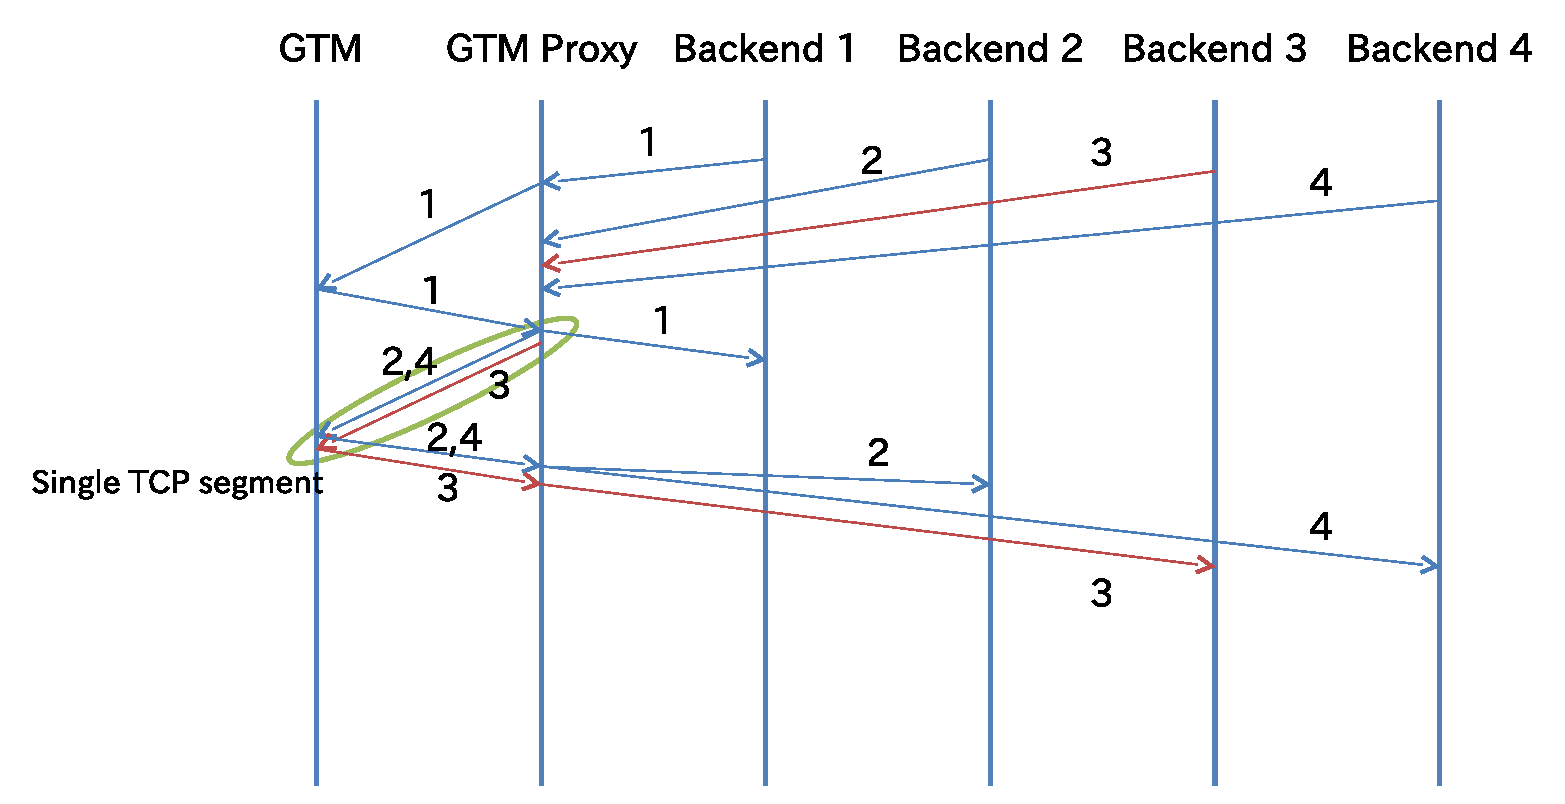
\includegraphics[width=0.9\hsize]{txn_gtmpxy.eps}
		  \caption{\label{fig:txngtmpxy}Example of GTM Proxy}
	  \end{center}
  \end{figure}
  
  These characteristics are brought from the internal structure of the GTM proxy.
  
  The GTM proxy is implemented with the worker thread model, and single thread handles multiple
  connections from the backends and single connection to GTM.
  After the main server loop \file{src/gtm/proxy/proxy_main.c:ServerLoop()} accepts a connection
  from a backend, the connection is dispatched to worker process in
  \file{proxy_main.c:GTMProxyAddConnection()}.
  The example used one worker thread.
  
  \file{proxy_main.c:GTMProxy_ThreadMain()} is the main loop of worker threads.
  This loop has two phases.

  1st phase reads data from all backend connections, and call \file{ProcessCommand()} to dispatch
  received message to \texttt{Process\textit{XXXXXXXX}Command()}.
  If the message is packable, \texttt{Processi\textit{XXXXXXXX}Command()} calls
  \file{GTMProxy_CommandPending()} to store the information.
  If the message is not packaged, {\tt } calls \file{GTMProxy_ProxyCommand()} to propagate the
  message immediately to GTM.
  Please note that the response is not received here.
  When all connections has no pending data, received messages are packed into single message,
  which is send it to the GTM.
  
  2nd phase reads data from the GTM connection and call \file{ProcessResponse()} to distribute
  received response to the backends.
  2nd phase is repeated until all response correspond to the message received in 1st phase.
  
  Because GTM proxy groups more than one message from coordinator/datanode backend into single
  packed message, it needs dedicated error handling.
  GTM protocol was extended to handle this.
  Without GTM proxy, GTM had direct connection to the backend.
  So the GTM automatically aborted transaction to cleanup transactions implicitly aborted when
  the connection is disconnected.
  With the GTM proxy, the GTM proxy holds connection even if one of the backend's connection
  handled by a thread disconnected.
  To avoid the transaction is left, the some packed message includes connection ID that identify
  the connection received the message.
  And the GTM proxy sends \file{MSG_BACKEND_DISCONNECT} to notify a disconnection of a backend.
  Please note that \file{MSG_BACKEND_DISCONNECT} message's body doesn't have connection ID.
  The message notifies the connection ID using \file{ProxyHdr} which is inserted to every message's
  body by the GTM proxy.



%%%%%%%%%%%%%%%%%%%%%%%%%%%%%%%%%%%%%%%%%%%%%%%%%%%%%%%%%%%%%%%%%%%%%%%%%%%%%%%%
%
% Backend Transaction Management
%
%%%%%%%%%%%%%%%%%%%%%%%%%%%%%%%%%%%%%%%%%%%%%%%%%%%%%%%%%%%%%%%%%%%%%%%%%%%%%%%%

%========= SECTION SECTION ===================================================

\section{Transaction Management at coordinator/datanode backends}

  Each coordinator/datanode backend needs to connect to GTM to obtain Global Transaction
  Id (\texttt{GXID}) and global snapshot.
  \file{gtm.c} module in \file{src/backend/access/transam} takes care of connection and
  communication between each backend and GTM.
  
  This section describes functions defined in \file{gtm.c} and other dedicated transaction
  handling related to GTM in coordinator/datanode backend processes.
  

%------- Subsec Subsec -----------------------------------------------------

\subsection{\texttt{gtm.c} module}
  
  \file{gtm.c} module handles connection and communication from coordinator/datanode
  backend and gtm/gtm\_proxy.
  
  Functions defined in this module are as follows:
  
  \FUNC{IsGTMConnected()}
  
      This function checks if connection to GTM is alive.
	  This is called from the following code:
      
	  % Function cross reference
      \FuncRefHdr
		  \FuncRef{AtEOXact_GlobalTxn()}{xact.c}{
			Used to determine what transaction ID should be used at the end of the
			transaction.
		  }\\ \hline
      \FuncRefTrailor
  
  
  \FUNC{CheckConnection()}
  
      This function checks if a connection to GTM has been established.
	  If not, it establishes a connection to GTM.
      
      This is a static function and is used only in \file{gtm.c} locally.
  
  \FUNC{InitGTM()}
  
      This function establishes a connection to GTM 
      and is used only within \file{gtm.c} at present.
  
  \FUNC{CloseGTM()}
  
      This function closes a connection to GTM
	  This is called from the following code:
      
	  % Function cross reference
      \FuncRefHdr
		  \FuncRef{PGXCNodeCleanAndRelease()}{execRemote.c}{
			Called when the backend is ending.
		  }\\ \hline
      \FuncRefTrailor
      
      This function is also called within \file{gtm.c} module internally.
  
  \FUNC{BeginTranGTM()}
  
      This function informs GTM of the start of a new transaction and obtains
      global transaction ID (\texttt{GXID}).
      
      This function is called from the following codes:
      
	  % Function cross reference
      \FuncRefHdr
		  \FuncRef{GetNewTransactionId()}{varsup.c}{
			Called to obtain global transaction ID.
		  }\\
		  \FuncRef{GetAuxilliaryTransactionId()}{xact.c}{
			Used to set auxilliaryTransactionId entry to CurrentTransactionState.
		  }\\ \hline
      \FuncRefTrailor
  
  \FUNC{BeginTranAutovacuumGTM()}
  
      This function is similar to \file{BeginTranGTM()} but only for autovacuum process.
      GXID for autovacuum process does not appear in the global snapshot.
      
      This function is called from the following codes:
      
      \FuncRefHdr
		  \FuncRef{GetNewTransactionId()}{varsup.c}{
			Called when obtaining XID for autovacuum process.
		  }\\ \hline
      \FuncRefTrailor
  
  \FUNC{CommitTranGTM()}
  
      This function tells GTM the specified transaction is committed and sets
      current transaction ID to invalid value.
      
      This is called from the following codes:
      
	  % Function cross reference
      \FuncRefHdr
		  \FuncRef{AtEOXact\_GlobalTxn()}{xact.c}{
			Called at the end of global transaction.
			It is called only when it is needed to close the transaction on the GTM
		  }\\ \hline
      \FuncRefTrailor
  
  \FUNC{CommitPreparedTranGTM()}
  
      This function tells GTM to commit a prepared transaction.
      
      This is called from the following codes:
      
	  % Function cross reference
      \FuncRefHdr
		  \FuncRef{AtEOXact_GlobalTxn()}{xact.c}{
			Used to mark the end of global transaction.
		  }\\
		  \FuncRef{FinishRemotePreparedTransaction()}{execRemote.c}{
			Used to finish prepared transaction at remote nodes.
		  }\\ \hline
      \FuncRefTrailor
  
  \FUNC{RollbackTranGTM()}
  
      This function tells GTM the specified transaction is aborted and
      sets current transaction ID to invalid value.
      
      This is called from the following codes:
      
	  % Function cross reference
      \FuncRefHdr
		  \FuncRef{AtEOXact_GlobalTxn()}{xact.c}{
			Called to mark the end of global transaction.
		  }\\
		  \FuncRef{FinishRemotePreparedTransaction()}{execRemote.c}{
			Called to finish prepared transaction at remote nodes.
		  }\\ \hline
      \FuncRefTrailor
  
  \FUNC{StartPreparedTranGTM()}
  
      This function tells GTM that prepare transaction commands starts with remote nodes.
      
      This is called from the following codes:
      
      \FuncRefHdr
		  \FuncRef{PreAbort_Remote()}{execRemote.c}{
			Called to abort remote truncations.
		  }\\
		  \FuncRef{PostPrepare_Remote()}{execRemote.c}{
			Called in post-prepare handling in remote nodes.
		  }\\ \hline
      \FuncRefTrailor
  
  \FUNC{PrepareTranGTM()}
  
      This function tells GTM that prepare transaction commands was successful.
      
      This is called from the following codes:
      
	  % Function cross reference
      \FuncRefHdr
		  \FuncRef{PreAbort_Remote()}{execRemote.c}{
			Called at re-abort handling.
		  }\\
		  \FuncRef{PostPrepare_Remote()}{execRemte.c}{
			Called at post-prepare handling.
		  }\\ \hline
      \FuncRefTrailor
  
  \FUNC{GetGIDDataGTM()}
  
      This function obtains GTM internal information of fresh GXID, GXID of the prepared
	  transaction, and datanode/coordinator node list involved in the prepare.
      
      This is for the future use.
  
  \FUNC{GetSnapshotGTM()}
  
      This function obtains global snapshot from GTM.
      
      This is called from the following codes:
      
	  % Function cross reference
      \FuncRefHdr
		  \FuncRef{GetSnapshotDataDataNode()}{procarray.c}{
			Called to get snapshot data for datanode.
		  }\\
		  \FuncRef{GetSnapshotDataCoordinator()}{procarray.c}{
			Called to get snapshot data for coordinator.
		  }\\ \hline
      \FuncRefTrailor
  
  \FUNC{CreateSequenceGTM()}
  
      This function creates a sequence on GTM.
      
      This is called from the following codes:
      
	  % Function cross reference
      \FuncRefHdr
		  \FuncRef{DefineSequence()}{sequence.c}{
			Called in creating sequence.
		  }\\ \hline
      \FuncRefTrailor
  
  \FUNC{AlterSequenceGTM()}
  
      This function alters a sequence on GTM.
      
      This is called from the following code:
      
	  % Function cross reference
      \FuncRefHdr
		  \FuncRef{AlterSequence()}{sequence.c}{
			Called to modify the definition of a sequence.
		  }\\ \hline
      \FuncRefTrailor
  
  \FUNC{GetNextValGTM()}
  
      This function gets the next sequence value.
      
      This is called from the following codes:
      
	  % Function cross reference
      \FuncRefHdr
      \FuncRef{nextval\_internal()}{sequence.c}{
      	Called to get the next value of the sequence.
      }\\ \hline
      \FuncRefTrailor
  
  \FUNC{SetValGTM()}
  
      This functions sets the value of the sequence.
      
      This is called form the following codes:
      
	  % Function cross reference
      \FuncRefHdr
		  \FuncRef{do_setval()}{sequence.c}{
		  This is called in handling 2 and 3 argument forms of {\tt SETVAL}.
		  }\\ \hline
      \FuncRefTrailor
  
  \FUNC{DropSequenceGTM()}
  
      This function drops sequence depending on the key type.
      
      This is called from the following codes:
      
	  % Function cross reference
      \FuncRefHdr
		  \FuncRef{drop_sequence_cb()}{sequence.c}{
			Called in a callback of sequence drop.
		  }\\
		  \FuncRef{dropdb()}{dbcommands.c}{
			Called in dropping a database.
		  }\\ \hline
      \FuncRefTrailor
  
  \FUNC{RenameSequenceGTM()}
  
      This function renames sequence on GTM.
      
      This is called from the following codes:
      
	  % Function cross reference
      \FuncRefHdr
		  \FuncRef{RenameRelationInternal()}{tablecmds.c}{
			Called in changing the name of a relation.
		  }\\
		  \FuncRef{AlterTableNamespaceInternal()}{tablecmds.c}{
			This is called in relocating a table or materialized view to another namespace.
		  }\\
		  \FuncRef{AlterSeqNamespaces()}{tablecmds.c}{
			This is called to move all {\tt SERIAL} column sequences of the specified relation
			to another namespace.
		  }\\
		  \FuncRef{rename_sequence_cb()}{sequence.c}{
			Called in sequence rename callback.
		  }\\
		  \FuncRef{doRename()}{dependency.c}{
			Called in renaming the given object.
		  }\\ \hline
      \FuncRefTrailor
  
  \FUNC{RegisterGTM()}
  
      This function registers the specified node to GTM.
      Connection for registering is used just once the closed.
      
      This is called from the following codes:
      
	  % Function cross reference
      \FuncRefHdr
		  \FuncRef{sigusr1_handler()}{postmaster.c}{
			Called in handling signal conditions from child processes.
		  }\\ \hline
      \FuncRefTrailor
  
  \FUNC{UnregisterGTM()}
  
      This function unregisters the given node from GTM.
      Connection for registering is used just once the closed.
      
      This is called form the following codes:
      
	  % Function cross reference
      \FuncRefHdr
		  \FuncRef{pmdie()}{postmaster.c}{
			Called in a signal handler to handle various postmaster signals.
		  }\\
		  \FuncRef{sigusr1_handler()}{postmaster.c}{
			Called in handling signal conditions from child processes.
		  }\\ \hline
      \FuncRefTrailor
  
  \FUNC{ReportBarrierGTM()}
  
      This function reports barrier to GTM.
      This is used to backup GTM restart point for given barrier id.
      
	  % Function cross reference
      \FuncRefHdr
		  \FuncRef{RequestBarrier()}{barrier.c}{
			Called in handling \texttt{CREATE BARRIER} statement.
		  }\\ \hline
      \FuncRefTrailor


%------- Subsec Subsec -----------------------------------------------------

\subsection{\texttt{xact.c} module}

  This module has \XC-specific functions as follows:
  
  \FUNC{RegisterTransactionLocalNode()}
  
      Marks if the local node has done some write activity.
      
      This is called form the following codes:
      
	  % Function cross reference
      \FuncRefHdr
		  \FuncRef{ExecRemoteUtility()}{execRemote.c}{}\vspace{-10pt} \\ \hline
      \FuncRefTrailor
  
  \FUNC{ForgetTransactionLocalNode()}
  
      Forgets about the local node's involvement in the transaction.
      
      Called from the following codes:
      
	  % Function cross reference
      \FuncRefHdr
		  \FuncRef{CommitTransaction()}{xact.c}{}\vspace{-10pt} \\
		  \FuncRef{PrepareTransaction()}{xact.c}{}\vspace{-10pt} \\
		  \FuncRef{AbortTransaction()}{xact.c}{}\vspace{-10pt} \\ \hline
      \FuncRefTrailor
  
  \FUNC{IsTransactionLocalNode()}
  
      Checks if the local node is involved in the transaction.
      
      Called form the following codes:
      
      It is for the future use and is not used at present.
  
  \FUNC{IsXidImplicit()}
  
      Checks if the given xid is for implicit 2PC.
      
      Called form the following code:
      
	  % Function cross reference
      \FuncRefHdr
		  \FuncRef{standard_ProcessUtility()}{utility.c}{
			Called in handling \texttt{PREPARE TRANSACTION} command.
		  }\\ \hline
      \FuncRefTrailor
	% Koichi


%%%%%%%%% CHAPTER CHAPTER CHAPTER %%%%%%%%%%%%%%%%%%%%%%%%%%%%%%%%%%%%%%%%%%%%%%%%%%

\chapter{\label{chap:plannerExecutor}Planner and Executor}

%%%%%%%%%%%%%%%%%%%%%%%%%%%%%%%%%%%%%%%%%%%%%%%%%%%%%%%%%%%%%%%%%%%%%%%%%%%%%%%%
%
% Planner and Executor
%
%%%%%%%%%%%%%%%%%%%%%%%%%%%%%%%%%%%%%%%%%%%%%%%%%%%%%%%%%%%%%%%%%%%%%%%%%%%%%%%%

  This chapter describes implementaion of \texttt{SELECT} statement and other DML handling.
  
  As described in section~\ref{pgxc:FQS} at page~\pageref{pgxc:FQS}, \file{planner()}
  in \file{planner.c} is the entry point of all the \PG~ and \XC's planner.
  
  In vanilla \PG, if no planner hook is defined, it is handled by \file{standard_planner()}.
  In \XC, in the originating coordinator, it is handled by \file{pgxc_planner()} instead.
  In the case of datanode or non-originating coordinator where
  the statement is shipped from other coordinator,
  it is handled by \file{standard_planner()} just like vanilla \PG.
  
  \file{pgxc_planner()} is implemented in \file{pgxcplan.c}, where the statement is handled by
  \file{pgxc_handle_unsupported_stmts()} to check if given statements are not supported by \XC.
  If a statement is not supported, then it is treated as an error and the planner returns.
  If all the statements are suported ones, it is passed to \file{pgxc_FQS_planner()} to check if
  the whole statement can be shipped to one or more nodes.
  If so, then the planner returns the plan to the caller.
  If not, then the statement is passed to \file{standard_planner()} for further work.
  
  \file{pgxcplan.c} implements many utility functions used in the planner, as described in
  section~\ref{pgxc:FQS} in page~\pageref{pgxc:FQS}.
  
  There's no \XC-specific code in \file{standard_planner()} and all \XC-specific
  functionarities are 
  implemented in other functions called from here.
  
  Another module to produce remote plan is \file{pgxcpath.c}, which creates all the
  remote execute plan
  as the node \file{RemoteQueryPath} defined in \file{relation.h}.
  Functions defined in this module is described in the section~\ref{additional:pgxcpath} at
  page \pageref{additional:pgxcpath}.


%========= SECTION SECTION ===================================================

\section{\label{sec:joinPushdown}Join Pushdown}

  Join pushdown is handled in the funciton \file{create_joinrel_rqpath()} as described in
  subsection~\ref{additional:pgxcpath} on page \pageref{additional:pgxcpath}.
  
  This function assumes at least one of the join relations has remote query path
  and checks the path to outer relation and innter relation.
  Each path has already been set up by \file{create_plainrel_rqpath()} function defined in
  \file{pgxcpath.c}.
  If either relation does not have remote path, then this function returns without changing
  the original plan.
  In this case, typically join with system catalog or materialized view, remote relation is
  materialized at the coordinator and subsequent join operation is performed locally at
  the coordinator.
  
  Then it checks if outer join is path is still parameterized and it is not shippable.
  
  If shippable, it checks if join quals are shippable using \file{pgxc_is_expr_shippable()}
  defined in \file{pgxcship.c}.
  In fact, shippability of each qual has already been set up by \file{create_remotequery_path()}
  defined in \file{pgxcpath.c}.
  
  Next, if join is innter join, all the other quals are combined with join quals to be pushed down.
  Quals other than join quals are not pushed down in the case of outer join.
  This can be improved in the future.
  
  Now, all the join fell into simple structure and is ready to check whole join shippability and
  to build the plan into \file{ExecNodes} structure by \file{pgxc_is_join_shippable()} defined in
  \file{pgxcship.c}.
  
  Here, shippability condition is as follows:
  
  \begin{itemize}
	  \item Both outer and innter relation has \file{ExecNodes}.
	  \item Join type is inner join, left outer join or full join.   Right outer join is not pushed down.
	  \item In the case of left outer join, inner relation path must be shippable.
	  \item In the case of full outer join, both innter and outer relation path must be shippable.
	  \item Both inner and outer relation are replicated table.
	  \item If both inner and outer relation are distributed, then two of them should be
	  		distributed in the same manner, with equi-join on the distribution column and
			the condition is shippable.
			In this case, the result is merged at the coordinator.
	  \item If outer relation is distributed and inner one is replicated, both left outer join and
	  		inner join are pushed down.
	  \item If outer relation is replicated and inner one is distributed, only inner join is pushed down.
	  \item \file{ExecNodes} of inner and outer nodes should be able to be merged.
  \end{itemize}
  
  Again, if \file{pgxc_is_join_shippable()} determines the join is not shippable, original path
  for inner and outer relations work to materialize them at coordinator and to do the rest of
  the join operations here in the originating coordinator.
  
  By this step, all the local quals have been pushed down to each path using \PG{} planner
  code to reduce the number of fetched rows.


%========= SECTION SECTION ===================================================

\section{\label{sec:orderBy}Order By Pushdown}

  \texttt{ORDER BY} pushdown is handled by \file{create_remotesort_plan():pgxcplan.c}.
  This function checks if \texttt{ORDER BY} (and any other sort function) can be pushed down
  and modifies pased in Sort plan and underlying \texttt{Remote Query} plan.


%========= SECTION SECTION ===================================================

\section{\label{sec:limit}Limit Pushdown}

  \texttt{LIMIt} pushdown is handled by \file{create_remotelimit_plan():pgxcplan.c}.
  Similar to \texttt{ORDER BY} push down, it checks if \texttt{LIMIT} clause is pushable.
  If so, then it pushes \file{limitcount} and \file{limitoffset} if defined.
  This is done by modifying \file{RemoteQuery} node.


%========= SECTION SECTION ===================================================

\section{\label{sec:groupBy}Group By Pushdown}

  \texttt{GROUP BY} pushdown is handled by \file{create_remotegrouping_plan():pgxcplan.c}.
  Current restriction is as follows:

  \begin{enumerate}
  	  \item Only plain aggregates (no expressions involving aggregates) and/or expressions in
	  		\texttt{GROUP BY} clause are pushed down.
	  \item \texttt{DISTINCT} and \texttt{ORDER BY} clause are not pushed down.
	  \item Window functions are not pushed down.
	  \item \texttt{HAVING} clause is not pushed down.
  \end{enumerate}

%========= SECTION SECTION ===================================================

\section{\label{sec:windowFunc}Window Function Handling}

  At present, window functions are not pushed down unless whole statement can be shipped.


%========= SECTION SECTION ===================================================

\section{\label{sec:aggregateFunc}Aggregate Function Handling}

  In \XC, aggregate function handling need an extension from \PG.
  The background is simple pushdown may not work for some kind of aggregate functions.
  For example, in the calculation of average, we cannot push down \file{avg()} function to
  datanodes to calculate global average.
  Instead, we need to obtain sum and count from each datanode to calculat the final result.

  For this extension, \XC{} introduced new function layer called \textbf{collector function}.
  The document is available at
  \url{http://postgres-xc.sourceforge.net/docs/1_2_1/sql-createaggregate.html}.

  Internally, for example, \file{avg()} function definition in the system catalog is
  defined in \file{pg_aggregate.h} as shown in
  \url{http://postgres-xc.sourceforge.net/docs/1_2_1/catalog-pg-aggregate.html}.

  In \file{pg_aggregate} system catalog, column \file{aggcollectfn} was added to define
  new collector function.
  Definition of \file{avg()} function in \file{pg_aggregate.h} source code is as follows:

  % Source listing ---------------------------------------
  \begin{lstlisting}[tabsize=4, frame=single]
/* avg */
#ifdef PGXC
  DATA(insert ( 2100  int8_avg_accum  numeric_avg_collect numeric_avg     0   1231    "{0,0}" "{0,0}" ));
  DATA(insert ( 2101  int4_avg_accum  int8_avg_collect    int8_avg        0   1016    "{0,0}" "{0,0}" ));
  DATA(insert ( 2102  int2_avg_accum  int8_avg_collect    int8_avg        0   1016    "{0,0}" "{0,0}" ));
  DATA(insert ( 2103  numeric_avg_accum   numeric_avg_collect numeric_avg     0   1231    "{0,0}" "{0,0}" ));
  DATA(insert ( 2104  float4_accum    float8_collect  float8_avg      0   1022    "{0,0,0}" "{0,0,0}" ));
  DATA(insert ( 2105  float8_accum    float8_collect  float8_avg      0   1022    "{0,0,0}" "{0,0,0}" ));
  DATA(insert ( 2106  interval_accum  interval_collect    interval_avg    0   1187    "{0 second,0 second}" "{0 second,0 second}" ));
#endif
  \end{lstlisting}
  % End source listing -----------------------------------

  In each line with \file{DATA} keyword, the second function corresponds to the collector function for various data types.

  Example of collector function is as follows:

  % Source listing ---------------------------------------
  \begin{lstlisting}[tabsize=4, frame=single]
Datum
int8_avg_collect(PG_FUNCTION_ARGS)
{
	ArrayType  *collectarray;
	ArrayType  *transarray = PG_GETARG_ARRAYTYPE_P(1);
	Int8TransTypeData *collectdata;
	Int8TransTypeData *transdata;

	/*
	 * If we're invoked by nodeAgg, we can cheat and modify our first
	 * parameter in-place to reduce palloc overhead. Otherwise we need to make
	 * a copy of it before scribbling on it.
	 */
	if (fcinfo->context &&
		(IsA(fcinfo->context, AggState) ||
		 IsA(fcinfo->context, WindowAggState)))
		collectarray = PG_GETARG_ARRAYTYPE_P(0);
	else
		collectarray = PG_GETARG_ARRAYTYPE_P_COPY(0);

	if (ARR_HASNULL(collectarray) ||
	    ARR_SIZE(collectarray) != ARR_OVERHEAD_NONULLS(1) + sizeof(Int8TransTypeData))
		elog(ERROR, "expected 2-element int8 array");
	collectdata = (Int8TransTypeData *) ARR_DATA_PTR(collectarray);

	if (ARR_HASNULL(transarray) ||
	    ARR_SIZE(transarray) != ARR_OVERHEAD_NONULLS(1) + sizeof(Int8TransTypeData))
		elog(ERROR, "expected 2-element int8 array");
	transdata = (Int8TransTypeData *) ARR_DATA_PTR(transarray);

	collectdata->count += transdata->count;
	collectdata->sum += transdata->sum;

	PG_RETURN_ARRAYTYPE_P(collectarray);
}
  \end{lstlisting}
  % End source listing -----------------------------------

\section{\label{sec:seqExec}Global Sequence Implementation}

  \XC{} has to ensure the uniqueness of the sequence value in a cluster.
  Similar to global transaction management, coordinators needs sequence management
  of global tables on GTM.
  GTM is responsible for it.
  GTM-side implementaion is described in section \ref{sec:gtm} at page~\pageref{sec:gtm}.

  The global tables mentioned above doesn't include temporary tables.
  \XC{} manages the sequences on temporary tables locally just
   like \PG{} does.

  \XC{} didn't modify sequence handling in core planner and the executor.

  Major changes in sequence handling are listed below:

  \begin{itemize}
  	\item Define a new sequence:
		\begin{enumerate}
			\item Define a new sequence
			\item Call \file{CreateSequenceGTM()} to register sequence information to GTM.
            \item Define a local relation for the new sequence.
            \item Register a callback function to drop the defined sequence when the transaction is aborted. 
		\end{enumerate}
	\item Alter sequence information
		\begin{enumerate}
			\item Call \file{AlterSequenceGTM()} to alter sequence information in GTM.
            \item Update local sequence information.
		\end{enumerate}
	\item Rename a sequence
		\begin{enumerate}
			\item Call \file{RenameSequenceGTM()} to rename the sequence in GTM.
            \item Update local sequence information.
            \item Register a callback function to rename the renamed sequence to original name when the transaction is aborted. 
		\end{enumerate}
	\item Get next sequence values
		\begin{enumerate}
			\item Call \file{GetNextValGTM()} to rename the sequence in GTM.
            \item Update local sequence information with the values returned by GTM.
		\end{enumerate}
	\item Set sequence value
		\begin{enumerate}
			\item Call \file{SetValGTM()} to set the sequence value in GTM. 
            \item Update local sequence information. 
		\end{enumerate}
  \end{itemize}
		
  Did you find that the coordinators have sequence relations like \PG?
  Yes, you can refer cached value at there.
  But please note that the sequence values in GTM could be modified by other coordinators.
  So \file{pg_dump} calls \file{nextval} SQL function to obtaion latest value
   instead of looking the sequence tables.




%%%%%%%%% CHAPTER CHAPTER CHAPTER %%%%%%%%%%%%%%%%%%%%%%%%%%%%%%%%%%%%%%%%%%%%%%%%%%

\chapter{\label{chap:DML}DML}

%
% This file includes design and implementation of DML handling in Postgres-XC.
%


%========= SECTION SECTION ===================================================

\section{\label{sec:insert}Top level statment}

  Basically, XC does not handle {\tt INSERT}, {\tt UPDATE} and {\tt DELETE}
  statements specifically except for replicated table handling.
  
  These statements are analyzed, rewritten and planned before execution.
  Subqueries are also planned using vanilla \PG{} code.
  During the analyze, remote tables are marked and they are planned into {\tt RemoteQuery}.


%========= SECTION SECTION ===================================================

\section{\label{sec:returning}Returning Clause}

  If any statement has {\tt RETURNING} clause, this information is set to {\tt retruningList}
  member of {\tt Query} structure.
  If DML has {\tt RETURNING} clause, this information is set to {\tt returningList} member of
  {\tt InsertStmt}, {\tt DeleteStmt} and {\tt UpdateStmt} structure.
  It is vanilla \PG~structure and no modification was made in \XC.
  
  So far, {\tt RETURNING} clause is handled as shippable in \XC, as found in
  {\tt pgxc\_shippability\_walker()}.


%========= SECTION SECTION ===================================================

\section{\label{sec:repTableDML}DML Handling for Replicated Tables}

  In updating repliated tables, 
  each coordinator visits \textbf{bf primary} node first gor each replicated table updates.
  This is needed to serialize conflicting updates and to prevent inconsisitent updates among nodes.
  By doing this, when updates at primariy node is successful, then coordinator can visit
  other nodes in any order.
  Conflicting transactions will be blocked at primary node until the first successful transaction
  finishes.

  Through analyzer and other functions, primary node list of a given replicate table will be
  set to the member \file{primarynodelist}  of \file{ExecNodes} structure by
  \file{GetRelationNodes():locator.c}.
  This value is tested in the executor, \file{executeRemote.c}.
  In the case of copy in (copying tuples to a table), it is handled by \file{DataNodeCopyIn():execRemote.c}.
  If primary node is defined for the rlation, the executor extracts one connection to a primary node and
  handle this first before other replica are handled.

  Similar handling was done in \file{get_exec_connections():execRemote.c} and
  \file{redustrub.c:distrib_copy_from()} too.



%========= SECTION SECTION ===================================================

\section{\label{sec:copy}Copy statement handling}

  \texttt{COPY TO} collects data from datanodes and \texttt{COPY FROM} distributes data to datanodes.
  These are quite similar to \texttt{INSERT} and \texttt{SELECT} and look like a DML.
  But actually they are utility statements.
  In addition to distinct implementation,
  \texttt{COPY} statements have to calcurate which node and what query to send by themselevs
  because the planner doesn't analyze utility statements
  and doesn't locate where to go the query for them.
  There's a point here. When the coordinator received \texttt{COPY FROM},
  the query doesn't specify column with non-shippable default value,
  the coordinator have to complete both a query and data.
  
  In addition, \texttt{COPY} processes data in consecutive segments.
  It means the following actions will be taken in parallel.
  
  \begin{itemize}
    \item Coordinator receives data from client and propages it to datanodes
    \item Datanodes receive data from a coordinator and processes it
  \end{itemize}
  
  To calculate involved nodes and save distribution information into \file{struct RemoteCopyState},
   \file{RemoteCopy_GetRelationLoc()} is implemented.
  And \file{RemoteCopy_BuildStatement()} builds the query shipped to datanodes.
  Ofcourse the built query includes the column which has non-shippable default value.
  These functions are called from \file{BeginCopy()}.
  This function is common to \texttt{COPY TO} and \texttt{COPY FROM}.
  
  \file{CopyFrom()} processes \texttt{COPY FROM} statement.
  To begin the copy, \file{pgxcNodeCopyBegin()} prepares a global transaction and connections to
  datanodes and send \texttt{COPY FROM} query to datanodes.
  Each copied data obtained from \PG{} client by \file{NextCopyFrom()} is checked which node
  to go by \file{GetRelationNodes()} and it is sent to datanodes by \file{DataNodeCopyIn()}.
  If \file{COPY FROM} need to support binary format data, the signature that indicates binary
  mode need to be sent to datanodes just after the query is sent to datanodes.
  
  \file{CopyTo()} processes \texttt{COPY TO} statement.
  To begin the copy, \file{pgxcNodeCopyBegin()} prepares a global transaction and connections to
  datanodes and send \texttt{COPY TO} query to datanodes.
  \file{DataNodeCopyOut()} reads copied data from each connection to datanode until it receives
  message with type '\texttt{Z}' (Ready For Query) in \file{handle_response()}.
  Copied data rows will come as messages with type '\texttt{d}' (CopyOutDataRow).
  They are handled in \file{HandleCopyDataRow()} using the storage specified at the combiner.
  If \texttt{COPY TO} need to support binary format data, the signature that indicates binary mode
  need to be sent to \PG{} client just after the query is sent to datanodes.
  
  \texttt{COPY} statement is implemented in \file{src/backend/command/copy.c} and main part of
  \XC{} specific logic is in \file{src/backend/pgxc/copy/remotecopy.c} and
  \file{src/backend/pgxc/pool/execRemote.c}.
  \file{remotecopy.c} has utility functions used in \file{copy.c}.
  For example, \file{RemoteCopy_GetRelationLoc()} creates \file{RelationLocInfo}
  which has location information of relations involved to the query.
  \file{RemoteCopy_BuildStatement()} builds a copy query executed at datanodes.
  \file{execRemote.c} has functions to execute actual process of the copy command
  using information prepared in \file{copy.c}.
  Examples include \file{pgxcNodeCopyBegin()} and \file{DataNodeCopyIn()}.
  




%%%%%%%%% CHAPTER CHAPTER CHAPTER %%%%%%%%%%%%%%%%%%%%%%%%%%%%%%%%%%%%%%%%%%%%%%%%%%

\chapter{\label{chap:func}Session and system functions}

%%%%%%%%%%%%%%%%%%%%%%%%%%%%%%%%%%%%%%%%%%%%%%%%%%%%%%%%%%%%%%%%%%%%%%%%%%%%%%%%
%
% XC-specific function description
%
%%%%%%%%%%%%%%%%%%%%%%%%%%%%%%%%%%%%%%%%%%%%%%%%%%%%%%%%%%%%%%%%%%%%%%%%%%%%%%%%
  This chapter describes additional session and system functions for \XC.
  
  \FUNC{xc_pool_reload()}
  
      This function refreshes cached information of \file{pgxc_node} catalog and cleans up
	  pooled connections managed by the pooler.
  
  \FUNC{is_committed(transaction_id)}
  
      This function reoprts if a transaction with given GXID is committed or not.
      Returned information is just local to the issued node.
      This is intended to be used in \file{pgxc_clean} or other utilities to cleanup and
	  recover commit status of any two-phase commit transactions.
  
  \FUNC{pgxc_version()}
  
      This function returns \XC~ version.
  
  \FUNC{pgxc_pool_check()}
  
      This function checks if connection data cached in the pooler is consistent
	  with \file{pgxc_node}.
  
  \FUNC{pgxc_lock_for_backup()}
  
      This function locks the cluster for taking backup of the node to be exported to the new
	  node being added.



%%%%%%%%% CHAPTER CHAPTER CHAPTER %%%%%%%%%%%%%%%%%%%%%%%%%%%%%%%%%%%%%%%%%%%%%%%%%%

\chapter{\label{chap:misc}Miscellaneous Feature}

%%%%%%%%%%%%%%%%%%%%%%%%%%%%%%%%%%%%%%%%%%%%%%%%%%%%%%%%%%%%%%%%%%%%%%%%%%%%%%%%
%
% Miscellaneous Feature section.   Describes additional GUCS to Postgres-XC.
%
%%%%%%%%%%%%%%%%%%%%%%%%%%%%%%%%%%%%%%%%%%%%%%%%%%%%%%%%%%%%%%%%%%%%%%%%%%%%%%%%


%========= SECTION SECTION ===================================================

\section{\label{sec:GUC}Additional \texttt{postgresql.conf} configuration parameters}

  This section describes additional \file{postgresql.conf} configuration parameters specific to \XC.


%------- Subsec Subsec -----------------------------------------------------

\subsection*{\label{subsec:enableFQS}\texttt{enable\_fast\_query\_shipping}}

  This is boolean parameter to specify if fast query shipping is enabled.
  Usually this should be {\tt ON}.


%------- Subsec Subsec -----------------------------------------------------

\subsection*{\label{subsec:enableRemotegroup}\texttt{enable\_remotegroup}}

  This is boolean parameter to specify if group-by push down to remote nodes is enabled.
  Usually this should be {\tt ON}.


%------- Subsec Subsec -----------------------------------------------------

\subsection*{\label{subsec:enableRemotejoin}\texttt{enable\_remotejoin}}

  This is boolean parameter to specify if join push down to remote nodes is enabled.
  Usually this should be {\tt ON}.


%------- Subsec Subsec -----------------------------------------------------

\subsection*{\label{subsec:enableRemotelimit}\texttt{enable\_remotelimit}}

  This is boolean parameter to specify if limit pushdown to remote nodes is enabled.
  Usually this should be {\tt ON}.


%------- Subsec Subsec -----------------------------------------------------

\subsection*{\label{subsec:enableRemotesort}\texttt{enable\_remotesort}}

  This is boolean parameter to specify if ORDER BY pushdown to remote node is enabled.
  Usually this should be {\tt ON}.


%------- Subsec Subsec -----------------------------------------------------

\subsection*{\label{subsec:enforceTwoPhaseCommit}\texttt{enforce\_two\_phase\_commit}}

  This is boolean parameter to specify if two phase commit protocol is used for
  write transactions more than two nodes are involved.


%------- Subsec Subsec -----------------------------------------------------

\subsection*{\label{subsec:gtmBackupBarrier}\texttt{gtm\_backup\_barrier}}

  This is boolean parameter to specify if GTM restart point is backed up for barrier.


%------- Subsec Subsec -----------------------------------------------------

\subsection*{\label{subsec:gtmHost}\texttt{gtm\_host}}

  This is character string parameter to specify host name of GTM.
  If you configure GTM proxy, you should specify host name of GTM proxy.


%------- Subsec Subsec -----------------------------------------------------

\subsection*{\label{subsec:gtmPort}\texttt{gtm\_port}}

  This is integer parameter to specify port number of GTM.
  If you configure GTM proxy, you should specify port number of GTM proxy.


%------- Subsec Subsec -----------------------------------------------------

\subsection*{\label{subsec:maxCoordinators}\texttt{max\_coordinators}}

  This is integer parameter to specify the maximum number of coordinators in the cluster.


%------- Subsec Subsec -----------------------------------------------------

\subsection*{\label{subsec:maxDatanodes}\texttt{max\_datanodes}}

  This is numeric parameter to specify the maximum number of datanodes in the cluster.


%------- Subsec Subsec -----------------------------------------------------

\subsection*{\label{subsec:maxPoolSize}\texttt{max\_pool\_size}}

  This is numeric parameter to specify the maximum number of pooled connection in the pooler.


%------- Subsec Subsec -----------------------------------------------------

\subsection*{\label{subsec:minPoolSize}\texttt{min\_pool\_size}}

  This is numeric parameter to specify the minimum number of pooled connection in the pooler.


%------- Subsec Subsec -----------------------------------------------------

\subsection*{\label{subsec:persistentDatanodeConnections}\texttt{persistent\_datanode\_connections}}

  This is boolean parameter to specify if the connections from coordinator to datanodes should keep assigned.


%------- Subsec Subsec -----------------------------------------------------

\subsection*{\label{subsec:pgxcNodename}\texttt{pgxc\_node\_name}}

  This is character string parameter to specify the node name of itself.

\subsection*{\label{subsec:poolerPort}\texttt{pooler\_port}}

This is numeric parameter to specify the port number of the pooler.


%------- Subsec Subsec -----------------------------------------------------

\subsection*{\label{subsec:remoteType}\texttt{remotetype}}

  Used to identify what is connecting to the backend.
  Usually, do not modify this parameter.


%------- Subsec Subsec -----------------------------------------------------

\subsection*{\label{subsec:requireRepTablePkey}\texttt{require\_replicated\_table\_pkey}}

  Boolean parameter to specify if it is not allowed replicated tables without primary key or another unique key combination involved.
  If this is turned on and no such unique key is not involved, the statement fails.


%------- Subsec Subsec -----------------------------------------------------

\subsection*{\label{subsec:maintenanceMode}\texttt{xc\_maintenance\_mode}}

  Boolean parameter to control if write operation is allowed in {\tt EXECUTE DIRECT}.
  This parameter cannot turn on in {\tt postgresql.conf}.
  Only a superuser can turn it on in a session.


%------- Subsec Subsec -----------------------------------------------------

\section{\label{sec:syntax}Additional SQL syntax for \XC}

  The following lists \XC-specific SQL statement syntax.
  Refer to \XC~ documentation for details.
  
  \begin{itemize}
	  \item \texttt{ALTER NODE} statement.
	  \item \texttt{DISTRIBUTE BY} clause in \texttt{ALTER TABLE} statement.
	  \item\texttt{CLEAN CONNECTION} statement.
	  \item Collection function in \texttt{CREATE AGGREGATE} statement.
	  \item \texttt{CREATE BARRIER} statement.
	  \item \texttt{CREATE NODE} statement.
	  \item \texttt{CREATE NODE GROUP} statement.
	  \item Additional options for \texttt{EXPLAIN} statement.
	  \item \texttt{DISTRIBUTE BY} clause in \texttt{CREATE TABLE} statement.
	  \item \texttt{DROP NODE} statement.
	  \item \texttt{DROP NODE GROUP} statement.
  \end{itemize}



%%%%%%%%% CHAPTER CHAPTER CHAPTER %%%%%%%%%%%%%%%%%%%%%%%%%%%%%%%%%%%%%%%%%%%%%%%%%%

\chapter{\label{chap:regression}Regression Tests}

%%%%%%%%%%%%%%%%%%%%%%%%%%%%%%%%%%%%%%%%%%%%%%%%%%%%%%%%%%%%%%%%%%%%%%%%%%%%%%%%
%
% Chapter "Regression".
%
% Description of additional regression test for Postgres-XC.
%
%%%%%%%%%%%%%%%%%%%%%%%%%%%%%%%%%%%%%%%%%%%%%%%%%%%%%%%%%%%%%%%%%%%%%%%%%%%%%%%%


  This chapter describes changes to regression test.


%========= SECTION SECTION ===================================================

\section{General Changes}

  Most of the statements in the regression tests are used as is, or with minimum modification.
  General modification for \XC{} is as follows:
  
  \begin{itemize}
	  \item No \texttt{DISTRIBUTE BY} clause was given to \texttt{CREATE TABLE} or \texttt{ALTER TABLE}
	  		statement, if the first column is allowd as the distribution column.
	  \item If the first column is not allowd as the distribution column and another column
	  		is found suitable, \texttt{DISTRIBUTE BY HASH(}\textit{colname}\texttt{)}
			clause is added.
	  \item If no column is suitable for the distribution column, such table was defined as
	  		replicated table using \texttt{DISTRIBUTE BY REPLICATION}.
	  \item Because order of rows of \texttt{SELECT} statement or \texttt{RETURNING} clause depends upon
	  		the order of execution among datanodes, \texttt{ORDER BY} clause was added to make this
			order reproductive.
	  \item To make \texttt{EXPLAIN} result portable, \texttt{NODES OFF} and
			\texttt{NUM\_NODES OFF} options were added to make test result independent from
			the number of nodes and their names.
  \end{itemize}
  
  For specific test purpose, some tables in existing \PG{} regression test are created as
  replicated or round-robin distribution.
  
  Example of additional use of \texttt{ORDER BY} clause in \file{join.sql} is shown below.

  % Source listing -----------------
  \lstset{tabsize=4, xleftmargin=20pt, basicstyle=\ttfamily\small, breaklines=true}
  \begin{lstlisting}[frame=single]
 184 -- Outer joins
 185 -- Note that OUTER is a noise word
 186 --
 187 
 188 SELECT '' AS "xxx", *
 189   FROM J1_TBL LEFT OUTER JOIN J2_TBL USING (i)
 190   ORDER BY i, k, t;
 191 
 192 SELECT '' AS "xxx", *
 193   FROM J1_TBL LEFT JOIN J2_TBL USING (i)
 194   ORDER BY i, k, t;
 195 
 196 SELECT '' AS "xxx", *
 197   FROM J1_TBL RIGHT OUTER JOIN J2_TBL USING (i)
 198   ORDER BY i, j, k, t;
  \end{lstlisting}

  Example of additional option use in \texttt{EXPLAIN} in \file{join.sql} is shown below.

  \lstset{tabsize=4, xleftmargin=20pt, basicstyle=\ttfamily\small, breaklines=true}
  \begin{lstlisting}[frame=single]
 705 --
 706 -- test case where a PlaceHolderVar is propagated into a subquery
 707 --
 708 
 709 explain (num_nodes off, nodes off, costs off)
 710 select * from
 711   int8_tbl t1 left join
 712   (select q1 as x, 42 as y from int8_tbl t2) ss
 713   on t1.q2 = ss.x
 714 where
 715   1 = (select 1 from int8_tbl t3 where ss.y is not null limit 1)
 716 order by 1,2;
 717 
 718 select * from
 719   int8_tbl t1 left join
 720   (select q1 as x, 42 as y from int8_tbl t2) ss
 721   on t1.q2 = ss.x
 722 where
 723   1 = (select 1 from int8_tbl t3 where ss.y is not null limit 1)
 724 order by 1,2;
  \end{lstlisting}
    
  Please note that \texttt{ORDER BY} clause is given only to the subsequent \texttt{SELECT} statement
  because regression test needs to test the plan without \texttt{ORDER BY} close while subsequent
  \texttt{SELECT} statement needs to produce portable result.

  Please also not that \texttt{COSTS OFF} option in \texttt{EXPLAIN} statements are from vanilla
  \PG{} regression test to make explain result portable too.


%========= SECTION SECTION ===================================================

\section{Additional Test for \XC}

  Regression test prefixed with \file{xc_} is \XC-specific regression test.
  
  Table~ \ref{tab:xcRegression} describes each test.
  
  \begin{table}[htp]
	  \begin{center}
	  \caption{\label{tab:xcRegression}\XC-specific Regression Test}
		  \begin{tabular}{lp{0.7\hsize}} \hline
			  Test Name & Description \\ \hline
			  \file{xc_alter_table} & Checks \XC-specific behavior of \texttt{ALTER TABLE} statement,
			  						   such as dropping distribution column is not allowed.\\
			  \file{xc_constraints} & Checks constraint shippability in \XC{} for tables with
			  						  different distribution strategies.\\
			  \file{xc_create_function} & Defines a couple of function used by other \XC-specific
			  							   regression tests.\\
			  \file{xc_distkey} & Tests all the supported data types are working as distribution key.
			  					  Also verifies that comparison with a constant for equality is
								  optimized.\\
			  \file{xc_for_update} & Test of \texttt{FOR UPDATE} support in \XC.\\
			  \file{xc_FQS} & Test if fast query shipping works correctly in various distribution
			  				  strategy and statements.\\
			  \file{xc_FQS_join} & Dedicated test for join fast query shipping.\\
			  \file{xc_groupby} & Test of \texttt{GROUP BY} pushdown and cross node operation for
			  					  the combination of distributed and replicated tables.\\
			  \file{xc_having} & Tests \texttt{HAVING} clause handling for various combination of
			  					 table distribution.\\
			  \file{xc_limit} & Tests \texttt{LIMIT} and \texttt{OFFSET} clause push down.\\
			  \file{xc_misc} & Various feature test including plpgsql functions.\\
			  \file{xc_node} & Tests \XC{} node management statements.\\
			  \file{xc_params} & Tests non-simple variables (record types without \%rowtype descriptor) in
			  					 SQL statements inside a plpgsql function.\\
			  \file{xc_prepared_xacts} & Tests prepared transactions are working as expected.
			  							  Tests it is not prepared if a transaction is read only.\\
			  \file{xc_remote} & Tests \XC{} remote queries are working.  It is done disabling fast
			  					 query shipping to see standard planner works correctly.\\
			  \file{xc_returning} & Specific \texttt{RETURNING} clause test.\\
			  \file{xc_sequence} & Specific sequence test, including checking callback mechanisms
			  					   on GTM.\\
			  \file{xc_sort} & Test merge sort optimization in \XC.  This works to fetch ordered data
			  				   from datanodes and merge them at a coordinator.\\
			  \file{xc_temp} & Test temporary object behavior.\\
			  \file{xc_triggers} & Trigger test for various table distribution and trigger functions.\\
			  \file{xc_trigship} & Dedicated test for shippable and non-shippable trigger functions.\\
			  \hline
		  \end{tabular}
	  \end{center}
  \end{table}



%%%%%%%%% CHAPTER CHAPTER CHAPTER %%%%%%%%%%%%%%%%%%%%%%%%%%%%%%%%%%%%%%%%%%%%%%%%%%

\chapter{\label{chap:benchmark}Benchmark Extension}

%
% This file includes description of benchmark changes in Postgres-XC.
%

%========= SECTION SECTION ===================================================

\section{\label{sec:dbtOne}DBT-1 Benchmark}

  \XC{} uses DBT-1 as basic benchmark test to measure its performance for each build.
  As described in the section~\ref{arch:dbt1} at page~\pageref{arch:dbt1}, 
  distribution or replication option was added to each table based on
  its characteristics of the size, update
  frequency, and join operation with others.
  
  Outline of the table design is illustrated in Figure~\ref{archfig:15} in
  page~\pageref{archfig:15}.
  
  Modified DBT-1 source code will be found in sourceforge reporitory with the url as
  \url{git://git.code.sf.net/p/postgres-xc/dbt1 postgres-xc-dbt1}.
  
  Other major modification to the benchmark is as follows:
  
  \begin{itemize}		% Major modification in DBT-1 test.
  	\item \file{author} table is replicated (\file{create_table.sql}).
  	\item \file{country} table is replicated (\file{create_table.sql}).
  	\item \file{address} table has additional column \file{addr_c_id} for its customer ID and
			is hash-distributed using \file{addr_c_id} (\file{create_table.sql}).
  	\item \file{customer} table is hash-distributed using \file{c_id} (customer ID)
			(\file{create_tables.sql}).
  	\item \file{item} table is replicated and does not have \file{i_stock} column
			(\file{create_tables.sql}).
  	\item \file{i_stock} column of \file{item} table is now in the new table \file{stock},
			which is hash-distributed using \file{st_i_id} (stock item id) (\file{create_tables.sql}).
  	\item \file{st_i_id} column is the primary key of \file{stock} table (\file{create_indexes.sql}).
  	\item \file{orders} table is hash-distributed using \file{o_c_id} column (order cumstomer id)
			(\file{create_tables.sql}).
  	\item (\file{o_id}, \file{o_c_id}) is the primary key for \file{orders} table
			(\file{create_indexes.sql}).
  	\item \file{orders} table has additional index over \file{i_o_c_id} column.
  	\item \file{order_line} table has additional column \file{ol_c_id} (order line cumstomer id) and
			is hash-distributed using \file{ol_c_id} column (\file{create_tables.sql}).
  	\item (\file{ol_o_id}, \file{ol_id}, \file{ol_c_id}) is the primary key for \file{order_line}
			table (\file{create_indexes.sql}).
  	\item \file{cc_xacts} table has additional column \file{cx_c_id} (cc customer id), which is
			hash-distributed using \file{cx_c_id} (\file{create_tables.sql}).
  	\item (\file{cx_o_id}, \file{cx_c_id}) is the primary key of \file{cc_xact} table
			(\file{create_indexes.sql}).
  	\item \file{shopping_cart} table is hash-distributed using \file{sc_id} (shopping cart id).
  	\item \file{shopping_cart_line} table has additional column \file{scl_c_id}
		(shopping cart customer id), which is hash-distributed using \file{scl_sc_id}
		(shopping cart id) (\file{create_tables.sql}).
  	\item Foreign key from \file{adress} table to \file{customer} table was modified to just
			an index (\file{create_fk.sql}).
  	\item Foreign key from \file{order_line} table to \file{orders} table was modified
  		(\file{create_fk.sql}).
  	\item Foreign key from \file{stock} table to \file{item} table was added.
  	\item Message modified to reflect changes in table deesign.
  		Modifications are indicated by comments with ``\file{pgxc}.''
  	\item SQL statement modified to reflect changes in table design.
  		Modifications are indicated by comments with ``\file{pgxc}.''
  	\item Original ODBC interface to the database was changed to libpq
		(\file{libpq_com} and \file{inc_psql_libpq} directories).
  	\item \file{dbdriver} files are modified according to the interface change from ODBC to libpq.
   		Changes are indicated with \file{\#ifdef} directive using \file{LIBPQ} (\file{eu.c} and \file{main.c}).
  \end{itemize}

%========= SECTION SECTION ===================================================

\section{\label{sec:pgbench}Pgbench}

  Modification to pgbench benchmark is as follows:
  
  \begin{itemize}
	  \item For write benchmark, each table was distributed by modulo using bid.
	  		The backend to choose modulo, not hash, is that the number of bid value is relatively
			small and it is not easy to have a good balance of each datanode workload.
	  \item For read benchmark, each table was replicated.
  \end{itemize}

  The above changes are reasonable because it is a commo practice to have different
  table design and arrangement for different workloads.



% --- Figure insertion.  Use the following example as a template ---
%\begin{figure}
%\begin{center}
%\includegraphics[width=\hsize]{Fig_01.eps}
%\caption{\label{fig:1}\XC's synchronous multi-master configuration}
%\end{center}
%\end{figure}

%\paragraph*{} % Heading but does not create TOC.

%\section{}
%\subsection{}

%\begin{enumerate}
%\item 
%\item
%\end{enumerate}

%\subsection{Global Catalog}

%\begin{itemize}
%\item
%\item
%\end{itemize}

%\begin{flushright}
%\end{flushright}

%%%%%%%%%%%%%%%%%%%%%%%%%%%%%%%%%%%%%%%%%%%%%%%%%%%%%%%%%%%%%%%%%%%%%%%%%%%%%%%%%
%
% PART 4: PXXC Clusaer Operations (pgxc_ctl)
%
%%%%%%%%%%%%%%%%%%%%%%%%%%%%%%%%%%%%%%%%%%%%%%%%%%%%%%%%%%%%%%%%%%%%%%%%%%%%%%%%%
\part{\label{part:pgxcCtl}Postgres-XC Cluster Design, Configuration and Operation}

%%%%%%%%%%%%%%%%%%%%%%%%%%%%%%%%%%%%%%%%%%%%%%%%%%%%%%%%%%%%%%%%%%%%%%%%%%%%%%%%
%
% This file contains description of pgxc_ctl primer.
%
%%%%%%%%%%%%%%%%%%%%%%%%%%%%%%%%%%%%%%%%%%%%%%%%%%%%%%%%%%%%%%%%%%%%%%%%%%%%%%%%


  This section outlines how to configure and operate \XC{} database cluster through \file{pgxc_ctl}.
  \file{Pgxc_ctl} source material will be found in the \file{contrib} module of \XC{} distribution.
  Please note that \file{pgxc_ctl} does not support all the possible configurations of \XC,
  and this is mainly the reason why it is placed at \file{contrib} module, not in the main source tree.
  
  Although there are some configuration which \file{pgxc_ctl} does not support, it's a good idea
  to see what should be done in \XC{} cluster configuration and operation and what is being done in
  each operation internally.



%%%%%%%%% CHAPTER CHAPTER CHAPTER %%%%%%%%%%%%%%%%%%%%%%%%%%%%%%%%%%%%%%%%%%%%%%%%%%

\chapter{Writing configuration}


%========= SECTION SECTION ===================================================

\section{Overview of \texttt{pgxc\_ctl} configuration file and environment}

  \file{Pgxc_ctl} configuration file is in fact a \file{bash} script.
  That is, you can write any \file{bash} script which helps you to define your \XC{} configuration.
  In later sections, you will find many of such examples.
  
  Default name of the configuration file is \file{pgxc_ctl.conf}.
  You can specify other configuration file with \file{-c} option to \file{pgxc_ctl} command.
  The path is absolute or relative to \file{pgxc_ctl} directory as described in the next paragraph.
  
  \file{Pgxc_ctl} assumes dedicated directory to store its log and other materials.
  The default directory is \file{$HOME/pgxc_ctl}.
  You can change this by specifying \file{--home} option when you start \file{pgxc_ctl}.
  \file{Pgxc_ctl} has some more options to control its behavior such as log level and verbosity.
  You can specify this in ``\file{.pgxc_ctl}'' file placed in your home directory.
  Each line specifies option and its value such as:
  
  % Source Listing -------------------------------------
  \lstset{tabsize=8, xleftmargin=20pt, basicstyle=\ttfamily\scriptsize, breaklines=true}
  \begin{lstlisting}[frame=single]
[koichi@buildfarm:~]$ cat .pgxc_ctl
xc_prompt 'PGXC$ '
#verbose y
#logMessage 'DEBUG3'
#printMessage 'DEBUG1'
#printLocation y
#logLocation y
#debug y
[koichi@buildfarm:~]$
  \end{lstlisting}
  % End source Listing ---------------------------------
  
  \file{xc_prompt} is \file{pgxc_ctl} prompt in a string (it does not support serial number or other
  fancy staff as in \file{bash}l).
  Value of \file{verbose} should be \file{y} or \file{n}.
  \file{logMessage} is the level of the message goes to the log.
  You can specify \file{MANDATORY}, \file{PANIC}, \file{ERROR}, \file{WARNING}, \file{NOTICE},
  \file{NOTICE2}, \file{INFO}, \file{DEBUG1}, \file{DEBUG2} or \file{DEBUG3}.
  \file{printMessage} is the level of the message goes to the terminal you're running \file{pgxc_ctl}.
  \file{printLocation} is for debug to print location of \file{pgxc_ctl} source code with messages.
  Usually specify \texttt{n}.
  \file{Debug} also prints some more message for debugging.
  Usually, specify n.
  
  ``\file{.pgxc_ctl}'' environment file is optional.
  All the default values will be taken if no environment file is found.
  
  \file{Pgxc_ctl} log will be printed to the directory \file{pgxc_log} under \file{pgxc_ctl} directory
  unless you specify this explicitly with \file{-L} option when you start \file{pgxc_ctl}.


%========= SECTION SECTION ===================================================

\section{Get configuration file template}

  First of all, you may need configuration file template to begin with.
  You may not have \file{pgxc_ctl} directory.
  In this case, run \file{pgxc_ctl} from your home directory like this.
  
  
  % Source Listing -------------------------------------
  \begin{lstlisting}[frame=single]
[koichi@node01:~]$ pgxc_ctl prepare
Installing pgxc_ctl_bash script as /home/koichi/pgxc_ctl/pgxc_ctl_bash.
ERROR: File "/home/koichi/pgxc_ctl/pgxc_ctl.conf" not found or not a regular file. No such file or directory
Installing pgxc_ctl_bash script as /home/koichi/pgxc_ctl/pgxc_ctl_bash.
Reading configuration using /home/koichi/pgxc_ctl/pgxc_ctl_bash --home /home/koichi/pgxc_ctl --configuration /home/koichi/pgxc_ctl/pgxc_ctl.conf
Finished to read configuration.
   ******** PGXC_CTL START ***************

Current directory: /home/koichi/pgxc_ctl
[koichi@node01:~]$ ls pgxc_ctl
coordExtraConfig  pgxc_ctl.conf  pgxc_log/
[koichi@node01:~]$
  \end{lstlisting}
  % End source Listing ---------------------------------
  
  You can specify \file{pgxc_ctl} command as \file{pgxc_ctl} command line option.
  With several messages, your \file{pgxc_ctl} directory and configuration file are built.
  
  You can specify configuration file name to build as:
  
  % Source Listing -------------------------------------
  \begin{lstlisting}[frame=single]
[koichi@node01:~]$ pgxc_ctl prepare my_pgxc_ctl.conf
Installing pgxc_ctl_bash script as /home/koichi/pgxc_ctl/pgxc_ctl_bash.
ERROR: File "/home/koichi/pgxc_ctl/pgxc_ctl.conf" not found or not a regular file. No such file or directory
Installing pgxc_ctl_bash script as /home/koichi/pgxc_ctl/pgxc_ctl_bash.
Reading configuration using /home/koichi/pgxc_ctl/pgxc_ctl_bash --home /home/koichi/pgxc_ctl --configuration /home/koichi/pgxc_ctl/pgxc_ctl.conf
Finished to read configuration.
   ******** PGXC_CTL START ***************

Current directory: /home/koichi/pgxc_ctl
[koichi@node01:~]$ ls pgxc_ctl
coordExtraConfig  my_pgxc_ctl.conf  pgxc_log/
[koichi@node01:~]$ 
  \end{lstlisting}
  % End source Listing ---------------------------------
  
  Please note that you don't have to make \file{pgxc_ctl} directory.
  If not found, \file{pgxc_ctl} will make this directory when it runs.
  
  Later on, we use \file{$HOME/pgxc_ctl} as \file{pgxc_ctl} directory and \file{pgxc_ctl.conf}
  as configuration file respectively.
  Both are the default.


%========= SECTION SECTION ===================================================

\section{How configuration file looks like}

  The next figure shows the outline of \file{pgxc_ctl} configuration file.
  Details of each portion will be described later, section by section.
  Again, because the configuration file is \file{bash} script, you can use \file{bash} capability to specify specific configuration.
  You will see how template configuration uses this.
  
  % Source Listing -------------------------------------
  \begin{lstlisting}[frame=single]
#!/bin/bash
#
# Postgres-XC Configuration file for pgxc_ctl utility.
#
# Configuration file can be specified as -c option from pgxc_ctl command.   Default is
# $PGXC_CTL_HOME/pgxc_ctl.org.
#
# This is bash script so you can make any addition for your convenience to configure
# your Postgres-XC cluster.
#
# Please understand that pgxc_ctl provides only a subset of configuration which pgxc_ctl
# provide.  Here's several several assumptions/restrictions pgxc_ctl depends on.
#
...(omitted)...
# 8) Killing nodes may end up with IPC resource leak, such as semaphore and shared memory.
#    Only listening port (socket) will be cleaned with clean command.
#
# 9) Backup and restore are not supported in pgxc_ctl at present.   This is a big task and
#    may need considerable resource.
#
#========================================================================================
#
#
# pgxcInstallDir variable is needed if you invoke "deploy" command from pgxc_ctl utility.
# If don't you don't need this variable.
pgxcInstallDir=$HOME/pgxc
#---- OVERALL --------------------------------------------------------------------
#
pgxcOwner=koichi                # owner of the Postgres-XC database cluster.  Here, we use this
                                # both as lines user and database user.  This must be
                                # the super user of each coordinator and datanode.
  \end{lstlisting}
  % End source Listing ---------------------------------

  First lines are comments for the general description how the configuration file is composed.
  You may want to read this a bit carefully to avoid problems and pitfalls.

  The configuration file's goal is to specify values of pre-defined variables.


%========= SECTION SECTION ===================================================

\section{Common configuration section}

  You will see common configuration section at the top.
  In this section, you define the directory where your \XC{} binaries are installed,
  and the set of servers where you're configuring \XC{} cluster.
  
  The section looks like:
  
  % Source Listing -------------------------------------
  \begin{lstlisting}[frame=single]
# pgxcInstallDir variable is needed if you invoke "deploy" command from pgxc_ctl utility.
# If don't you don't need this variable.
pgxcInstallDir=$HOME/pgxc
#---- OVERALL ------------------------------------------------------------------
#
pgxcOwner=koichi        # owner of the Postgres-XC database cluster.  Here, we use this
                        # both as lines user and database user.  This must be
                        # the super user of each coordinator and datanode.
pgxcUser=$pgxcOwner     # OS user of Postgres-XC owner

tmpDir=/tmp                 # temporary dir used in XC servers
localTmpDir=$tmpDir         # temporary dir used here locally

configBackup=n                  # If you want config file backup, specify y to this value.
configBackupHost=pgxc-linker    # host to backup config file
configBackupDir=$HOME/pgxc      # Backup directory
configBackupFile=pgxc_ctl.bak   # Backup file name --> Need to synchronize when original changed.
  \end{lstlisting}
  % End source Listing ---------------------------------
  
  \Variable{pgxcInstallDir}
  
      First, you will find the variable \file{pgxcInstallDir|}
      This is the directory where \XC{} binaries are installed locally.
      This value is the \file{--prefix} option value of configure utility used to build
	  \XC{} binary from the source code.
      If you run make and make install, by specifying \file{--prefix} option as
	  \file{$pgxcInstallDir} value, you will have \file{$pgxcInstallDir} like this:
      
	  % Source Listing -------------------------------------
      \begin{lstlisting}[frame=single]
[koichi@buildfarm:pgxc]$ pwd
/home/koichi/pgxc
[koichi@buildfarm:pgxc]$ ls -F
bin/  include/  lib/  share/
[koichi@buildfarm:pgxc]$
      \end{lstlisting}
	  % End source Listing ---------------------------------
      
      This is used to deploy these binaries to servers with \file{deploy} command of \file{pgxc_ctl}.
      If you're installing binaries with other means, you don't have to worry about this variable.

  \Variable{pgxcOwner}
  
      Second, you will find \file{pgxcOwner} variable.
      This variable specifies owner user of \XC{} database.
  
  \Variable{pgxcUser}
  
      Next, you will find \file{pgxcUser} variable.
      This variable specifies operating system user of each server you're running \XC.
      \file{Pgxc_ctl} uses \file{ssh} for the operation of \XC{} component and assumes that
      key-based authentication is configured between the server \file{pgxc_ctl} is running
      and other servers where you run \XC{} components.
      Key-based authentication configuration is out of the scope of \file{pgxc_ctl|}
  
  \Variable{tmpDir}
  
      \file{tmpDir} variable specifies the work directory used in \file{pgxc_ctl} locally.
      Typical value can be \file{/tmp}.
      Depending upon your operating system, another value can be preferred.
      You may want to use \file{$HOME/tmp} or other user-specific directory.
  
  \Variable{localTmpDir}
  
      \file{localTmpDir} variable specifies a work directory used in the servers where you're
	  running \XC{} components.
	  \file{Pgxc_ctl} uses the same work directory among all the servers.
  
  \Variable{configBackup}
  
      \file{configBackup} variable specifies if you're backing up configuration file.
      When you change Postgres-XC cluster configuration by adding/removing nodes or promoting
	  slave to master, \file{pgxc_ctl} updates your configuration file by adding new lines to
	  specify such changes.
      If you specify the value ``\file{y}'' to this variable, \file{pgxc_ctl} will backup this
	  change to the file specified by the following variables.
      
      Although the template specifies ``\file{n},'' it specifies its backup configuration for your help.
  
  \Variable{configBackupHost}
  
      \file{configBackupHost} variable specifies what server you'd like to backup your
	  \file{pgxc_ctl} configuration file.
      It will be a good idea to backup to different server so that you can take this backup and run
	  \file{pgxc_ctl} at this server when the current \file{pgxc_ctl} server fails.
  
  \Variable{configBackupDir}
  
      \file{configBackupDir} variable specifies the directory where \file{pgxc_ctl} configuration
	  file backup is stored.
      If you don't specify ``\file{y}'' to \file{configBackup} variable, you don't have to worry
	  about this variable.
  
  \Variable{configBackupFile}
  
      \file{configBackupFile} variable specifies the file name of \file{pgxc_ctl} configuration backup.
      Unless you specify ``\file{y}'' to \file{configBackup} variable, you don't have to worry
	  about this variable.



%========= SECTION SECTION ===================================================

\section{GTM master configuration}

  Following is GTM master section of \file{pgxc_ctl} configuration template.
  It looks very simple.
  
  % Source Listing -------------------------------------
  \begin{lstlisting}[frame=single]
#---- GTM -------------------------------------------------------

# GTM is mandatory.  You must have at least (and only) one GTM master in your Postgres-XC cluster.
# If GTM crashes and you need to reconfigure it, you can do it by pgxc_update_gtm command to update
# GTM master with others.   Of course, we provide pgxc_remove_gtm command to remove it.  This command
# will not stop the current GTM.  It is up to the operator.

#---- Overall -------
gtmName=gtm

#---- GTM Master -----------------------------------------------

#---- Overall ----
gtmMasterServer=node13
gtmMasterPort=20001
gtmMasterDir=$HOME/pgxc/nodes/gtm

#---- Configuration ---
gtmExtraConfig=none         # Will be added gtm.conf for both Master and Slave (done at initialization only)
gtmMasterSpecificExtraConfig=none   # Will be added to Master's gtm.conf (done at initialization only)
  \end{lstlisting}
  % End source Listing ---------------------------------
  
  \Variable{gtmName}
  
      \file{gtmName} variable defines the node name for GTM.
      GTM master and slave shares this.
      Because we have only one GTM master in the cluster, you may not have a chance to use
	  this name in the cluster operation.
  
  \Variable{gtmMasterServer}
  
      \file{gtmMasterServer} variable is the server you are running GTM master.
  
  \Variable{gtmMasterPort}
  
      \file{gtmMasterPort} variable is TCP port number GTM uses to accept connections from
	  GTM-Proxy or coordinator/datanode backend.
      You should assign unique port number in the host \file{$gtmMasterServer}.
  
  \Variable{gtmMasterDir}
  
      \file{gtmMasterDir} variable is the work directory for GTM master.
      Similar to \PG{} server, GTM needs dedicated work directory to store its configuration file,
	  status, log and other information.
  
  %\Variable{gtmExtraConfig and gtmMasterSpecificExtraConfig}
  \vspace{13pt}{{\large\file{gtmExtraConfig} and \file{gtmMasterSpecificExtraConfig} variable:}}\vspace{-3pt}
  
      In most cases, your GTM configuration is complete with above three configuration parameters.
      \file{Pgxc_ctl} takes other configuration variables and composes GTM master configuration file.
      If you want to specify extra configuration parameter to GTM master, you can use
	  \file{gtmExtraConfig} and \file{gtmMasterSpecificExtraConfig} variable.
      
      \file{gtmExtraConfig} variable specifies the file name where additional \file{gtm.conf}
	  configuration lines are stored.
      Contents of these files will go to \file{gtm.conf} file of both GTM master and slave.
      \file{gtmMasterSpecificExtraConfig} variable specifies the file name where \file{gtm.conf}
	  configuration lines only for GTM master is stored.
      
      Details of \file{gtm.conf} file will be found at
	  \url{http://postgres-xc.sourceforge.net/docs/1_2_1/app-gtm.html}.
      Default value of these variables are set to ``\file{none},''  which means ``nothing.''
      You can specify the value ``\file{none}'' for file or server names if you don't specify any.
      
      \file{pgxc_ctl} specifies \file{listen_addresses|}, \file{port} and \file{nodename} startup
	  configuration parameters in \file{gtm.conf}.
      You should not specify these configuration values in \file{gtmExtraConfig} or
	  \file{gtmMasterSpecificExtraConfig} files.
      If you'd like to specify contents of, for example, \file{gtmExtraConfig} file, you can
	  do it by adding lines as shown below:
      
	  % Source Listing -------------------------------------
      \begin{lstlisting}[frame=single, basicstyle=\ttfamily\tiny]
#---- Configuration ---
gtmExtraConfig=gtmExtraConfig       # Will be added gtm.conf for both Master and Slave (done at initialization only)
cat > $gtmExtraConfig << EOF
log_min_messages = DEBUG1
EOF
gtmMasterSpecificExtraConfig=none   # Will be added to Master's gtm.conf (done at initialization only)
	  \end{lstlisting}
	  % End source Listing ---------------------------------

	  Because the configuration file is a \file{bash} script,  these additional lines will setup the file
	  without supplying additional files.


%========= SECTION SECTION ===================================================

\section{GTM slave configuration}

	GTM slave section of \verb|pgxc_ctl| configuration template is as follows:

	% Source Listing -------------------------------------
	\begin{lstlisting}[frame=single]
#---- GTM Slave -----------------------------------------------

# Because GTM is a key component to maintain database consistency, you may want to configure GTM slave
# for backup.

#---- Overall ------
gtmSlave=y                  # Specify y if you configure GTM Slave.   Otherwise, GTM slave will not be configured and
                            # all the following variables will be reset.
gtmSlaveServer=node12       # value none means GTM slave is not available.  Give none if you don't configure GTM Slave.
gtmSlavePort=20001          # Not used if you don't configure GTM slave.
gtmSlaveDir=$HOME/pgxc/nodes/gtm    # Not used if you don't configure GTM slave.
# Please note that when you have GTM failover, then there will be no slave available until you configure the slave
# again. (pgxc_add_gtm_slave function will handle it)

#---- Configuration ----
gtmSlaveSpecificExtraConfig=none # Will be added to Slave's gtm.conf (done at initialization only)
	\end{lstlisting}
	% End source Listing ---------------------------------

	\Variable{gtmSlave}
  
		This variable specifies if you use GTM slave.
		Specify ``\file{y}'' if you are configuring GTM slave.
		Skip this section otherwise.
  
	\Variable{gtmSlaveServer}
  
		Specify the server name you're running GTM slave.
  
	\Variable{gtmSlavePort}
  
		Specify the port number GTM slave accepts connections.
		This has to be unique in the server you specified in \file{gtmSlaveServer} variable.
  
	\Variable{ggtmSlaveDir}
  
		Specify the work directory for GTM slave.
		This has to be unique in the server you specified in \file{gtmSlaveServer} variable.
  
	\Variable{gtmSlaveSpecificExtraConfig}
  
		Specify the file name with \file{gtm.conf} configuration file entries specific to this GTM slave.
		For details of \file{gtm.conf|} please refer to
		\url{http://postgres-xc.sourceforge.net/docs/1_2_1/app-gtm.html}.
		You will find how to setup this file in the configuration file in the last section.

		\file{pgxc_ctl} specifies \file{listen_addresses}, \file{port}, and \file{nodename} startup
		configuration parameters and you should not specify these configuration values in
		\file{gtmSlaveSpecificExtraConfig} file.
 

%========= SECTION SECTION ===================================================

\section{GTM proxy configuration}
  
  GTM Proxy is not mandatory in \XC{} configuration.
  Because it provides GTM slave promotion to the master without interpreting \XC{} cluster
  operation, you may want to configure this as well unless you're configuring \XC{} locally
  for a test.
  
  It's a good idea to configure a GTM proxy, a coordinator and a datanode in a server
  balance the workloads among these components and to leverage local socket.
  
  GTM proxy configuration section looks like this:
  
  
  % Source Listing -------------------------------------
  \begin{lstlisting}[frame=single, basicstyle=\ttfamily\tiny]
#---- GTM Proxy ---------------------------------------------------------
# GTM proxy will be selected based upon which server each component runs on.
# When fails over to the slave, the slave inherits its master's gtm proxy.  It should be
# reconfigured based upon the new location.
#
# To do so, slave should be restarted.   So pg_ctl promote -> (edit postgresql.conf and recovery.conf) -> pg_ctl restart
#
# You don't have to configure GTM Proxy if you don't' configure GTM slave or you are happy if every component connects
# to GTM Master directly.  If you configure GTL slave, you must configure GTM proxy too.

#---- Shortcuts ------
gtmProxyDir=$HOME/pgxc/nodes/gtm_pxy

#---- Overall -------
gtmProxy=y      # Specify y if you configure at least one GTM proxy.   You may not configure gtm proxies
                # only when you don't' configure GTM slaves.
                # If you specify this value not to y, the following parameters will be set to default empty values.
                # If we find there're no valid Proxy server names (means, every servers are specified
                # as none), then gtmProxy value will be set to "n" and all the entries will be set to
                # empty values.
gtmProxyNames=(gtm_pxy1 gtm_pxy2 gtm_pxy3 gtm_pxy4) # No used if it is not configured
gtmProxyServers=(node06 node07 node08 node09)       # Specify none if you don't' configure it.
gtmProxyPorts=(20001 20001 20001 20001)             # Not used if it is not configured.
gtmProxyDirs=($gtmProxyDir $gtmProxyDir $gtmProxyDir $gtmProxyDir)  # Not used if it is not configured.

#---- Configuration ----
gtmPxyExtraConfig=none # Extra configuration parameter for gtm_proxy.  Coordinator section has an example.
gtmPxySpecificExtraConfig=(none none none none)
  \end{lstlisting}
  % End source Listing ---------------------------------
  
  \Variable{gtmProxyDir}
  
      This is a shortcut to specify same value for \file{gtmProxyDirs} array elements as
	  described later.
  
  \Variable{gtmProxy}
  
      \file{gtmProxy} specifies if you are configuring GTM proxy.
      Specify ``\file{y}'' if you are configuring GTM proxy.
      Specify ``\file{n}'' otherwise.
  
  \Variable{gtmProxyNames}
  
      \file{gtmProxyNames} specifies names of GTM proxies.
      Because GTM proxies are configured in more than one server, each GTM proxy need to have
	  unique name which is specified in an array.
      In this template, GTM proxy, coordinator and datanode are configured in four servers.
  
  \Variable{gtmProxyServers}
  
      \file{gtmProxyServers} specifies server for each GTM proxy.
      This is also an array.
      Specify servers for corresponding GTM proxy specified in \file{gtmProxyNames}.
  
  \Variable{gtmProxyPorts}
  
      \file{gtmProxyPorts} specifies port number of each GTM proxy.
      This is also an array like \file{gtmProxyNames}.
      Port number must be unique in each servers specified in \file{gtmProxyServers} parameter.
  
  \Variable{gtmProxyDirs}
  
      GTM proxy needs dedicated work directory.
      \file{gtmProxyDirs} parameter specifies this.
      In the template, work variable \file{gtmProxyDir} is used to assign the same value to each
	  array element.
      You can use similar way for you convenience.
  
  \Variable{gtmPxyExtraConfig}
  
      Specify the file name which contain extra \file{gtm_proxy.conf} configuration lines.
      Content of this file will go to all the \file{gtm_proxy.conf} files you are configuring.
      Specify ``\file{none}'' if you are not using this feature.
      
      Details if \file{gtm_proxy.conf} file will be found at
	  \url{http://postgres-xc.sourceforge.net/docs/1_2_1/app-gtm-proxy.html}.
      
      \file{listen_addresses},
	  \file{worker_threads} and \file{gtm_connect_retry_interval}
	  configuration options of \file{gtm_proxy.conf} 
      will be set by \file{pgxc_ctl} and you should not change them with
	  \file{gtmPxyExtraConfig} and \file{gtmPxySpecificExtraConfig}.
      
      \file{pgxc_ctl} will also setup \file{nodename|} \file{port}, \file{gtm_host}
	  and \file{gtm_port}.
      They comes at the last of \file{gtm_proxy.conf} file.
      Specifying them in \file{gtmPxyExtraConfig} or \file{gtmPxySpecificExtraConfig} will
	  not work.
  
  \Variable{gtmPxySpecificExtraConfig}
  
      You can specify extra configuration for each GTM proxy with this parameter.
      Specify file name which contains extra \file{gtm_proxy.conf} lines for each GTM proxy as
	  an element of this array.
      Specify ``\file{none}'' element value if you don't use this.


%========= SECTION SECTION ===================================================

\section{\label{pgxcCtl:coordMasterConf}Coordinator master configuration}

  If you became familiar with GTM proxy configuration, you will find coordinator and datanode
  configuration is quite similar.
  Yes, it has just a few more addition.
  
  Coordinator master configuration section looks as follows.
  Please be careful that coordinator slave configuration is at the middle of this configuration,
  which will be explained in the next section.
  
  % Source Listing -------------------------------------
  \begin{lstlisting}[frame=single, basicstyle=\ttfamily\tiny]
#---- Coordinators ----------------------------------------------------------------------------------------------------

#---- shortcuts ----------
coordMasterDir=$HOME/pgxc/nodes/coord
coordSlaveDir=$HOME/pgxc/nodes/coord_slave
coordArchLogDir=$HOME/pgxc/nodes/coord_archlog

#---- Overall ------------
coordNames=(coord1 coord2 coord3 coord4)        # Master and slave use the same name
coordPorts=(20004 20005 20004 20005)            # Master and slave use the same port
poolerPorts=(20010 20011 20010 20011)           # Master and slave use the same pooler port
coordPgHbaEntries=(192.168.1.0/24)              # Assumes that all the coordinator (master/slave) accepts
... (Omitted) ...

#---- Master -------------
coordMasterServers=(node06 node07 node08 node09)        # none means this master is not available
coordMasterDirs=($coordMasterDir $coordMasterDir $coordMasterDir $coordMasterDir)
coordMaxWALsernder=5    # max_wal_senders: needed to configure slave. If zero value is specified,
                        # it is expected to supply this parameter explicitly by external files
	                    # specified in the following.   If you don't configure slaves, leave this value to zero.
coordMaxWALSenders=($coordMaxWALsernder $coordMaxWALsernder $coordMaxWALsernder $coordMaxWALsernder)
                        # max_wal_senders configuration for each coordinator.

#---- Slave -------------
	... (omitted) ...

#---- Configuration files---
# Need these when you'd like setup specific non-default configuration 
# These files will go to corresponding files for the master.
# You may supply your bash script to setup extra config lines and extra pg_hba.conf entries 
# Or you may supply these files manually.
coordExtraConfig=coordExtraConfig   # Extra configuration file for coordinators.  
	                        # This file will be added to all the coordinators'
	                        # postgresql.conf
# Please note that the following sets up minimum parameters which you may want to change.
# You can put your postgresql.conf lines here.
cat > $coordExtraConfig <<EOF
#================================================
# Added to all the coordinator postgresql.conf
# Original: $coordExtraConfig
log_destination = 'stderr'
logging_collector = on
log_directory = 'pg_log'
listen_addresses = '*'
max_connections = 100
EOF

# Additional Configuration file for specific coordinator master.
# You can define each setting by similar means as above.
coordSpecificExtraConfig=(none none none none)
coordExtraPgHba=none    # Extra entry for pg_hba.conf.  This file will be added to all the coordinators' pg_hba.conf
coordSpecificExtraPgHba=(none none none none)
  \end{lstlisting}
  % End source Listing ---------------------------------
  
  First three variable settings for \file{coordMasterDir}, \file{coordSlaveDir} and
  \file{coordArchDir} are shortcuts to specify the same value to each array element.
  You can write any script for your convenience.
  
  \Variable{coordNames}
  
      Specify each coordinator name in this array element.
  
  \Variable{coordMasterDirs}
  
      Specify the working directory for each coordinator in this array element.
      In this template, \file{coordMasterDir} variable is used to assign the same value to
	  all the elements.
  
  \Variable{coordPorts}
  
      Specify the port number which each coordinator uses to accept connection from application or
	  other coordinators.
      This value must be unique in the server specified in \file{coordMasterServers} variable and
	  \file{coordSlaveServers} variable if you are configuring coordinator slaves.
      
      This template is based upon circular HA configuration
      where each coordinator slave runs at the next server and master and its slave uses the same port.
      Please note that each coordinator is assigned different port to meet this configuration.
  
  \Variable{poolerPorts}
  
      Coordinator implements connection pooler internally to pool connection to other coordinators and datanodes.
      This variable specifies port number which the pooler uses internally.
      The value must be unique in the server specified in \file{coordMasterServers} variable and
	  \file{coordSlaveServers} variable if you are configuring coordinator slaves,
  			
  \Variable{coordPgHbaEntries}
  			
      This is a shortcut of configuring \file{pg_hba.conf} file of each coordinator.
      Each element specified in this array will be converted into ``\texttt{host all \textit{xxx} trust}''
      format to go to \file{pg_hba.conf} where \textit{xxx} is the value of the element.
      If you don't like to have such setups, you should use \file{coordExtraPgHba} or
	  \file{coordSpecificExtraPgHba} variable.
  			
  \Variable{coordMasterServers}
  			
      This array specifies what server each coordinator runs.
  			
  \Variable{coordMasterDirs}
  			
      This array specifies work the directory of each coordinator.
      Please note that this template uses variable \file{coordMasterDir} to assign the same value to
	  each array element.
  			
  \Variable{coordMaxWalSenders}
  			
      This array specifies \file{max_wal_sender} configuration parameter value for each coordinator.
      If you are configuring coordinator slave, this value must be positive.
  			
  \paragraph*{{\tt coordExtraConfig} and {\tt coordSpecificExtraConfig}}
  			
      \file{coordextraconfig} specifies the file name which contains postgresql.conf
	  configuration entries for all the coordinators.
      The following lines are the script to set up the file.
      			
      Just like GTM proxy, you can specify \file{postgresql.conf} file entry for each coordinator
	  with \file{coordSpecificExtraConfig} array.
      Specify ``\file{none}'' for the element value if you don't use it.
      			
      \file{pgxc_ctl} will set up \file{port}, \file{pooler_port}, \file{gtm_host} and
	  \file{gtm_port} configuration at the last part of coordinator's \file{postgresql.conf} file.
      Reconfiguring these parameters using \file{coordExtraConfig} and \file{coordSpecifcExtraConig}
	  will not work.
      			
      If you are configuring coordinator slave, \file{pgxc_ctl} will configure \file{wal_level},
	  \file{archive_mode}, \file{archive_command}, and \file{max_wal_senders} as well
	  at the last part.
      Reconfiguring these parameters using \file{coordExtraConfig} and \file{coordSpecificExtraConfig}
	  will not work either in this case.
  			
  % copied and modified \Variable macro to allow two variable names
  \vspace{13pt}{{\large\file{coordExtraPgHba} and \file{coordSpecificExtraPgHba} variable:}}\vspace{-3pt} 
  			
      \file{coordExtraPgHba} specifies the file name which contains lines to go to
	  \file{pg_hba.conf} file of all the coordinators.
      			
      Each element of \file{coordSpecificExtraPgHba} array specifies the file name which contains
	  lines of \file{pg_hba.conf} file for each coordinator.


%========= SECTION SECTION ===================================================

\section{Coordinator slave configuration}

  Please note that \file{pgxc_ctl} configures coordinator slaves to use the same port as their masters.
  
  Configuration section for coordinator slave looks like this:
  
  
  % Source Listing -------------------------------------
  \begin{lstlisting}[frame=single]
#---- Slave -------------
coordSlave=y            # Specify y if you configure at least one coordinator slave.  Otherwise, the following
                        # configuration parameters will be set to empty values.
                        # If no effective server names are found (that is, every servers are specified as none),
                        # then coordSlave value will be set to n and all the following values will be set to
                        # empty values.
coordSlaveSync=y        # Specify to connect with synchronized mode.
coordSlaveServers=(node07 node08 node09 node06)         # none means this slave is not available
coordSlaveDirs=($coordSlaveDir $coordSlaveDir $coordSlaveDir $coordSlaveDir)
coordArchLogDirs=($coordArchLogDir $coordArchLogDir $coordArchLogDir $coordArchLogDir)
  \end{lstlisting}
  % End source Listing ---------------------------------
  
  \Variable{acoordSlave}
  
      Specify ``\file{y}'' if you are configuring coordinator slaves.
      Otherwise, specify ``\file{n}.''
  
  \Variable{coordSlaveSync}
  
      Specify ``\file{y}'' if you use synchronous wal shipping for the slave.
      At present, you should specify ``\file{y}'' because asynchronous wal shipping could lose some
	  transactions at promote which could make the cluster inconsistent.
  
  \Variable{coordSlaveServers}
  
      Specify which servers each coordinator slave runs.
  
  \Variable{coordSlaveDirs}
  
      Specify the work directory for each coordinator slave.
  
  \Variable{coordArchLogDirs}
  
      Specify a directory to receive WAL archive for each coordinator slave.
      

%========= SECTION SECTION ===================================================

\section{\label{pgxcCtl:datanodeMasterConf}Datanode master configuration}
      
  Datanode master and slave configuration is very similar to coordinator master and
  slave configuration.
  One major difference is that datanodes does not have the pooler.
      
  Datanode master configuration section is as follows:
    
  % Source Listing -------------------------------------
  \begin{lstlisting}[frame=single, basicstyle=\ttfamily\tiny]
#---- Datanodes -------------------------------------------------------------------------------------------------------

#---- Shortcuts --------------
datanodeMasterDir=$HOME/pgxc/nodes/dn_master
datanodeSlaveDir=$HOME/pgxc/nodes/dn_slave
datanodeArchLogDir=$HOME/pgxc/nodes/datanode_archlog

#---- Overall ---------------
#primaryDatanode=datanode1              # Primary Node.
# At present, xc has a problem to issue ALTER NODE against the primary node.  Until it is fixed, the test will be done
# without this feature.
primaryDatanode=datanode1               # Primary Node.
datanodeNames=(datanode1 datanode2 datanode3 datanode4)
datanodePorts=(20008 20009 20008 20009) # Master and slave use the same port!
datanodePgHbaEntries=(192.168.1.0/24)   # Assumes that all the coordinator (master/slave) accepts
                                        # the same connection
                                        # This list sets up pg_hba.conf for $pgxcOwner user.
                                        # If you'd like to setup other entries, supply them
                                        # through extra configuration files specified below.
# Note: The above parameter is extracted as "host all all 0.0.0.0/0 trust".   If you don't want
# such setups, specify the value () to this variable and supply what you want using datanodeExtraPgHba
# and/or datanodeSpecificExtraPgHba variables.

#---- Master ----------------
datanodeMasterServers=(node06 node07 node08 node09) # none means this master is not available.
                                                    # This means that there should be the master but is down.
                                                    # The cluster is not operational until the master is
                                                    # recovered and ready to run.   
datanodeMasterDirs=($datanodeMasterDir $datanodeMasterDir $datanodeMasterDir $datanodeMasterDir)
datanodeMaxWalSender=5                              # max_wal_senders: needed to configure slave. If zero value is 
                                                    # specified, it is expected this parameter is explicitly supplied
                                                    # by external configuration files.
                                                    # If you don't configure slaves, leave this value zero.
datanodeMaxWALSenders=($datanodeMaxWalSender $datanodeMaxWalSender $datanodeMaxWalSender $datanodeMaxWalSender)
                        # max_wal_senders configuration for each datanode

#---- Slave -----------------

	... (Omitted) ...

# ---- Configuration files ---
# You may supply your bash script to setup extra config lines and extra pg_hba.conf entries here.
# These files will go to corresponding files for the master.
# Or you may supply these files manually.
datanodeExtraConfig=none    # Extra configuration file for datanodes.  This file will be added to all the 
                            # datanodes' postgresql.conf
datanodeSpecificExtraConfig=(none none none none)
datanodeExtraPgHba=none     # Extra entry for pg_hba.conf.  This file will be added to all the datanodes' postgresql.conf
datanodeSpecificExtraPgHba=(none none none none)
  \end{lstlisting}
  % End source Listing ---------------------------------
  
  Similar to the coordinator, slave configuration is placed in the middle, which will be described in the next section.
  
  \file{datanodeMasterDir}, \file{datanodeSlaveDir} and \file{datanodeArchiLogDir} are shortcuts used
  in the following configuration.
  
  \Variable{primaryDatanode}
  
	  This configuration is unique to the datanode, specifying primary datanode name.
	  Primary datanode is the datanode where replicated table update takes place first.
	  This is how to maintain replicated table consistent.
	  In the future release of \XC, primary datanode may be determined automatically and this
	  parameter may become obsolete.
  
  \Variable{datanodeNames}
  
	  This array specifies the name of each datanode.
	  Node name of primaryDatanode has to be specified in one of the element.
  
  \Variable{datanodePorts}
  
	  Specifies the port number which datanode postmaster uses to accept connections.
	  Master and slave of each datanode uses the same port number and this number has to be
	  unique in the servers running datanode master or slave, if configured.
  
  \Variable{datanodePgHbaEntries}
  
	  Shortcut to specify \file{pg_hba.conf} file of each datanode.
	  Please see \file{CoordPgHbaEntires} description for details.
  
  \Variable{datanodeMasterServers}
  
	  This array specifies server names where each datanode master runs.
  
  \Variable{datanodeMasterDirs}
  
	  This array specifies the work directory for each datanode master.
	  This hast to be unique in the server where the coordinator master is running.
  
  \Variable{datanodeMaxWalSenders}
  
	  This array specifies \file{max_wal_senders} configuration parameter for each datanode's
	  \file{postgresql.conf}.
	  If you are configuring datanode slave, this value has to be positive.
  
  \Variable{datanodeExtraConfig}
  
	  Specify the file name which contains extra lines for postgresql.conf file of all the datanodes.
	  Specify ``\file{none}'' if you are not using this.
  
  \Variable{datanodeSpecificExtraConfig}
  
	  This array specifies the file name which contains extra lines for \file{postgresql.conf}
	  file of each corresponding datanode.
  
  \Variable{datanodeExtraPgHba}
  
	  Specify the file name which contains additional lines for \file{pg_hba.conf} file of
	  all the datanodes.
	  Specify ``\file{none}'' if you are not using this.
  
  \Variable{datanodeSpecificExtraPgHba}
  
	  This array specifies the file name which contains extra lines for \file{pg_hba.conf} of
	  each corresponding datanode.
  

%========= SECTION SECTION ===================================================

\section{Datanode slave configuration}
  
  Similar to coordinators, datanode slave uses the same port number as its master.
  
  Datanode slave configuration section looks like:
  
  
  % Source Listing -------------------------------------
  \begin{lstlisting}[frame=single, basicstyle=\ttfamily\tiny]
#---- Slave -----------------
datanodeSlave=y  # Specify y if you configure at least one coordinator slave.  Otherwise, the following
                 # configuration parameters will be set to empty values.
                 # If no effective server names are found (that is, every servers are specified as none),
                 # then datanodeSlave value will be set to n and all the following values will be set to
                 # empty values.
datanodeSlaveServers=(node07 node08 node09 node06)  # value none means this slave is not available
datanodeSlaveSync=y     # If datanode slave is connected in synchronized mode
datanodeSlaveDirs=($datanodeSlaveDir $datanodeSlaveDir $datanodeSlaveDir $datanodeSlaveDir)
datanodeArchLogDirs=( $datanodeArchLogDir $datanodeArchLogDir $datanodeArchLogDir $datanodeArchLogDir )
  \end{lstlisting}
  % End source listing -----------------------------------------
  
  \Variable{datanodeSlave}
  
	  Specify ``\file{y}'' if you are configuring datanode slaves.
	  Otherwise, specify ``\file{n}.''
  
  \Variable{datanodeSlaveServers}
  
	  This array specifies the server where each datanode slave is running.
  
  \Variable{datanodeSlaveSync}
  
	  Specify if you are using synchronous wal shipping.
	  To maintain database consistency, please specify just ``\file{y}'' here to avoid a chance to lose transactions at promotion.
  
  \Variable{datanodeSlaveDirs}
  
	  This array specifies the directory for each datanode.
  
  \Variable{datanodeArchLogDirs}
  
	  This array specifies the directory to receive each datanode's archive WAL.



%%%%%%%%% CHAPTER CHAPTER CHAPTER %%%%%%%%%%%%%%%%%%%%%%%%%%%%%%%%%%%%%%%%%%%%%%%%%%

%%%%%%%%%%%%%%%%%%%%%%%%%%%%%%%%%%%%%%%%%%%%%%%%%%%%%%%%%%%%%%%%%%%%%%%%%%%%%%%%
%
% Cluster Initialization
%
%%%%%%%%%%%%%%%%%%%%%%%%%%%%%%%%%%%%%%%%%%%%%%%%%%%%%%%%%%%%%%%%%%%%%%%%%%%%%%%%
\chapter{Initializing \XC{} cluster}

  This section describes how to initialize your \XC{} cluster.
  
  When you obtain \file{pgxc_ctl} configuration file template with \file{pgxc_ctl} prepare
  command, you have built \file{$HOME/pgxc_ctl} directory and your \file{pgxc_ctl.conf}
  file at this directory.
  
  You have designed your \XC{} configuration and edited \file{pgxc_ctl.conf} file.
  
  You have configured key-based ssh connection authentication from the computer you are running \file{pgxc_ctl}
  to each server you are running one or more \XC{} components.
  
  Now you are ready to initialize your \XC{} cluster with \file{pgxc_ctl}.


%========= SECTION SECTION ===================================================

\section{Invoke {\tt pgxc\_ctl}}

  Now invoke \file{pgxc_ctl} as your shell command.
  If \file{pgxc_ctl} does not find any error in your configuration, it will print a prompt
  asking for a command.
  
  If \file{pgxc_ctl} reports any configuration error,
  correct errors and try again.
  

%========= SECTION SECTION ===================================================

\section{\label{pgxcCtl:deploy}Deploy \XC{} binaries to servers}
  
  You should deploy all \XC{} binaries to all the servers you are running \XC{} components.
  If you have installed this by binary package or manually, you can skip this section.
  
  If you are deploying binaries with \file{pgxc_ctl}, then type \texttt{deploy all} and return.
  \file{pgxc_ctl} will visit servers where at least one \XC{} component runs
  and copy binaries to their installation directory specified in \file{pgxcInstallDir}
  configuration variable.
  
  Please note that \texttt{deploy all} does not take care of \file{PATH} environment in your shell.
  You should do this manually.


%========= SECTION SECTION ===================================================

\section{Initialize the cluster}

  Type \texttt{init all} and return.
  \file{pgxc_ctl} will do everything needed to configure and start up your \XC{}
  database cluster.
  
  Although \file{pgxc_ctl} provides more step-by-step initialization,
  this is for the test and does not provide cluster configuration using \texttt{CREAT NODE}
  statement.
  It is more convenient to use init all command.
  
  If there's something wrong, errors will be reported.
  Don't worry.
  If you need any correction to your configuration file and do it over from the scratch,
  you should do the following.
  
  \begin{enumerate}
	  \item Issue \texttt{kill all} command against \file{pgxc_ctl} command prompt to kill all the
	  		processes at servers.
		    It it doesn't work, then you should kill all the process of \file{gtm}, \file{gtm_proxy} and
			\file{postgres} manually by visiting each server.
	  \item Issue \texttt{clean all} command against \file{pgxc_ctl} prompt to clean up all the working directories.
	  \item Fix the issue in the configuration file or other settings for \file{pgxc_ctl}.
	  \item If you need to have additional servers to be involved and if you have deployed \XC{} binaries using
	  		\texttt{deploy all} command, issue \texttt{deploy \textit{newserver}} command agains \file{pgxc_ctl} prompt,
			which deploys \XC{} binaries to \textit{newserver}.
			Otherwise, install \XC{} binary in your way.
	  \item Restart this step from the beginning.
  \end{enumerate}


%========= SECTION SECTION ===================================================

\section{What {\tt init all} does}

  \texttt{Init all} command does plenty of work inside to initialize each component and configure them to work together.
  The outline is described below.
  
  \para{Initializes GTM master}

    \begin{enumerate}
		\item Kills gtm process if exists, removes the work directory if exists and then creates it.
		\item Runs initgtm utility to initialize gtm environment.
		\item Configures \file{gtm.conf} file for the master.
		\item Sets up GTM to start with appropriate GXID value.
		\item Starts GTM master
    \end{enumerate}

  \para{Initializes GTM slave if configured}

    \begin{enumerate}
		\item Kills gtm process if exists, remove work directory if exists and then create it.
		\item Runs initgtm to initialize gtm environment.
		\item Configures \verb|gtm.conf| file for the slave.
		\item Starts GTM slave.
    \end{enumerate}

  \para{Initializes GTM proxies if configured}

    The following steps are done for each gtm\_proxy in parallel.
  
    \begin{enumerate}
		\item Kills gtm\_process if exists, remove work directory if exists and them create it.
		\item Runs \file{initgtm} to initialize gtm\_proxy environment.
		\item Configures \file{gtm_proxy.conf} file.
		\item Starts GTM proxy.
    \end{enumerate}

  \para{Initializes coordinator masters}

    The following steps are done for each coordinator master in parallel.
  
    \begin{enumerate}
		\item Initializes the work directory.
		\item Runs \file{initdb} to initialize a coordinator.
		\item Configures \file{postgresql.conf} file.
		\item If coordinator slave is configured, adds wal shipping configuration to
			  \file{postgresql.conf} file.
		\item Starts coordinator master.
    \end{enumerate}

  \para{Initializes coordinator slaves if configured}

    The following steps are done for each coordinator slave in parallel.
  
    \begin{enumerate}
		\item Initializes the work directory.
		\item Runs \file{pg_basebackup} utility to build the base backup.
		\item Configures \file{recovery.conf}.
		\item Adds \file{postgresql.conf} configuration entries to run as the slave.
		\item Starts coordinator slave.
    \end{enumerate}

  \para{Initializes datanode masters}

    The following steps are done for each datanode master in parallel.
  
    \begin{enumerate}
		\item Initializes the work directory.
		\item Runs \file{initdb} to initialize a datanode.
		\item Configures \file{postgresql.conf} file.
		\item If datanode slave is configured, adds wal shipping configuration to
			  \file{postgresql.conf} file.
		\item Starts datanode master.
    \end{enumerate}

  \para{Initializes datanode slaves if configured}

    The following steps are done for each datanode slave in parallel.
  
    \begin{enumerate}
		\item Initializes the work directory
		\item Runs \file{pg_basebackup} utility to build the base backup.
		\item Configures \file{recovery.conf}.
		\item Adds \file{postgresql.conf} configuration entries to run as the slave.
		\item Starts datanode slave.
    \end{enumerate}

  \para{Configures nodes}

    \begin{enumerate}
		\item Runs \texttt{CREATE NODE} and \texttt{ALTER NODE} statement at each coordinator to
			  finalize the node configuration and make each coordinator ready to accept connections.
    \end{enumerate}



%%%%%%%%% CHAPTER CHAPTER CHAPTER %%%%%%%%%%%%%%%%%%%%%%%%%%%%%%%%%%%%%%%%%%%%%%%%%%

%%%%%%%%%%%%%%%%%%%%%%%%%%%%%%%%%%%%%%%%%%%%%%%%%%%%%%%%%%%%%%%%%%%%%%%%%%%%%%%%
%
% Building database
%
%%%%%%%%%%%%%%%%%%%%%%%%%%%%%%%%%%%%%%%%%%%%%%%%%%%%%%%%%%%%%%%%%%%%%%%%%%%%%%%%
\chapter{Build your database}

  When you are successful in init all \file{pgxc_ctl} command, you are ready to run psql or
  other utilities.
  Most of \PG{} utilities are ported to \XC.
  
  They accept \file{-h} and \file{-p} command line option to specify what coordinator to
  connect to.
  As an alternative, \file{pgxc_ctl} provides two built-in commands, \file{Createdb} and
  \file{Psql|}
  
  They choose one of the available coordinator and connect to it.
  You can specify what coordinator to connect with \file{-} followed by a coordinator name to
  connect to, not host name or port number.
  
  So you can create your own database by issuing \file{Createdb} {\it newdb} against
  \file{pgxc_ctl} prompt, or \file{pgxc_ctl} command argument.



%%%%%%%%% CHAPTER CHAPTER CHAPTER %%%%%%%%%%%%%%%%%%%%%%%%%%%%%%%%%%%%%%%%%%%%%%%%%%

%%%%%%%%%%%%%%%%%%%%%%%%%%%%%%%%%%%%%%%%%%%%%%%%%%%%%%%%%%%%%%%%%%%%%%%%%%%%%%%%
%
% Run SQL statements
%
%%%%%%%%%%%%%%%%%%%%%%%%%%%%%%%%%%%%%%%%%%%%%%%%%%%%%%%%%%%%%%%%%%%%%%%%%%%%%%%%
\chapter{Run your SQL statements}

  \file{pgxc_ctl} provides \file{Psql} built-in command which invokes psql against specified coordinator.
  You can specify the coordinator name after `\file{-}' argument like
  
  % Source listing ----------------------------------------
  \begin{lstlisting}[frame=single]
$ Psql - coord1
  \end{lstlisting}
  % End source listing ------------------------------------
  
  Where, \file{coord1} is the coordinator name.
  If you don't specify coordinator name, \file{pgxc_ctl} will choose one.
  You can specify any other psql command options too.
  
  Then you can issue any coordinator \XC{} SQL statements.

%%%%%%%%% CHAPTER CHAPTER CHAPTER %%%%%%%%%%%%%%%%%%%%%%%%%%%%%%%%%%%%%%%%%%%%%%%%%%

%%%%%%%%%%%%%%%%%%%%%%%%%%%%%%%%%%%%%%%%%%%%%%%%%%%%%%%%%%%%%%%%%%%%%%%%%%%%%%%%
%
% Writing Apps
%
%%%%%%%%%%%%%%%%%%%%%%%%%%%%%%%%%%%%%%%%%%%%%%%%%%%%%%%%%%%%%%%%%%%%%%%%%%%%%%%%
\chapter{Writing applications}

  \XC's libpq interface is binary compatible with PG~ so you can write your application with
  the same manner as \PG.
  Because of the clustering nature, there are several SQL statements which \XC{} does not support.
  Also, there are several SQL statements specific to \XC.
  For details, please refer to \XC{} document at \url{http://postgres-xc.sourceforge.net/docs/1_1/}
  or \url{http://postgres-xc.sourceforge.net/docs/1_2_1/}.

%%%%%%%%% CHAPTER CHAPTER CHAPTER %%%%%%%%%%%%%%%%%%%%%%%%%%%%%%%%%%%%%%%%%%%%%%%%%%

%%%%%%%%%%%%%%%%%%%%%%%%%%%%%%%%%%%%%%%%%%%%%%%%%%%%%%%%%%%%%%%%%%%%%%%%%%%%%%%%
%
% Backup the cluster
%
%%%%%%%%%%%%%%%%%%%%%%%%%%%%%%%%%%%%%%%%%%%%%%%%%%%%%%%%%%%%%%%%%%%%%%%%%%%%%%%%
\chapter{\label{pgxcCtl:bkup}Backing up \XC{} cluster}


%========= SECTION SECTION ===================================================

\section{\texttt{pg\_dump} and \texttt{pg\_dumpall}}

  As in the case of \PG, \file{pg_dump} and \file{pg_dumpall} are the basic backup tool of \XC.
  You can connect to one of the coordinators using \file{-h} and \file{-p} option (sorry,
  \file{pgxc_ctl} does not provide built-in command such as \file{Pg_dump} or \file{Pg_dumpall} so far).
  This is almost the same as \PG.

  Backup is consistent and can be restored using \file{psql} or \file{pg_restore}.


%========= SECTION SECTION ===================================================

\section{WAL-shipping backup}

  You can configure \XC{} coordinator and datanode to enable WAL-shipping backup manually.
  At present, \file{pgxc_ctl} does not support this feature.
  This section does not provide any further description on it so far.
  
  \file{pgxc_ctl} provides master/slave configuration and failover of each node.
  Please use this feature now.

%%%%%%%%% CHAPTER CHAPTER CHAPTER %%%%%%%%%%%%%%%%%%%%%%%%%%%%%%%%%%%%%%%%%%%%%%%%%%

%%%%%%%%%%%%%%%%%%%%%%%%%%%%%%%%%%%%%%%%%%%%%%%%%%%%%%%%%%%%%%%%%%%%%%%%%%%%%%%%
%
% Recovery from the backup
%
%%%%%%%%%%%%%%%%%%%%%%%%%%%%%%%%%%%%%%%%%%%%%%%%%%%%%%%%%%%%%%%%%%%%%%%%%%%%%%%%
\chapter{Recovery from the backup}


%========= SECTION SECTION ===================================================

\section{Recovery with \texttt{pg\_dump} and \texttt{pg\_dumpall}}

	You can restore the database using the backup made by \file{pg_dump} or
	\file{pg_dumpall|}
	First, re-initialize your cluster and then apply the dump using \file{psql}
	(when the backup was taken in text format) or \file{pg_restore}.


%========= SECTION SECTION ===================================================

\section{Recovery from WAL shipping archive}

  For the same reason as section~\ref{pgxcCtl:bkup}, this is out of the scope of
  this section. 

%%%%%%%%% CHAPTER CHAPTER CHAPTER %%%%%%%%%%%%%%%%%%%%%%%%%%%%%%%%%%%%%%%%%%%%%%%%%%

%%%%%%%%%%%%%%%%%%%%%%%%%%%%%%%%%%%%%%%%%%%%%%%%%%%%%%%%%%%%%%%%%%%%%%%%%%%%%%%%
%
% Node Failover
%
%%%%%%%%%%%%%%%%%%%%%%%%%%%%%%%%%%%%%%%%%%%%%%%%%%%%%%%%%%%%%%%%%%%%%%%%%%%%%%%%
\chapter{Node failover}

  If you configure slave of GTM, coordinator or datanode and one of hem fails, you can promote
  the slave and switch over the master.
  
  \verb|pgxc_ctl| provides only manual promotion, not automatic failover.
  The background is as follows:
  
  \begin{enumerate}
	  \item \label{pgxcCtl:failover:enum1}Automatic failover should be integrated with other
	  		resource failover, such as server hardware, network, storage and other software
			resource including web server and application server.
	  \item \ref{pgxcCtl:failover:enum1} depends upon individual system integration/configuration
	  		and it may not be acceptable in some case to provide automatic failover system just
			within database system.
  \end{enumerate}
  
  The following sections will describe \verb|pgxc_ctl| command interface to promote slaves.


%========= SECTION SECTION ===================================================

\section{GTM slave promotion}

  When GTM master fails and you are running GTM slave, you can promote GTM slave to
  the master.
  Here is how to do it with \verb|pgxc_ctl|.
  
  \para{You have configured GTM Proxy}
  
    With GTM Proxy, you can promote GTM slave without stopping \XC{} cluster.
    If  live transactions needs to communicate with GTM while GTM master is out, they
	will be aborted but you don't have to restart nodes.
    
    First, issue \texttt{failover gtm} command at \file{pgxc_ctl} command prompt like:
    
	% Source listing ----------------------------------
	\vspace{\parskip}
    \begin{lstlisting}[basicstyle=\ttfamily\normalsize,frame=single]
PGXC$ failover gtm
    \end{lstlisting}
	% End source listing ------------------------------
    
    Then, you issue reconnect \verb|gtm_proxy all| command like:
    
	% Source listing ----------------------------------
	\vspace{\parskip}
    \begin{lstlisting}[basicstyle=\ttfamily\normalsize,frame=single]
PGXC$ reconnect gtm_proxy all
    \end{lstlisting}
	% End source listing ------------------------------
    
    With this command, all gtm\_proxies will connect to the new master.
    
    Through this step, the following will be done:
    
    \begin{enumerate}
		\item Runs \verb|gtm_ctl promote| command at gtm slave.
		\item Configures \verb|gtm.conf| of the promoted gtm so that it starts as the master
			  next time.
		\item Updates your configuration file to reflect these changes.   Backup it if specified.
    \end{enumerate}
    
    Please note that these commands does not stop old GTM master.
  
  \para{You have not configured GTM Proxy}
  
    \file{pgxc_ctl} does not provide a convenient way to deal with this situation.
    You have to do the following manually.
    
    \begin{enumerate}
  		\item Runs \file{gtm_ctl} promote command at gtm slave.
  		\item Edits \file{postgresql.conf} file so that they connect to the new gtm master.
  		\item Restarts all the coordinators and datanodes.
      \end{enumerate}
  
  
%========= SECTION SECTION ===================================================
  
\section{\label{pgxcCtl:promoteCoordSlave}Coordinator slave promotion}
  
  If any coordinator fails and it has a slave running, you can promote it.
  To do this, you should invoke \texttt{failover coordinator} command like:
  
  % Source listing ----------------------------------
  \vspace{\parskip}
  \begin{lstlisting}[basicstyle=\ttfamily\normalsize,frame=single]
PGXC$ failover coordinator coordname
  \end{lstlisting}
  % End source listing ------------------------------
  
  where \textit{coordname} is the coordinator name to promote.
  
  \file{pgxc_ctl} does the following:
  
  \begin{enumerate}
	  \item Because coordinator slave is running at a different server for the master,
	  		determines which gtm\_proxy promoting coordinator should connect.
	  \item Unregisters the coordinator from GTM.
	  \item Promotes the slave using \texttt{pg\_ctl promote} command.
	  \item Edits \file{postgresql.conf} file to reflect the change in target gtm\_proxy.
	  		If gtm\_proxy is not configured in the server, gtm will be chosen.
	  \item Issues \texttt{pg\_ctl restart} to reflect these changes.
	  \item Updates \file{pgxc_ctl} configuration file and backup it if specified.
	  \item Issues \texttt{ALTER NODE} statement and \file{pgxc_pool_reload()} function
	  		at all the coordinators to reflect this change.
  \end{enumerate}
  
  Please note that all the other coordinator masters should be running to handle
  \texttt{ALTER NODE} statement.


%========= SECTION SECTION ===================================================

\section{Datanode slave promotion}

  If any datanode fails and it has a slave running, you can promote it.
  To do this, you should invoke failover datanode command like:
  
  % Source listing ----------------------------------
  \vspace{\parskip}
  \begin{lstlisting}[basicstyle=\ttfamily\normalsize,frame=single]
PGXC$ failover datanode datanodename
  \end{lstlisting}
  % End source listing ------------------------------
  
  where {\it datanodename} is the datanode name to promote.
  
  \file{pgxc_ctl} will do the following:
  
  \begin{enumerate}
	  \item Because datanode slave is running at a different server for the master,
	  		determines which gtm\_proxy promoting datanode should connect.
	  \item Unregisters the datanode from GTM.
	  \item Promotes the slave using \texttt{pg\_ctl promote} command.
	  \item Edits \file{postgresql.conf} file to reflect the change in target gtm\_proxy.
	  		If gtm\_proxy is not configured in the server, gtm will be chosen.
	  \item Issues \texttt{pg\_ctl restart} to reflect these changes.
	  \item Updates \file{pgxc_ctl} configuration file and backup it if specified.
	  \item Issues \texttt{ALTER NODE} statement and \file{pgxc_pool_reload()} function at all
	  		the coordinators to reflect this change.
  \end{enumerate}
  
  Please note that all the coordinator masters should be running to handle \verb|ALTER NODE| statement.


%%%%%%%%% CHAPTER CHAPTER CHAPTER %%%%%%%%%%%%%%%%%%%%%%%%%%%%%%%%%%%%%%%%%%%%%%%%%%

%%%%%%%%%%%%%%%%%%%%%%%%%%%%%%%%%%%%%%%%%%%%%%%%%%%%%%%%%%%%%%%%%%%%%%%%%%%%%%%%
%
% Node Addition
%
%%%%%%%%%%%%%%%%%%%%%%%%%%%%%%%%%%%%%%%%%%%%%%%%%%%%%%%%%%%%%%%%%%%%%%%%%%%%%%%%
\chapter{Adding nodes}

  \file{pgxc_ctl} provides series of command to add nodes.
  While adding a node, you don't have to stop the whole \XC{} cluster but some node may
  need restart.
  This section describes the basics of each node addition.


%========= SECTION SECTION ===================================================

\section{Adding GTM slave}

  If you did not configure GTM slave or you don't have GTM slave because original GTM slave has
  been promoted to the master, you can add GTM slave to your Postgres-XC cluster.
  
  \file{pgxc_ctl} provides \texttt{add gtm slave} command for this purpose.
  The syntax of the command is as follows:
  
  % Source listing ----------------------------------
  \vspace{\parskip}
  \begin{lstlisting}[basicstyle=\ttfamily\normalsize,frame=single]
PGXC$ add gtm slave name host port dir
  \end{lstlisting}
  % End source listing ------------------------------
  
  {\it name}, {\it host}, {\it port}, and {\it dir} are the node name, host where GTM slave
  runs, port assigned to GTM slave to accept connections and its working directory, respectively.
  
  Adding GTM slave does not affect active transactions.
  
  When adding GTM slave, \verb|pgxc_ctl| does the following:
  
  \begin{enumerate}
	  \item Updates pgxc\_ctl configuration file and backup if specified.
	  \item Initializes gtm slave and start it.
  \end{enumerate}


%========= SECTION SECTION ===================================================

\section{What about GTM master?}

  GTM master is \XC's vital component and it has to be configured and running.
  \file{pgxc_ctl} does not provide a means to ``\textbf{add}'' GTM master.
  To move GTM master to other server, run gtm slave at the target server and promote it.
  

%========= SECTION SECTION ===================================================

\section{\label{pgxcCtl:gtmProxyAddition}Adding a GTM proxy}
  
  If you are adding coordinator or datanode at a server where gtm\_proxy is not configured,
  you may want to add gtm\_proxy at this server.
  
  You can do this by issuing \texttt{add gtm\_proxy} command like:
  
  % Source listing ----------------------------------
  \vspace{\parskip}
  \begin{lstlisting}[basicstyle=\ttfamily\normalsize,frame=single]
PGXC$ add gtm_proxy name host port dir
  \end{lstlisting}
  % End source listing ------------------------------
  
  {\it name}, {\it host}, {\it port}, and {\it dir} are the node name, host where the GTM
  proxy runs, port assigned to GTM proxy to accept connections and its working directory,
  respectively.
  
  If you have not installed \XC{} binary to the server, you should do it as described in the
  Section~\ref{pgxcCtl:deploy}.
  
  When adding GTM proxy, \file{pgxc_ctl} will do the following:
  
  \begin{enumerate}
	  \item Update pgxc\_ctl configuration file and backup it if specified.
	  \item Configure GTM proxy and start it. 
  \end{enumerate}

% ---------------- WIP proofreading, Koichi, 7th Aug, 2014 -----------------------------

%========= SECTION SECTION ===================================================

\section{\label{pgxcCtl:addCoordMaster}Adding a coordinator master}

  If you have not installed \XC{} binary to the server, you should do it as described in
  the section~\ref{pgxcCtl:deploy}.
  
  If you are adding a coordinator master at a server where GTM proxy is not configured,
  you may want to configure it first, as described in the section~\ref{pgxcCtl:gtmProxyAddition}.
  
  Adding a coordinator master in \verb|pgxc_ctl| is simple.
  Just invoke \verb|add coordinator master| command like:
  
  % Source listing ----------------------------------
  \begin{lstlisting}[frame=single]
PGXC$ add coordinator master name host port pooler dir
  \end{lstlisting}
  % End source listing ------------------------------
  
  {\it name}, {\it host}, {\it port}, {\it pooler}, {\it dir} are
  the node name,
  host where the new coordinator master runs,
  port assigned to the coordinator to accept connections,
  port assigned to coordinator connection pooler,
  and its working directory, respectively.
  
  When adding a coordinator master, \verb|pgxc_ctl| will do the following:
  
  \begin{enumerate}
	  \item Update pgxc\_ctl configuration file and back up it if specified.
	  \item Initialize the working directory and run \verb|initdb| to for initial configuration of
	  		the new coordinator master.
	  \item Determine GTM proxy or GTM to use and update new coordinator master's
	  		\verb|postgresql.conf| file.
	  \item Edit \verb|pg_hba.conf| file to accept minimum connection specified in
	  		\verb|coordPgHbaEntries| variable.  See section~\ref{pgxcCtl:coordMasterConf}
			for details.
	  \item \label{addCoordMaster:5}Choose an active coordinator and issue
	  		\verb|pgxc_lock_for_backup()| to block DDL issued to all the active
			coordinators.
	  \item \label{addCoordMaster:6}Choose an active coordinator and issue \verb|pg_dumpall|
	  		to dump all the catalog information to be imported to the new coordinator master.
	  \item Start the new coordinator master with \verb|-Z restoremode| and import the catalog
	  		exported at the step \ref{addCoordMaster:6}.
	  \item Stop the new coordinator and start it with \verb|-Z coordinator| option as a coordinator.
	  \item Issue \verb|CREATE NODE| or \verb|ALTER NODE| and then \verb|pgxc_pool_reload()| at
	  		all the coordinators to reflect the change.
	  \item Close the session opened in the step \ref{addCoordMaster:5} to release DDL lock.
  \end{enumerate}


%========= SECTION SECTION ===================================================

\section{\label{pgxcCtl:addCoordSlave}Adding a coordinator slave}

  Please consider to install \XC{} binaries and configure GTM proxy as described in the
  section~\ref{pgxcCtl:addCoordMaster}.
  
  You can add a coordinator slave just as follows:
  
  % Source listing ----------------------------------
  \begin{lstlisting}[frame=single]
PGXC$ add coordinator slave name host dir archDir
  \end{lstlisting}
  % End source listing ------------------------------
  
  {\it name}, {\it host}, {\it dir} and {\it archDir} are the node name, host where the new
  coordinator slave runs, its working directory and the directory to receive WAL archive from
  its master, respectively.
  
  When adding a coordinator slave, \verb|pgxc_ctl| will do the following:
  
  \begin{enumerate}
	  \item Initialize the working directory and archive WAL directory.
	  \item \label{pgxcCtlAddCoordSlaveStep:2}Reconfigure the master's \verb|postgresql.conf|
	  		file to begin WAL shipping.
	  \item \label{pgxcCtlAddCoordSlaveStep:3}Reconfigure the master's \verb|pg_hba.conf|
	  		file to accept WAL shipping connection from the new slave.
	  \item Update pgxc\_ctl configuration file and backup it if specified.
	  \item Restart the master to reflect changes done in \ref{pgxcCtlAddCoordSlaveStep:2} and
	  		\ref{pgxcCtlAddCoordSlaveStep:3}.
	  \item Run \verb|pg_basebackup| to build the master's base backup at the slave's work
	  		directory to start with.
	  \item Update the slave's \verb|postgresql.conf| to run as a slave.
	  \item Configure the slave's \verb|recovery.conf| file to connect to the master for log shipping.
	  \item Start the slave.
  \end{enumerate}



%========= SECTION SECTION ===================================================

\section{Adding a datanode master}

  Adding a datanode master is similar to adding a coordinator master as described in the
  section~\ref{pgxcCtl:addCoordMaster}.
  Please consider to install Postgres-XC binaries and GTM proxy if needed, as described in
  the section~\ref{pgxcCtl:deploy}.
  
  To add a datanode master, you can issue add datanode master command as follows:
  
  % Source listing ----------------------------------
  \begin{lstlisting}[frame=single]
PGXC$ add datanode master name host port dir
  \end{lstlisting}
  % End source listing ------------------------------
  
  {\it name}, {\it host}, {\it port}, and {\it dir} are the node name, host where the new
  datanode master runs, port number used to accept connections, and the working directory,
  respectively.
  
  Please note that adding a datanode master does not redistribute the table data automatically
  because you can specify a set of nodes to distribute or replicate each table.
  To redistribute tables, use \verb|ALTER TABLE| statement
  as described in \url{http://postgres-xc.sourceforge.net/docs/1\_2\_1/sql-altertable.html}
  and \url{http://postgres-xc.sourceforge.net/docs/1\_1/sql-altertable.html}.
  
  When adding a datanode master, \verb|pgxc_ctl| will do the following:
  
  \begin{enumerate}
	  \item Update pgxc\_ctl configuration file and back up it if specified.
	  \item Initialize the working directory and run \verb|initdb| to for initial configuration
	  		of the new datanode master.
	  \item Determine GTM proxy or GTM to use and update new datanode master's
	  		\verb|postgresql.conf| file.
	  \item Edit \verb|pg_hba.conf| file to accept minimum connection specified in
	  		\verb|datanodePgHbaEntries| variable.
			See section~\ref{pgxcCtl:datanodeMasterConf} for details.
	  \item \label{AddDatanodeMaster:step5}Choose an active coordinator and issue
	  		\verb|pgxc_lock_for_backup()| to block DDL issued to all the active coordinators
			\footnote{
				In the current release, {\tt pgxc\_lock\_for\_backup()} is targeted to a datanode
				master and does not propagate to other nodes.
				It should have targeted to a coordinator.
				Fix will be committed and available at the next minor release.
			}.
	  \item \label{AddDatanodeMaster:step6}Choose an active datanode and issue \verb|pg_dumpall|
	  		to dump all the catalog information to be imported to the new coordinator master.
	  \item Start the new datanode master with \verb|-Z restoremode| and import the catalog
	  		exported at the step \ref{AddDatanodeMaster:step6}.
	  \item Stop the new datanode and start it with \verb|-Z datanode| option as a datanode.
	  \item Issue \verb|CREATE NODE| and \verb|pgxc_pool_reload()| at all the coordinators to
	  		reflect the change.
	  \item Close the session opened in the step \ref{AddDatanodeMaster:step5} to release DDL lock.
  \end{enumerate}



%========= SECTION SECTION ===================================================

\section{Adding a datanode slave}

  Please note that the master datanode must be configured and running to add a datanode slave.
  Please also consider to install Postgres-XC binaries and configure GTM proxy if needed,
  as described in the section~\ref{pgxcCtl:deploy}.
  
  Adding datanode slave is quite similar to adding coordinator slave.
  You can do this as follows:
  
  % Source listing ----------------------------------
  \begin{lstlisting}[frame=single]
PGXC$ add datanode slave name host dir archDir
  \end{lstlisting}
  % End source listing ------------------------------
  
  {\it name}, {\it host}, {\it dir} and {\it archDir} are the node name, host where the new
  datanode slave runs, its working directory and the directory to receive WAL archive from
  its master, respectively.
  
  When adding a datanode slave, \verb|pgxc_ctl| will do the following:
  
  \begin{enumerate}
	  \item Initialize the working directory and archive WAL directory.
	  \item \label{AddDatanodeSlave:step2}Reconfigure the master's \verb|postgresql.conf|
	  		file to begin WAL shipping.
	  \item \label{AddDatanodeSlave:step3}Reconfigure the master's \verb|pg_hba.conf| file
	  		to accept WAL shipping connection from the new slave.
	  \item Update pgxc\_ctl configuration file and backup it if specified.
	  \item Restart the master to reflect changes done in \ref{AddDatanodeSlave:step2} and
	  		\ref{AddDatanodeSlave:step3}.
	  \item Run \verb|pg_basebackup| to build the master's base backup at the slave's work
	  		directory to start with.
	  \item Update the slave's \verb|postgresql.conf| to run as a slave.
	  \item Configure the slave's \verb|recovery.conf| file to connect to the master for
	  		log shipping.
	  \item Start the slave.
  \end{enumerate}



%%%%%%%%% CHAPTER CHAPTER CHAPTER %%%%%%%%%%%%%%%%%%%%%%%%%%%%%%%%%%%%%%%%%%%%%%%%%%

%%%%%%%%%%%%%%%%%%%%%%%%%%%%%%%%%%%%%%%%%%%%%%%%%%%%%%%%%%%%%%%%%%%%%%%%%%%%%%%%
%
% Node Removal
%
%%%%%%%%%%%%%%%%%%%%%%%%%%%%%%%%%%%%%%%%%%%%%%%%%%%%%%%%%%%%%%%%%%%%%%%%%%%%%%%%
\chapter{Removing nodes}

  As mentioned, GTM master is a vital \XC{} component and it is not allowed to remove it.
  GTM master has to be running when \XC{} cluster is running.


%========= SECTION SECTION ===================================================

\section{Removing GTM slave}

  You should stop GTM slave before removing.
  \verb|pgxc_ctl| provides command to do this:
  
  % Source listing ----------------------------------
  \begin{lstlisting}[frame=single]
PGXC$ stop gtm slave
  \end{lstlisting}
  % End source listing ------------------------------
  
  Then, you can remove GTM slave by:
  
  % Source listing ----------------------------------
  \begin{lstlisting}[frame=single]
PGXC$ remove gtm slave
  \end{lstlisting}
  % End source listing ------------------------------
  
  To remove gtm slave, \verb|pgxc_ctl| does the following:
  
  \begin{enumerate}
	  \item Update pgxc\_ctl configuration file and back up it if specified.
  \end{enumerate}


%========= SECTION SECTION ===================================================

\section{Removing GTM proxy}

  Before you remove a gtm proxy, you should stop it.
  \verb|pgxc_ctl| provides a command to do as follows:
  
  % Source listing ----------------------------------
  \begin{lstlisting}[frame=single]
PGXC$ stop gtm_proxy name
  \end{lstlisting}
  % End source listing ------------------------------
  
  where {\it name} is gtm\_proxy name to stop.
  
  Then, you can remove the gtm\_proxy as follows:
  
  % Source listing ----------------------------------
  \begin{lstlisting}[frame=single]
PGXC$ remove gtm_proxy name
  \end{lstlisting}
  % End source listing ------------------------------
  
  Please note that you should configure coordinators and datanodes connecting to this gtm
  proxy and restart them.
  It is advised that you can remove a gtm proxy if no coordinators or datanodes are connected
  to it any longer.


%========= SECTION SECTION ===================================================

  \section{\label{pgxcCtl:removeCoordMaster}Removing coordinator master}
  
  Because a coordinator does not store user data, it is not harmful to remove a coordinator master.
  Please do not issue DDL while you are removing coordinator master, or such DDL could be
  propagated to the removing coordinator.
  
  \verb|pgxc_ctl| does not care if the removing coordinator master is running.
  If it is running, \verb|pgxc_ctl| will stop it.
  
  The command to remove a coordinator master is as follows:
  
  % Source listing ----------------------------------
  \begin{lstlisting}[frame=single]
PGXC$ remove coordinator master name
  \end{lstlisting}
  % End source listing ------------------------------
  
  where {\it name} is the coordinator node name to remove.
  
  \verb|pgxc_ctl| will do the following to remove a coordinator master.
  
  \begin{enumerate}
	  \item Remove the slave of the removing coordinator master if configured.
	  		See the next section for details.
	  \item Issue \verb|DROP NODE| statement at all the other coordinator to remove
	  		the coordinator from all the other coordinators.
	  \item Stop the coordinator master if running.
	  \item Update pgxc\_ctl configuration file and back up it if specified.
  \end{enumerate}


%========= SECTION SECTION ===================================================

\section{\label{pgxcCtl:removeCoordSlave}Removing a coordinator slave}

  You can remove a coordinator slave by following \verb|pgxc_ctl| command.
  
  % Source listing ----------------------------------
  \begin{lstlisting}[frame=single]
PGXC$ remove coordinator slave name
  \end{lstlisting}
  % End source listing ------------------------------
  
  where {\it name} is the coordinator name to remove.
  
  \verb|pgxc_ctl| will do the following to remove a coordinator slave.
  
  \begin{enumerate}
	  \item If the coordinator slave is running, stop it.
	  \item Update the master's configuration to disable log shipping.
	  \item Restart the master.
	  \item Update pgxc\_ctl configuration file and back up it if specified.
  \end{enumerate}


%========= SECTION SECTION ===================================================

\section{Removing a datanode master}

  Before you remove a datanode master, please be sure that the removing datanode does not
  contain any user data.
  You can check this by using \verb|\d+| {\it pattern} command to \verb|psql|.
  Issue \verb|ALTER TABLE| statement to each table to remove the datanode from its
  replication or distribution nodes.
  
  You can remove a datanode master with the command:
  
  % Source listing ----------------------------------
  \begin{lstlisting}[frame=single]
PGXC$ remove datanode master name
  \end{lstlisting}
  % End source listing ------------------------------
  
  where {\it name} is the datanode node name to remove.
  
  \verb|pgxc_ctl| will do the following to remove a datanode master.
  
  \begin{enumerate}
	  \item If slave is configured for this mater, remove it.
	  		See the next section for details.
	  \item Issue \verb|DROP NODE| statement in all the coordinators to remove this datanode.
	  \item Update pgxc\_ctl configuration file and back up it if specified.
  \end{enumerate}


%========= SECTION SECTION ===================================================

\section{Removing a datanode slave}

  Removing a datanode slave is quite similar to removing a coordinator slave.
  You can do this by the following \verb|pgxc_ctl| command:
  
  % Source listing ----------------------------------
  \begin{lstlisting}[frame=single]
PGXC$ remove datanode slave name
  \end{lstlisting}
  % End source listing ------------------------------
  
  where {\it name} is the datanode name to remove.
  
  \verb|pgxc_ctl| will do the following to remove a datanode slave.
  
  \begin{enumerate}
	  \item If the coordinator slave is running, stop it.
	  \item Update the master's configuration to disable log shipping.
	  \item Restart the master.
	  \item Update pgxc\_ctl configuration file and back up it if specified.
  \end{enumerate}



\end{document}
